% !TeX spellcheck = en_US
%%
\makeatletter
\def\input@path{%
	{./content/}%
	{./media/}%
}
\makeatother
\graphicspath{%
	{./media/}%
	{./content/}%
}

\usepackage[
type={CC},
modifier={by-sa},
version={4.0},
]{doclicense}
%\usepackage{mwe,lipsum} 

\usepackage{epsfig,color} % sollte vor german stehen
%\usepackage{ulem} 
\usepackage{amsmath,amsthm,amssymb,amscd,latexsym}
%\usepackage{thmtools} % list of theorems?
\usepackage{amsfonts}
\usepackage{mathrsfs}
\usepackage{stmaryrd}
%\usepackage{wrapfig}
%\usepackage{tikz}
\usepackage{pgfplots} %http://www.ctan.org/pkg/pgfplots
\pgfplotsset{compat=newest}
\usetikzlibrary{arrows,automata}
%\usepackage{rotating}
\usepackage{mathpazo}
\usepackage{chancery}  % font family
\renewcommand{\familydefault}{\sfdefault} 
\usepackage{bbm}  
\usepackage{pstricks}
\usepackage[T1]{fontenc}
\usepackage[utf8]{inputenc} %unter Linux
\usepackage{inconsolata} %gives slashed zeros
\usepackage{graphicx}
\usepackage{color} % for \definecolor
\usepackage{xcolor} % for \color{NAME}
\usepackage{colortbl} % for costum table colors
%\usepackage{pdfpages} % to include pdf pages
%%%%%%%%%%%%%%%%%%%%%%%%%%%%
% For the exercise
\usepackage{relsize}
\usepackage{verbatim}
\usepackage[linesnumbered]{algorithm2e}
%%%%%%%%%%%%%%%%%%%%%%%%

%\usepackage{longtable} % longtable (pandoc md > tex)
%\usepackage{booktabs} % linien "rules" in diesen tables

% to hide text!
\usepackage{varwidth}
\let\clipbox\relax  % otherwise error with adjustbox, because command clipbox is defined before
\usepackage{adjustbox}



%%%%%%%%%
% colors of links
%%%%%%%%%
\usepackage{hyperref} 
\hypersetup{
	colorlinks=true,%, %set true if you want colored links
%	linktoc=all,     %set to all if you want both sections and subsections linked
	linkcolor=blue,  %choose some color if you want links to stand out
	citecolor=blue,
	urlcolor=blue
}

% For python code
\usepackage{listings}
\lstdefinestyle{mystyle}{
	language=python,
	backgroundcolor=\color{backcolour},   
	commentstyle=\color{codegreen},
	keywordstyle=\color{blue},
	numberstyle=\tiny\color{codegray},
	stringstyle=\color{codepurple},
	basicstyle=\small\ttfamily,%\footnotesize,
	breakatwhitespace=false,         
	breaklines=true,                 
	captionpos=b,                    
	keepspaces=true,                 
	numbers=left,                    
	numbersep=5pt,                  
	showspaces=false,                
	showstringspaces=false,
	showtabs=false,                  
	tabsize=2
}
\lstset{style=mystyle}

% CHECK if labels are used
%\usepackage{refcheck}

% COSTUMIZE COLOR OF PROOF
%\let\oldproof\proof
%\renewcommand{\proof}{\color{blue}\oldproof}

%%%%%%%%%%%%%%%%%%%%%%%%%%%%%%%%%%%%%%%%%%%%%%%%%%%%%%%%%%%%%%%%%%%%%%%%%%%%%%%%%
% On/Off Switches
%%%%%%%%%%%%%%%%%%%%%%%%%%%%%%%%%%%%%%%%%%%%%%%%%%%%%%%%%%%%%%%%%%%%%%%%%%%%%%%%%
\usepackage{etoolbox}
% On/Off Switch for EloMath (see package {etoolbox})
\newtoggle{elomath}
\newcommand{\elomath}[1]{\iftoggle{elomath}{{\color{fontcolor}#1}}{}}%

% On/Off Switch for Print Version 
\newtoggle{printver}

% On/Off Switch for Pictures (see package {etoolbox})
\newtoggle{pictures}
\newcommand{\pictures}[1]{\iftoggle{pictures}{#1}{}}





% FORMATTING
\newcommand{\demo}[1]{{\color{gray}\small[ex:#1]}}
\newcommand{\footcite}[3]{\tiny\color{navy}\textbf{#1},~\textit{#2}~(#3).}
\newcommand{\Vspace}[1]{\mode<presentation>{\vspace*{#1}}}

%
\def\licenseText{The content of this work is licensed under a  \hyperref{http://creativecommons.org/licenses/by-sa/4.0/}{}{}{\color{cyan}Creative Commons ``Attribution-ShareAlike 4.0 International''} License.}
\def\licensePicture[#1]{
\includegraphics[height=#1\textheight]{./media/cc-by-sa.pdf}}



\usepackage{mathtools}
\DeclarePairedDelimiter{\norm}{\lVert}{\rVert}
%\DeclarePairedDelimiter{\set}{\lbrace}{\rbrace} 
\DeclarePairedDelimiter{\abs}{\lvert}{\rvert} 

%%%%%%%%%%%%%
% MATH OPERATOR
%%%%%%%%%%%%%
\DeclareMathOperator{\ggT}{ggT}
\DeclareMathOperator{\im}{Im}
\DeclareMathOperator{\nullity}{nullity}
\DeclareMathOperator{\spann}{span}
\DeclareMathOperator{\rank}{rank}
\DeclareMathOperator{\kernel}{ker}
\DeclareMathOperator{\dm}{dim}
\newcommand{\winkel}{\measuredangle}

\usepackage{stackengine}
\def\ucr{\colorbox{bgcolor}{\scalebox{1}{\stackinset{c}{}{c}{-.2pt}{%
				\textcolor{black}{\sffamily\bfseries\small\color{black} ?}}{%
				\rotatebox{45}{$\blacksquare$}}}}}

%%%%%%%%%%%%%%%%%%%%%%%%%%%%%%%%%%%%%%%%%%%%%%%%%%%%%%%%%%%%%%%%%%%%%%%%%%%%%%%%%
% SPECIAL MATRICES
%%%%%%%%%%%%%%%%%%%%%%%%%%%%%%%%%%%%%%%%%%%%%%%%%%%%%%%%%%%%%%%%%%%%%%%%%%%%%%%%%
\newcommand{\idMat}{\begin{pmatrix} 
		1 & 0 & \cdots & 0\\ 
		0 & & \ddots & \vdots \\ 
		\vdots & \ddots & \ddots & 0 \\ 
		0 & \cdots & 0 & 1  
\end{pmatrix}}

%%%%%%%%%%%%%%%%%%%%%%%%%%%%%%%%%%%%%%%%%%%%%%%%%%%%%%%%%%%%%%%%%%%%%%%%%%%%%%%%%
% elomath/numgeo examples
%%%%%%%%%%%%%%%%%%%%%%%%%%%%%%%%%%%%%%%%%%%%%%%%%%%%%%%%%%%%%%%%%%%%%%%%%%%%%%%%%
\newcommand{\laVecOneVal}{\begin{pmatrix}1\\2\\0\end{pmatrix}}
\newcommand{\laVecOneSym}{a_1}
\newcommand{\laVecTwoVal}{\begin{pmatrix}2\\0\\1\end{pmatrix}}
\newcommand{\laVecTwoSym}{a_2}
\newcommand{\laMatVal}{\begin{pmatrix}1&2\\2&0\\0&1\end{pmatrix}}
\newcommand{\laMatSym}{A}
\newcommand{\laRHSone}{\begin{pmatrix}2\\1\\3\end{pmatrix}}

%%%%%%%%%%%%%%%%%%%%%%%%%%%%%%%%
% BLACKBOARD BOLD
%%%%%%%%%%%%%%%%%%%%%%%%%%%%%%%%
\newcommand{\R}{{\mathbb{R}}}
\newcommand{\F}{{\mathbb{F}}}
\newcommand{\Z}{{\mathbb{Z}}}
\newcommand{\Q}{{\mathbb{Q}}}
\newcommand{\N}{{\mathbb{N}}}
\newcommand{\C}{{\mathbb{C}}}
% real R
\newcommand{\Rmn}{\R^{m\times n}}
\newcommand{\Rnn}{\R^{n\times n}}
\newcommand{\Rmm}{\R^{m\times m}}
\newcommand{\Rn}{\R^{n}}
\newcommand{\Rm}{\R^{m}}
% complex C
\newcommand{\Cmn}{\C^{m\times n}}
\newcommand{\Cnn}{\C^{n\times n}}
\newcommand{\Cmm}{\C^{m\times m}}
\newcommand{\Cn}{\C^{n}}
\newcommand{\Cm}{\C^{m}}
% field F
\newcommand{\Fmn}{\F^{m\times n}}
\newcommand{\Fnn}{\F^{n\times n}}
\newcommand{\Fn}{\F^{n}}
\newcommand{\Fm}{\F^{m}}

%%%%%%%%%%%%%%%%%%%%%%%%%%%%%%%%%%%%%%%%%%%%%%%%%%%%%%%%%%%%%%%%%%%%%%%%%%%%%%%%%
% CALIGRAPHIC SYMBOLDS
%%%%%%%%%%%%%%%%%%%%%%%%%%%%%%%%%%%%%%%%%%%%%%%%%%%%%%%%%%%%%%%%%%%%%%%%%%%%%%%%%
\newcommand{\A}{{\mathcal{A}}}
\newcommand{\B}{{\mathcal{B}}}
\newcommand{\M}{{\mathcal{M}}}
\newcommand{\PP}{{\mathcal{P}}}
\newcommand{\TT}{{\mathcal{T}}}

\newcommand{\mcS}{\mathcal{S}}
\newcommand{\mcK}{\mathcal{K}}
\newcommand{\mcB}{\mathcal{B}}
\newcommand{\mcC}{\mathcal{C}}
\newcommand{\mcD}{\mathcal{D}}
\newcommand{\mcE}{\mathcal{E}}
\newcommand{\mcG}{\mathcal{G}}
\newcommand{\mcF}{\mathcal{F}}
\newcommand{\mcI}{\mathcal{I}}
\newcommand{\mcV}{\mathcal{V}}
\newcommand{\mcW}{\mathcal{W}}
\newcommand{\mcN}{\mathcal{N}}
\newcommand{\mcJ}{\mathcal{J}}
\newcommand{\mcL}{\mathcal{L}}
\newcommand{\mcM}{\mathcal{M}}
\newcommand{\mcA}{\mathcal{A}}
\newcommand{\mcT}{\mathcal{T}}
\newcommand{\mcP}{\mathcal{P}}
\newcommand{\mcX}{\mathcal{X}}
\newcommand{\mcY}{\mathcal{Y}}
\newcommand{\mcZ}{\mathcal{Z}}
\toggletrue{elomath} \newcommand{\blank}{\color{fontcolor}}\newcommand{\Hide}[1]{#1} \toggletrue{pictures} \togglefalse{printver}

\includeonlylecture{nonlinear}


%meta
\newcommand{\LectureName}{Introduction to Numerical Linear Algebra}
\newcommand{\Lecturer}{Dr. Christian Vollmann}
\newcommand{\Semester}{Winter Term 2022/2023}
%%%%%%%%%%%%%%%%%%%%%%%%%%%%%%%%%%%%%%%%%%%%%%%%%%%%%%%%%%%%%%%%%%%%%%%%%%%%%%%%%
\renewcommand\qedsymbol{\blank$\square$}

%% style files
%%%%%%%%%%%%%%%%%%%%%%%%%%%%%%%%%%%%%%%%%%%%%%%%%%%%%%%%%%%%%%%%%%%%%%%%%%%%%%%%%
%COSTUM COLORS
%%%%%%%%%%%%%%%%%%%%%%%%%%%%%%%%%%%%%%%%%%%%%%%%%%%%%%%%%%%%%%%%%%%%%%%%%%%%%%%%%

\definecolor{codegreen}{rgb}{0,0.6,0}
\definecolor{codegray}{rgb}{0.5,0.5,0.5}
\definecolor{codepurple}{rgb}{0.58,0,0.82}
\definecolor{backcolour}{rgb}{0.95,0.95,0.92}
\definecolor{python}{rgb}{0.0,0.0,0.0}
\definecolor{darkgray}{rgb}{0.3,0.3,0.3}
\definecolor{gray}{rgb}{0.6,0.6,0.6}
\definecolor{navy}{rgb}{0.0,0.0,0.5}
% PROGPRAK
\definecolor{pycharmColor}{rgb}{0.3,0.6,0.0}
\definecolor{texstudioColor}{rgb}{0.5, 0.0, 0.7}
\definecolor{gitlabColor}{rgb}{1.0, 0.3, 0.0}
\definecolor{seafileColor}{rgb}{1.0, 0.7, 0.5}
\definecolor{filemanagerColor}{rgb}{0.4, 0.4, 0.4}
\definecolor{homework}{rgb}{0.9, 0.9, 0.9}
\definecolor{inclass}{rgb}{0.6, 0.6, 0.8}
\definecolor{demo}{rgb}{0.6, 0.8, 0.6}
%
\definecolor{solution}{rgb}{0.0,0.4,0.0}
\definecolor{linksbeamerPrint}{rgb}{0.0, 0.0, 0.0}
\definecolor{linksbeamerBlack}{rgb}{0.0, 0.7, 1.0}
\definecolor{exampoints}{rgb}{1.0,0.0,0.0}

%%%%%%%%%%%%%%%%%%%%%%%%%%%%%%%%%%%%%%%%%%%%%%%%%%%%%%%%%%%%%%%%%%%%%%%%%%%
% PRINT vs PRESENTATION Version
%%%%%%%%%%%%%%%%%%%%%%%%%%%%%%%%%%%%%%%%%%%%%%%%%%%%%%%%%%%%%%%%%%%%%%%%%%%
\iftoggle{printver}{
	% printing
	\definecolor{satzrot}{rgb}{0.5,0.0,0.0}
	\definecolor{defgruen}{rgb}{0.0,0.35,0.0}
	\definecolor{header}{rgb}{0,0,0}
	
	\hypersetup{
		colorlinks = true,
		linkcolor = linksbeamerPrint,
		anchorcolor = linksbeamerPrint,
		citecolor = linksbeamerPrint,
		filecolor = linksbeamerPrint,
		urlcolor = linksbeamerPrint
	}	
	
}{
	% presentation
	\definecolor{satzrot}{rgb}{0.9,0.4,0.2}
	\definecolor{defgruen}{rgb}{0.5,1.0,0.0}
	\definecolor{header}{rgb}{1.0, 1.0, 0.5}
	
	\hypersetup{
	colorlinks = true,
	linkcolor = fontcolor,
	anchorcolor = fontcolor,
	citecolor = fontcolor,
	filecolor = fontcolor,
	urlcolor = linksbeamerBlack
}	

}

%%%%



%%%%%%%%%%%%%%%%%%%%%%%%%%%%%%%%%%%%%%%%%%%%%%%%%%%%%%%%%%%%%%%%%%%%%%%%%%%%%%%%%
% COSTUM THEOREM ENVIRONMENTS
%%%%%%%%%%%%%%%%%%%%%%%%%%%%%%%%%%%%%%%%%%%%%%%%%%%%%%%%%%%%%%%%%%%%%%%%%%%%%%%%%
%\newtheoremstyle{plain}
%{\topsep}   % ABOVESPACE
%{\topsep}   % BELOWSPACE
%{\itshape}  % BODYFONT
%{0pt}       % INDENT (empty value is the same as 0pt)
%{\bfseries} % HEADFONT
%{.}         % HEADPUNCT
%{5pt plus 1pt minus 1pt} % HEADSPACE
%{}          % CUSTOM-HEAD-SPEC


%DEFINITIONS
\newtheoremstyle{defi}
{}
{}
{\itshape\color{defgruen} \only<presentation>{\setbeamercolor{item}{fg=defgruen}}\only<presentation>{\setbeamercolor{itemize/enumerate body}{fg=defgruen}} \only<presentation>{\setbeamercolor{itemize/enumerate subbody}{fg=defgruen}}   }
{}
{\color{defgruen}\bfseries}
{\bfseries}
{ }
{\thmname{#1}\thmnumber{~#2}\thmnote{~(\itshape#3)}}

\theoremstyle{defi}
\newtheorem{defi}{Definition}[section]
\newtheorem{definition}[defi]{Definition}

% THEOREMS, LEM and COR
\newtheoremstyle{theo}
{}
{}
{\itshape\color{satzrot}  \only<presentation>{\setbeamercolor{item}{fg=satzrot}}\only<presentation>{\setbeamercolor{itemize/enumerate body}{fg=satzrot}} \only<presentation>{\setbeamercolor{itemize/enumerate subbody}{fg=satzrot}}  }
{}
{\color{satzrot}\bfseries}
{\bfseries}
{ }
{\thmname{#1}\thmnumber{~#2}\thmnote{~(\itshape#3)}}

\theoremstyle{theo}
\newtheorem{satz}[defi]{Satz}
\newtheorem{theo}[defi]{Theorem}
\newtheorem{theorem}[defi]{Theorem}
\newtheorem{corollary}[defi]{Corollary}
\newtheorem{folgerung}[defi]{Folgerung}
\newtheorem{lemma}[defi]{Lemma}


%Remarks and examples
\newtheoremstyle{remark}
{}
{}
{}
{}
{\bfseries}
{\bfseries}
{ }
{\thmname{#1}\thmnumber{~#2}\thmnote{~(\itshape#3)}}
\theoremstyle{remark}

\newtheorem{ex}[defi]{Example}
\newtheorem{example}[defi]{Example}
\newtheorem{bsp}[defi]{Beispiel}
\newtheorem{re}[defi]{Remark}
\newtheorem{remark}[defi]{Remark}
\newtheorem{remarks}[defi]{Remark}



\mode<presentation>{% SECTION
\newcommand{\Section}[1]{\section{#1}{{\vspace{-0.2cm}\Large\bf\insertsectionnumber~\insertsection\\[8pt]}}}
\newcommand{\Subsection}[1]{\subsection{#1}{{\large\bf\insertsectionnumber.\insertsubsectionnumber~\insertsubsection\\[3pt]}}}
\newcommand{\Subsubsection}[1]{\subsubsection{#1}{{\bf\insertsectionnumber.\insertsubsectionnumber.\insertsubsubsectionnumber~\insertsubsubsection\\[3pt]}}}

% THEME
\usetheme{Madrid}   
\useinnertheme{rectangles}
\usefonttheme{professionalfonts}

%%%%%%%%%%%%%%%%%%%%%%%%%%%%%%%%%%%%%%%%%%%%%%%%%%%%
% FRAME 
%%%%%%%%%%%%%%%%%%%%%%%%%%%%%%%%%%%%%%%%%%%%%%%%%%%%
% GEOMETRY
\usepackage{geometry}
\geometry{
%	  papersize={20.71cm,15.621cm}, % ca 4 zu 3
	 	papersize={18.5cm,13cm}, % fast 4 zu 3
		hmargin=0.4cm,%
		vmargin=0.0cm,
		textwidth=18.5cm,
		textheight =13cm
%		hmargin=0cm,%
%		vmargin=0cm
}
% STYLE
\setbeamertemplate{frametitle}
{
	%	{\bf\usebeamerfont{title in head/foot}\insertframetitle}
}

% FOOTLINE
% remove navigation
\setbeamertemplate{navigation symbols}{}
\setbeamertemplate{footline}{%
	\hfill% 
	\color{gray}\insertframenumber%
	\kern0.2cm\vskip0.1cm% 
}


% alignment in the frames set to "justifying" ("Block")
\usepackage{ragged2e}
\apptocmd{\frame}{}{\justifying}{}


% important: beamer has own toc counter, therefore not sufficient to just use \setcounter
\makeatletter
\newcommand{\setnextsection}[1]{%
	\setcounter{section}{\numexpr#1-1\relax}%
	\beamer@tocsectionnumber=\numexpr#1-1\relax\space}
\makeatother
% section in toc
\makeatletter
\patchcmd{\beamer@sectionintoc}
{\vfill}
{\vskip\itemsep}
{}
{}
\makeatother  
\setbeamertemplate{subsubsection in toc}{}


% COLORS
\definecolor{cites}{RGB}{115,0,0}
\definecolor{green_flux}{RGB}{11,151,0} 
\definecolor{mygray}{RGB}{70,70,70}
\definecolor{mygray_trans}{RGB}{220,220,220}
\definecolor{myred}{RGB}{224,83,114}
\definecolor{myblue}{RGB}{0,148,168}
\definecolor{myblue_ink}{RGB}{0,150,255}



%%%%%%%%%%%%%%%%%%%%%%%%%%%%%%%%%%%%%%%%%%%%%%%%%%%%%%%%%%%%%%%%%%%%%%%%%%%
% PRINT vs PRESENTATION Version
%%%%%%%%%%%%%%%%%%%%%%%%%%%%%%%%%%%%%%%%%%%%%%%%%%%%%%%%%%%%%%%%%%%%%%%%%%%
\iftoggle{printver}{
	% printing	
	\definecolor{fontcolor}{RGB}{0,0,0}
	\definecolor{bgcolor}{RGB}{255,255,255}
%	\definecolor{cites}{RGB}{115,0,0}
}{
	% presentation
	\definecolor{bgcolor}{RGB}{50,50,50}
	\definecolor{fontcolor}{RGB}{255,255,255}
}
\setbeamercolor{background canvas}{bg=bgcolor}
\setbeamercolor{normal text}{fg=fontcolor}



\setbeamercolor{title}{fg=fontcolor,bg=bgcolor}  								%langer Titel auf Titelfolie
\setbeamercolor{frametitle}{fg=fontcolor,bg=bgcolor}         					%Titelbox auf einzelnen Folien
\setbeamercolor{block title}{fg=fontcolor,bg=bgcolor}   	%Block
\setbeamercolor{enumerate item}{fg=fontcolor, bg=bgcolor}	%Farben enumerate
\setbeamercolor{enumerate subitem}{fg=fontcolor, bg=bgcolor}
\setbeamercolor{enumerate subsubitem}{fg=fontcolor, bg=bgcolor}


%Farben itemize
\setbeamertemplate{itemize item}{{$\color{fontcolor}\bullet$}}
\setbeamertemplate{itemize subitem}{\color{fontcolor}--} 
%\setbeamercolor{description item}{fg=fontcolor}   	  	
\setbeamercolor{itemize item}{fg=fontcolor}   	  								
\setbeamercolor{itemize subitem}{fg=fontcolor} 
\setbeamercolor{itemize subsubitem}{fg=fontcolor} 

\setbeamercolor{section number projected}{bg=fontcolor,fg=bgcolor}
\setbeamercolor{subsection number projected}{bg=fontcolor,fg=bgcolor}
\setbeamercolor{section in toc}{bg=bgcolor,fg=fontcolor}
\setbeamercolor{section number}{bg=fontcolor,fg=bgcolor}

\setbeamercolor{caption name}{fg=black}                              % Farbe von "Abbildung" oder "Figure"


% BIBLIOGRAPHY
\setbeamertemplate{bibliography item}{{\color{header}\insertbiblabel}}
\setbeamercolor{bibliography entry author}{fg=fontcolor}
\setbeamercolor{bibliography entry title}{fg=header}
\setbeamercolor{bibliography entry item}{fg=fontcolor}
\setbeamercolor{bibliography entry year}{fg=fontcolor}
\setbeamercolor{bibliography entry location}{fg=fontcolor}




%% TITLEPAGE
%\setbeamertemplate{title page}{	
%	\begin{center}
%		\vspace{2cm}
%		\inserttitle\\
%		\vspace{1cm}
%		{\normalsize \normalfont \insertauthor}\\
%		\vspace{0.5cm}
%		{\small \normalfont \insertdate}
%	\end{center}	
%}


}
\mode<article>{%% SECTION
\newcommand{\Section}[1]{\section{#1}}
\newcommand{\Subsection}[1]{\subsection{#1}}
\newcommand{\Subsubsection}[1]{\subsubsection{#1}}

 
\usepackage[margin=2cm]{geometry}

\usepackage{fullpage}


\usepackage[font=small, labelfont=bf]{caption}
\captionsetup{width=0.9\linewidth}


\iftoggle{printver}{
	% printing	
	\definecolor{fontcolor}{RGB}{0,0,0}
	\definecolor{bgcolor}{RGB}{255,255,255}
	%	\definecolor{cites}{RGB}{115,0,0}
}{
	% presentation
	\definecolor{bgcolor}{RGB}{50,50,50}
	\definecolor{fontcolor}{RGB}{255,255,255}
}}

\begin{document}

% TO GENERATE A GOODNOTES TEMPLATE	
%%%
% IMPORTANT: in beamerstyle put "horizontal margin" in geometry from 0.4 to 0.0
%%%
%	\begin{frame}[plain,noframenumbering]
%		\vspace{-0.23cm}
%		\begin{tikzpicture}
%		\draw[step=0.5cm,color=darkgray] (0,0) grid (18.5cm,13cm);
%		\end{tikzpicture}
%	\end{frame}
%	

%%%%%%%%%%%%%%%%%%%%
% title page + intro
%%%%%%%%%%%%%%%%%%%%
\lecture{}{intro}
\setcounter{page}{0}
\setcounter{framenumber}{0}	
\begin{frame}
	\thispagestyle{empty}
	\Vspace{4cm}
	\centering
	{\Huge\bf Introduction to}\\
	\vspace*{0.43cm}
    {\Huge\bf Numerical Linear Algebra}\\
    \Vspace{1cm}
	{\Large\Lecturer}\\
	\Vspace{0.3cm}
	{\small\Semester}\\
\end{frame}
\begin{frame}
	\begin{center}
		\begin{minipage}{0.8\textwidth}
			\vspace*{2cm}
				At Trier University variants of this course serve the modules:\\
			-- Elements of Mathematics \\
			-- Elemente der Linearen Algebra \\
			-- Numerical Methods for Geoscientists
			\vspace*{1.5cm}
			~\\
			Based on slides provided by \href{https://www.math.uni-trier.de/~schulz/}{Prof. Dr. Volker Schulz}\\
			\vspace*{0.5cm}
			~\\
			\begin{minipage}[t]{0.3\textwidth}
				~\\[0.2cm]
				\centering
				{\licensePicture[0.078]}
			\end{minipage}
			\begin{minipage}[t]{0.5\textwidth}
				~\\
				\centering
				{\footnotesize\licenseText}
			\end{minipage}	
		\end{minipage}
	\end{center}
\end{frame}
% !TeX spellcheck = en_US
%
%
\only<article>{
	%
	\maketitle
	\thispagestyle{empty}
	\setcounter{page}{0}
	%
	\newpage
	\tableofcontents
}

%%
\begin{frame}[c]
\textbf{\large A Short Note on Programming} ~\\~\\% 
\begin{center}
	~\\~\\
	...and specifically on Python.~\\~\\~\\
	\colorbox{white}{
\includegraphics[width=0.5\textwidth]{media/Python_logo.png}}
\end{center}
\end{frame}


%%
\begin{frame}[c]
\textbf{\large Programming Languages in Numerical Mathematics (selection)}\\~\\
\begin{itemize}
	\item
	\textbf{Fortran} (FORmula TRANslation) (1957):
	
	\begin{itemize}
		
		\item
		proprietary (e.g. from IBM) and free compilers
		\item
		intended for numerical calculations (matrix and vector operations)
		\item
		extensive libraries
		\item
		LAPACK (\textbf{L}inear \textbf{A}lgebra \textbf{Pack}age) standard
		library for numerical linear algebra
	\end{itemize}
\end{itemize}
\begin{itemize}
	\item
	\textbf{C} (1972)/ \textbf{C++} (1985):
	\begin{itemize}
		
		\item
		universal programming language
		\item
		Standard libraries for numerics: Armadillo, LAPACK++ (based on
		LAPACK)
	\end{itemize}
\end{itemize}
%
\begin{itemize}
	
	\item
	\textbf{MATLAB} (MATrix LABoratory) (1984):
	
	\begin{itemize}
		
		\item
		proprietary software from MathWorks
		\item
		designed for numerical mathematics (matrix and vector operations)
	\end{itemize}
\end{itemize}
%
\begin{itemize}
	\item
	\textbf{Mathematica} (1988):
	\begin{itemize}
		
		\item
		proprietary software from Wolfram Research
		\item
		visualization of 2d/3d objects
		\item
		symbolic processing of equations
		\item
		see also: \url{https://www.wolframalpha.com/}
	\end{itemize}
\end{itemize}

\begin{itemize}
	
	\item
	\textbf{Python} (1990): open source
	
	\begin{itemize}
		
		\item
		universal programming language (several application areas)
		\item
		for numerical calculations: SciPy (2001), NumPy (1995,2006),
		matplotlib (2003).
	\end{itemize}
\end{itemize}

\begin{itemize}
	
	\item
	\textbf{Julia} (2012): open source
	
	\begin{itemize}
		
		\item
		developed mainly for scientific computing
		\item
		syntax looks like MATLAB
		\item
		execution speed is in the range of C and Fortran
	\end{itemize}
\end{itemize}
\end{frame}

\begin{frame}[c]
$\rightarrow$ All programming related parts of this lecture will be presented and implemented using \textbf{Python 3}
\Vspace{1cm}
\textbf{Why Python?}
\Vspace{0.5cm}
\begin{itemize}	
	\item
	universal, multi-purpose programming language	
	\begin{itemize}		
		\item
		many packages for scientific computing, web development, ...
	\end{itemize}
	\item
	open source and free (Python Software Foundation License (PSFL), OSI/FSF approved)
	\item
	multi-platform (runs on all operating systems)
	\item
	design philosophy: easy syntax, readable code (almost looks like
	pseudocode)
	\item Also see: \url{https://www.youtube.com/watch?v=M0vBoBqqjr0}
\end{itemize}
\end{frame}

%
%
\begin{frame}[c]
\textbf{\large Background}
\Vspace{0.5cm}
\begin{minipage}{0.7\textwidth}
	
\begin{itemize}	
	\item
	developed in 1990 by Guido van Rossum (Netherlands)	
	\begin{itemize}	
		\item
		name is homage to Monty Python
	\end{itemize}
	~\\\item
	interpreter (scripting) programming language\\ ($\neq$
	compiled language such as C or Fortran)
	~\\[0.7cm]\item
	used by: Google Mail, Google Maps, YouTube, Dropbox, sphinx, and many more
	~\\[0.7cm]\item
	for scientific computing we use from the Scipy Stack:
	\begin{itemize}
		\item \textbf{NumPy} (1995,2006)
		\item \textbf{SciPy} (2001)
		\item \textbf{matplotlib} (2003)
	\end{itemize} 
\end{itemize}
\end{minipage}
%\begin{minipage}{1\textwidth}
%	\includegraphics[width=0.3\textwidth]{media/life-of-brian.jpg}
%\end{minipage}
\end{frame}


%
%
\begin{frame}[c]
\textbf{\large Programming Workflow}
~\\~\\
\textbf{CLI} \demo{demo}

\begin{itemize}
	
	\item Any text editor can be used (emacs, vi, vim, nano, geany,
	gedit,...)
	\begin{itemize}
		\item many editors provide syntax highlighting
	\end{itemize}
	\item Install Python and then interpret the source code
\end{itemize}
~\\~\\
	\textbf{IDE} \demo{demo}
\begin{itemize}
	\item For software development it is often more convenient to use an
\textbf{integrated development environment (IDE)}
	\item Specifically for Python: PyCharm\footnote{sign up to jetbrains with your university
	account and you can get the PyCharm professional edition!}, Spyder
\end{itemize}
\end{frame}

%
%
\begin{frame}[c]
	For exercise submission/presentation: 
\Vspace{0.5cm}
 \textbf{Jupyter-Notebook} \demo{demo}
\hspace*{0.5cm}
\begin{itemize}
	\item
	open source, \emph{web based} interactive environment\\
	$\rightarrow$ thus multi-platform
	\item
	developed by   \textbf{Project Jupyter} (NPO)
	~\\
	$\rightarrow$ name refers to: \textbf{Ju}lia, \textbf{Pyt}hon, \textbf{R}
\end{itemize}

\begin{itemize}
	\item
	the whole process can be documented:\\
	Coding $\rightarrow$ Documentation $\rightarrow$ Run
	$\rightarrow$ Communication and Presentation
\end{itemize}

\begin{itemize}
	\item
	in fact, a jupyter notebook contains all the input \textbf{and} output
	of an interactive session plus additional text
	$\rightarrow$ complete record!
\end{itemize}

\begin{itemize}
	\item client VS server
	\begin{itemize}
		\item client (local lightweight machine): browser-based workflow
		\item server (remote, number cruncher): does the actual computation
	\end{itemize}
\end{itemize}
\end{frame}

\begin{frame}[c]
\textbf{\large Get
			Started}
~\\~\\~\\
\begin{itemize}
	\item
	We recommend to download the distribution \textbf{\emph{Anaconda}}:
	\begin{center}
		\url{https://www.anaconda.com/distribution/}
	\end{center}
\Vspace{0.5cm}
	
	$\rightarrow$ available for Linux, Windows, and MacOS
\end{itemize}
\Vspace{0.5cm}

\begin{itemize}
	
	\item
	Comes along with:
	
	\begin{itemize}
		
		\item
		graphical user interface (\emph{Anaconda Navigator})
		\item
		Spyder, Jupyter Notebook, RStudio (IDE for R)
		\item
		installs all important packages (NumPy, SciPy, matplotlib,
		TensorFlow, scikit-learn,\$\textbackslash{}ldots\$)
		\item
		package manager (\emph{Conda}) (standard is \emph{pip})
	\end{itemize}
\end{itemize}
\end{frame}


\begin{frame}[c]
\textbf{Tutorials}
~\\~\\
\begin{itemize}
	\item Scientific computing with Python:\\
	 \url{https://scipy-lectures.org/}~\\~\\
	\item Official Online-Documentation:\\
	\url{https://docs.python.org/3/}~\\~\\
	\item Official Python Tutorial:\\
	\url{https://docs.python.org/3/tutorial/index.html}~\\~\\
	\item
	Quickstart to Jupyter Notebook:
	\\{\centering\url{https://jupyter.readthedocs.io/en/latest/content-quickstart.html}}~\\~\\
\end{itemize}
%
~\\
\textbf{Final remark}:
\begin{itemize}
	\item
	For Software development I would always go with an IDE due to the many
	additional tools: debugging, variable explorer, version control, file manager, etc.
	\item
	However, Jupyter Notebooks are very well suited for presentations and
	thus teaching. In particular for mandatory submissions, since the
	tutor can see your output, even if the program does not run on his/her
	machine (for whatever reasons).
\end{itemize}
\end{frame}




\begin{frame}[c]
	\textbf{\large A Short Introduction to the Topic}\\
	~\\
	\elomath{\textbf{From the Module Handbook:}\\
		\textit{``After completing the module, the students know the mathematical foundations in the areas of linear algebra and \textbf{numerical mathematics}. As part of the course, they acquire or deepen knowledge in the programming language \textbf{Python}.''}}
	~\\~\\
	\textbf{Numerical mathematics?}\\
	\textit{From Wikipedia: Field of mathematics that deals with the construction and analysis of algorithms to approximately (but accurately) compute solutions to (hard) continuous problems -- typically using computers.}
	~\\~\\
	\textbf{Why is this important?}~\\
	\begin{itemize}
		\item most (all?) \textbf{application}-oriented problems cannot be solved exactly $\rightarrow$ \textit{\textbf{hard}} problems \vspace{0.3cm}
	\end{itemize}
	\begin{minipage}[t]{0.25\textwidth}\centering
		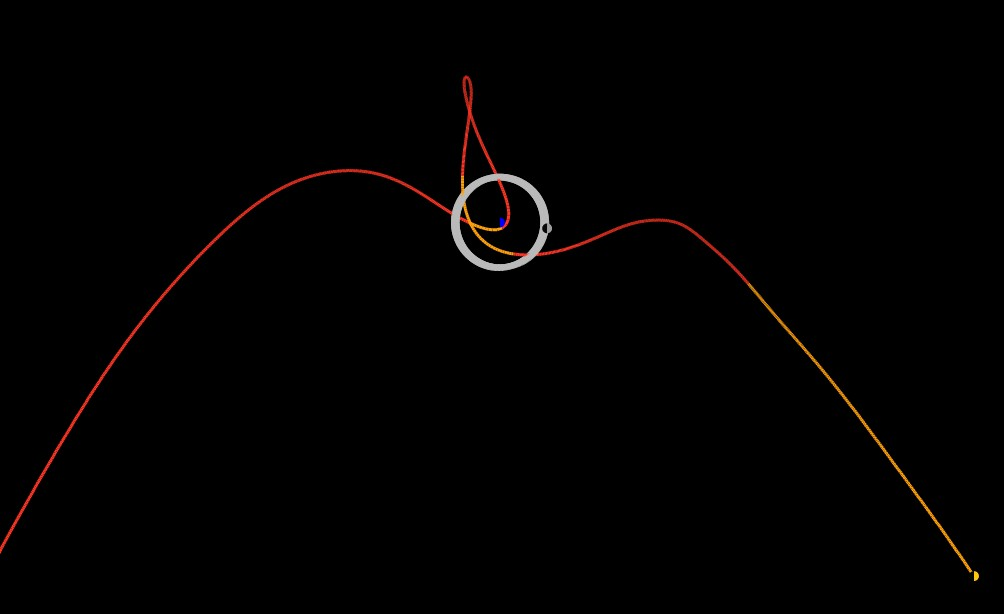
\includegraphics[width=\textwidth]{media/trajectories_2020SO.jpg}\\
		trajectories of objects in space \\
		\hyperref{https://en.wikipedia.org/wiki/2020_SO\#/media/File:2020SO_b.gif}{}{}{2020SO} 
	\end{minipage}
	\begin{minipage}[t]{0.25\textwidth}\centering
		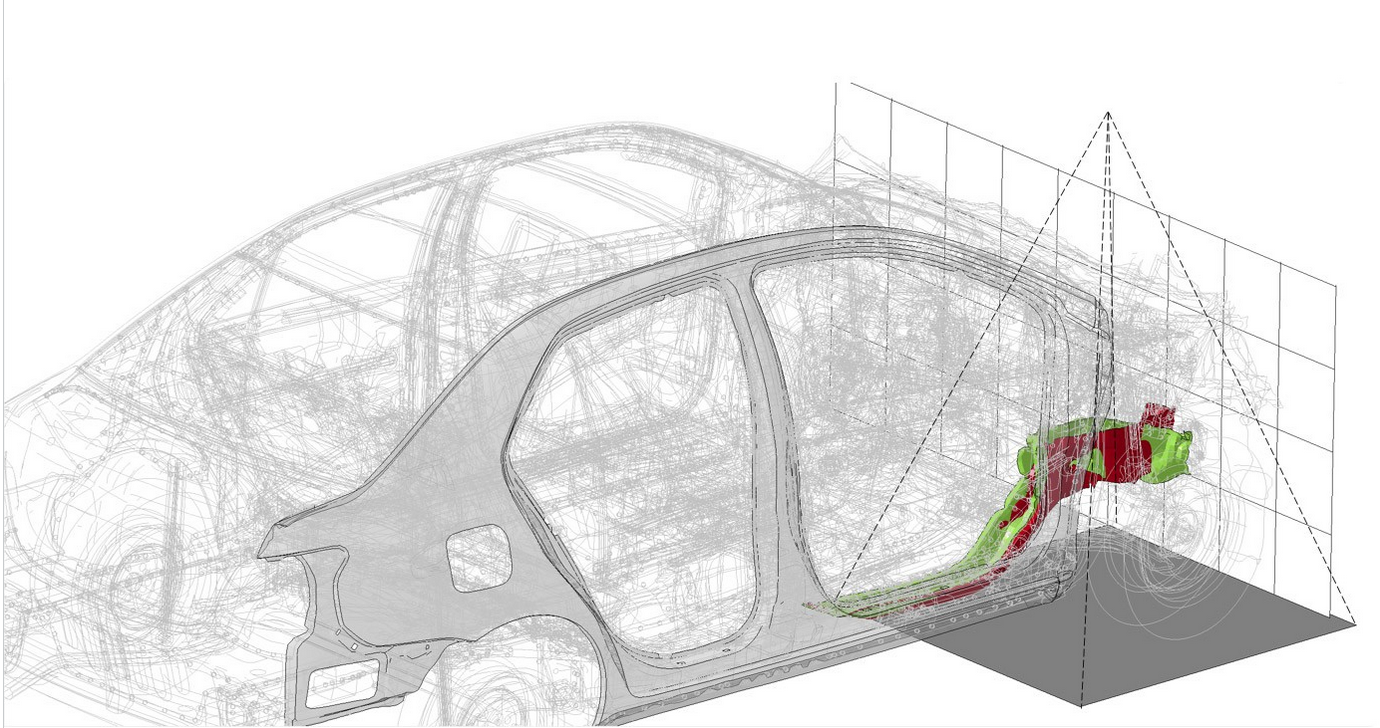
\includegraphics[width=\textwidth]{media/carcrash_sim.png}\\
		\hyperref{https://www.emi.fraunhofer.de/de/geschaeftsfelder/automotive/forschung/archiv/Roentgen-Crashtest.html}{}{}{car crash simulation} 
	\end{minipage}
	\begin{minipage}[t]{0.25\textwidth}\centering
		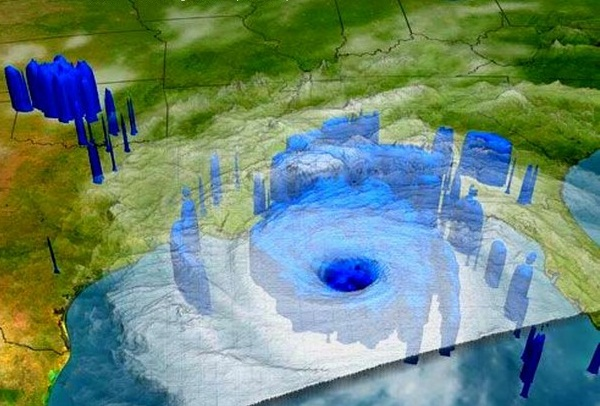
\includegraphics[width=\textwidth]{media/weather.jpg}\\
		\hyperref{https://en.wikipedia.org/wiki/Numerical_weather_prediction}{}{}{weather prediction} 
	\end{minipage}
	% CT SCAN
	\begin{minipage}[t]{0.25\textwidth} \centering
		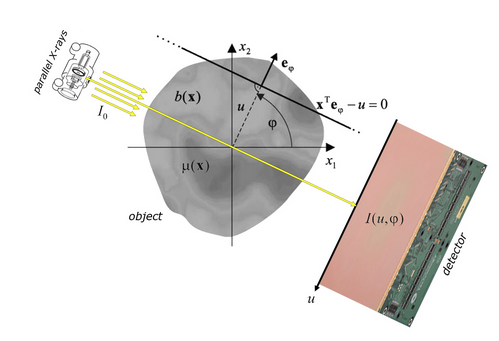
\includegraphics[width=\textwidth]{media/ct_scan.png}\\
		\hyperref{https://en.wikipedia.org/wiki/CT_scan}{}{}{CT Scan} 
	\end{minipage}
\end{frame}
%
\begin{frame}[c]
	\textbf{Relation to Data Science?}~\\
	\begin{itemize}
		\item due to the high amount of data available \textbf{data}-driven models are more important than ever \Vspace{0.2cm}
		\item data can be considered
		as a \textbf{mathematical object} (e.g., as a matrix/vector) \Vspace{0.2cm}
		\item with \textbf{numerical algorithms} we can manipulate data:\Vspace{0.2cm}
		\begin{itemize}\normalsize
			\item solve systems involving the data (fitting data, prediction,...)
			\vspace{0.2cm}\item extract the most important features (singular values, PCA, data compression,...) 
			\vspace{0.2cm}\item calibrate models against data (machine learning, neural networks,...)
		\end{itemize}
	\end{itemize}	
    \Vspace{2cm}
	\begin{minipage}[t]{0.25\textwidth}\centering
		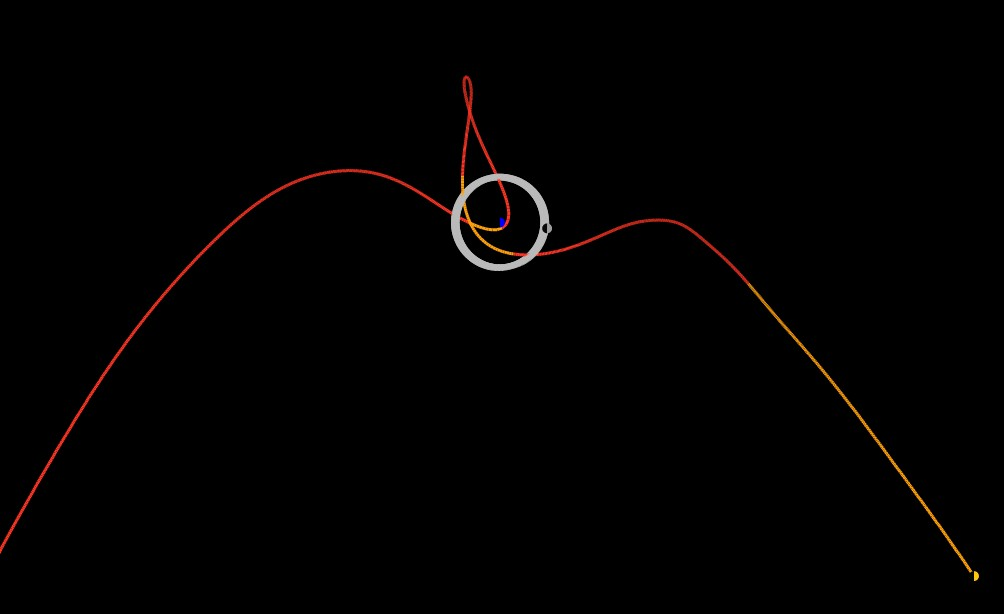
\includegraphics[width=\textwidth]{media/trajectories_2020SO.jpg}\\
		trajectories of objects in space \\
		\hyperref{https://en.wikipedia.org/wiki/2020_SO\#/media/File:2020SO_b.gif}{}{}{2020SO} 
	\end{minipage}
	\begin{minipage}[t]{0.25\textwidth}\centering
		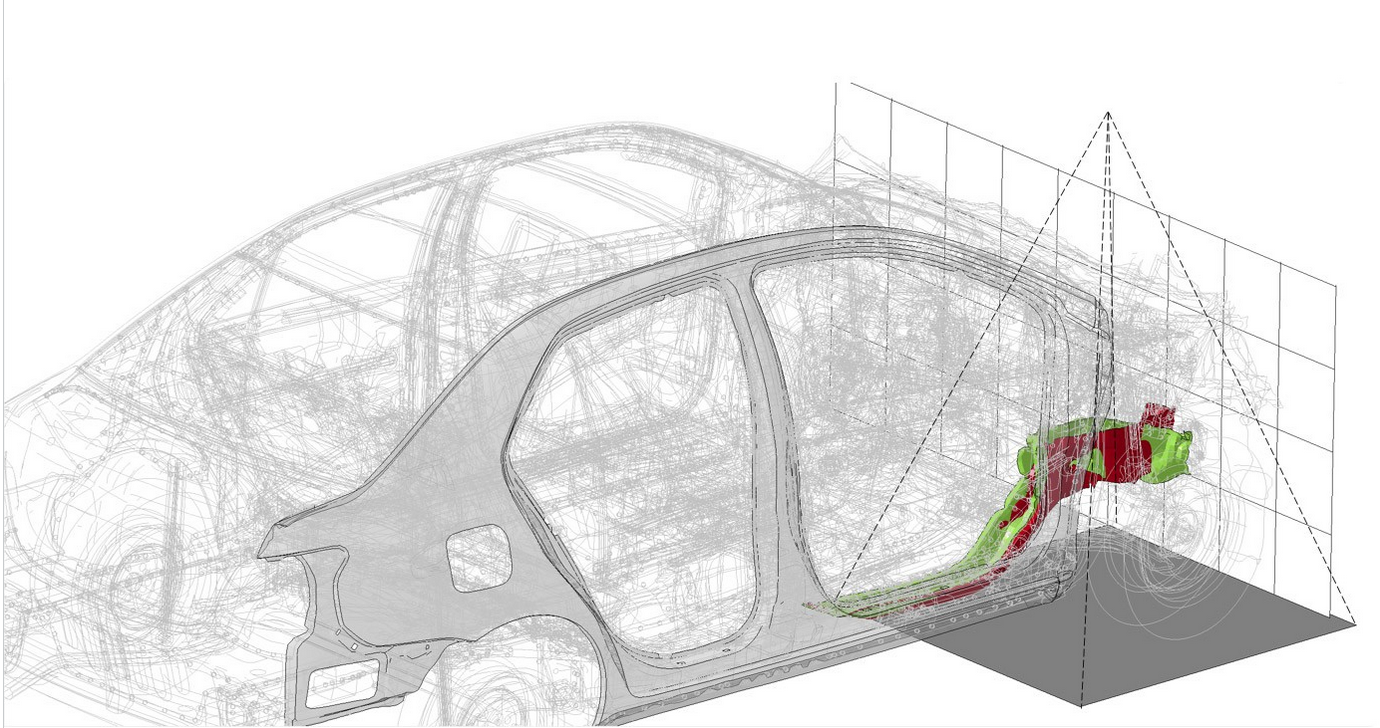
\includegraphics[width=\textwidth]{media/carcrash_sim.png}\\
		\hyperref{https://www.emi.fraunhofer.de/en/business-units/automotive/research/Roentgen-Crashtest.html}{}{}{car crash simulation} 
	\end{minipage}
	\begin{minipage}[t]{0.25\textwidth}\centering
		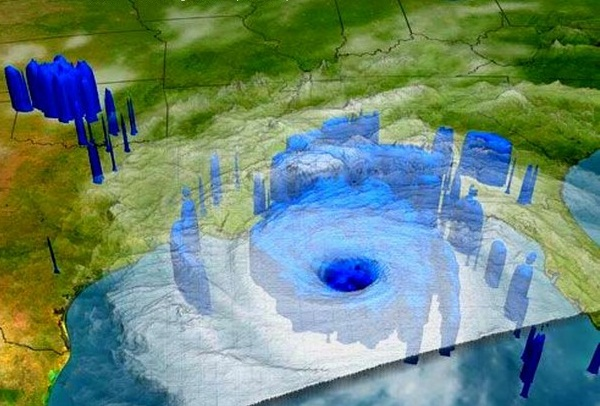
\includegraphics[width=\textwidth]{media/weather.jpg}\\
		\hyperref{https://en.wikipedia.org/wiki/Numerical_weather_prediction}{}{}{weather prediction} 
	\end{minipage}
	% CT SCAN
	\begin{minipage}[t]{0.25\textwidth} \centering
		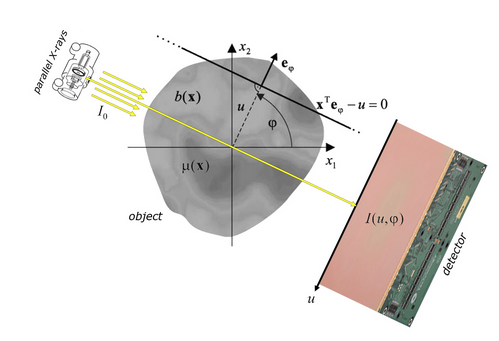
\includegraphics[width=\textwidth]{media/ct_scan.png}\\
		\hyperref{https://en.wikipedia.org/wiki/CT_scan}{}{}{CT Scan} 
	\end{minipage}
\end{frame}

%
\begin{frame}[c]
	\textbf{Preview}~\\
	\Vspace{0.25cm}
	Let us assume we have $m$ data points
	$$(z_i, y_i),~~~i=1,\ldots,m,$$
	where
	\begin{itemize}
		\item $z_i$ are $n$-dimensional vectors of \textit{explanatory features} 
		\item $y_i$ are $k$-dimensional vectors representing the \textit{response/prediction/classification}
	\end{itemize}
	~\\
	$\rightarrow$ \textit{The term \textit{``vector''} already indicates that Linear Algebra comes naturally into the game.}
	~\\~\\~\\
	\textbf{Examples}\\
	\begin{itemize}
		\item You ask $m$ persons about 
		\begin{align*}
		z_i &= (\text{age}, \text{sex},\text{weight},\text{height},\text{years of experience}) &(n=5 ~ \text{dimensional vector})\\
		y_i &= \text{salary} &(k=1 ~ \text{dimensional vector})
		\end{align*}
		\item Consider $m$ years where
		\begin{align*}
		z_i &= \text{year} &(n=1 ~ \text{dimensional vector})\\
		y_i &= \text{global mean temperature} &(k=1 ~ \text{dimensional vector})
		\end{align*}	
		\item Consider $m$ images that you want to classify 
		\begin{align*}
		z_i &=(p_{lj})_{lj} & (\text{image stored as matrix/vector})\\
		y_i &= (\text{dog}, \text{cat}, \text{elephant}) &(k=3 ~ \text{dimensional vector})
		\end{align*}
	\end{itemize}
	
\end{frame}

\begin{frame}[c]
	\textbf{\large  Dealing solely with the features $z$}~~\\~\\
	Applications of the \textbf{Singular Value Decomposition} are:\\
	% Consider just the $m$ $n$-dimensional feature vectors $z_i$:\\~\\
	~\\~\\
	\begin{minipage}[t]{0.48\textwidth}
		\textbf{Principal Component Analysis (PCA)}\\~\\
		{\raggedright
			$\rightarrow$ Aim: dimension reduction\\~\\}
		{\centering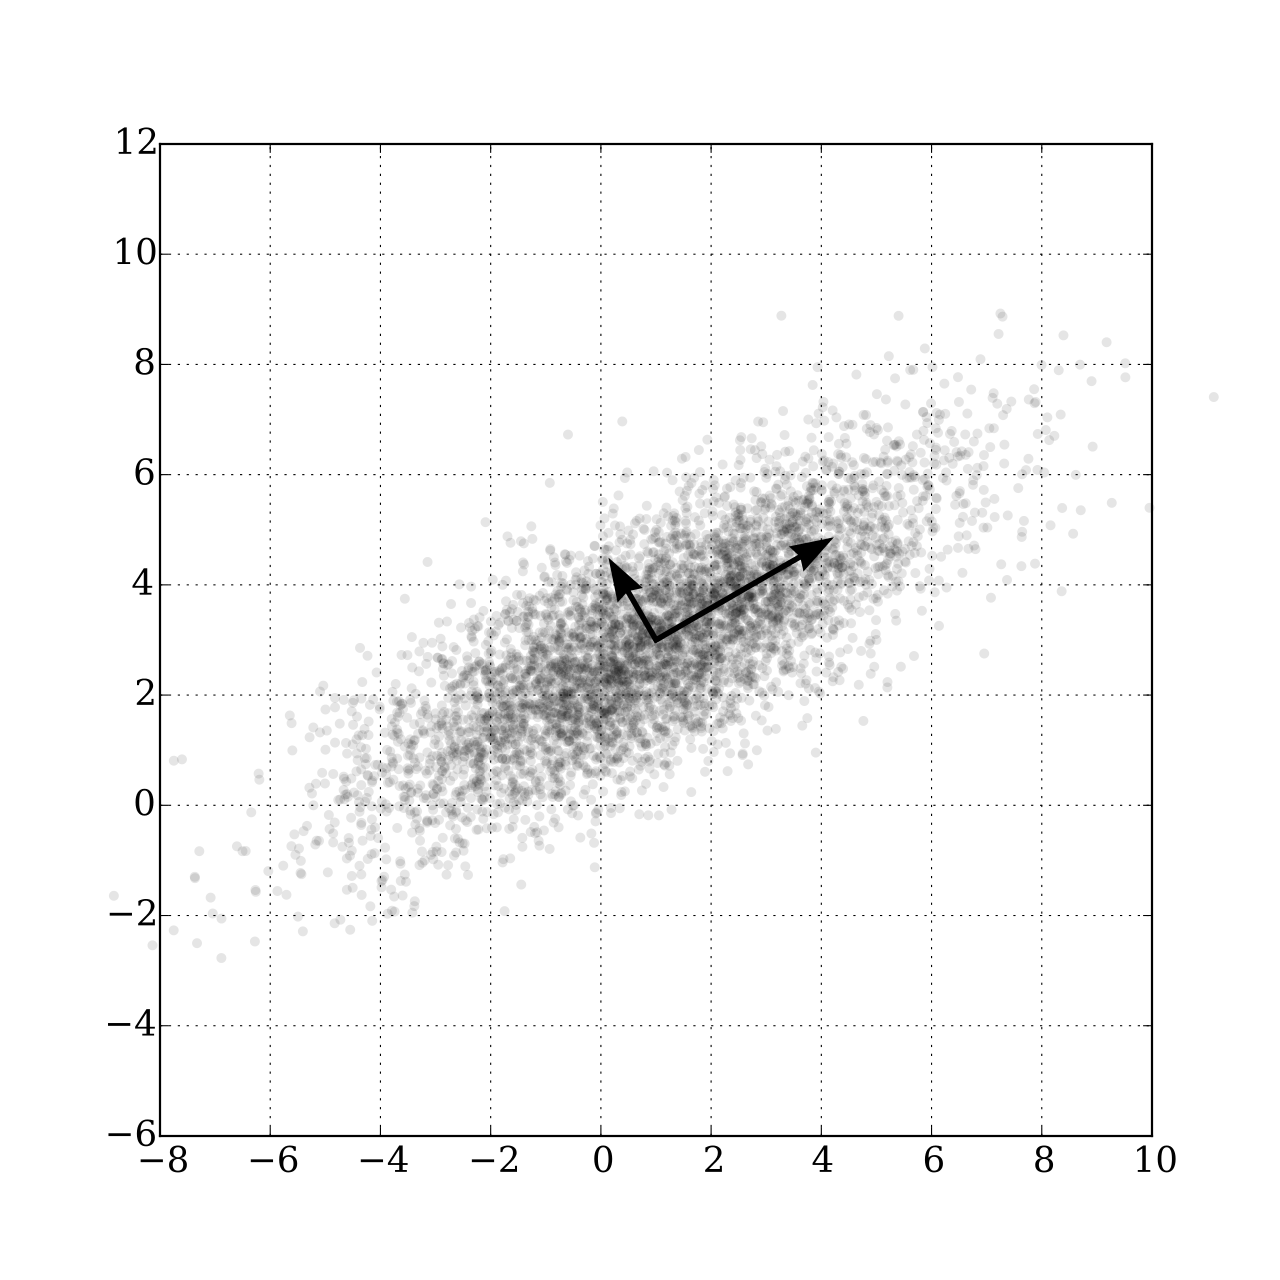
\includegraphics[width=0.77\textwidth]{media/PCA.png}}
	\end{minipage}
	~~~~~
	\begin{minipage}[t]{0.48\textwidth}
		\textbf{Data compression}\\~\\
		\raggedright
		$\rightarrow$ Aim: compression without dimension reduction\\~\\
		{ \hspace*{-0.6cm}\centering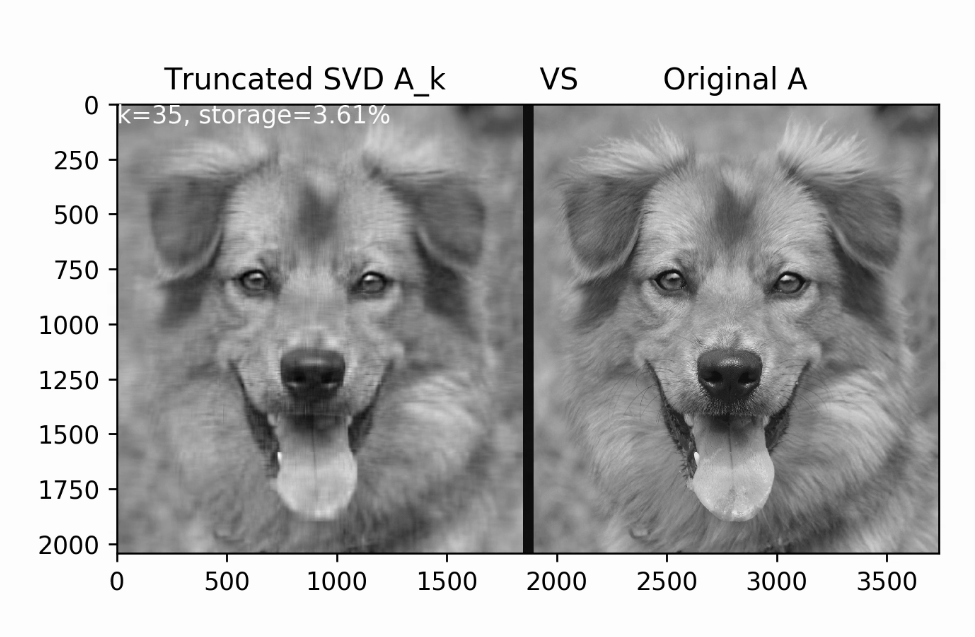
\includegraphics[width=1.1\textwidth]{media/SVD_dog.png}}
	\end{minipage}
\end{frame}
%
\begin{frame}[c]
	\textbf{\large  Relating features $z$ to response $y$}~\\~\\
	One central goal in many scientific fields is to find a \textbf{model} $f_x$ depending on some parameters $x=(x_i)_i$, which ``best'' explains the relation between $z_i$ and $y_i$ in the sense that 
	$$f_x(z_i) \approx y_i,~~~\text{for all}~~i=1,\ldots,m$$
	\begin{itemize}
		\item  \textbf{The task:} Find those parameters $x$ for which the ``distance'' between our prediction  $f_x(z_i)$ and the measured response $y_i$ is ``as small as possible''.\\
		\item Math gives us the tools to rigorously define this task, to analyze it systematically and to provide numerical solutions!
		~\\
	\end{itemize}
~\\
	\textbf{Curve Fitting}
		$$f_x(z) := x_0 + x_1z + x_2 z^2$$
		\\ \centering
		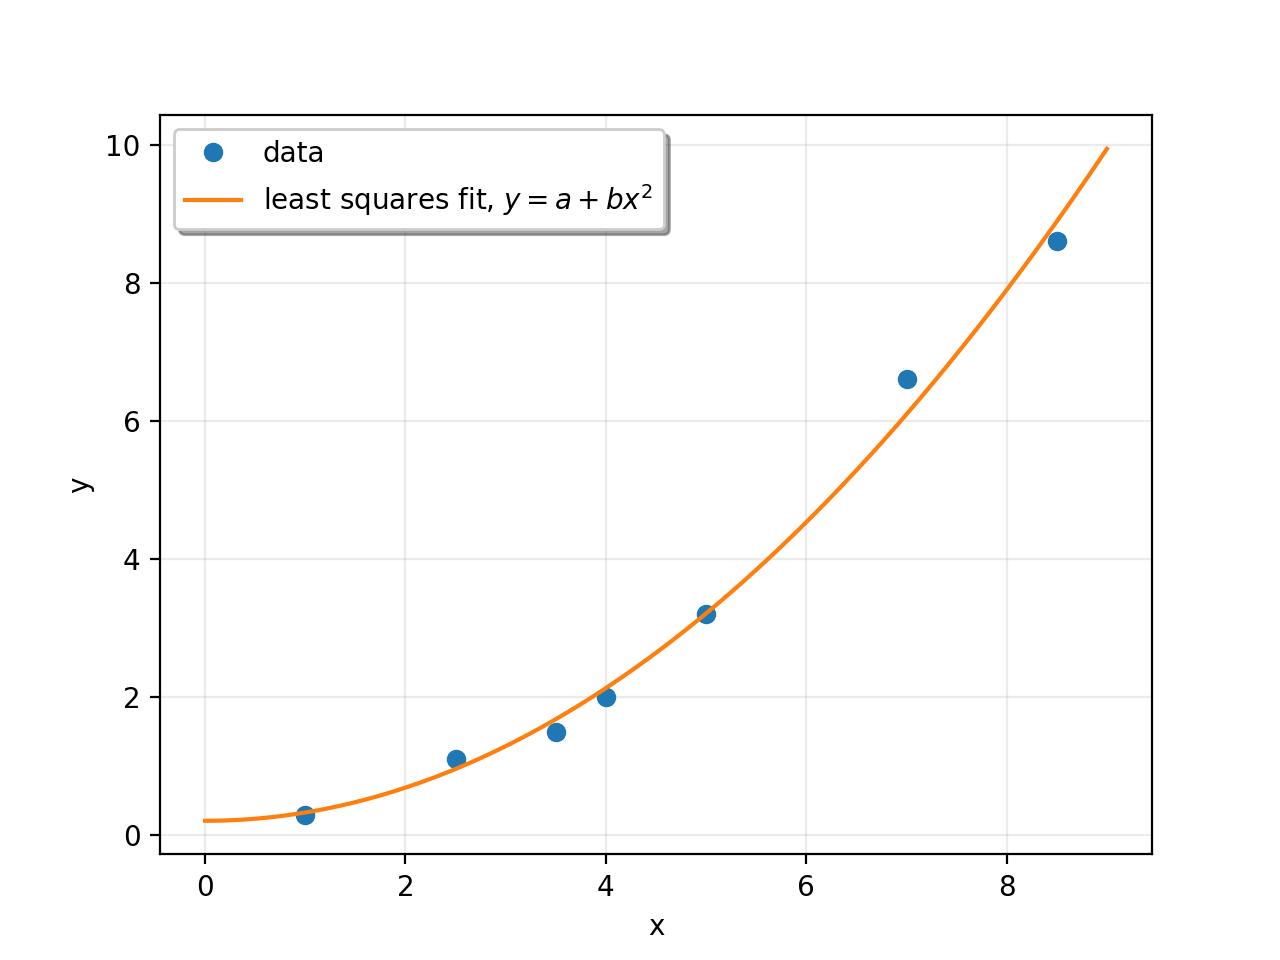
\includegraphics[width=0.37\textwidth]{media/4_least_squares.png}\\
\end{frame}

\begin{frame}[c]
	\textbf{Simple image inpainting}
	\vspace*{-0.3cm}
	$$\min_x \|Ax-b\|^2 + R(x)$$
	\begin{center}
		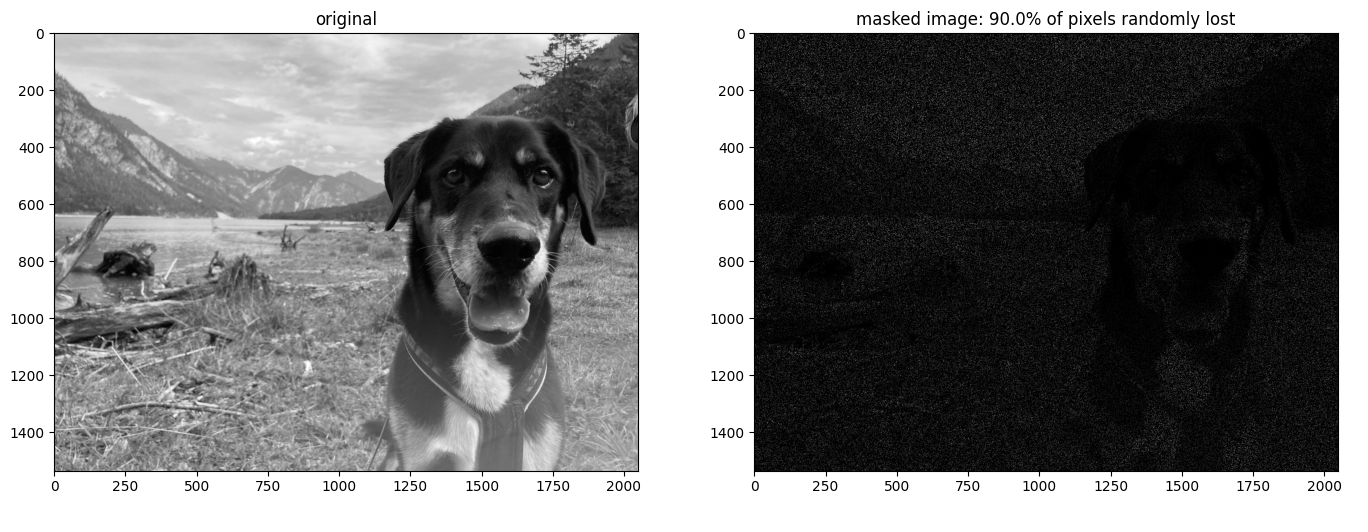
\includegraphics[width=0.8\textwidth]{media/Image_Inpainting-1.png}\\
		\vspace*{-0.3cm}
		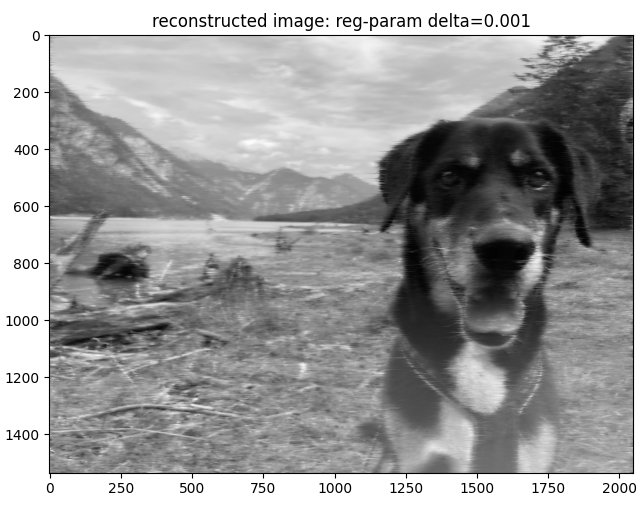
\includegraphics[width=0.45\textwidth]{media/Image_Inpainting-2.png}	
	\end{center}
\end{frame}

\begin{frame}[c]
\begin{center}
		 \begin{minipage}{0.8\textwidth}
		 \textbf{\Large Take away message}\\~\\
	 	Math provides a rigorous framework of abstract structures (Definition) within which their properties and relations (Theorem) can be systematically analyzed (Proof).
	 	~\\~\\
	 	The same mathematical concept can be exploited in multiple applications; see, e.g., SVD above.
	 	~\\~\\
	 	Given a real-world problem the user has to provide an interface (a mathematical model) to these  concepts to make use of the mathematical theory.
	 \end{minipage}
\end{center}
\end{frame}

%%%%%%%%%%
% CONTENT
%%%%%%%%%%
\AtBeginLecture{
	\only<presentation>{\frame[noframenumbering,c]{
		~\\~\\	
		\begin{center}
			\begin{minipage}{0.8\textwidth}
				\bf \Large \insertlecture~\\~\\
			\end{minipage}
		\end{center}					
}
}
}


% basics
\only<presentation>{\setnextsection{0}}
\lecture{Math Basics}{basics}
% !TeX spellcheck = en_US

% STATEMENTS
\begin{frame}
	\Section{Mathematical Basics}
	In this first section we will provide mathematical notations and concepts which are fundamental and crucial for the further presentation.\\
	\vspace{0.2cm}
	\Subsection{Statements}
		\vspace{0.2cm}
	By a \textbf{statement} we mean a linguistic or mental construction that is either true or false.
	\vspace{0.2cm}
	\begin{ex}~\\\vspace{0.1cm}
		\begin{itemize}
		\item ``4 is an even number.'' is a true statement.
		\item ``Bananas have conic shape.'' is a false statement.
		\item ``In the night, it is colder than outside.'' is not a statement.
		\item ``There are infinitely many stars.'' is a statement, because it can be true or false.
		\end{itemize}
	\end{ex}
	\vspace{0.2cm}
	\textbf{Relations and Operations}
	\color{defgruen}
	\begin{center} \vspace{-0.1cm}
		\begin{tabular}[t]{ll}
			$\neg A$: & $A$ is false (\textbf{negation})\\\vspace{0.2cm}
			$A\Rightarrow B$: & from $A$ follows $B$; if $A$ is true, then also $B$ is true (\textbf{implication})\\\vspace{0.2cm}
			& we say: $A$ is \textbf{sufficient} for $B$, $B$ is \textbf{necessary} for $A$\\\vspace{0.2cm}
			$A\Leftrightarrow B$: & $A$ is true, if and only if  $B$ is true. (\textbf{equivalence})
		\end{tabular}
	\end{center}
\color{fontcolor}
	Note that the following two statements are equivalent
	\begin{align*}
	\color{satzrot}A&\color{satzrot}\Rightarrow B\\
	\color{satzrot}\neg B&\color{satzrot} \Rightarrow \neg A 
	\end{align*}
\Hide{
For example $A$: ``it rains'', $B$: ``the street is wet'', then $\neg A$: ... and $\neg B:$ ...	
}
\end{frame}

\mode<article>{
\begin{center} \vspace{-0.1cm}
	\begin{tabular}[t]{ll}
		$A\wedge B$: & $A$ and $B$ are true (\textbf{and})\\
					$A\vee B$: & $A$ or $B$ is true (\textbf{or})\\
					$A\:\dot\vee\: B$: & either $A$ or $B$ is true (\textbf{excl. or})\\

	\end{tabular}
\end{center}
}

\begin{frame}
\Subsection{Sets}
 \begin{defi}[Set]\label{def:set}
 	According to \textsc{Cantor}\index{Cantor@\textsc{Cantor}} a \textbf{set} is a well-defined collection of distinct objects, considered as an object in its own right. The objects that make up a set (also known as the set's \textbf{elements}) can be anything: numbers, people, letters of the alphabet, other sets, and so on. 	 
 \end{defi}
\vspace{0.1cm}
 \textbf{Notation:} curly brackets $\{ \}$
 \vspace{0.1cm}
 \begin{ex} \label{ex:sets}~\\
 	\blank
 	\begin{itemize}
 		\blank
 		\item[\blank$\bullet$] $M := \{ 1,2,3 \}$
 		\item[\blank$\bullet$] $N := \{ \underbrace{x}_{\text{\scriptsize element}} \,|\, \underbrace{\text{$x$ is multiple of } ~7}_{\text{\scriptsize element property}} \}= \{ x \,\colon\, \text{$x$ is multiple of }~ 7 \} = \{7,14,21,\ldots\}$ \vspace{0.2cm}
 	\end{itemize}
  $\rightarrow$ Note: We use ``$:=$'' for definitions\\
 \end{ex}
\vspace{0.6cm}
\begin{defi}[Cardinality]\label{def:cardinality}
If a set $M$ is \textbf{finite} (i.e., it only contains finitely many elements), then we denote by $|M|$ the number of elements contained in $M$ and call it \textbf{cardinality of $M$}.
\end{defi}
\end{frame}

\begin{frame}
\textbf{\large Set relations and further definitions}\\
\vspace{0.2cm}
\begin{table}[h] \color{defgruen}
	\begin{tabular}[t]{ll}
		$a \in M$ (or $M \ni a$): & $a$ is element of $M$; $M$ contains $a$\\\vspace{0.2cm}
		$a \not\in M$ (or $M \not\ni a$): & $a$ is not element of $M$; $M$ does not contain $a$
	\end{tabular}
\end{table}	 
{\blank
$M = \{1,2,3\}$, $1 \in M$, $\{1\} \notin M$
	\vspace*{0.4cm}
}
\begin{table}[h] \color{defgruen}
	\begin{tabular}[t]{ll}
		$M=N$: & $M$ contains the same elements as $N$\\\vspace{0.2cm}
		$M\not=N$: & $M$ does not contain the same elements as $N$
	\end{tabular}
\end{table}

{\blank
	$N := \{1,2\}$,  $M=M$, $M \neq N$
	\vspace*{0.4cm}
}

\begin{table}[h] \color{defgruen}
	\begin{tabular}[t]{ll}
		$M \subset N$ (or $M\subseteq N$): & $M$ is subset of $N$, i.e., each element of $M$ is also \\\vspace{0.2cm}
		& an element of $N$; equality of sets is permitted.\\\vspace{0.2cm}
		$N \supset M$ (or $N\supseteq M$): & $N$ is superset of $M$; analogously\\\vspace{0.2cm}
		$M \subsetneqq N$: & $M$ is strict subset of $N$; $M\not=N$\\\vspace{0.2cm}
		$\emptyset = \{\}$: & empty set
	\end{tabular}
\end{table}
{\blank
	$N \subset M$ and even $N \subsetneqq M$; what about the relation between $N_2 :=\{\{1\}, 2\}\}$ and  $M$ or $\emptyset$ and  $M$?
\vspace*{0.4cm}
}
~\\
\textbf{Remark:} Very useful in practice to show that two sets are equal: \\
$$M=N \iff M\subset N \textbf{~~and~~} N \subset M $$
\end{frame}

\begin{frame}
	\begin{table}[h] \color{defgruen}
		\begin{tabular}[t]{ll}
			$M \times N$: & \textbf{Cartesian product} defined by 
			$M \times N :=\{(m,n)\colon m\in M,n\in N  \}$\vspace{0.2cm}\\\vspace{0.4cm}
			& $M^n := M \times \ldots \times M$ ($n$ times)
		\end{tabular}
	\end{table}
{
	\blank
Let us consider $$M:=\{ x : \text{$x$ is multiple of } ~2 \} = \{2, 4, 6, \ldots\}$$ and 
$$N:=\{ x : \text{$x$ is multiple of } ~4 \} = \{4, 8, 12, \ldots\},$$ then we have\\ 
$$M \times N = \{(a,b): a\in M, ~b\in N\} = \{ (2,4), (2,8),\ldots, (4,4), (4,8), \ldots \}$$ \\~\\
\textit{\small \color{header}[image:Cartesian grid]}
}
\end{frame}

\begin{frame}
\begin{table}[h] \color{defgruen}
	\begin{tabular}[t]{ll}
	$\mathcal{P} (M)$  & \textbf{power set of $M$} defined by\\
	&$\mathcal{P} (M) := 2^M :=\{ N: N\subset M\} $ (set of all subsets of $M$)\\
	&\vspace{0.2cm}We find $|\mathcal{P} (M)| = 2^{|M|}$
\end{tabular}
\end{table}
{
	\blank~\\

 Let us consider $M=\{ 1,2\}$, then $|M|=2$ and the power set of $M$ is given by
	\[\mathcal{P}(M)=2^M=\bigl\{\emptyset ,\{ 1\},\{ 2\},\{ 1,2\}\bigr\}.\]
	We also find
	$$|\mathcal{P}(M)|=4 = 2^{|M|}=2^2 . $$
	~\\
	Remark: \textbf{Binomial theorem}
	$$ \sum_{k=0}^n 	\binom{n}{k} =2^n,  $$
	where $$\binom{n}{k} := \frac{n!}{k!(n-k)!}$$ is the so-called binomial coefficient, which give us the number of subsets with $k$ elements that we can draw from a set with $n$ elements.

}
\end{frame}



\begin{frame}
	\textbf{\large Summary: Set relations and further definitions}\\
	\vspace{0.2cm}
	\begin{table}[h] \color{defgruen}
		\begin{tabular}[t]{ll}
			$a \in M$ (or $M \ni a$): & $a$ is element of $M$; $M$ contains $a$\\\vspace{0.2cm}
			$a \not\in M$ (or $M \not\ni a$): & $a$ is not element of $M$; $M$ does not contain $a$\\[3pt]
			$M=N$: & $M$ contains the same elements as $N$\\\vspace{0.2cm}
			$M\not=N$: & $M$ does not contain the same elements as $N$\\\vspace{0.2cm}
			$M \subset N$ (or $M\subseteq N$): & $M$ is subset of $N$, i.e., each element of $M$ is also \\\vspace{0.2cm}
			& an element of $N$; equality of sets is permitted.\\\vspace{0.2cm}
			$N \supset M$ (or $N\supseteq M$): & $N$ is superset of $M$; analogously\\\vspace{0.2cm}
			$M \subsetneqq N$: & $M$ is strict subset of $N$; $M\not=N$\\\vspace{0.2cm}
			$\emptyset = \{\}$: & empty set\\\vspace{0.2cm}
			$M \times N$: & \textbf{Cartesian product} defined by 
			$M \times N :=\{(m,n)\colon m\in M,n\in N  \}$\\\vspace{0.4cm}
			& $M^n := M \times \ldots \times M$ ($n$ times)\\\vspace{0.2cm}
			$\mathcal{P} (M)$  & \textbf{power set of $M$} defined by\\
			&$\mathcal{P} (M) := 2^M :=\{ N: N\subset M\} $ (set of all subsets of $M$)\\
			&\vspace{0.2cm}We find $|\mathcal{P} (M)| = 2^{|M|}$
		\end{tabular}
	\end{table}
\end{frame}






\begin{frame} 
\textbf{\large Set operations} ~\\ 
\vspace{0.2cm}
$$\begin{array}{llll} 
M \cup N &:=& \lbrace a: a\in M \text{ or } a \in N\rbrace&\text{(\textbf{\color{defgruen}union})}\\[3pt]
M \cap N &:=& \lbrace a: a\in M \text{ and } a \in N\rbrace&\text{(\textbf{\color{defgruen}intersection})}\\[3pt]
M \setminus N &:=& \lbrace a : a\in M \text{ and } a \not\in N\rbrace&\text{(\textbf{\color{defgruen}difference})}\\[6pt]
\text{If}~N\subset M&&&\\[6pt]
 N^c  &:=&  \overline{N}:= M \setminus N&\text{(\textbf{\color{defgruen}complement of N with respect to M})}\\[3pt]
%  M \dot\cup N &=& M \cup N  \text{~~if~~} M\cap N = \emptyset  &  \text{(disjoint union)}
\end{array}$$ 
~\\\vspace{0.3cm}
$M, N$ are called \textbf{\color{defgruen}disjoint}\index{disjoint},  if $M \cap N = \emptyset$.
%
\vspace{0.5cm}
\begin{ex} \label{ex:set_operations}
	~\\
	\blank
	Let $M = \{1,2,3, 4\}$ and $N = \{1,3\}$, then\vspace{0.2cm}
	\begin{itemize}
		\blank
		\item[] $M \cup N = \{1,2,3, 4\}$, we always have $M \subset M\cup N$ and  $N \subset M\cup N$ \vspace{0.2cm}
		\item[] $M \cap N = \{1, 3\}$\vspace{0.2cm}
		\item[] $\overline{N} =M \setminus N = \{2, 4\}$
	\end{itemize}
\end{ex}
\vspace{0.2cm}

\end{frame}

% DE MORGAN
\begin{frame}
For combinations of those set operations we have the following result: \vspace{-0.2cm}
 \begin{lemma}[\textbf{\textit{De Morgan's laws}}]\label{lem:demorgan}
 	Let $\Omega$ be a set and $M,N \subset \Omega$. Then we find
 	\begin{itemize}
 		\item[i)] $ (M\cup N)^c  = M^c \cap N^c $,
 		\item[ii)] $ (M\cap N )^c =  M^c \cup  N^c $.
 	\end{itemize}
 Here the complements are taken with respect to $\Omega$.
 \end{lemma}\vspace{-0.5cm}
 \begin{proof}
 	\textit{Exercise.}
 \end{proof}
{
	\blank
	~\\
	Illustration:\\
	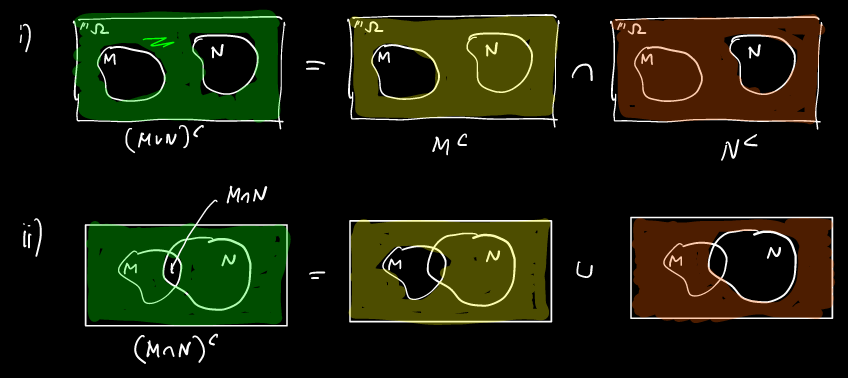
\includegraphics[width=0.8\textwidth]{./media/venn-diagram.png}
}
\end{frame}
 
\begin{frame}
%functionS
\Subsection{Functions}
\begin{defi}[\textbf{\textit{function}}]\label{def:function}
	Let $M, N$ be two sets. A \textbf{function} or \textbf{mapping} $f$ from $M$ to $N$ (notation: $f\colon M\to N$) is determined by
	\begin{itemize}
		\item[] its \textbf{domain} $M$, 
		\item[] its \textbf{codomain} $N$,
		\item[] and a \textbf{rule},
	\end{itemize} 
that uniquely assigns to each element $a\in M$ an $b:=f(a)\in N$ (notation: $a \mapsto f(a)$).	 
\end{defi}
Two functions $f_1: M_1\to N_1$ and $f_2: M_2\to N_2$ are called \textbf{equal} (abbr.~$f_1\equiv f_2$) (identical),
if $M_1=M_2$, $N_1=N_2$ and $f_1(a)=f_2(a)$ for all $a\in M_1$ (i.e., equal, domain, codomain and rule).
%
	
\vspace{0.4cm}
\begin{ex}\label{ex:image_preimage_graph}
	~\\
	\blank
	Let $M := N :=\{1,2,3,4,5\ldots\}$ and consider $f\colon M \to N,~ a \mapsto 2a$. How could we ``visualize'' this function?\\ \vspace{0.2cm}
	i) a \textbf{table} with two columns (one for domain and codomain each)
	\begin{itemize}
		\blank
		\item[] follow where points go from $A=\{1,2\}\subset M$ 
		\item[] find points which would produce $B=\{4,6\} \subset N$
	\end{itemize}\vspace{0.2cm}
	ii) draw the \textbf{graph} into a coordinate system
\end{ex}
\end{frame}

\begin{frame}
	We introduce function related sets: \vspace{-0.3cm}
	\begin{defi}[{\textit{Image, preimage, graph}}]\label{def:image_preimage_graph}
		Let $A \subset M$ and $B \subset N$, then
		\begin{itemize} \color{defgruen}
			\item[i)] the set $f(A) = \{f(a) : a\in A\} \subset N$ is called \textbf{image set} of $A$ (under $f$),
			\item[ii)] the set $f^{-1}(B)=\lbrace a\in M: f(a)\in B\rbrace \subset M$ is called \textbf{preimage} of $B$ (under $f$),
			\item[iii)] the set $\text{graph}(f) := \{(a,f(a))\colon a \in M\} \subset M\times N$ is called the \textbf{graph} of $f$.
		\end{itemize} 
	\end{defi}
	$\rightarrow$ \textbf{Attention:} Here, $f^{-1}$ is not the inverse function (see below).\\ \vspace{0.2cm}
	~\\
	{\blank
	-- {\small\color{header}[abstract picture with  with image, preimage and graph]}\\
	-- With the definitions from above we have
	\begin{itemize}
		\blank
		\item[] for $A=\{1,2\}$ we find $f(A) = \{2,4\}$
		\item[] for $B=\{4,6\}\}$ we find $f^{-1}(B) = \{2,3\}$
		\item[] $\text{graph}(f) = \{(1,2), (2,4), (3,6), \ldots\}$
	\end{itemize}
}	
\end{frame}


 
\begin{frame}
Important properties of functions: \vspace{-0.3cm}
\begin{defi}[\textbf{\textit{Injective, surjective, bijective}}] \label{def:injective_surjective_bijective}
	A function 	$f: M\to N$ is called
	\begin{itemize}
	\item[i)] \textbf{injective} (one-to-one), if $f(a)\not=f(\tilde a)$ for all $a,\tilde a\in M$ with $a\not=\tilde a$;
	\item[ii)] \textbf{surjective} (onto), if for all $b\in N$ there exists an $a\in M$ with $f(a)=b$ (or equivalently $f(M)=N$);
	\item[iii)] \textbf{bijective}, if $f$ is injective as well as surjective  relation.
	\end{itemize}
\end{defi}
%
\vspace{0.3cm}
We can invert bijective functions:\vspace{-0.3cm}
\begin{defi}[\textbf{\textit{Inverse function}}] \label{def:composition}
	Let $f\colon M\to N$ be a bijective (invertible) function. Then there exists a (unique) function $f^{-1}\colon N \to M$, the so-called \textbf{inverse of $f$}, such that
	$$f(a) = b \iff f^{-1}(b) = a.$$ 
\end{defi}
%
\vspace{0.3cm}
\begin{ex}
	\blank
 Consider again example from above and the visualization with the help of the table.
\end{ex}
\end{frame}

\begin{frame}
\vspace{0.3cm}
We can concatenated two or more functions:\vspace{-0.3cm}
\begin{defi}[\textbf{\textit{Composition}}] \label{def:composition}
	Let $f\colon M\to N$ and $g\colon N\to P$ be functions, then we call the function
	$$g\circ f\colon M\to P,~ a \mapsto g(f(a))$$
	\textbf{composition} of $f$ and $g$. 
\end{defi}
%
{	\blank
	~\\
-- {\small\color{header}[abstract picture for composition of the functions}\\
	-- Concrete example:
	\begin{align*}
	&M=\{1,2,3,4,\dots\},~N:=\{x:~x~\text{is even}\},~P:=\{x:~x~\text{is odd}\},\\
	&f:M\rightarrow N, a\mapsto 2a,~g:N\rightarrow P, b\mapsto b-1
	\end{align*}
	$$
	(g\circ f)(6)=g(\underbrace{f(6)}_{=12})=g(12)=12-1=11
	$$
}
\noindent A function with ``no effect'':\vspace{-0.3cm}
\begin{defi}[\textbf{\textit{Identity function}}] \label{def:identity}
	Let $M$ be a set. Then the function 
	$$id := id_M \colon M \to M, ~a\mapsto a $$
	is called the \textbf{identity function on $M$}.
\end{defi}

 \end{frame}





% QUANTORS and AIM of MATH
\only<article>{
\begin{frame}
If $M$ is a set and $P$ a property, which an element $a\in M$ can have. Then, we use the abbreviations for certain statements: 
\ite
\item {\color{defgruen}$\forall {a\in M}\,:\, a$ has property $P$}\\
means: each $a\in M$ has property $P$ \qquad
(``$\forall$'' is called \textbf{all quantor})
\item {\color{defgruen}$\exists {a\in M}\,:\, a$ has property $P$}\\
means: there is at least one $a\in M$ with property $P$\qquad
(``$\exists$'' is called \textbf{existence quantor})
\item {\color{defgruen}$\exists_1{a\in M}\,:\, a$ has property $P$}\\
means: there is  \textbf{exactly one} $a\in M$ with property $P$
\eti
%
\vspace{0.3cm}
Note the interesting equivalences
\begin{align*}
\color{satzrot}\neg(\forall {a\in M}\,:\, a \text{ has property }P)& \color{satzrot}\Longleftrightarrow \exists {a\in M}\,:\, a \text{ does not have property }P\\
\color{satzrot}\neg(\exists {a\in M}\,:\, a \text{ has property }P)& \color{satzrot}\Longleftrightarrow \forall {a\in M}\,:\, a \text{ does not have property }P
\end{align*}
\begin{ex}\label{ex:quantors}
	\blank
	content...
\end{ex}
%
\textit{Aim of mathematics: make nontrivial statements about certain structural objects.
	However, its whole theoretical construction cannot be founded on nothing. As a foundation, we formulate a minimum number of plausible axioms, which are not and cannot be proved.}
\textit{In particular, we need axioms for the definition of \textbf{numbers.} The \textsc{Peano} axioms give the natural numbers $\N$, from which negative and rational numbers can be constructed. A further axiom gives the real numbers $\R$. }
 \end{frame}
}



 

 
\begin{frame}
\Subsection{Numbers} \label{numbers}
%\only<presentation>{	\tableofcontents[currentsubsection]}
The notion of \textbf{number} has been extended over the centuries, here we do not go in detail through the axiomatic construction but just point out some properties that are useful in the remaining.\\
\vspace{0.5cm}
Here is an overview:\\
\begin{table}
	\centering
	\begin{tabular}{c|c|c|l}
		$\N$ & \textbf{Natural} 	& $\{1,2,3,4, 5, \ldots\}$ & counting objects\\
		&&&\textbf{order relation}: $m\le n$\\
		&&&$m+n$, $m\cdot n$\\
		&&&proof concept of \textbf{induction} \\[0.3cm]
		%
		$\Z$ & \textbf{Integer} 	& $\{ \ldots,-3,-2,-1,0,1,2,3, \ldots\}$ & adding zero and negative numbers (borrowing money,...)\\ 
		&&&$(\Z, +)$ \textbf{ordered, commutative group}\\[0.3cm]
		%
		$\Q$ & \textbf{Rational} & $\left\lbrace \frac{p}{q}: ~p,q\in \Z, q \neq 0 \right\rbrace $& adding fractions of objects (one half of a cake)\\
		&&&$(\Q, +, \cdot)$ \textbf{ordered field}\\[0.3cm]
		%
		$\R$ & \textbf{Real} 	& $ \Q \cup \{\text{limits of sequences in } \Q\}$ & adding square roots ($\sqrt{2}$,$\sqrt{5}$,...), $\pi$,...\\
		&&&$(\R, +, \cdot)$ \textbf{ordered and complete field} \\[0.3cm]
		%
		$\C$ & \textbf{Complex}  & $\{a+ib:~a,b\in \R\}$, $i:= \sqrt{-1}$  & adding e.g. square root of negative numbers\\
		&&&$\R \times \R$~ \text{with a special multiplication}\\
		&&&$(\C,+, \cdot)$ \textbf{complete field} (not ordered)
	\end{tabular}
	\label{tab:numbers}
\end{table}
We have
$$\N ~~\subsetneqq~~ \Z~~  \subsetneqq~~   \Q ~~ \subsetneqq ~~  \R~~  \subsetneqq~~  \C $$ 
\end{frame}

\only<article>{
% NATURAL NUMBERS and % INTEGERS
\begin{frame}
\Subsubsection{Natural Numbers $\N$}
\vspace{0.5cm}
$\color{defgruen}\N:=\{1,2,3,\ldots\}$
\vspace{0.5cm}
\begin{itemize}
	\item most intuitive concept; counting objects \vspace{0.2cm}
	\item in mathematics rigorously defined through \textbf{the Dedekind-Peano Axioms} \vspace{0.2cm}
	\item (binary) operations on natural numbers: \vspace{0.2cm}
	\begin{itemize}  \normalsize
		\item summation: $m+n$ (commutative) \vspace{0.2cm}
		\item multiplication $m \cdot n$ (commutative) \vspace{0.2cm}
	\end{itemize}
	\item The natural numbers have an \textbf{order relation}: $m\le n$	 \vspace{0.2cm}
	\item Each natural number has a successor and thereby gives the proof concept of \textbf{induction}
\end{itemize}
\vspace{0.5cm}
\end{frame}

\begin{frame}
\Subsubsection{Integers $\Z$}
\vspace{0.5cm}
$\color{defgruen}\Z:=\{\ldots ,-3,-2,-1,0,1,2,3,\ldots\}$
\vspace{0.5cm}
\begin{itemize}
	\item extension: zero and negative numbers 
	\item in real life, negative numbers exist only in relations: borrowed money, i.e., wealth difference of the borrower
	\item (binary) operations on integers:
	\begin{itemize} \normalsize
		\item summation: $z+w$ (commutative)
		\item multiplication $z \cdot w$ (commutative)
	\end{itemize}
	\item integers have an \textbf{order relation}: $m\le n$
	\item $(\Z, +)$ gives a so-called (commutative) \textbf{group} 
\end{itemize}
\end{frame}


\begin{frame}
\Subsubsection{Rational Numbers $\Q$}
\vspace{0.5cm}
$\color{defgruen}\Q:=\left\lbrace \frac{p}{q}: p,q\in\Z, q\neq 0\right\rbrace $
\vspace{0.5cm}
\begin{itemize}
	\item extension: fractions $\frac{1}{2},\frac{5}{7},... $
	\item in real life, negative numbers exist only in relations: tax payment in relation to overall income
	\item (binary) operations on integers:
	\begin{itemize} \normalsize
		\item summation: $\frac{p}{q} + \frac{z}{w} = \frac{wp + qz}{qw}$ (commutative)
		\item multiplication $\frac{p}{q} \cdot \frac{z}{w} = \frac{pz}{qw}$ (commutative)
	\end{itemize}
	\item Rational numbers have an \textbf{order relation}: $m\le n$
	\item $(\Q, +)$ forms a (commutative) \textbf{group}
	\item $(\Q\backslash \{0\}, \cdot)$ forms a (commutative) \textbf{group} 
	
	\item $(\Q,+, \cdot)$ is a so-called (ordered) \textbf{field}, since $+$ and $\cdot$ are connected by the \textbf{distributive law}
	\[\color{satzrot}
	\frac{p_1}{q_1}\cdot \left(\frac{p_2}{q_2}+\frac{p_3}{q_3}\right)=
	\frac{p_1}{q_1}\cdot \frac{p_2}{q_2}+\frac{p_1}{q_1}\cdot \frac{p_3}{q_3}.
	\]	
\end{itemize}
%\vspace{0.8cm}
%\small
%--------------------------------------------------------------------------------------------------------------------------------\\
%\vspace{-0.3cm}
%\begin{defi}[Field]\label{def:field} 
%	Let $\F$ be a set and $\star$ as well as $\bullet$  binary operations on $\F$, then $(\F, \star, \bullet)$ is called a \textbf{field}, if
%	\begin{itemize}
%		\item[i)] $(\F, \star)$ is a commutative group,
%		\item[ii)] $(\F\setminus \{0\}, \bullet)$ is a commutative group,
%		\item[iii)] distributive law: $g_1 \bullet ( g_2 \star g_3) =g_1 \bullet  g_2 \star g_1 \bullet  g_3$.
%	\end{itemize}
%\end{defi}
\end{frame}

\begin{frame}
\Subsubsection{Real Numbers $\R$}
\vspace{0.5cm}
$\color{defgruen} \R = \text{``}\Q \cup \{\text{limits of sequences in } \Q\} \text{''}$
\vspace{0.5cm}
\begin{itemize}
\item extension: e.g., $\sqrt{2}, \sqrt{3},\ldots, \pi, e ~~\in\R\setminus\Q$
\item in real life: constant edge ratio of DIN-A format is $\sqrt{2}$
\end{itemize}
\vspace{0.5cm}
$\R$ inherits the following properties from $\Q$: \\\vspace{0.2cm}
\begin{itemize}
\item (binary) operations on real numbers:
\begin{itemize} \normalsize
	\item summation: $x+y$ (commutative)
	\item multiplication $x \cdot y$ (commutative)
\end{itemize}
\item Real numbers have an \textbf{order relation}: $m\le n$ \vspace{0.2cm}
\item $(\R, +)$ forms a (commutative) \textbf{group} \vspace{0.2cm}
\item $(\R \backslash \{0\}, \cdot)$ forms a (commutative) \textbf{group} \vspace{0.2cm}
\item $(\R,+, \cdot)$ forms a (ordered and \textit{complete}) \textbf{field} \vspace{0.2cm}
\end{itemize}
\end{frame}
}



%%%%%%%%%%%%%%%%%%%%%%%%%
% NUMBERS in article
\only<article>{
	% NATURAL NUMBERS and % INTEGERS
	\begin{frame}
	\Subsubsection{Natural Numbers $\N$}
	\vspace{0.5cm}
	$\color{defgruen}\N:=\{1,2,3,\ldots\}$
	\vspace{0.5cm}
	\begin{itemize}
		\item most intuitive concept; counting objects \vspace{0.2cm}
		\item in mathematics rigorously defined through \textbf{the Dedekind-Peano Axioms} \vspace{0.2cm}
		\item (binary) operations on natural numbers: \vspace{0.2cm}
		\begin{itemize}  \normalsize
			\item summation: $m+n$ (commutative) \vspace{0.2cm}
			\item multiplication $m \cdot n$ (commutative) \vspace{0.2cm}
		\end{itemize}
		\item The natural numbers have an \textbf{order relation}: $m\le n$	 \vspace{0.2cm}
		\item Each natural number has a successor and thereby gives the proof concept of \textbf{induction}
	\end{itemize}
	\vspace{0.5cm}
\end{frame}

\begin{frame}
\Subsubsection{Integers $\Z$}
\vspace{0.5cm}
$\color{defgruen}\Z:=\{\ldots ,-3,-2,-1,0,1,2,3,\ldots\}$
\vspace{0.5cm}
\begin{itemize}
\item extension: zero and negative numbers 
\item in real life, negative numbers exist only in relations: borrowed money, i.e., wealth difference of the borrower
\item (binary) operations on integers:
\begin{itemize} \normalsize
	\item summation: $z+w$ (commutative)
	\item multiplication $z \cdot w$ (commutative)
\end{itemize}
\item integers have an \textbf{order relation}: $m\le n$
\item $(\Z, +)$ gives a so-called (commutative) \textbf{group} 
\end{itemize}

\vspace{1.5cm}
\small
-------------------------------------------------------------------------------------------------------------------------------------\\
\vspace{-0.3cm}
\begin{defi}[Group]\label{def:group} 
Let $G$ be any set and $\star$ a binary operation on $G$, so that $g_1 \star g_2 \in G$, then $(G, \star)$ is called a \textbf{group}, if
\begin{itemize}
	\item[i)] associativity: $\forall g_1, g_2, g_3 \in G:~~ g_1 \star (g_2 \star g_3) = (g_1 \star g_2) \star g_3$,
	\item[ii)] neutral element: $\exists e \in G ~\forall g\in G:~~ g \star e = g$,
	\item[iii)] inverse element: $\forall g\in G ~\exists g^{-1}\in G:~~ g \star g^{-1} = e$,
	\item[iv)] $G$ is additionally called \textbf{commutative}, if $~\forall g_1, g_2\in G:~g_1 \star g_2  = g_2 \star g_1  $.
\end{itemize}
\end{defi}
This is not just an abstract notion: Modern cryptography is heavily based on group theory!
\end{frame}
	
	\begin{frame}
	\Subsubsection{Rational Numbers $\Q$}
	\vspace{0.5cm}
	$\color{defgruen}\Q:=\left\lbrace \frac{p}{q}: p,q\in\Z, q\neq 0\right\rbrace $
	\vspace{0.5cm}
	\begin{itemize}
		\item extension: fractions $\frac{1}{2},\frac{5}{7},... $
		\item in real life, negative numbers exist only in relations: tax payment in relation to overall income
		\item (binary) operations on integers:
		\begin{itemize} \normalsize
			\item summation: $\frac{p}{q} + \frac{z}{w} = \frac{wp + qz}{qw}$ (commutative)
			\item multiplication $\frac{p}{q} \cdot \frac{z}{w} = \frac{pz}{qw}$ (commutative)
		\end{itemize}
		\item Rational numbers have an \textbf{order relation}: $m\le n$
		\item $(\Q, +)$ forms a (commutative) \textbf{group}
		\item $(\Q\backslash \{0\}, \cdot)$ forms a (commutative) \textbf{group} 
		
		\item $(\Q,+, \cdot)$ is a so-called (ordered) \textbf{field}, since $+$ and $\cdot$ are connected by the \textbf{distributive law}
		\[\color{satzrot}
		\frac{p_1}{q_1}\cdot \left(\frac{p_2}{q_2}+\frac{p_3}{q_3}\right)=
		\frac{p_1}{q_1}\cdot \frac{p_2}{q_2}+\frac{p_1}{q_1}\cdot \frac{p_3}{q_3}.
		\]	
	\end{itemize}
	\vspace{0.8cm}
	\small
	--------------------------------------------------------------------------------------------------------------------------------\\
	\vspace{-0.3cm}
	\begin{defi}[Field]\label{def:field} 
		Let $\F$ be a set and $\star$ as well as $\bullet$  binary operations on $\F$, then $(\F, \star, \bullet)$ is called a \textbf{field}, if
		\begin{itemize}
			\item[i)] $(\F, \star)$ is a commutative group,
			\item[ii)] $(\F\setminus \{0\}, \bullet)$ is a commutative group,
			\item[iii)] distributive law: $g_1 \bullet ( g_2 \star g_3) =g_1 \bullet  g_2 \star g_1 \bullet  g_3$.
		\end{itemize}
	\end{defi}
\end{frame}

\begin{frame}
\Subsubsection{Real Numbers $\R$}
\vspace{0.5cm}
$\color{defgruen} \R = \text{``}\Q \cup \{\text{limits of sequences in } \Q\} \text{''}$
\vspace{0.5cm}
\begin{itemize}
\item extension: e.g., $\sqrt{2}, \sqrt{3},\ldots, \pi, e ~~\in\R\setminus\Q$
\item in real life: constant edge ratio of DIN-A format is $\sqrt{2}$
\end{itemize}
\vspace{0.5cm}
$\R$ inherits the following properties from $\Q$: \\\vspace{0.2cm}
\begin{itemize}
\item (binary) operations on real numbers:
\begin{itemize} \normalsize
	\item summation: $x+y$ (commutative)
	\item multiplication $x \cdot y$ (commutative)
\end{itemize}
\item Real numbers have an \textbf{order relation}: $m\le n$ \vspace{0.2cm}
\item $(\R, +)$ forms a (commutative) \textbf{group} \vspace{0.2cm}
\item $(\R \backslash \{0\}, \cdot)$ forms a (commutative) \textbf{group} \vspace{0.2cm}
\item $(\R,+, \cdot)$ forms a (ordered and \textit{complete}) \textbf{field} \vspace{0.2cm}

\end{itemize}
\end{frame}
	
	
	
	
	
	\color{defgruen}
	%	\vspace{-0.2cm}
	\textbf{The Dedekind-Peano Axioms:} The natural numbers satisfy the axioms:
	%	\vspace{-0.25cm}
	\begin{enumerate} 
		\item $1$ is a natural number.
		\item  Every natural number $n$ has a unique successor $S(n)$ which also is a natural
		number.
		\item  $1$ is not the successor of any natural number.
		\item No two distinct natural numbers have the same successor (i.e., for all natural
		numbers $m, n$, $S(m)= S(n)$ implies $m=n$).
		\item Induction: If P is a property of natural numbers such that
		\begin{itemize}
			\item[a.] $1$ has property $P$, and
			\item[b.] whenever a natural number has property $P$ so does its successor,
		\end{itemize}
		then all natural numbers have property $P$ .
	\end{enumerate}
	%	\vspace{-0.2cm}
	We use $\N$ as the notation for the set of all natural numbers and the symbol $n+1:=S(n)$ for the successor.
	~\\
	\textbf{Operations on natural numbers}: \\[10pt]
	Natural numbers $m,n$ are sufficient successors of $1$, i.e.
	\begin{align*}
	m=\underbrace{S\circ S\circ \ldots \circ S}_{m-1\text{ times}}(1)\, ,\qquad
	n=\underbrace{S\circ S\circ \ldots \circ S}_{n-1\text{ times}}(1)
	\end{align*}  
	such that we can define the \textbf{summation}
	\begin{align*}\color{defgruen}
	m+n:=\underbrace{S\circ S\circ \ldots \circ S}_{m-1\text{ times}}\circ S\circ \underbrace{S\circ S\circ \ldots \circ S}_{n-1\text{ times}}(1)
	\end{align*}  
	without going into too much detail, we observe easily \textit{commutativity}, i.e., {\color{satzrot}$m+n=n+m$}. 
	~\\~\\
	Using that definition, we can also define the \textbf{product}
	\begin{align*}\color{defgruen}
	m\cdot n:=\underbrace{m+m+\ldots +m}_{n\text{ times}}
	\end{align*} 
	Again, we observe  \textit{commutativity}, i.e., {\color{satzrot}$m\cdot n=n\cdot m$}.
	~\\~\\
	Note that $\N$ has a natural \textbf{order relation}:
	\[
	m\le n~~\Leftrightarrow~~ m=n~ \vee~ n= S\circ S\circ \ldots \circ S(m)
	\]
	the order  $\le$ has the properties (for all $a,b,c\in\Q$):
	\begin{itemize}\color{defgruen}
	\item[i)] either $a=b$, $a \le b$ or $b\le a$ ~~~~~~~~~~~~~~~~~(\textbf{trichotomy})
	\item[ii)] if $a\le b$ and $b\le c$, then $a\le c$ ~~~~~~~~~~~~~~~(\textbf{transitivity})
	\item[iii)]  if $a\le b$ then $a+c\le b+c$, ~~~~~~~~~~~~~~~~~~(\textbf{monotonicity})
	\item[] and if $a\le b$ and $0\le c$ then $a\cdot c\le b\cdot c$.
	\eti
	
	%INTEGERS
	\Subsubsection{Negative Numbers and Integers ($\Z$)}
	%\vspace{-0.3cm}
	In real life, negative numbers exist only in relations:
	%\vspace{-0.3cm}
	\ite
	\item relative time to the launch of a rocket\\[-0.8cm]
	\item borrowed money, i.e., wealth difference of the borrower\\[-0.8cm]
	\item relative temperature to melting temperature of ice
	\eti
	Thus, a natural concept for negative numbers is pairs $(m,n)$ of natural numbers. We define
	\[ \color{defgruen}
	\N\times\N :=\{(m,n): m,n\in\N\} \text{ (Cartesian product)}
	\]
	and thus integer numbers as subsets of $\N\times\N$ with the notation for $z\in\N$
	\color{defgruen}
	\begin{align*}
	\text{``}z\text{''} &:= \{(m+z,m): m\in\N\}\\
	\text{``}0\text{''} &:= \{(m,m): m\in\N\}\\
	\text{``}-z\text{''} &:= \{(m,m+z): m\in\N\}
	\end{align*}
	\color{black}
	and therefore $$\color{defgruen}\Z:=\{\ldots ,-2,-1,0,1,2,\ldots\}.$$
	Defining summation by componentwise summation, we arrive at the rules
	{\color{satzrot}
		\[
		(G,+)~~~ (i)~0\in\Z,~~ z+(-z)=0,~~ (ii)~z_1+(z_2+z_3)=(z_1+z_2)+z_3,~~ (iii)~z_1+z_2=z_2+z_1
		\]
		$\rightarrow$ Note that ``$z_1-z_2$'' is only an abbreviation for ``$z_1+(-z_2)$''!}
	
	\begin{defi}[group]
		\[
		(G,+)~~~ (i)~0\in\Z,~~ z+(-z)=0,~~ (ii)~z_1+(z_2+z_3)=(z_1+z_2)+z_3,~~ (iii)~z_1+z_2=z_2+z_1
		\]
		$\rightarrow$ Note that ``$z_1-z_2$'' is only an abbreviation for ``$z_1+(-z_2)$''!
	\end{defi}

	{\color{satzrot} $\Z$ equipped with + is a group }
	
	

	\Subsubsection{Fractions and Rational Numbers ($\Q$)}
	%\vspace{-0.3cm}
	In real life, fractions exist again in relations:
	%\vspace{-0.3cm}
	\ite
	\item points in examination in relation to total points\\[-0.8cm]
	\item tax payment in relation to overall income\\[-0.8cm]
	\item number of female students in relation to number of all students
	\eti
	Thus, again a natural concept for fractions is pairs $(p,q)\in\Z\times\Z$. We define for $q\neq 0$ the notation
	\vspace{-0.5cm}\color{defgruen}
	\begin{align*}
	\text{``}\quad \frac{p}{q}\quad \text{''} &:= \{(p\cdot z,q\cdot z): z\in\Z\}\\
	\text{``}\quad p \quad \text{''} &:= \{(p\cdot z,z): z\in\Z\}
	\end{align*}
	\color{black}
	and therefore $$\color{defgruen} \Q:=\{\frac{p}{q}: p,q\in\Z, q\neq 0\}.$$
	Defining multiplication by componentwise product, we arrive at the rules
	{\color{satzrot}
		\[ (G,\cdot) ~~(i)
		1\in\Q, \frac{p}{q}\cdot\frac{q}{p} =1\text{ [for $p\neq0$]}, 
		~(ii)\frac{p_1}{q_1}\cdot \left(\frac{p_2}{q_2}\cdot\frac{p_3}{q_3}\right)=\left(\frac{p_1}{q_1}\cdot \frac{p_2}{q_2}\right)\cdot\frac{p_3}{q_3},
		~(iii) \frac{p_1}{q_1}\cdot \frac{p_2}{q_2}=\frac{p_2}{q_2}\cdot \frac{p_1}{q_1}
		\]
		Note that ``\ $\frac{\frac{p_1}{q_1}}{\frac{p_2}{q_2}}$\ '' is only an abbreviation for ``$\frac{p_1}{q_1}\cdot \frac{q_2}{p_2}$''!}
	
\textbf{\large The set $\Q$ defines an ordered field}\\
We have
\begin{itemize}
\item $(G,+)$ make $\Q$ an \textbf{additive group} (with neutral element $0\in\Q$);
\item $(G,\cdot)$ make $\Q\setminus\{0\}$ a \textbf{multiplicative group} (with neutral element $1\in \Q$).
\end{itemize}
Both operations are connected by the \textbf{distributive law}
\[\color{satzrot}
(D)\qquad \frac{p_1}{q_1}\cdot \left(\frac{p_2}{q_2}+\frac{p_3}{q_3}\right)=
\frac{p_1}{q_1}\cdot \frac{p_2}{q_2}+\frac{p_1}{q_1}\cdot \frac{p_3}{q_3}.
\]
Thus making $\Q$ a so-called \textbf{\textbf{field}}. All fields are free of zero divisors, i.e.,
\color{satzrot}
\[
a\cdot b=0\ \Rightarrow\  a=0\vee b=0
\]
%
~\\
\color{black}
The field $\Q$ inherits from $\N$ an order relation and is thus an \textbf{\textbf{ordered field}}, i.e., the order  $\le$ has the properties (for all $a,b,c\in\Q$):
\begin{itemize}\color{defgruen}
\item[i)] either $a=b$, $a \le b$ or $b\le a$ ~~~~~~~~~~~~~~~~~(\textbf{trichotomy})
\item[ii)] if $a\le b$ and $b\le c$, then $a\le c$ ~~~~~~~~~~~~~~~(\textbf{transitivity})
\item[iii)]  if $a\le b$ then $a+c\le b+c$, ~~~~~~~~~~~~~~~~~~(\textbf{monotonicity})
\item[] and if $a\le b$ and $0\le c$ then $a\cdot c\le b\cdot c$.
\end{itemize}
We use also the symbol $a<b$ and mean $a\le b~\wedge ~a\neq b$.

\begin{frame} 
\Subsubsection{Real numbers ($\R$)}\label{realnumbers}
\textbf{The DIN-A format}\vspace{-0.15cm}
%LEFT
\begin{minipage}[c]{0.51\textwidth}
	\begin{itemize}
		\item DIN =   ``\textbf{D}eutsche \textbf{I}ndustrie \textbf{N}orm ''
		\item area of DIN-A0: $1m^2$
		\item edge ratio is always same after halving, i.e.
		\[
		{\color{red}\frac{a}{b}}={\color{blue}\frac{b}{\frac{a}{2}}=\frac{2}{\frac{a}{b}}}
		\]
		or with the abbreviation $x:=\frac{a}{b}$:
		\[
		{\color{red}x}={\color{blue}\frac{2}{x}}
		\]
	\end{itemize}
\end{minipage}
%RIGHT
\begin{minipage}[c]{0.49\textwidth}
	%	\includegraphics[width=\textwidth]{pics/2_DIN-Formate.jpg}
\end{minipage}
~\\
Let us use this as a \textbf{fixed point iteration}
\[
x^{k+1}:=\frac{2}{x^{k}} =: g(x^k).
\]
Thus, we define for given starting point $x^0$ the following set
\[
\{x^k\}_{k=0}^\infty:=\{x^k: x^0 \text{ given},~ x^{k+1}:=\frac{2}{x^{k}},~k\in\N\}
\]
which is an example of a so-called \textbf{\textbf{sequence}}.
\end{frame}


\begin{frame} 
\begin{minipage}[c]{0.5\textwidth}
%	\lstinputlisting{python_examples/2_sequence1.py}
\end{minipage}
\begin{minipage}[c]{0.5\textwidth}
This Python program gives the sequence
\[
\{1,2,1,2,1,2,\ldots\}
\]
\end{minipage}
This first approach does not lead to one limiting $x$, rather an alternating sequence (for each starting point $x^0$).\\[10pt]
\textbf{Next idea:} averaging with the current iteration which leads to the new sequence
\[
\{x^k\}_{k=0}^\infty:=\{x^k: x^0 \text{ given},~ x^{k+1}:=\frac{\xi+x^{k}}{2}, \text{ where }  \xi:=\frac{2}{x^{k}},~ k\in\N_0\}.
\]
\begin{minipage}[c]{0.5\textwidth}
%	\lstinputlisting{python_examples/2_sequence2.py}
\end{minipage}
\begin{minipage}[c]{0.5\textwidth}
The new Python program gives the sequence
\begin{align*}
\{1,1.5,
&1.41666666667,1.41421568627,\\
&1.41421356237,
1.41421356237,
\ldots\}
\end{align*}
\end{minipage}

\vspace{0.15cm}
\textbf{Observation:}\\ The new sequence seems to ``converge'' to something, what is this something? is it in $\Q$? 

\textbf{Remark:}\\This is the so-called {\sc Heron} method for square roots, invented by the Babylonians ($\sim$ 1750 BC) and described by Heron ($\sim$ 100 AD).
\end{frame}


\begin{frame} 
\textbf{Convergence of sequences}
\vspace{-0.4cm}
Here, we need the absolute value for $a\in\Q$ defined as 
$$ \color{defgruen}
|a|:=\text{abs}(a):=\left\{
\begin{array}{rl}
a\, ,&\text{ if }0\le a\\
-a\, ,&\text{ else}
\end{array}
\right.
$$
with the so-called triangle property: $\color{satzrot}|x+y|\le|x|+|y|$ ($\rightarrow$ exercise).

\begin{defi}[Sequence, null sequence and limit]~\\[-2pt]
	\ite
	\item[i)] Let $M$ be a set (e.g., $M = \Q$). Then a function $x\colon \N \to M$ is called a \textbf{sequence}. Notation: $\{x^k\}_{k=0}^\infty$ or $(x^k)_{k\in \N}$.
	\item[ii)] The sequence  $\{x^k\}_{k=0}^\infty\subset\Q$ is called a \textbf{null sequence}, if for any $\varepsilon>0$ there is a $k_0\in\N$ with
	$|x^k|<\varepsilon$ for all $k>k_0$. We write $\lim\limits_{k\to\infty}x^k=0$.
	\item[iii)] We write $\lim\limits_{k\to\infty}x^k=\bar{x}$, if 
	$\{x^k-\bar{x}\}_{k=0}^\infty$ is a null sequence, i.e., 
	$\lim\limits_{k\to\infty}(x^k-\bar{x})=0$.
	\eti
\end{defi}

\textbf{Problem:} The definition of the limit above depends on the knowledge of the limiting point $\bar{x}$, but what, if the limit point is not contained in $\Q$?

\begin{theo}[Cauchy sequence]
	If the sequence  $\{x^k\}_{k=0}^\infty\subset\Q$ converges to $\bar{x}\in\Q$, then it satisfies the so-called {\sc Cauchy} property:
	for any $\varepsilon>0$ there is a $k_0\in\N$ with
	$|x^m-x^n|<\varepsilon$ for all $m,n>k_0$.
\end{theo}
\begin{proof}$|x^m-x^n|=|x^m-\bar{x}+\bar{x}-x^n|\le |x^m-\bar{x}|+|\bar{x}-x^n|$.
\end{proof}
\end{frame}


\begin{frame} 
\textbf{Completeness of $\R$}
\begin{defi}[Real numbers] \label{R-complete} We define the set of real numbers $\R$ as the set of all Cauchy sequences of $\Q$, where two Cauchy sequences $\{x^k\}_{k=0}^\infty,~\{y^k\}_{k=0}^\infty$ are considered equal, if $\{x^k-y^k\}_{k=0}^\infty$ is a null sequence. The set $\Q$ itself is embedded in $\R$ by constant sequences of type $\{a\}_{k=0}^\infty,~ a\in\Q$.
\end{defi}

{\bf Discussion:} 
\ite
\item This is the last cornerstone of the axiomatic construction of real numbers. 
\item In the DIN-A example above, we know that $\sqrt{2}\not\in\Q$ ($\rightarrow$ exercise: look up standard proof). Rather, the real number  $\sqrt{2}\in\R$ is given by the Heron algorithm. ($\rightarrow$ exercise: show Cauchy property for Heron sequence)
\item It is not obvious that $\R$ itself is complete, i.e., that Cauchy sequences $\{x^k\}_{k=0}^\infty\subset\R$ have limits in $\R$. But this is the case and can be shown.
\item $\R$ inherits all properties from $\Q$, i.e., field properties $(G,+), (G,\cdot), (D)$ and the order property and is thus again an ordered field.
\item Because of the construction of $\R$ in Definition \ref{R-complete} we observe that for all $r\in\R$ and for any $\varepsilon>0$ we can find a $q\in\Q$ with
$|r-q|<\varepsilon$. ``$\Q$ is dense in $\R$''.
\item Most real numbers are not in $\Q$ in the following sense: if you draw randomly a number $r$ from an interval $[a,a+1]\subset\R$, then the probability for the event $r\in [a,a+1]\cap\Q$ is zero. Prominent examples: $\sqrt{2}, \sqrt{3},\ldots, \pi, e\in\R\setminus\Q$.
\eti
\end{frame}
\textbf{Completeness of $\R$}
\begin{defi}[Real numbers] \label{R-complete} We define the set of real numbers $\R$ as the set of all Cauchy sequences of $\Q$, where two Cauchy sequences $\{x^k\}_{k=0}^\infty,~\{y^k\}_{k=0}^\infty$ are considered equal, if $\{x^k-y^k\}_{k=0}^\infty$ is a null sequence. The set $\Q$ itself is embedded in $\R$ by constant sequences of type $\{a\}_{k=0}^\infty,~ a\in\Q$.
\end{defi}

{\bf Discussion:} 
\ite
\item This is the last cornerstone of the axiomatic construction of real numbers. 
\item In the DIN-A example above, we know that $\sqrt{2}\not\in\Q$ ($\rightarrow$ exercise: look up standard proof). Rather, the real number  $\sqrt{2}\in\R$ is given by the Heron algorithm. ($\rightarrow$ exercise: show Cauchy property for Heron sequence)
\item It is not obvious that $\R$ itself is complete, i.e., that Cauchy sequences $\{x^k\}_{k=0}^\infty\subset\R$ have limits in $\R$. But this is the case and can be shown.
\item $\R$ inherits all properties from $\Q$, i.e., field properties $(G,+), (G,\cdot), (D)$ and the order property and is thus again an ordered field.
\item Because of the construction of $\R$ in Definition \ref{R-complete} we observe that for all $r\in\R$ and for any $\varepsilon>0$ we can find a $q\in\Q$ with
$|r-q|<\varepsilon$. ``$\Q$ is dense in $\R$''.
\item Most real numbers are not in $\Q$ in the following sense: if you draw randomly a number $r$ from an interval $[a,a+1]\subset\R$, then the probability for the event $r\in [a,a+1]\cap\Q$ is zero. Prominent examples: $\sqrt{2}, \sqrt{3},\ldots, \pi, e\in\R\setminus\Q$.
\eti


}





 






\only<article>{
\begin{frame} 
\textbf{Floating point representation of real numbers in $\R$}
Internally, floating-point numbers are represented by four quantities: the sign, the mantissa, the exponent sign, and the exponent:
\[\color{defgruen}
\text{fl}(x)=\text{sign}(x)\left(x_0+x_1\beta^{-1}+\ldots +x_{t-1}\beta^{-(t-1)}\right)\beta^{e}
\]
with $\beta \in \N$ and $x_0\neq 0,~ 0 \le x_i \le \beta $.
``$(x_0,x_1,\ldots, x_{t-1})$'' is called the mantissa with length $t$, $\beta$ the basis and $e$ the exponent, $|e| \le U$. The condition $x_0 \neq 0$ makes the representation unique and saves, in the binary case ($\beta = 2$), one bit.

On a typical Intel processor ($\beta  = 2$): To represent a number in the float type 64 bits are used, namely 2 bits for the signs, $t = 52$ bits for the mantissa and 10 bits for the exponent $|e|$. The upper bound $U$ [\htmladdnormallink{https://en.wikipedia.org/wiki/IEEE\_{}754\_{}revision}{https://en.wikipedia.org/wiki/IEEE_754_revision}] for the exponent is consequently $2^{10}-1 = 1023$.

With this data, the smallest positive representable number is
$fl_{\min} = 1.0 \cdot 2^{-1023}\approx 10^{-308}$ and the largest is $fl_{\max} = 1.111\ldots 1 \cdot 2^{1023}\approx 10308$, but floating point numbers are not equally spaced. 
Note that the number of all floating point numbers on any computer is finite and that
\[
\{f: f\text{ is a float on a computer}\}\subsetneqq\Q\subsetneqq\R
\]
with the relative errors for real numbers $r\in\R$ 
\[
\frac{r-f}{r}\le 10^{-16} \texttt{ (float, float64)}\, , \qquad \frac{r-f}{r}\le 10^{-8} \texttt{ (float32)}.
\]
\end{frame}
}


% COMPLEX NUMBERS - DEF
\begin{frame}
\Subsubsection{Complex Numbers $\C$}
\vspace{0.5cm}
$\color{defgruen} \C = \text{``}\R \times \R~ \text{with a special multiplication''}$
\vspace{0.5cm}
\begin{itemize}
	\item extension: e.g., imaginary unit $i :=\sqrt{-1}, \sqrt{-3},\ldots$ \vspace{0.2cm}
	\item in real life: electricity and roots of polynomials (e.g., which do not touch the $x$-axis)
\end{itemize}
\begin{defi}[Complex numbers $\C$] We define the field of complex numbers $(\C,+,\cdot)$ by $\C:=\R\times\R$ with the binary operations
	\begin{align*}
	+:&~~ (a_1,b_1)+(a_2,b_2):=(a_1+a_2,~b_1+b_2),\\
	\cdot:&~~ (a_1,b_1)~\cdot~(a_2,b_2):=(a_1a_2-b_1b_2,~a_1b_2+a_2b_1).
	\end{align*} 
	Note that $\R$ itself is identified with $\R\times\{0\}\subset\C$.
\end{defi}
\vspace{0.4cm}

\textbf{Remarks}
\begin{itemize}
	\item the product in $\C$ is all the magic \vspace{0.2cm}
	\item  $(\C,+, \cdot)$ is a (\textit{complete}) \textbf{field} \vspace{0.2cm}
	\item  as a 2-dimensional object, $\C$ does \textbf{not} possess an order relation
\end{itemize}



\end{frame}

% COMPLEX NUMBERS - product and example
\begin{frame}
In order to alleviate the memorizing of the product definition, it is customary to use the so-called \textbf{\color{defgruen} imaginary unit} $i:=\sqrt{-1}$ and perform computations as if it would be a real number: \\
\vspace{0.3cm}
{\color{defgruen}For $z = (a_1, b_1),~w=(a_2, b_2) \in \C$ we write $$z = a_1 +ib_1\text{ and }w = a_2 +ib_2.$$}
Then the product naturally computes as
\begin{align*}
z\cdot w = (a_1 +ib_1)\cdot(a_2+ib_2)
=a_1a_2+ib_1a_2+ia_1b_2+\underbrace{i^2}_{-1}b_1b_2 
={(a_1a_2-b_1b_2)} + i{(a_1b_2+a_2b_1)}.
\end{align*}
\begin{ex}
	\blank
	\begin{equation*}
	z \in \mathbb{C} : z = a + ib
	\end{equation*}
	\begin{equation*}
	(1+2i)\cdot(3+4i) =3+4i+6i+8i^2 = 3+10i-8=-5+10i
	\end{equation*}
	\begin{equation*}
	\frac{1+2i}{3+4i} = \frac{(1+2i)(3-4i)}{(3+41)(3-4i)} = \frac{3-4i+6i-8i^2}{9+16} = \frac{11+2i}{25}
	\end{equation*}
	~\\
	{\small\color{header}[note on real and imaginary part, complex conjugate]}
\end{ex}
\end{frame}



% FUNDAMENTAL THEOREM of ALGEBRA
\begin{frame}
In $\C$ every non-constant polynomial has at least one root in $\C$ (we say $\C$ is \textit{algebraically closed}): \vspace{-0.2cm}
\begin{theo}[Fundamental theorem of algebra]\label{theo:fundalg}
	Let $\alpha_0,\alpha_1\ldots, \alpha_n\in \C$ with $n\geq 1$, $\alpha_n \neq 0$ (i.e., nonzero leading coefficient) and consider the \underline{nonconstant polynomial} $p\colon \C \to \C,$	
	$$p(z):=\sum_{i=0}^n\alpha_iz^i.$$
	Then, there are numbers $\lambda_1,\ldots, \lambda_n\in \C$ such that
	\[
	p(z)=\alpha_n \prod_{i=1}^{n} (z-\lambda_i)=\alpha_n\cdot (z-\lambda_1)\cdot\ldots\cdot (z-\lambda_n)\, ,\  ~~\forall z\in\C.
	\]
	 In particular, the $\lambda_i$ are precisely the roots of $p$, i.e., $p(\lambda_i) = 0$ for $i=1,\ldots,n$.
\end{theo}

%\begin{re}~\\[-0.1cm]
%	\begin{itemize}
%		\item The $\lambda_i$ from the fundamental theorem of algebra are precisely the roots of $p$, i.e., $p(\lambda_i) = 0$ for $i=1,\ldots,n$.
%		\item In the sequel, we will also formulate polynomials of matrices $A\in\F^{n\times n}$. Then, the polynomial above is just written as $p(A)=\alpha_0 I+\alpha_1 A+\alpha_2 A^2+\ldots +\alpha_nA^n$.
%	\end{itemize}	 
%\end{re}
\vspace{0.6cm}
\begin{ex} 
	\blank
	~\\
	Consider the polynomial $p\colon\C\to\C,~p(z) := z^2 +1$.\\
	
	What are the roots of $p$?  
	$$0=p(z)=z^2 +1   \Leftrightarrow z^2 = -1 \Leftrightarrow z \in \{i,-i\}$$
	~\\
	We find
	$$p(z) = (z-i)(z+i) ~~~~~(=z^2+1) $$
	~\\
	The polynomial $p$ has no roots considered as a function $\R\to\R$, but exactly two roots as a function $\C\to\C$
\end{ex}
\end{frame}


\mode<article>{
\begin{frame}
Some further definitions:\vspace{-0.2cm}
\begin{defi}
	Let $z = a+ib$ be a complex number.
	\begin{itemize}
		\item[i)] The \textbf{complex conjugate $\bar{z}$} of $z$ is defined by $\bar{z} := a -ib. $
		\item[ii)] The \textbf{real part $Re(z)$} of $z$ is defined by $Re(z) := a.$
		\item[iii)] The \textbf{imaginary part $Im(z)$} of $z$ is defined by $Im(z) := b.$
		\item[iv)] The \textbf{magnitude $|z|$} of $z$ is defined by $|z| := \sqrt{a^2+b^2} = \|(a,b)\|_2$.
	\end{itemize}
\end{defi}
\vspace{0.3cm}
We have the following properties:\vspace{-0.2cm}
\begin{lemma}[Properties of complex numbers]
	Let $z ,w \in\C$. Then 
	\begin{itemize}
		\item[i)] $\overline{\overline{z}} = z$
		\item[ii)] $\overline{z\pm w} = \overline{z} \pm \overline{w}$,~~ $\overline{z\cdot w} = \overline{z}\cdot \overline{w}$,~~ $\overline{z/w} = \overline{z}/ \overline{w}$
		\item[iii)] $|z|^2 = z\cdot \bar{z}$
		\item[iv)] $Re(\bar{z}) = Re(z)  = \frac{z+\bar{z}}{2}$
		\item[v)] $-Im(\bar{z}) = Im(z)  = \frac{z-\bar{z}}{2i}$
		\item[vi)] $\frac{1}{z} = \frac{1}{|z|^2}(a-ib)$
	\end{itemize}
\end{lemma}
\end{frame}
}


\begin{frame}
\Subsubsection{Summary}
$$\N ~~\subsetneqq~~ \Z~~  \subsetneqq~~   \Q ~~ \subsetneqq ~~  \R~~  \subsetneqq~~  \C $$ 
\begin{table}
	\centering
	\begin{tabular}{c|c|c|c}
		$\N$ & \textbf{Natural} 	& $\{(0),1,2,3, \ldots\}$ & order relation\\[0.2cm]
		%	 	  &  	&   &  \\
		$\Z$ & \textbf{Integer} 	& $\{ \ldots,-3,-2,-1,0,1,2,3, \ldots\}$ & $(\Z, +)$ ordered, commutative group\\[0.2cm]
		$\Q$ & \textbf{Rational} & $\{\frac{p}{q}: ~p,q\in \Z, q \neq 0\}$& $(\Q, +, \cdot)$ ordered field\\[0.2cm]
		$\R$ & \textbf{Real} 	& $ \Q \cup \{\text{limits of sequences in } \Q\}$ & $(\R, +, \cdot)$ ordered and complete field \\[0.2cm]
		$\C$ & \textbf{Complex}  & $\{a+ib:~a,b\in \R\}$, $i:= \sqrt{-1}$  & $(\C, +, \cdot)$ algebraically closed field
	\end{tabular}
	\label{tab:numbers}
\end{table}
~\\~\\
Most \textbf{theoretical} investigations deal with real numbers $r\in\R$.
 ~\\~\\
\textbf{Numerical} computations can only be performed with \textit{floating point numbers} (short: \textit{floats}) with a relative error (typically $10^{-16}$) in each operation.
~\\~\\
Many of the following results hold for general fields, say $(\F, +, \cdot)$. However the only fields we will know about are the real numbers $\R$ and the complex numbers $\C$; thus we always think of $\F \in \{\R,\C\}$.
\end{frame}



%%%%%%%%%%%%%%%%%%%%%%%%%%%%%%%%%
\begin{frame} 
% UNIQUENESS OF LIMITS
\Subsection{Sequences}
%\only<presentation>{\tableofcontents[currentsubsection, currentsection]}
Numerical methods often produce sequences which (in the best case) \textit{converge} to a desired solution. Also besides this, the concept of a limiting process to \textit{infinity} is the basis for many other notions in mathematics (differentiation/integration/...).\\
\vspace{0.5cm}
For simplicity, in the following we only consider sequences in $\R$. 
%However, the results also hold for sequences in a general \textbf{ordered} field $(\F,+,\cdot)$.\\
In order to have a notion of ``distance'' we will consider the metric
$$\color{defgruen}d\colon\R \times \R \to [0,+\infty), ~~~d(x,y) := |x-y|,$$ where 
$$ \color{defgruen}
|x|:=\text{abs}(x):=\left\{
\begin{array}{rl}
x\, ,&\text{ if } x\geq 0\\
-x\, ,&\text{ else}
\end{array}
\right.~~~~\text{(\textbf{\color{defgruen} absolute value} of $x$)}.$$
~\\
In the following, $\R$ can also be replaced by any set $X$ which can be equipped with a so-called \textbf{\color{defgruen}metric} $d$ (in math we call $(X,d)$ a metric space).
\begin{ex} \blank 
Consider the set 
\begin{align*}
\left\lbrace \frac{1}{2}, \frac{1}{4}, \frac{1}{8},\ldots\right\rbrace   = \left\lbrace\left(\frac{1}{2}\right) ^k\colon k \in \N \right\rbrace = \{x(k): k \in\N\}
\end{align*}
What happens for large $k$? Also have a look at the graph.
\end{ex}
\end{frame}

\begin{frame}
We introduce the notion of sequence and some important related properties: \vspace{-0.2cm}
\begin{defi}[Sequence]\label{def:sequence}
 Let $M$ be a set. Then a function $x\colon \N \to M$ is called a \textbf{sequence}.\\ Notation: $(x^k)_{k\in \N}$, $\{x^k\}_{k\in \N}$ or $\{x^k\}_{k=1}^\infty$.
\end{defi}
\vspace{0.3cm}
\begin{ex} \blank 
	Let $a \in \R$.\\
	i)  The \textbf{constant sequence} $\{a\}_{k\in\N}$, i.e., $x^k := a$ for $k\in \N$ trivially converges to $\bar{x} := a$. \\
	ii) The sequence $\{\frac{1}{k}\}_{k\in\N}$, i.e.,  $x^k := \frac{1}{k}$ for $k\in \N$ is a null sequence, since it converges to $\bar{x} := 0$.\\
	iii) The sequence $\{a + \frac{1}{k}\}_{k\in\N}$, i.e.,  $x^k := a + \frac{1}{k}$ converges to $\bar{x} := a$.\\
	iv) The sequence $\{a \cdot\frac{1}{k}\}_{k\in\N}$, i.e.,  $x^k := a \cdot \frac{1}{k}$ converges to $\bar{x} := 0$.\\
	v) The \textbf{alternating sequence} $\{a (-1)^k\}_{k\in\N}$, i.e.,  $x^k := a (-1)^k$ does not converge.
\end{ex}
\end{frame}

\begin{frame}
\begin{defi}
Let $(x^k)_{k\in \N}$ be a sequence in $\R$. Then $(x^k)_{k\in \N}$ is called \vspace{0.2cm}\\
\begin{minipage}[t]{0.7\textwidth}
\begin{itemize}	
	\item[i)] \textbf{bounded}, if there exists a \underline{uniform bound} $C>0$ such that for all $k\in \N$
	$$d(x^k,0)=|x^k| \leq C .$$ \vspace{0.2cm}
	%
	\item[ii)] \textbf{Cauchy}, if for any $\varepsilon>0$ there is a $k_0\in\N$ such that for all $m,n \geq k_0$
	$$d(x^m,x^n)=|x^m-x^n|<\varepsilon.$$ \vspace{0.2cm}
	%
	\item[iii)] \textbf{null sequence}, if for any $\varepsilon>0$ there is a $k_0\in\N$ such that for all $k\geq k_0$
	$$d(x^k,0)=|x^k|<\varepsilon.\vspace{0.2cm}$$ We write $\lim\limits_{k\to\infty}x^k=0$.\vspace{0.2cm}
	%
	\item[iv)]  \textbf{convergent}, if there exists a $\bar{x}\in\R$ such that $ (x^k-\bar{x})_{k \in \N}$ is a null sequence, i.e., $\lim\limits_{k\to\infty}(x^k-\bar{x})=0$.\\ We write $\lim\limits_{k\to\infty}x^k=\bar{x}$.\vspace{0.2cm}
	\item[v)] \textbf{divergent}, if it does not converge.
\end{itemize}
\end{minipage}
\begin{minipage}[t]{0.3\textwidth}
	~\\
 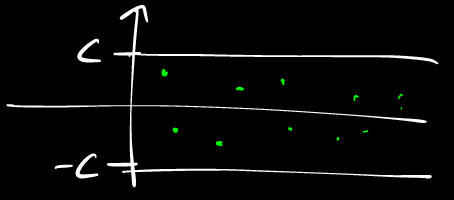
\includegraphics[width=0.9\textwidth]{./media/sequence-bounded}\\~\\
 \includegraphics[width=0.9\textwidth]{./media/sequence-cauchy}
 	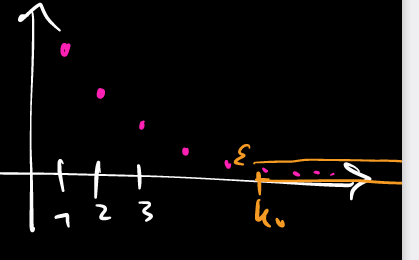
\includegraphics[width=0.9\textwidth]{./media/sequence-null}
\end{minipage}

\end{defi}
\end{frame}
%
\begin{frame}
% BOUNDED SEQUENCES
\begin{ex}
	\blank 
	Let $a\in\R$. The following sequences are bounded:\\


		i) The constant sequence $\{a\}_{k\in\N}$ (choose $C = a$), \\
		
		ii) The sequence $\{\frac{1}{k}\}_{k\in\N}$ (choose $C = 1$),\\
		
		iii) The \textbf{alternating sequence} $\{a (-1)^k\}_{k\in\N}$ (choose $C=a$). This sequence is not convergent but bounded.

~\\
	An example of an unbounded sequence is given by\\
	
	iv) the sequence $\{k^2\}_{k\in\N}$. \\~\\
%	One can show for a sequence $(x^k)_{k\in \N}$ in $\R$:
%	$$(x^k)_{k\in \N}~\text{convergent}~\Rightarrow~(x^k)_{k\in \N}~\text{Cauchy}~\Rightarrow~(x^k)_{k\in \N}~\text{bounded}.$$
\end{ex}
\end{frame}


\begin{frame} 
\begin{theo}[Uniqueness of limits]
	Let $(x^k)_{k\in \N}$ be a sequence in $\R$, then $(x^k)_{k\in \N}$ has at most one limit.
\end{theo}
\begin{proof} \blank
	We proof the statement by contradiction. Therefore, let us assume $(x^k)_{k\in \N}$ converges to $\bar{x}_1$ and $\bar{x}_2$, with $\bar{x}_1\neq \bar{x}_2$. We define $\varepsilon := \frac{1}{2}|\bar{x}_1- \bar{x}_2|>0$. Then by definition of the limit there exist $N_1\in\N$ and $N_2\in\N$ so that
	$$|x^k-\bar{x}_1| <  \varepsilon~~\text{and}~~|x^k-\bar{x}_2| <  \varepsilon$$
	for all $k \geq \max\{N_1,N_2\}$. Thus, by triangle inequality it follows
	$$2\varepsilon= |\bar{x}_1- \bar{x}_2| =  |\bar{x}_1- (x^k-x^k) -\bar{x}_2| \leq |\bar{x}_1-  x^k|+|x^k- \bar{x}_2| < 2\varepsilon.$$
	Since $2\varepsilon< 2\varepsilon$ is a contraction for $\varepsilon>0$, we have that there cannot exist two distinct limits $\bar{x}_1$ and $\bar{x}_2$ as assumed above.
\end{proof}
~\\~\\
Important relation between the different types of sequences:
\begin{theo}\label{theo:relation_conv_cauchy_bound}
	Let $(x^k)_{k\in \N}$ be a sequence in $\R$, then 
	$$(x^k)_{k\in \N}~\text{convergent}~\Rightarrow~(x^k)_{k\in \N}~\text{Cauchy}~\Rightarrow~(x^k)_{k\in \N}~\text{bounded}.$$
\end{theo}\vspace{0.4cm}
\begin{proof}\blank
	We only prove the first implication (the second implication requires some more technical steps). For this purpose let $\tilde{\varepsilon} > 0$. Since $(x^k)_{k\in \N}$ is a convergent sequence, there exists a $\bar{x}\in \R$ and a $k_0 \in \N$, so that
	$$|x^m-\bar{x}| <  \tilde{\varepsilon} ~~\text{and}~~|x^n-\bar{x}| <  \tilde{\varepsilon}$$
	for all $m,n \geq k_0$. Thus, by triangle inequality it follows that
	$$|x^m-x^n| = |x^m-(\bar{x}-\bar{x})+x^n| \leq |x^m-\bar{x}| + |x^n-\bar{x}| < 2\tilde{\varepsilon}.$$ Consequently, for $\varepsilon:= {\tilde{\varepsilon}}/{2}$ we can choose the same $k_0$ to show the Cauchy property.\\
\end{proof} 
\begin{re}
	Note that by definition, in the ordered field $\R$ all Cauchy sequences also converge. However, this is not true in general! For example, we have seen that the sequence produced by Heron's method does not converge in the ordered field $\Q$, i.e., there is no limit point in $\Q$.
\end{re}
\textbf{Remark:} In $\R$ all Cauchy sequences also converge (by definition).
\vspace{2.4cm}
\begin{ex}
	\blank
	sequences that are bounded but not cauchy, cauchy but not convergent
\end{ex}
 \end{frame}


%
\begin{frame} 
%
% SUMS AND PRODUCTS OF SEQUENCES
An important tool to compute limits in practice is the following:
\begin{theo}[Sums and products of sequences]
	Let $(x^k)_{k\in \N}$ and $(y^k)_{k\in \N}$ be two sequences in $\R$ with $\lim\limits_{k\to\infty}x^k= \bar{x}$ and $\lim\limits_{k\to\infty}y^k= \bar{y}$. Then
	\begin{itemize}
		\item[i)] $\lim\limits_{k\to\infty} (x^k + y^k) = \lim\limits_{k\to\infty}x^k + \lim\limits_{k\to\infty}x^k = \bar{x}+\bar{y}$;
		\item[ii)] $\lim\limits_{k\to\infty} (x^k\cdot y^k) = \lim\limits_{k\to\infty}x^k \cdot \lim\limits_{k\to\infty}y^k = \bar{x}\cdot\bar{y}$.
	\end{itemize}
	In particular we find for $a \in \R$ that $\lim\limits_{k\to\infty} (x^k + a) = \bar{x} +a$ and $\lim\limits_{k\to\infty} (x^k \cdot a) = \bar{x}\cdot a$ .
\end{theo} 
\begin{proof} \footnotesize
	i) We define $z^k := x^k + y^k$ and $\bar{z} := \bar{x} + \bar{y}$. Let $\varepsilon>0$. For ${\tilde{\varepsilon}} := \varepsilon/{2}$ there exists a $k_0 \in \N$, so that
	$$|x^k-\bar{x}| <  \tilde{\varepsilon} ~~\text{and}~~|y^k-\bar{y}| <  \tilde{\varepsilon}$$
	for all $k \geq k_0$. Thus by triangle equality we find
	\begin{align*}
	|z^k - \bar{z}| &= |x^k+y^k - (\bar{x} + \bar{y})| 
	= |x^k- \bar{x} +y^k - \bar{y}| 
	\leq |x^k- \bar{x}| + |y^k - \bar{y}| \\
	&<  \tilde{\varepsilon}+\tilde{\varepsilon} = \varepsilon.
	\end{align*}

		ii) We define $z^k := x^k \cdot y^k$ and $\bar{z} := \bar{x} \cdot \bar{y}$. First note that by Theorem \ref{theo:relation_conv_cauchy_bound}, we have that the sequence $(x^k)_{k\in \N}$ is bounded, which implies that there exists a bound $C>0$ so that $|x^k| < C$ for all $k\in\N$. By triangle inequality, we find
	\begin{equation} \label{aux1}
	\begin{aligned}
	|z^k - \bar{z}| &= |x^ky^k -  \bar{x}\bar{y}| 
	= |x^ky^k - (x^k\bar{y}-x^k\bar{y}) + \bar{x}\bar{y}| 
	= |x^k(y^k-\bar{y}) +  (x^k-\bar{x})\bar{y}| \\ 
	&\leq  |x^k(y^k-\bar{y})| +  |( \bar{x}-x^k)\bar{y}| 
	=  |x^k ||(y^k-\bar{y})| +  |( \bar{x}-x^k)||\bar{y}| 
	\leq C |(y^k-\bar{y})| + |( \bar{x}-x^k)||\bar{y}|.
	\end{aligned}
	\end{equation}
	Now let $\varepsilon> 0$. Then for $\tilde{\varepsilon} := \varepsilon/ (C+|\bar{y}|) > 0$ there exists a $k_0 \in \N$, so that 
	$$|x^k-\bar{x}| <  \tilde{\varepsilon} ~~\text{and}~~|y^k-\bar{y}| <  \tilde{\varepsilon}$$
	for all $k \geq k_0$. Thus, combining this with \eqref{aux1} 
	gives the desired result
	\begin{align*}
	|z^k - \bar{z}|  < C \tilde{\varepsilon}  + \tilde{\varepsilon} |\bar{y}| = (C+|\bar{y}|)\tilde{\varepsilon}  = \varepsilon.
	\end{align*}
\end{proof}
 \end{frame}

\begin{frame}
	\begin{ex}
		\blank Let $a \in \R$.
		\begin{itemize}
			\item[i)] The sequence $\{a + \frac{1}{k}\}_{k\in\N}$
			\item[ii)] The sequence $\{a \cdot\frac{1}{k}\}_{k\in\N}$
			\item[iii)] The sequence $\{ \frac{1}{k^2}\}_{k\in\N}$
		\end{itemize}
	\end{ex}
\end{frame}

 
\begin{frame} 
% SQUEEZE THEOREM
~\\[-15pt]
\begin{theo}[Squeeze theorem]
	Let $(x^k)_{k\in \N}$, $(y^k)_{k\in \N}$ and $\{z^k\}_{k\in \N}$ be sequences in $\R$ with $\lim\limits_{k\to\infty}x^k= \bar{x}$ and $\lim\limits_{k\to\infty}z^k= \bar{x}$. If 
	$$x^k \leq y^k \leq z^k~~~\text{for all}~~~k\in\N,$$
	then also
	$$\lim\limits_{k\to\infty}y^k= \bar{x}.$$
\end{theo}
\begin{proof}\blank
	Let $\varepsilon> 0$, then there exists a $k_0 \in \N$, so that, for all $k \geq k_0$,
	$$|x^k-\bar{x}| <  \tilde{\varepsilon} ~~\text{and}~~|z^k-\bar{y}| <  \tilde{\varepsilon}.$$
	Thus, by definition of the absolute value and the assumptions, we find, for all $k \geq k_0$,
	$$-\varepsilon< x^k-\bar{x} \leq y^k-\bar{x} \leq z^k- \bar{x} < \varepsilon.$$
	This implies $|y^k - \bar{x}|< \varepsilon$ for all $k \geq k_0$.
\end{proof}
 \end{frame}
\begin{frame} 
% BUNCH OF EXAMPLES
\begin{ex}
	Let $f\colon \N \to \N$ with $f(k) \geq 0$ for all $k \in \N$. Then the sequence $\{\frac{1}{k + f(k)}\}_{k\in \N}$ is a null sequence.
\end{ex}
 \end{frame}



%%%%%%%%%%%%%%%%%%%%%%%%%%%%%%%%%
% Quadratic equations and inequalities

\begin{frame} 
\Subsection{Quadratic equations and completion of the square}
We want to solve quadratic equations of the following kind
\begin{align} \label{normalform_quadeq}
x^2 + px +q = 0, 
\end{align}
where $p,q\in \R$ are fixed. Representation \eqref{normalform_quadeq} is sometimes referred to as {\color{defgruen} \textbf{normalized form}} or {\color{defgruen} \textbf{reduced form}}.\\
~\\
Recall the binomial formulas: For $a,b \in \R$ we have
\begin{itemize}
	\item[i)] $(a+b)^2 = a^2 + 2ab + b^2$ 
	\item[ii)] $(a-b)^2 = a^2 - 2ab + b^2$ 
	\item[iii)] $(a+b)(a-b) = a^2 - b^2$ 
\end{itemize}
\vspace{0.3cm}
\end{frame}


\begin{frame} 
\begin{ex}
	We want to find all $x \in \R$, that satisfy the quadratic equation $$x^2 + 6x + 5 = 0 .$$
\end{ex}

 \end{frame}

\begin{frame} 
In general we find:\\[4pt]
{\color{satzrot} 
	If $\left(\frac{p}{2}\right)^2 \geq q$, then the quadratic equation
	$$  x^2 + px +q = 0 $$
	is solved by
	$$x = -\frac{p}{2} \pm \sqrt{ \left(\frac{p}{2}\right)^2 - q}.$$
}
\begin{proof}
	\blank
\end{proof}
 \end{frame}


%ALTERNATIVE 1
\begin{frame} 
\textbf{Alternative representation (I)}\\[6pt]
Quadratic equations are also often introduced in the following form:
\begin{align} \label{genform_quadeq}
ax^2 + bx + c = 0 
\end{align}
for fixed $a,b,c \in \R$. Representation \eqref{genform_quadeq} is referred to as the {\color{defgruen} \textbf{general form}} of a quadratic equation.\\[5pt]
Assumed $a \neq 0$ we can deduce the reduced form \eqref{normalform_quadeq}:

 \end{frame}

\begin{frame} 
\begin{ex}
	We want to find all $x \in \R$, that satisfy the quadratic equation $$2x^2 + 8x + 6.72 = 0 .$$
\end{ex}
 \end{frame}


%ALTERNATIVE 2
\begin{frame} 
\textbf{Alternative representation (II)}\\[6pt]
Quadratic equations are also introduced as:
\begin{align} \label{vertexform_quadeq}
a(x-h)^2 + k = 0 
\end{align}
for fixed $a,h,k \in \R$. Representation \eqref{vertexform_quadeq} is referred to as {\color{defgruen} \textbf{vertex form}}.\\[5pt]
Again, we can deduce the reduced form:
 \end{frame}





\begin{frame} 
\textbf{Summary}
 \end{frame}

%%%%%%%%%%%%%%%%
\begin{frame} 
\Subsection{Inequalities}
Here we make use of the fact that $\R$ is an ordered field. In particular we will exploit the \textbf{monotonicity} property:\\[6pt]
Let $a,b\in \R$ with $a\leq b$. Then
\begin{itemize}
	\item[1)] $\forall c\in \R\colon ~ a+c\leq b+c$;
	\item[2)] $\forall c\geq 0\colon ~ ac\leq bc$.
\end{itemize}
From 1) and 2) it follows that
$$\forall c< 0\colon ~ ac\geq bc $$
 \end{frame}


\begin{frame} 
\begin{ex}
	We want to find all $x \in \R$, that satisfy the inequality $$x^2 + 6x + 5 \geq 0 .$$
\end{ex}
 \end{frame}



\begin{frame} 
\begin{ex}
	We want to find all $x \in \R$, that satisfy the inequality $$2x \geq 5x-6.$$
\end{ex}
 \end{frame}


\begin{frame} 
\begin{ex}
	We want to find all $x \in \R$, that satisfy the inequality $$\frac{x+4}{4x-12}  \leq 2.$$
\end{ex}
 \end{frame}



% linalg
\only<presentation>{\setnextsection{1}}
\lecture{Fundamentals of Linear Algebra}{la}
% !TeX spellcheck = en_US
% Recommended reading:
\begin{frame}
	Recommended reading for this section:
	\begin{itemize}
		\item Lectures 1,2,3 in \cite{TreBau}
		\item Sections I.1, I.2, I.3, I.5(, I.11) in \cite{StrangData}
		\item Chapters 1,3(,4,5) in \cite{StrangLA_intro}
	\end{itemize}
	
	\bibliographystyle{plain}
	~\\~\\
	Literature:\\
	\bibliography{../information/literature.bib}
\end{frame}


\begin{frame}
\Vspace{0.2cm}
\Section{Fundamentals of Linear Algebra}
\Subsection{Matrices and Vectors}
\begin{example}[Interpolation] \label{ex:interpolation}
	 ~\\
	Assume we are given the following measurements
	\begin{table}
		\begin{tabular}{c|ccc}
			$z_i$ &-1&0&1\\
			\hline
			$y_i$  &0&1&0
		\end{tabular}
	\end{table}
	We postulate that these measurements can be explained exactly by the (quadratic) model
	$$f(z):=f_{x}(z) := x_1 + x_2 z^2 .$$
	Question: Can we find parameters $x_1,x_2 \in \R$, so that $f(z_i) = y_i$ for all $i=1,\ldots,3$?\\~\\
	\Hide{
		We first translate the task into the following system of \textit{linear} equations:
		\begin{equation*}
		\begin{array}{crcl}
	i=1:	&1x_1 + 1x_2 &=&0\\
	i=2:	&1x_1 +0x_2 &=&1\\
	i=3:	&1x_1 +1x_2 &=&0
		\end{array}
		\ \Leftrightarrow: \
		\underbrace{
			\begin{pmatrix}
			1 & 1 \\ 
			1& 0  \\ 
			1 & 1 
			\end{pmatrix}
		}_{A}
		\cdot
		\underbrace{
			\begin{pmatrix}
			x_1 \\ x_2  
			\end{pmatrix}
		}_{x}
		=
		\underbrace{
			\begin{pmatrix}
			0\\ 1 \\ 0
			\end{pmatrix}
		}_{b}
		\ \Leftrightarrow \
		Ax=b
		\end{equation*}
		Why linear? Roughly speaking, because the $x_i$ only appear with power $1$ and there are no combinations $x_ix_j$.\\~\\
		Also note, the abstracting notation $Ax=b$ provides a rigorous interface to analyze this problem theoretically and also to implement numerical solvers. ~\\~\\
		\demo{solve and draw points}
	} 
\end{example}
\end{frame}


\begin{frame} 
Throughout we will consider matrices over  $\F \in \{\R,\C\}$. However, $\F$ could be replaced by any \href{https://en.wikipedia.org/wiki/Field_(mathematics)}{field}.\\
\begin{defi}[Matrix] \label{def:matrix} 
	\unitlength1cm 
	\begin{picture}(15,0) 
%	\put(10,-3){\includegraphics{LocalFolder/LocalMedia/3_a-indices}} 
	\end{picture} 
	Let $m,n \in \mathbb{N}$. Then a rectangular array of numbers in $\F $ with $m$ \textit{rows} and $n$ \textit{columns}, written as
%	$A: \{1,\ldots, m\} \times \{1, \ldots, n\} \to \F$ represented by the array 
	\begin{eqnarray*} 
		A= (a_{ij})_{ij} = \left(  \begin{array}{cccc} 
			a_{11} & a_{12} & \cdots & a_{1n} \\ 
			a_{21} & a_{22} & \cdots & a_{2n} \\ 
			\vdots & \vdots &        & \vdots \\ 
			a_{m1} & a_{m2} & \cdots & a_{mn} \end{array} \right),
	\end{eqnarray*} 
%	with $a_{ij} \in \F$ for all $i=1,...,m$, $j=1,...,n$
	 is called a  
	{\bf $(m\times n)$ matrix} {\bf with coefficients in $\F$}. \\[4pt]
	\vspace{0.2cm} 
	\Hide{\small
		\begin{tabular}{@{}ll} 
			$\F^{m\times n}$: & set of all $(m\times n)$ matrices with coefficients in  $\F$ \\[0.1cm] 
			$\F^{n} := \F^{n\times 1}$: &matrices with just one column are called (column) \textbf{``vectors''};\\ 
			&elements in $\F^{1\times n}$ are referred to as row vectors \\[0.1cm] 
			$a_{ij}$:        & the $(i,j)$-th {\bf coefficient} or {\bf 
				entry} \\[0.1cm] 
			$(a_{i1},...,a_{in})$: & the $i$-th {\bf row} of $A$ (this is a  
			$(1\times n)$-matrix, , $n$-dimensional vector) \\[0.4cm] 
			$\begin{pmatrix}  a_{1j} \\ \vdots \\ a_{mj}  
			\end{pmatrix}:$ 
			& the $j$-th {\bf column} of $A$ (this is a $(m\times 1)$-matrix, $m$-dimensional vector)
			\\[0.8cm] 
			$0$: & the {\bf zero matrix} or {\bf null matrix}, i.e. all entries $0$ \\[0.1cm] 
			$I_n$: & the  \textbf{unity} or \textbf{identity matrix} in $\F^{n\times n}$, i.e. the Matrix with 
			entries \\ 
			& $\delta_{ij} = \begin{cases} 1, \quad\text{ if }i=j \\ 0, \quad \text{ else} 
			\end{cases}$ ({\footnotesize ``Kronecker delta''}), \quad\text{i.e.}\quad $I_n = \begin{pmatrix} 
			1 & 0 & \cdots & 0\\ 
			0 & & \ddots & \vdots \\ 
			\vdots & \ddots & \ddots & 0 \\ 
			0 & \cdots & 0 & 1  
			\end{pmatrix}$ 
		\end{tabular} 
	}
\end{defi} 
\end{frame}


%OPERATIONS with matrices
\begin{frame}
 \textbf{Operations}~\\
% 
We can add  matrices of same size and scale the entries of a matrix.\\
\Hide{~\\
\begin{ex}[Summing and scaling matrices]
	\begin{align*}
	\begin{pmatrix}2&1\\0&-1\end{pmatrix}
	&+\begin{pmatrix}1&-1\\1&0\end{pmatrix} 
	:=\begin{pmatrix}3&0\\1&-1\end{pmatrix}\\
	2\cdot\begin{pmatrix}2&1\\0&-1\end{pmatrix} 
	&=\begin{pmatrix}2\cdot2&2\cdot1\\2\cdot0&2\cdot(-1)\end{pmatrix}
	:=\begin{pmatrix}4&2\\0&-2\end{pmatrix}
	\end{align*}
\end{ex}
}
%	
\begin{defi}[Summing and scaling matrices]\label{def:sum_scale_mats}
	Let $A,B\in\F^{m\times n}$ be matrices, $m,n \in \N$ and $r \in \F$.
	\vspace{0.2cm}
	\begin{itemize}
		\item[i)] \textbf{Sum of matrices:} $+\colon \F^{m\times n} \times \F^{m\times n} \to \F^{m\times n}$\\ \vspace{0.1cm}
		The sum $C := A + B$ of the two matrices $A$ and $B$ is defined to be the matrix $C= (c_{ij})_{ij} \in \F^{m\times n}$ with entries
		\[
		c_{ij} := a_{ij} + b_{ij}\text{~~~for~~~}i=1,...,m,~ j=1,...,n .
		\]
		\vspace{0.2cm}
		\item[ii)] \textbf{Multiplication with scalars:} $\cdot\colon \F  \times \F^{m\times n} \to \F^{m\times n}$\\ \vspace{0.1cm}
		The product of the matrix $A$ with $r\in\F $ is defined to be the scaled matrix $$r\cdot A := (r\cdot a_{ij})_{ij}.$$
		In this context, elements of the field $\F $ are called \textbf{scalars}.
	\end{itemize}
\end{defi}
\end{frame}



%EXAMPLE: sum and product of matrices
\mode<article>{
\begin{frame} 
\begin{re}~\\
-- why did we need a field $\F $?\\
-- think of $+\colon \F^{m\times n} \times \F^{m\times n} \to \F^{m\times n}$ being an operation on $\F^{m\times n}$\\
Then Because of the entrywise definition, the matrix sum inherits group properties $(G,+)$ from the field $\F $. \\
-- scalar = element of $\F $, think of $\R$
\end{re}

\begin{ex}
\end{ex}
\end{frame}
}



\begin{frame}
	\Hide{\small
\textbf{Question:} How do summing and scaling get along in a mixed expression?\\
We can prove the following rules:\\
\begin{lemma}[Compatibility properties of summing and scaling] \label{lem:compatibility_sum_scale}
	Let $A,B \in \F^{m\times n}$ and $r,s \in \F $. Then 
	\begin{eqnarray*} 
		\begin{array}{lr@{~}l} 
			i) & (r\cdot s) \cdot A = & r\cdot(s\cdot A)  \hspace*{10cm} \\ 
			ii) & (r+s) \cdot A =      & r\cdot A+s\cdot A  \\ 
			~ & r\cdot (A+B) =       & r \cdot A+r \cdot B  \\ 
			iii) & 1\cdot A = & A  
		\end{array}  
	\end{eqnarray*}
\end{lemma}
%
\begin{proof}\blank
	Follow immediately from Definition \ref{def:sum_scale_mats} in terms of matrix coefficients and the field properties of $\F $. For example:
	\begin{itemize}
		\item[i)] $(r\cdot s)A = [(r\cdot s) a_{ij}]_{ij} \stackrel{{(\tiny \text{associativity in} \F)}}{=} [ r\cdot (s \cdot a_{ij})]_{ij} = r \cdot (s\cdot A)$
		\item[ii)]$(r + s)A = [(r + s) a_{ij}]_{ij} \stackrel{{(\tiny \text{distributivity in} \F)}}{=} [ ra_{ij} + sa_{ij}  ]_{ij} = r\cdot A+s\cdot A$
	\end{itemize} 
\end{proof} 
\begin{re}
	One can show that $(\F^{m\times n}, +)$ is a so--called abelian group. Then the compatibility properties from Lemma \ref{lem:compatibility_sum_scale} imply that $(\Fmn, +,\cdot)$ is a so-called {\color{defgruen} \text{vector space} (over $\F $)}.
\end{re}
~\\
From Lemma \ref{lem:compatibility_sum_scale} we can deduce further properties of $(\Fmn, +,\cdot)$.
\begin{corollary}
	Let $A  \in \F^{m\times n}$ and $r  \in \F $. Then
	\begin{eqnarray*} 
		\begin{array}{lr@{~}l} 
			i)& 0 \cdot A &= 0 \\
			ii)& r \cdot 0 & = 0 \\
			iii)& r\cdot A &= 0 ~~ \Rightarrow r = 0 ~\lor ~A = 0\\ 
			iv) & (-1)\cdot A &=    -A ~~~~~~\text{(i.e., $(-1)\cdot A$ is the additive inverse of $A$)}
		\end{array}  
	\end{eqnarray*}
\end{corollary}
\begin{proof} 
	\blank
	Follows from Lemma \ref{lem:compatibility_sum_scale} and the field properties of $\F $. For example:\\[0.2cm]
	iv) To show: $(-1)\cdot A  + A = 0$. We find 
	$$(-1)\cdot A  + A \stackrel{\text{(L.\ref{lem:compatibility_sum_scale} iii))}}{=} (-1)\cdot A  + 1\cdot  A \stackrel{\text{(L.\ref{lem:compatibility_sum_scale} (ii))}}{=} (-1 + 1)\cdot A = 0\cdot A \stackrel{\text{(i)}}{=} 0. $$
\end{proof}
}
 \end{frame}


\begin{frame} 
Next we provide a notation which enables us to write linear systems of equations in a concise way.\\
We recall from Example \ref{ex:interpolation}:
\begin{equation*}
\begin{array}{rcl}
1x_1 + 1x_2 &=&0\\
1x_1 +0x_2 &=&1\\
1x_1 +1x_2 &=&0
\end{array}
\ \Leftrightarrow: \
\underbrace{
	\begin{pmatrix}
	1 & 1 \\ 
	1& 0  \\ 
	1 & 1 
	\end{pmatrix}
}_{A}
\cdot
\underbrace{
	\begin{pmatrix}
	x_1 \\ x_2  
	\end{pmatrix}
}_{x}
=
\underbrace{
	\begin{pmatrix}
	0\\ 1 \\ 0
	\end{pmatrix}
}_{b}
\ \Leftrightarrow \
Ax=b
\end{equation*}
\begin{defi}[Matrix-Vector Product]
 Let $A \in \F^{m\times n}$ and $x\in \F^n$. Then the \textbf{\color{defgruen} matrix-vector product $b=Ax \in \F^m$} is defined by
\[
b_i=a_{i1}x_1+a_{i2}x_2+\ldots +a_{in}x_n=:\sum\limits_{\ell=1}^na_{i,\ell}x_\ell\, ,\qquad \forall i=1,\ldots, m .
\] 		
\end{defi}
\Hide{
A matrix  $A \in \F^{m\times n}$ can therefore also be considered as a (linear) mapping $$f_A:\F^n \to \F^m, ~~x\mapsto Ax.$$	
	\begin{example}[Matrix-Vector Product]~\\
		Let us consider $\laMatSym=\laMatVal$ with columns $\laVecOneSym=\laVecOneVal$ and $\laVecTwoSym=\laVecTwoVal$. Then
		$$
	\begin{matrix}
	i=1 \\
	i=2 \\
	i=3
	\end{matrix}~~
\laMatVal
	\cdot 
	\begin{pmatrix}
	0.5\\ 3
	\end{pmatrix}
	=  \begin{pmatrix}
	1\cdot0.5+2\cdot3 \\
	2\cdot0.5+0\cdot3 \\
	0\cdot0.5+1\cdot3 \\
	\end{pmatrix}
	= 	\begin{pmatrix}
	6.5\\ 1\\ 3
	\end{pmatrix}.
	$$
\end{example}
}
\end{frame}


% MAT-VEC (1) by rows
\begin{frame}
There are two ways of perceiving the matrix-vector product:\\~\\
\textbf{(1) By rows:} \textit{Used for computations}\\
	$$
\laMatVal
\cdot 
\begin{pmatrix}
x_1\\ x_2
\end{pmatrix}
= 	\begin{pmatrix}
1x_1+2x_2\\ 2x_1+0x_2\\ 0x_1+1x_2
\end{pmatrix}
~~~~~= ~\begin{pmatrix}
\text{\color{defgruen}inner products}\\ \text{of the rows}\\ \text{with}~ (x_1, x_2)
\end{pmatrix}
$$
~\\
$\rightarrow$ This refers to the way of computing the matrix-vector product according to ``\textbf{row $\cdot$ column}''.
~\\\vspace{0.4cm}
We give this type of product of two vectors a special name: \vspace{-0.2cm}
\begin{defi}[Inner product]
	Let $x,y \in \F^n$ be two vectors. Then the (standard) \textbf{inner product of $x$ and $y$} is defined by
	\begin{equation*}
	 (x,y)_2 := \overline{x}  \cdot y := \sum_{i=1}^n \overline{x}_i {y}_i = \overline{x}_1{y}_1 + \cdots +\overline{x}_n{y}_n,
	\end{equation*}
	where $\overline{x_i}$ denotes the complex conjugate.\\
\end{defi}
\Hide{	\small
	\begin{itemize}
		\item 	For real vectors $x,y \in \R^n$  this simplifies to
		\begin{equation*}
		(x,y)_2 = \sum_{i=1}^n x_i y_i = x_1y_1 + \cdots +x_ny_n.
		\end{equation*}
		\item This operations is sometimes also called \textit{scalar} or \textit{dot product}. It is a central operation and we will illuminate some properties later on.
	\end{itemize}
\begin{example}[Inner products] ~\\
	\small	$
	\begin{pmatrix}1\\2\\0\end{pmatrix}
	\cdot \begin{pmatrix}3\\-1\\1\end{pmatrix}
	= 1\cdot3+2\cdot(-1)+0\cdot1 = 1
	$,~~$
	\begin{pmatrix}2+3i\\i\\1\end{pmatrix}
	\cdot \begin{pmatrix}1\\-i\\0\end{pmatrix}
	= (\overline{2+3i})\cdot1+\overline{i}\cdot(-i)+\overline{1}\cdot 0 = 2-3i + i^2 = 1-3i
	$.
\end{example}
}
\end{frame}
\begin{frame}
\textbf{(2) By columns:} \textit{Used for understanding}\\
$$
\laMatVal
\cdot 
\begin{pmatrix}
x_1\\ x_2
\end{pmatrix}
= 	
x_1\laVecOneVal
+
x_2\laVecTwoVal
~~~~~= ~\begin{pmatrix}
\text{\color{defgruen}linear combination}\\ \text{of the columns}\\ a_1, a_2
\end{pmatrix}
$$
~\\
\begin{definition}[Linear combination]
	Let $a_1, \ldots, a_n \in \F^m$, $x\in \Fn$. Then 
	$$ \sum_{i=1}^n x_i a_i = x_1 a_1 + \cdots + x_n a_n =  Ax \in \Fm$$
	is called \textbf{linear combination} of the vectors $a_1, \ldots, a_n$. Here, $A :=[a_1, \ldots,a_n] \in \Fmn$.
\end{definition}
%
\Hide{~\\
\begin{example}[Linear combination]
	~\\
	Let us consider $\F = \R$ and again the vectors $\laVecOneSym:=\laVecOneVal$ and $\laVecTwoSym=\laVecTwoVal$.\\ Then examples of linear combinations are:\\ $\laVecOneSym = 1 \cdot \laVecOneSym + 0 \cdot \laVecTwoSym$,\\ 
	$\laVecTwoSym = 0 \cdot \laVecOneSym + 1 \cdot \laVecTwoSym$, \\
	$\laVecOneSym + \laVecTwoSym = ...$,\\
	.... \\
~\\
\demo{picture}
\end{example}
}
\end{frame}



\begin{frame} 
\textbf{The matrix product}\\
We generalize the \textit{matrix-vector} product above to a \textit{matrix-matrix} product by observing that: 
\begin{center}
	\textit{``A matrix is just a collection of columns (or vectors).''}
\end{center}
Idea:\\
\Hide{
	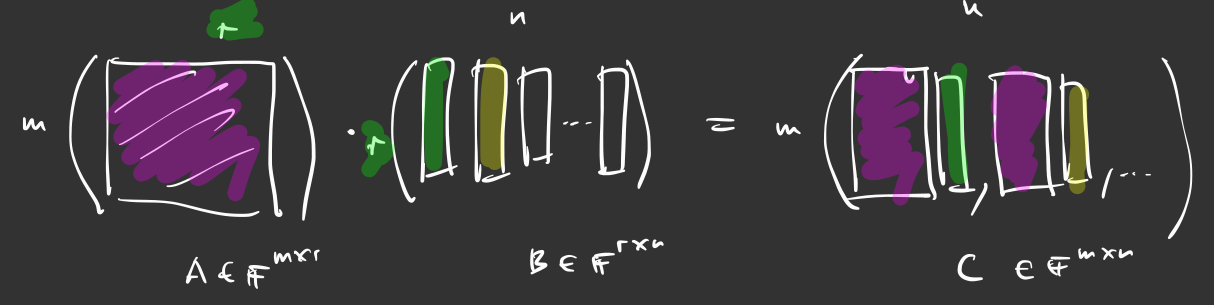
\includegraphics[height=4cm]{media/matrixmatrixproduct}~\\
}
~\\
We make this a rigorous definition:\vspace{-0.25cm}
\begin{defi}[Matrix-Matrix Product] \label{def:mat-mat-product}
	For matrices $A\in\F^{m\times r}$ and $B\in\F^{r\times n}$, we define the {\color{defgruen}\textbf{matrix-matrix product} (or simply matrix product) $C := A\cdot B \in\F^{m\times n}$} as a column wise product, i.e.,
	$$
	\begin{pmatrix}
	{\color{orange}c_{11}}&{\color[rgb]{0.1,0.5,0}c_{12}}&\ldots &{\color{cyan}c_{1n}}\\
	{\color{orange}c_{21}}&{\color[rgb]{0.1,0.5,0}c_{22}}&\ldots &{\color{cyan}c_{2n}}\\
	{\color{orange}\vdots}&{\color[rgb]{0.1,0.5,0}\vdots}&\ddots &{\color{cyan}\vdots}\\
	{\color{orange}c_{m1}}&{\color[rgb]{0.1,0.5,0}c_{m2}}&\ldots &{\color{cyan}c_{mn}}
	\end{pmatrix}
	=\begin{pmatrix}
	a_{11}&a_{12}&\ldots &a_{1r}\\
	a_{21}&a_{22}&\ldots &a_{2r}\\
	\vdots&\vdots&\ddots &\vdots\\
	a_{m1}&a_{m2}&\ldots &a_{mr}
	\end{pmatrix}
	\cdot
	\begin{pmatrix}
	{\color{orange}b_{11}}&{\color[rgb]{0.1,0.5,0}b_{12}}&\ldots &{\color{cyan}b_{1n}}\\
	{\color{orange}b_{21}}&{\color[rgb]{0.1,0.5,0}b_{22}}&\ldots &{\color{cyan}b_{2n}}\\
	{\color{orange}\vdots}&{\color[rgb]{0.1,0.5,0}\vdots}&\ddots &{\color{cyan}\vdots}\\
	{\color{orange}b_{r1}}&{\color[rgb]{0.1,0.5,0}b_{r2}}&\ldots &{\color{cyan}b_{rn}}
	\end{pmatrix}
	\,  ,\text{ i.e. }
	\begin{array}{l}
	\fbox{$\displaystyle c_{ij}=\sum\limits_{{\color{orange}\ell}=1}^ra_{i{\color{orange}\ell}}b_{{\color{orange}\ell} j}$}\\
	i=1,\ldots ,m\\
	j=1,\ldots ,n
	\end{array}
	$$
\end{defi}
\Hide{Note that it is of utmost importance that the matrix dimensions fit in so far as the middle dimension of $A\in\F^{m\times r}, B\in\F^{r\times n}$ (i.e., $r$) is the same. Otherwise, this product cannot be formulated!}
\end{frame}




%% PUT INTO EXERCISE
\begin{frame} 
\Hide{
\textbf{Question:} How do matrix sum (see Def. \ref{def:sum_scale_mats}) and matrix product (see Def. \ref{def:mat-mat-product}) get along in a mixed expression?\\~\\
We can prove the following rules:\\
\begin{lemma}[Compatibility properties of matrix sum and product] \label{lem2.4} 
Let $A,\tilde{A} \in \F^{m\times n}$, $B, \tilde{B} \in \F^{n\times 
l}$, $C \in \F^{l\times t}$, $r \in \F $. Then  
\begin{eqnarray*}
\begin{array}{lr@{~~~}l} 
	(i) & (Associativity) & (A\cdot B) \cdot C = A\cdot (B\cdot C) \hspace*{8cm} \\ 
	(ii) & \mbox{$($Distributivity}\, 1) & (A+\tilde{A})B = AB + \tilde{A} B\\ 
	(iii) & \mbox{$($Distributivity}\, 2) & A(B+\tilde{B}) = AB + A\tilde{B} \\ 
	(iv) & \mbox{(left/right neutral)} & I_m A = AI_n = A \\ 
	(v) & & (r\cdot A)\cdot B  = r(A\cdot B) = A(r\cdot B)\\ 
	(vi) & \mbox{(left/right null)} & 0A = A0 = 0 
\end{array}  \end{eqnarray*} 
\end{lemma} 
\begin{proof}
%
Only a) is not trivial:
$$
[(A\cdot B) \cdot C]_{ij} = \sum\limits_{r=1}^l\left(\sum_{k=1}^n a_{ik}b_{kr}\right)c_{rj}
=\sum_{k=1}^n a_{ik} \left(\sum\limits_{r=1}^lb_{kr}c_{rj}\right)=
[A\cdot (B \cdot C)]_{ij}.
$$  
\end{proof}
}
\end{frame}



\begin{frame}
	\textbf{The (conjugate) Transpose Matrix}\\	~\\
	We finally introduce the operation of transposing matrices (and vectors):
	\begin{defi}[Conjugate Transpose matrix]\label{def:transpose}~\\
		For a matrix $A:=(a_{ij})_{ij}\in\F^{m\times n}$ the \textbf{conjugate (or Hermitian) transpose matrix $A^H$ of $A$} is defined as
		$$A^H:=(\overline{a}_{ji})_{ij}\in\F^{n\times m},$$
		where $\overline{a}_{ji}$ denotes the complex conjugate of the coefficient $a_{ji}$. 
		~\\
		For a real matrix  $A:=(a_{ij})_{ij}\in\R^{m\times n}$, so that $\overline{a}_{ji} = a_{ji}$, this simplifies to 
		$$A^\top := A^H =(a_{ji})_{ij}\in\R^{n\times m}$$
		which we then simply call the \textbf{transpose matrix $A^\top$ of $A$}.
	\end{defi}
\Hide{
	Observe that we have the relation $$A^H = \overline{A}^T, $$
	where $\overline{A}$ is understood as the component-wise complex conjugate.
	~\\
		\begin{example}[Conjugate transpose]~\\
			\begin{itemize}
				\item Transposing a matrix.
				\item Transposing a vector.
				\item The inner product can be written as $x^H y$ (or $x^\top y$ for real vectors).
				\item Adjoint operator: Consider a matrix $A = [a_1, a_2] \in \R^{3 \times 2}$ which maps $\R^2 \to \R^3$. Then $A^\top\in \R^{2 \times 3}$ maps $\R^3 \to \R^2$ and 
				$$A^T p = \begin{pmatrix}
				a_1^\top p\\a_2^\top p
				\end{pmatrix} $$
				collects all inner products of $p$ with the columns. We will relate the inner product to projections later on.
			\end{itemize}
		\end{example}
	}
\end{frame}
 
\begin{frame}
	\Hide{Exercise:\\~\\
	 \textbf{Question:} How do transposing and other matrix operations behave in mixed expressions?\\
~\\
	We can prove the following properties
	\begin{lemma}[Rules for transposing]
		Let $A\in\mathbb{F}^{m\times r}, B\in\mathbb{F}^{r\times m}$ and $r \in \F$. Then
	\begin{enumerate}[i]
		\item[i)] Transposing twice: $(A^H)^H =A$,
		\item[ii)] Matrix product: $(AB)^H=B^H A^H$ ,
		\item[iii)] Scalar product: $(rA)^H= \overline{r} A^H$ ,
		\item[iv)] Matrix sum: $(A+B)^H= A^H + B^H$ ,
		\item[v)] Inverse (see below): For $A\in GL(n,\mathbb{F})$ we have $(A^{H})^{-1}=(A^{-1})^{H}$.
	\end{enumerate}	 
	\end{lemma}
\textbf{Remark:} For real matrices (i.e., $\F=\R$ in the lemma above), the same rules hold true for $(\cdot)^\top$.
\begin{proof}\small
	Apply definitions and exploit properties of $\F$. 
	%TODO
%	Exemplary we show
%		\begin{align*}
%		&C := A \cdot B, C := [c_{ij}]_{ij}, c_{ij} = \sum\limits_{k=1}^n a_{ik}b_{kj}, A^T = [a^\prime_{ij}]_{ij}, B^T = [b^\prime_{ij}]_{ij},\\
%		&[C]_{ij} = C_{ij} = \sum\limits_{k=1}^n a_{jk}b_{ki} = \sum\limits_{k=1}^n a^\prime_{kj}b^\prime_{ik} = \sum\limits_{k=1}^n b^\prime_{ik}a^\prime_{kj} = [B^T A^T]_{ji} \Rightarrow C^T = B^T A^T\\
%		&A \in GL(n, \mathbb{F}), A^{-1}A = I_n \;\; \Rightarrow \;\; \underbrace{(A^{-1}A)^T}_{A^T (A^{-1})^T} = I_n^T = I_n\\
%		&\Rightarrow (A^{-1})^T = (A^T)^{-1}, \text{because Inverse is unique}
%		\end{align*}
\end{proof}

}

\end{frame}

\begin{frame}
\Subsection{Span and Image -- Linear Independence and Kernel }
\Hide{
\begin{example}[Span and Image]\label{ex:span-image}~\\
\textbf{Span:}	Let us again consider the two real vectors
	$$\laVecOneSym=\laVecOneVal,~
	a_2=\begin{pmatrix}2\\0\\1\end{pmatrix}\in\mathbb{R}^3.$$
		Question: What are the vectors that we can represent as linear combination thereof?\\ 
	 There are two operations involved:~\\
	\begin{itemize}
		\item[$\cdot$:]
		Scaling each vector $a_1$ and $a_2$ individually yields infinite lines through these vectors.~\\
		\item[$+$:]
		By adding arbitrary vectors from these lines we fill out the infinite plane in-between.
	\end{itemize}
 All combinations of these two vectors form an infinite plane in $\R^3$. We say the plane is ``spanned'' by $a_1$ and $a_2$. The terminology for the set of all linear combinations is therefore accordingly:
\begin{align*}
\text{span}(a_1,a_2):=
\lbrace x_1\begin{pmatrix}1\\2\\0\end{pmatrix}
+x_2\begin{pmatrix}2\\0\\1\end{pmatrix}
:~x_1,x_2\in\mathbb{R}
\rbrace.
\end{align*}
~\\
\textbf{Image:} By considering these two vectors as columns of a matrix, more precisely,
$$
A=\begin{pmatrix}1&2\\2&0\\0&1\end{pmatrix},
$$
the analogue notion is given by the so-called \textit{image} of the matrix, which collects all matrix--vector products, i.e., 
$$\im(A)~:=\{Ax:~x\in\mathbb{R}^2\}=\lbrace x_1\begin{pmatrix}1\\2\\0\end{pmatrix}
+x_2\begin{pmatrix}2\\0\\1\end{pmatrix}
:~x_1,x_2\in\mathbb{R}\rbrace~=~\text{span}(a_1,a_2).$$
\end{example}
}
\end{frame}
%
\begin{frame}
The set of all possible linear combinations or matrix--vector products is given a special name:
\begin{definition}[Span and Image] \label{def:image-span}~\\
	\begin{itemize}
		\item[i)] The \textbf{span of \underline{vectors} $a_1, \ldots, a_n \in \F^m$} is defined by
		$$ \spann(a_1,\ldots, a_n) :=  \left\lbrace  \sum_{i=1}^n x_i a_i : x_i \in \F \right\rbrace  \subset \Fm.$$
		The set $\{a_1, \ldots, a_n\}$ is called \textbf{generating system} of $\spann(a_1,\ldots, a_n)$.~\\~\\
		\item[ii)] The \textbf{image (or column space) of a \underline{matrix} $A :=[a_1, \ldots,a_n] \in \Fmn$} is defined by
		$$ \im(A) :=  \{Ax:x\in \Fn \} = \spann(a_1,\ldots, a_n) \subset \Fm.$$
	\end{itemize}
\end{definition}
\Hide{~\\
With this terminology we find 
\begin{center}
	``$Ax = b$ is solvable''~~ $\Leftrightarrow$~~ $b$ is spanned by the columns of $A$ ~~$\Leftrightarrow$~~$b \in \im(A)$.
\end{center}
\demo{picture}\\ 
\small
Consider the example from above (i.e., $\laMatSym := [\laVecOneSym, \laVecTwoSym]$) and some vector $b=\laRHSone$. By ``solving'' the system $Ax=b$ we want to find a linear combination of the columns $a_1$ and $a_2$ (i.e., scalars $x_1$ and $x_2$), so that this combination produces the vector $b$, i.e., 
$$Ax=b ~~\Leftrightarrow~~ x_1\cdot\begin{matrix}|\\a_1\\|\end{matrix}
+x_2\cdot\begin{matrix}|\\a_2\\|\end{matrix}=b
~~\Leftrightarrow~~~~x_1\cdot\begin{pmatrix}1\\2\\0\end{pmatrix}
+x_2\cdot\begin{pmatrix}2\\0\\1\end{pmatrix}
=\begin{pmatrix}2\\1\\3\end{pmatrix}.$$
In our example we find that this $b$ is not contained in the span of the columns $a_1, a_2$ (= the infinite plane) so that our system is \textbf{not} solvable.	In particular we find $\im(A) \subsetneqq \R{^3}$ (we say $f_A$ is not ``surjective'').
}\end{frame}	


	


\begin{frame} \small
\Hide{However, what happens if we consider an additional column, e.g.,
$$
A_2 := \begin{pmatrix}
1 & 2 & 3\\ 
2& 0 &2 \\ 
0 & 1 &1
\end{pmatrix} ,~~\text{or}~~~
A_3 := \begin{pmatrix}
1 & 2 & 0\\ 
2& 0 &0 \\ 
0 & 1 &1
\end{pmatrix} .
$$
What is the difference? \\
($A_2$) \textit{Dependent columns:} \\
Here we find that the new column is a linear combination of the first two columns. More precisely,
$$ 	
1\begin{pmatrix}
	1 \\ 2 \\ 0 
\end{pmatrix}
+
1\begin{pmatrix}
	2 \\ 0  \\ 1 
\end{pmatrix} = \begin{pmatrix}
3 \\ 2 \\ 1
\end{pmatrix} \in \im(A).
$$
Therefore, no additional information added to the span: $A_2x=b$ is still not solvable. Furthermore, we easily find a linear combination of the three vectors that yield the zero vector:
$$
1\begin{pmatrix}1\\2\\0\end{pmatrix}+1\begin{pmatrix}2\\0\\1\end{pmatrix}+(-1)\begin{pmatrix}3\\2\\1\end{pmatrix}=\begin{pmatrix}0\\0\\0\end{pmatrix}.
$$
We will later pay special attention to all vectors $x$ for which $Ax = 0$ as here $x:=(1,1,-1)^\top\in~\ker(A_2)$.\\
($A_3$) \textit{Independent columns:}
$$	
x_1\begin{pmatrix}
1 \\ 2 \\ 0 
\end{pmatrix}
+
x_2\begin{pmatrix}
2 \\ 0  \\ 1 
\end{pmatrix}\neq\begin{pmatrix}
0 \\ 0 \\ 1
\end{pmatrix}
 ~~~ \text{for \bf all}~~ x_1, x_2.
$$
Thus, in this case we find
\begin{align*}
x_1\begin{pmatrix}1\\2\\0\end{pmatrix}+x_2\begin{pmatrix}2\\0\\1\end{pmatrix}+x_3\begin{pmatrix}0\\0\\1\end{pmatrix}\stackrel{!}{=}0~~~
\Rightarrow~~x_1=x_2=x_3=0
\end{align*}
We will later understand: $A_3x=b$ is definitely solvable.
}
\end{frame}


\begin{frame}
Let us properly define these concepts:
\begin{definition}[Linear independence and kernel]\label{def:linIndep_Kernel}~\\
	\begin{itemize}
		\item[i)] \underline{Vectors} $a_1, \ldots, a_r \in \F^m$	are called \textbf{linearly independent}, if the only combination that gives the zero vector is $0a_1 + \cdots+0 a_r$.\\
		%In this case, we say that $\spann(a_1,\ldots, a_r)$ has \textbf{dimension} $r$.\vspace{0.2cm}
		\item[ii)] The \textbf{kernel} of a \underline{matrix} $A \in \Fmn$ is defined by $$\ker(A) := \{x\in\Fn: Ax = 0\},$$
		i.e., the preimage of $\{0\}$ under $f_A$. 	
	\end{itemize}
\end{definition}
~\\~\\
 We find the following important equivalent formulation of linear independence:\\
  \begin{lemma} \label{lem:linear-independence}
 	For vectors $a_1,...,a_r \in \Fn$ we have the equivalence:
 	\begin{align*}
 	a_1,...,a_r~~ \text{linearly independent}
 	~~\Leftrightarrow~~
 	&\text{every vector $b \in \text{span} (a_1,...,a_r)$ can be \textbf{uniquely}}\\
 	&\text{linearly combined from the set $\{a_1,...,a_r\}$, i.e.,}\\
 	&\exists_1 x_1,\ldots,x_r \in \F\colon b = x_1a_1 + \ldots +x_ra_r.
 	\end{align*}
 \end{lemma}
 ~\\
\textit{Remark.} This result implies the following for solutions of linear systems: Let $x$ solve $Ax=b$. If $A$ has independent columns, then the solution $x$ is unique! On the contrary, if the columns are dependent, we will learn that there are infinitely many solutions!
\end{frame}

\begin{frame}
	\Hide{
	\begin{proof}[Proof of Lemma \ref{lem:linear-independence} ] 
	Strategy: We split $\mathcal{A} \Leftrightarrow \mathcal{B}$ into $\mathcal{A} \Rightarrow \mathcal{B}$ and  $\mathcal{A}\Leftarrow \mathcal{B}$.
	\begin{itemize}\blank
		\item$\mathcal{A} \Rightarrow \mathcal{B}$: Let $a_1, \cdots a_r$ be linearly independent and $b \in \spann(a_1, \cdots ,a_r)$. To show unique existence, we assume that there exist two instances and show that they are the same. Therefore, let us assume that there are two sets of coefficients, say $x_i$ and $y_i$, so that
		\begin{align*}
			b = \sum\limits_{i=1}^r x_i a_i ~~\text{and}~~ b= \sum\limits_{i=1}^r y_i a_i.
		\end{align*}
		We know that such coefficients exist, since $b \in \spann(a_1, \cdots ,a_r)$ by assumption. Now we find
		\begin{align*}
		& 0 = b-b=\sum\limits_{i=1}^r x_i a_i - \sum\limits_{i=1}^r y_i a_i = \sum\limits_{i=1}^r (x_i - y_i) a_i\\
		&\Rightarrow x_i - y_i =0,\;\text{since}\; a_1, \cdots,a_r \;\text{are linearly independent}\\[10pt]
		&\Rightarrow x_i = y_i , \;\text{i.e., linear combination is unique.}
		\end{align*}
		\item$\mathcal{A} \Leftarrow \mathcal{B}$: We apply a proof by contradiction (i.e., $\neg \mathcal{A} \Rightarrow \neg \mathcal{B} $). For this purpose, we assume $a_1, \cdots, a_r$ are linearly dependent ($\neg \mathcal{A}$), so that there exist ${x_1,\cdots, x_r \in \F}$ with $x_j \neq 0$ for at least one $x_j$, so that
		$$0= \sum\limits_{i=1}^r x_i a_i = \sum\limits_{i=1,i\neq j}^r x_i a_i + x_j a_j.$$
		Since $x_j \neq 0$, we can write $a_j = 0a_1 +\ldots+1a_j+\ldots+0a_r$ also as another linear combination 
		$$ a_j = \sum\limits_{i=1,i \neq j}^r \frac{-x_i}{x_j}a_i =  \frac{-x_1}{x_j}a_1 +\ldots +0 a_j +\ldots  +\frac{-x_r}{x_j}a_r.$$
		Thus the linear dependence ($\neg \mathcal{A}$) applies that there exists a $b \in \spann (a_1,...,a_r)$ (here $a_j$), which is not uniquely linearly combined from $a_1,\ldots, a_r$ ($\neg \mathcal{B}$).
	\end{itemize}
\end{proof}
}
\end{frame}

%\begin{frame}\tiny
%			\textit{deprecated:}\\
%			\begin{lemma} \label{lem:linear-independence}
%				For vectors $v_1,...,v_r \in V$ the following statements are equivalent: 
%				\begin{itemize} 
%					\item[(i)] The $v_1,...,v_r$ are linearly independent.
%					\item[(ii)] every vector $v \in \text{span} (v_1,...,v_r)$ can be uniquely linearly combined from the set 
%					$\{v_1,...,v_r\}$. 
%					\item[(iii)] None of $v_i$ for $ i = 1,\ldots,r$ can be written as a linear combination of the other. 
%				\end{itemize} 
%			\end{lemma}
%			Proof of Lemma \ref{lem:linear-independence}
%			\begin{proof} 
%				Strategy: show (i) $\Rightarrow$ (ii) $\Rightarrow$ (iii) $\Rightarrow$ (i)
%				\begin{itemize}\blank
%					\item[\blank a)] $(i) \Rightarrow (ii)$: $(v_1, \cdots v_r)$ linear independent, let $v \in span(v_1, \cdots ,v_r)$ be combined in two combinations: \begin{align*}
%					&r = \sum\limits_{i=1}^r \lambda_i v_i \;\text{and}\; v= \sum\limits_{i=1}^r \mu_i v_i\\
%					&\Rightarrow 0 = \sum\limits_{i=1}^r \lambda_i v_i - \sum\limits_{i=1}^r \mu_i v_i = v= \sum\limits_{i=1}^r (\lambda_i - \mu_i) v_i\\
%					&\Rightarrow \lambda_i - \mu_i =0,\;\text{since}\; v_1, \cdots,v_r \;\text{are linearly independent}\\[10pt]
%					&\Rightarrow \lambda_i = \mu_i , \;\text{i.e. linear combination is unique}
%					\end{align*}
%					\item[\blank b)] $(ii) \Rightarrow (iii)$: \text{proof by contradiction: assume we have} $a_{ij}$ \text{with} $v_j = \sum\limits_{i=1, i \neq j}^r v_i$\vspace{-0.2cm}
%					\begin{align*}
%					&\text{take}\; \lambda_j := -1 \Rightarrow 0 = \sum\limits_{i=1}^r \lambda_i v_i \;\text{with} \; \lambda_j = -1\\
%					&\text{but also}\; 0 = \sum\limits_{i=1}^r 0\cdot v_i\\
%					&\Rightarrow \;\text{has two different representations as linear combinations of}\; \{v_1,\cdots,v_r\}\hspace{1cm} \lightning (ii)
%					\end{align*} 
%					\item[\blank c)] $(iii) \Rightarrow (i)$: proof by contradiction: assume $v_1, \cdots, v_r$ are linear independent $\Rightarrow \exists{\lambda_i,\cdots, \lambda_r \in \mathbb{F}}$ with $\lambda_j \neq 0$ for at least one $\lambda_j$ with:
%					\begin{align*}
%					&0= \sum\limits_{i=1}^r \lambda_i v_i = \sum\limits_{i=1,i\neq j}^r \lambda_i v_i + \lambda_j v_j\\
%					&\Rightarrow v_j = \sum\limits_{i=1,i \neq j}^r (\frac{-\lambda_i}{\lambda_j})v_i \hspace{1cm} \lightning (iii)
%					\end{align*}
%				\end{itemize}
%			\end{proof}
%		\end{frame}



% SUMMARY
\begin{frame}
	\Hide{
\textbf{Summary:} Relation between vector and matrix notions\\
~\\
	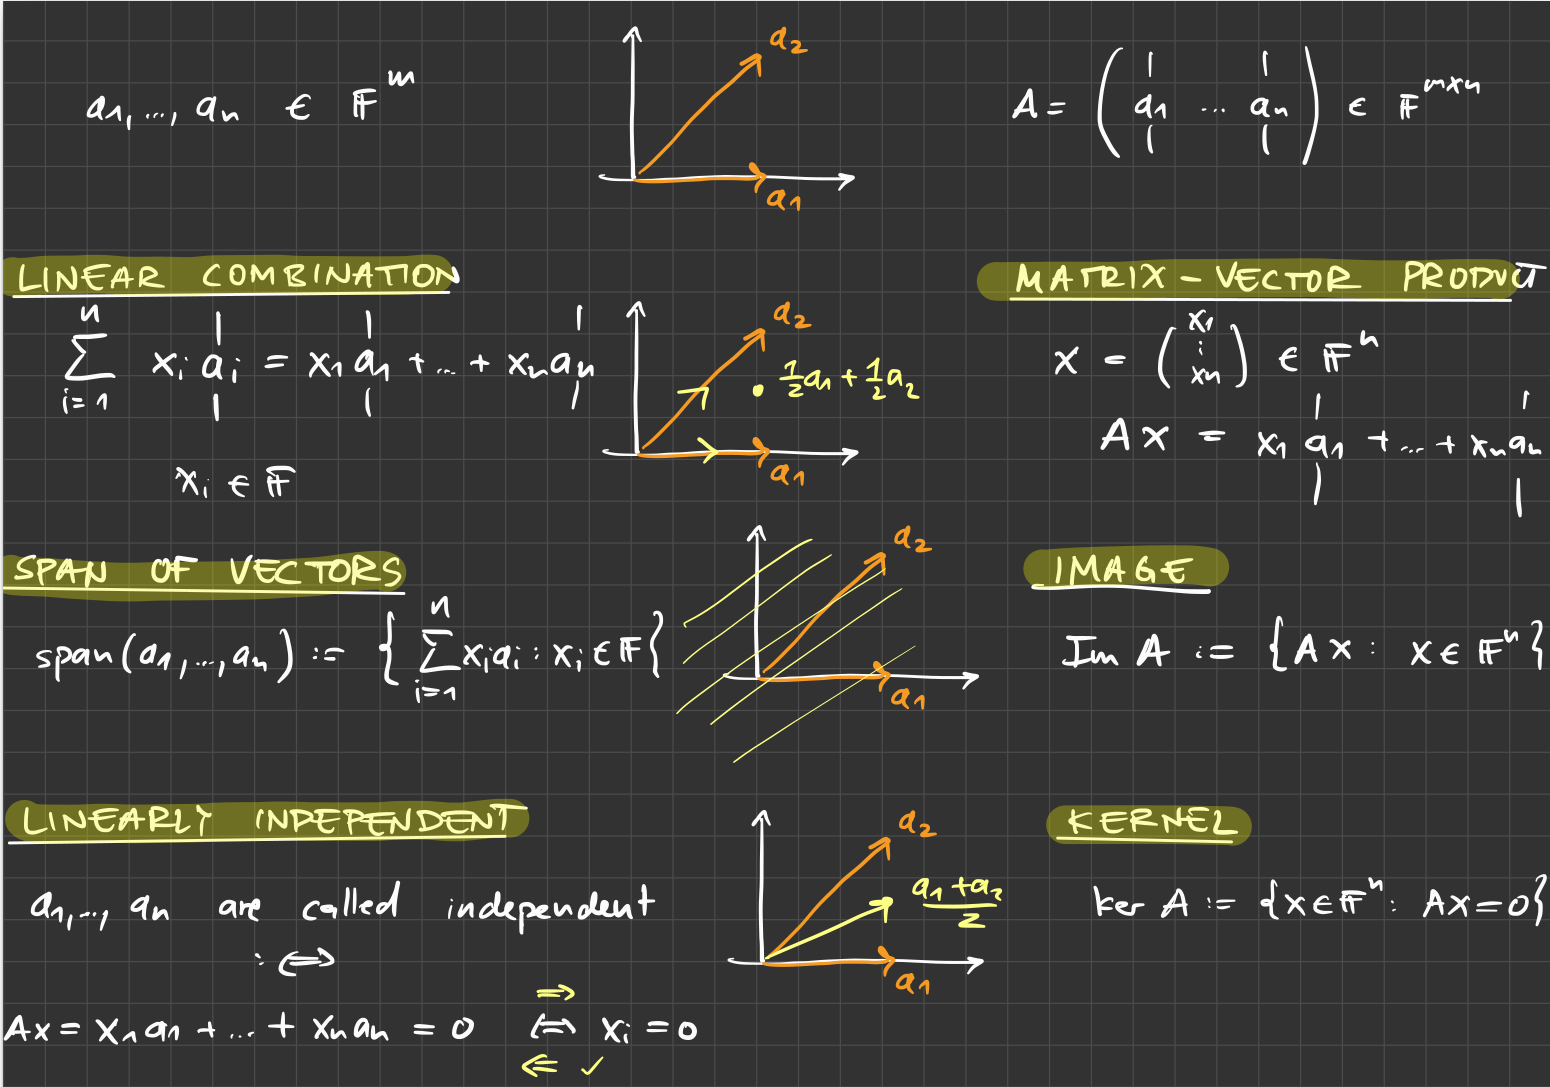
\includegraphics[width=0.9\linewidth]{media/vectorVSmatrix}
}
\end{frame}






%======================
\begin{frame}
\Subsection{Subspaces of $\F^n$ -- Basis and Dimension}
\Hide{
\begin{example}[Subspaces]~\\
	Let $\F = \R$.
	\begin{itemize}
	\item $n=2$: A straight line $L:= \{x a\colon x \in \R\}\subset\R^2$ spanned by a fixed $a\in\R^2$. For a linear function $f(x)=mx$ with $m:=\tfrac{a_2}{a_1}$ we find 
	$$\text{graph}(f)
	:=\{(x,f(x)): x \in \R\} 
	=\{(x,mx): x \in \R\} 
	= \spann(\begin{pmatrix}
	1\\
	\tfrac{a_2}{a_1}
	\end{pmatrix})
	= \spann(\begin{pmatrix}
	  a_1\\
    a_2
	\end{pmatrix})~~~(\text{note:}~ a_1\R = \R) 
	$$
		\item  $n=3$: A plane $P:= \{x_1 a_1+ x_2 a_2\colon x_i \in \R\}\subset \R^3$ spanned by fixed $a_1, a_2\in\R^3$.\\
	\item  Not a (linear) subspace: The graph of nonlinear functions, such as $x^2$ or $\sin(x)$ in $\R^2$.
\end{itemize}
\demo{pictures}
\end{example}
~\\~\\
}

%
\begin{definition}[Subspace] \label{def:subspace}
	A subset $V \subset \F^n$ is called \textbf{(linear) subspace of $\F^n$} if 
	\begin{itemize}
		\item[i)] it is nonempty, i.e., $V\neq \emptyset$,
		\item[ii)] and if it is closed under linear combinations, i.e., if 
		\begin{align*}
		\lambda_1 v_1 + \lambda_2 v_2 \in V ~~~\text{for all}~~~v_1, v_2 \in V,~\lambda_1, \lambda_2 \in \F .
		\end{align*}
	\end{itemize} 
\end{definition}
\end{frame}




\begin{frame}
\textbf{Question:} Is it possible to describe a linear subspace of $\Fn$ by a finite number of vectors?
\begin{definition}[Basis]\label{def:basis}
Let $V \subset \F^n$ be a subspace of $\F^n$. Then a set of vectors $\{v_1, \ldots, v_r\} \subset V$ with $r\leq n$ is called \textbf{basis of $V$}, if 
\begin{itemize}
	\item[i)] $v_1, \ldots, v_r$ are linearly independent,
	\item[ii)] $\text{span}(v_1, \ldots, v_r) = V$.
\end{itemize}
\end{definition}
~\\
\Hide{
		\begin{itemize}\blank
	\item Let $\{v_1, \ldots, v_r\} \subset V$ be a basis. Then, in particular, any $v \in V=\text{span}(v_1, \ldots, v_r)$ can be written as
	\begin{align*}
	v = \sum_{j=1}^r \lambda_j v_j
	\end{align*}
	for some \textit{uniquely} determined scalars $\lambda_j \in \F $ (see Lemma \ref{lem:linear-independence}).\\
	$\rightarrow$ These scalars are called \textbf{\color{defgruen} coordinates} of $v$ with respect to the basis $\{v_1, \ldots, v_r\}$. ~\\~\\
	\item One can show that 
	\begin{itemize} \normalsize
		\item {\color{satzrot}there exists a basis} (general result based on Zorn's lemma),
		\item {\color{satzrot}any basis of a subspace of $\F^n$ has the same length} (doable proof), which we call \textbf{\color{defgruen}dimension of $V$ ($\dim(V)$)}.
	\end{itemize} 
~\\
	\item With other words: 
	\begin{center}
		\textit{The maximum number of linearly independent vectors is called dimension and the set of such vectors is called a basis.}
	\end{center}
\end{itemize}
}
\end{frame}


%%
\begin{frame}
\Hide{ \small
\begin{example} \label{ex:subspaces}
~\\
\textbf{1)} Let us consider $\F =  \R$ and $V:= \mathbb{R}^2\subset \R^2$.\\~\\
We first show that $V$ is a subspace of $\mathbb{R}^2$ and then try to find some bases.~\\
Following Definition \ref{def:subspace} we show:\\
\begin{itemize}
	\item[i)] $V \neq \emptyset$: Consider $0 \in V$.
	\item[ii)] $V$ is closed under linear combinations: Let $v_1, v_2 \in V,~\lambda_1,\lambda_2 \in \R$, then clearly $\lambda_1v_1+\lambda_2v_2 \in \R^2=V$.
\end{itemize}
Now it makes sense to talk about a \textit{basis} for $V$. We next try to find a set of vectors $v_1,\ldots, v_r \in V$ that satisfies Definition \ref{def:basis}.\\

\begin{itemize}
	\item[\textbf{1a)}] Let us consider the vectors $e_j := (\delta_{ij})_{1\leq i \leq n} = (0\ldots 1 \ldots 0)^\top \in \Rn$, here with $n=2$. We show that $\{e_1,e_2\}$ is a basis of $V$ by verifying the two conditions in Definition \ref{def:basis}.
	\begin{itemize}
		\item[i)] We show that $e_1,e_2$ are linearly independent. From
		$$x_1e_1+x_2e_2=\begin{pmatrix}x_1\\x_2\end{pmatrix}\stackrel{!}{=}0$$	
		we easily conclude that $x_1=0=x_2$, so that $e_1,e_2$ are indeed linearly independent.
		\item[ii)] By Definition \ref{def:sum_scale_mats} any $v=\begin{pmatrix}v_1\\v_2\end{pmatrix}\in V=\mathbb{R}^2$ can be written as
		$$v=v_1\begin{pmatrix}1\\0\end{pmatrix}+v_2\begin{pmatrix}0\\1\end{pmatrix} = v_1e_1+v_2e_2.$$
		Thus 
		$$V = \R^2 = \{v_1e_1+v_2e_2 \colon v_1,v_2 \in \R \} =\text{span}(e_1,e_2).$$
	\end{itemize}
In terms of the previous slide, we have that	$v_1,v_2$ are the coordinates of $v$ w.r.t the basis $\{e_1,e_2\}$ and the dimension of $V$ is 2, we write $\dim(V)=2$.\\~\\
	\textit{\textbf{Remark}: Analogue results hold true for any $\R^n$ (not just $n=2$) and the set of vectors $\{e_1,\ldots,e_n\}$ is called the {\color{defgruen}standard basis} or {\color{defgruen}unit vectors in $\Rn$}.}
\end{itemize}
\end{example}
}
\end{frame}

%%
\begin{frame}
	\Hide{\footnotesize 
	\begin{itemize}
		\item[\textbf{1b)}] Let us find another basis for $\R^2$ and check whether its length is still 2 in accordance with the remarks after Definition \ref{def:basis}.\\
		For instance, let us consider the vectors
	$$a_1=\begin{pmatrix}1\\0\end{pmatrix},~a_2=\begin{pmatrix}1\\1\end{pmatrix} \in V.$$
Again, we verify that the two conditions in Definition \ref{def:basis} are satisfied:
\begin{itemize}\footnotesize
	\item[i)] Now let us use the equivalent formulation of linear independence from Lemma \ref{lem:linear-independence}. For this purpose let $v \in \text{span}(a_1,a_2)$ so that there exist scalars $\lambda_1,\lambda_2\in\mathbb{R}$ with
	$$\begin{pmatrix}v_1\\v_2\end{pmatrix} = \lambda_1a_1+\lambda_2a_2,$$
	which, after inserting the precise numbers for $a_1$ and $a_2$, is equivalent to
	$$\begin{pmatrix}\lambda_1\\0\end{pmatrix}
	+\begin{pmatrix}\lambda_2\\\lambda_2\end{pmatrix}
	=\begin{pmatrix}v_1\\v_2\end{pmatrix}.$$
	Using matrix notation we can even write
	$$\begin{pmatrix}
	1&1\\0&1
	\end{pmatrix}\cdot \begin{pmatrix}\lambda_1\\\lambda_2\end{pmatrix} = \begin{pmatrix}v_1\\v_2\end{pmatrix}. $$
	In order to apply Lemma \ref{lem:linear-independence}, we need to show that the scalars $\lambda_1,\lambda_2$ are uniquely determined by this equation. Therefore, let us now solve this upper triangular system (we will later learn about \textit{backward substitution} to do this algorithmically). We observe from the bottom equation that
	$\lambda_2=v_2. $
	Inserting this into the top equation then yields
	$$\lambda_1+\lambda_2=v_1 ~~\Leftrightarrow~~\lambda_1+v_2=v_1~~\Leftrightarrow~~\lambda_1=v_1-v_2.$$
	Observe that $\lambda_1$ and $\lambda_2$ are uniquely determined, i.e., there are no other $\lambda_1$ and $\lambda_2$ solving the upper equations; thus $a_1,a_2$ are independent by Lemma \ref{lem:linear-independence}. Also, let us make a quick test:
	$$(v_1-v_2)a_1+v_2a_2 =\begin{pmatrix}v_1-v_2\\0\end{pmatrix}+\begin{pmatrix}v_2\\v_2\end{pmatrix}
	=\begin{pmatrix}v_1\\v_2\end{pmatrix}. $$
	\item[ii)] We note that $\text{span}(a_1,a_2) \subset \R^2 = V$ is obviously true and to prove the reverse subset relation we choose the scalars $\lambda_1=v_1-v_2,~\lambda_2=v_2$ for $v=(v_1,v_2)^\top \in V=\R^2$.
\end{itemize}
		All in all, we have that $\lambda_1=v_1-v_2,~\lambda_2=v_2$ are the coordinates of $v \in V$ w.r.t the basis $\{a_1,a_2\}$ of $V$ and $\dim(V)=2$. \\
		\Vspace{0.1cm}
		\textit{\textbf{Remark:} The notation for vectors introduced in D. \ref{def:matrix} implicitly assumes that vectors are represented in the standard basis.} 
	\end{itemize}
}
\end{frame}



%
%\begin{frame}
%\begin{theorem}\label{basis-complement} Let $V$ be a vector space over the field $\F $. 
%\ite
%\item[i)] if $V=\text{span}(v_1,\ldots,v_n)$, then any linearly independent set $\{w_1,\ldots,w_r\}\subset V$ ($r<n$), can be complemented by elements from $\{v_1,\ldots,v_n\}$ to a basis of $V$.
%\item[ii)] if $V$ has a finite basis ($n < \infty$), then any basis has the same length, which we call \emph{\color{defgruen} \textbf{dimension}} of $V$.
%\item[iii)] a set $\{v^1,\ldots ,v^n\}\subset \F^n$ is a basis of  
%$\F^n$, if the matrix consisting of these vectors as columns
%\[
%A:=\left[\begin{array}{c@{\quad}c@{\quad}c@{\quad}c}
%v^1 & v^2 & \dots & v^n
%\end{array}\right]
%:=
%\left[\begin{array}{cccc}
%v^1_1 & v^2_1 & \dots & v^n_1\\
%v^1_2 & v^2_2 & \dots & v^n_2\\
%\vdots & \vdots & \dots & \vdots\\
%v^1_n & v^2_n & \dots & v^n_n
%\end{array}\right]
%\]
%is invertible.
%\eti 
%\end{theorem}
%\end{frame}





\begin{frame}
In the exercises we will prove that for any matrix $A \in \Fmn$, the kernel $\ker(A)$ is a subspace of $\Fn$ and the image $\im(A)$ is a subspace of $\Fm$. In the context of matrices these are important spaces and we give their dimensions a special name:\\
\begin{defi}[rank and nullity]\label{def:rank-nullity}
	 Let $A \in \Fmn$. Then
	\begin{itemize}
		\item[-] $\rank(A)  := \dim(\im(A))$ is called the (column) \textbf{rank of $A$},
		\item[-] $\nullity(A) := \dim(\ker(A))$ is called the \textbf{nullity of $A$}.
	\end{itemize}
\end{defi}
\Hide{~\\
\begin{example}\small~\\
	\begin{itemize}
		\item [\textbf{1)}] Let us consider the matrix $A=[a_1,a_2,a_3]:=\begin{pmatrix}
		1&1&2\\0&1&1
		\end{pmatrix} $.\\
		\textbf{1a)} By Definition \ref{def:image-span} of the image we have 
		$\im(A)=\text{span}(a_1,a_2,a_3).$
		By observing $a_3 = a_2 + a_1$, i.e., $a_3$ is a linear combination of $a_1$ and  $a_2$, we even find that $\im(A)~=~\text{span}(a_1,a_2).$
		Since the vectors $a_1, a_2$ have been identified to be linearly independent (see Example \ref{ex:subspaces}), we find by Definition \ref{def:basis} that they form a basis for $\im(A)$. Thus
		$$\rank(A) =  \dim(\im(A))=2.$$
		\textbf{1b)} What about the nullity? We first need to find a basis of the kernel (we will do this by re-writing it as a span of some independent vectors). For this purpose, let $x \in \ker(A)$, which by Definition \ref{def:linIndep_Kernel} is equivalent to
		$$Ax = 0 ~~\Leftrightarrow~~x_1+x_2+2x_3 = 0, ~~x_2+x_3 =0. $$
		Now from the second equation we obtain $x_2 = -x_3$. Let us also write $x_1$ as a function of $x_3$. This is achieved by inserting $x_2 = -x_3$ into the first equation to obtain 
		$$x_1+x_2+2x_3 =x_1-x_3+2x_3  =x_1+x_3=  0 ~~\Leftrightarrow~~x_1 = -x_3.$$
		Thus we find
		$$Ax = 0 ~~\Leftrightarrow~~x = \begin{pmatrix}
		x_1\\x_2\\x_3
		\end{pmatrix}  = \begin{pmatrix}
		-x_3\\-x_3\\x_3
		\end{pmatrix} = x_3\begin{pmatrix}
		-1\\-1\\1
		\end{pmatrix}.$$
	
	\end{itemize}
\end{example}
}
\end{frame}

\begin{frame}
	\Hide{	~\\
\begin{itemize}
	\item[] 		\small	With other words, we can write
		$$\ker(A) = \{\begin{pmatrix}
		x_1\\x_2\\x_3
		\end{pmatrix}\in\R^3\colon x = x_3\begin{pmatrix}
		-1\\-1\\1
		\end{pmatrix} \} = \{x_3\cdot\begin{pmatrix}
		-1\\-1\\1
		\end{pmatrix}\colon x_3 \in \R \} = \text{span}(\begin{pmatrix}
		-1\\-1\\1
		\end{pmatrix}).$$
		Since $\begin{pmatrix}
		-1\\-1\\1
		\end{pmatrix} \neq 0$ it forms an independent set of length 1 so that by Definitions \ref{def:basis} and \ref{def:rank-nullity} we finally conclude that 
		$$\nullity(A) = \dim(\ker(A)) =1. $$
	~\\~\\
	\textit{\textbf{Remark:} We observe that $$\rank(A) + \nullity(A) = 3~~~ \text{(=column dimension)}.$$ We will see below that this is generally true -- called the \textit{dimension formula}!}
\end{itemize}
}
	
\end{frame}


\begin{frame}
\Hide{\small	\begin{itemize}
			\item [\textbf{2)}]	Let us consider $A= [a_1,a_2]:=\begin{pmatrix}
	1&2\\1&2\\0&0
	\end{pmatrix}$.~\\ 
	\textbf{2a)} Since $a_2 = 2\cdot a_1$, the columns are certainly linearly dependent (e.g., $2\cdot a_1+ (-1)a_2 = 0 \in \R^2 $; a combination that yields zero but with nonzero coefficients). Therefore
	$$\im(A) = \text{span}(a_1, a_2) = \text{span}(a_1), $$
	so that $$ \rank(A)=\dim(\im(A)) = 1.$$\\~\\
	\textbf{2b)} Now let us consider the kernel ker$(A) =\{x:~Ax=0\}$. Following along the lines of the previous slides we get
	\begin{align*}
	Ax=0~~&\Leftrightarrow~~\begin{pmatrix}1\\1\\0\end{pmatrix}x_1+\begin{pmatrix}2\\2\\0\end{pmatrix}x_2=\begin{pmatrix}0\\0\\0\end{pmatrix}~~
	\Leftrightarrow~~\begin{pmatrix}x_1+2x_2\\x_1+2x_2\\0\end{pmatrix}=\begin{pmatrix}0\\0\\0\end{pmatrix}
	\Leftrightarrow~~x_1=-2x_2
	\end{align*}
	and thus
	$$	\ker(A)=\{x\in\mathbb{R}^2:~x_1=-2x_2\}
	=\lbrace\begin{pmatrix}-2x_2\\x_2\end{pmatrix}\in\mathbb{R}^2:~x_2\in\mathbb{R}\rbrace
	=\lbrace x_2\begin{pmatrix}-2\\1\end{pmatrix}\in\mathbb{R}^2:~\lambda\in\mathbb{R}\rbrace
	=~\text{span}\left(\begin{pmatrix}-2\\1\end{pmatrix}\right).
$$
So all in all, $\nullity(A) = \dim(\ker(A))  =1$.\\
~\\
\textit{\textbf{Remark:} Again we observe that $$\rank(A) + \nullity(A) = 2~~~ \text{(=column dimension)}.$$}
	\item[\textbf{3)}] Similarly, considering the matrices from above we find $\rank(A_2) = 2$ and  $\rank(A_3) = 3$.
\end{itemize}}
\end{frame}

\begin{frame}

\textbf{Question:} Can we find a general relation between the nullity and the rank of a matrix?

\begin{theorem}[Dimension Formula/Rank--Nullity Theorem] \label{dimension-formula}
	Let $A \in \Fmn$, then 
$$\rank(A) +  \nullity(A) = n. $$
\end{theorem}
\Hide{
~\\
\begin{itemize}
	\item The dimension formula also reads as
$$\dm(\im(A)) + \dm(\kernel(A)) = \dm(\Fn). $$
~\\
\item \textbf{Intuition:}  Let us again think of a matrix $A \in \Fmn$ as a mapping from $\Fn$ to $\Fm$. If the matrix maps some vectors of this $n$--dimensional space $\Fn$ to $0$ -- precisely those vectors from the kernel of A -- then we can say that this ``piece of information'' gets lost. What prevails from $\Fn$ makes up the image of $A$ whose dimension is the rank of the matrix by definition. So, the amount of information in $\Fn$ equals the information that gets lost after mapping it by $A$ ($\nullity(A)$) plus the one that prevails ($\rank(A)$).
~\\
%\item We will later learn about an equivalent rank definition. More precisely, we will find that:\\~\\ \centering
%	{\color{satzrot} rank($A$) = maximum number of linearly independent column vectors.}
\end{itemize}	
}
\end{frame}



\begin{frame}\Subsection{Inverse Matrices}
	\Hide{
\begin{example}[Inverses]\label{ex:inverse}%\small
	Let us consider the following matrix
		$$A=[a_1,a_2]=\begin{pmatrix}1&1\\0&1\end{pmatrix},$$
	which is composed of the vectors considered in Example \ref{ex:subspaces} 1b).\\~\\
	\textit{Recall results Ex.\ref{ex:subspaces} 1b):} We have already observed that $a_1,a_2$ are independent and $\spann(a_1,a_2) = \R^2$. With other words, for any $b\in \R^2$, by Lemma \ref{lem:linear-independence} there exist unique (!) scalars $x_1,x_2$, so that $Ax =x_1 a_1 + x_2a_2=b$. More precisely, for $x_b=\begin{pmatrix}b_1-b_2\\b_2\end{pmatrix}$ (coordinates of $b$ wrt. the basis $\{a_1,a_2\}$) we found
	$$Ax_b=\begin{pmatrix}1&1\\0&1\end{pmatrix}
	\begin{pmatrix}b_1-b_2\\b_2\end{pmatrix}=\begin{pmatrix}b_1\\b_2\end{pmatrix}=b.$$\\~\\
	Clearly, the vector $x_b$ is composed of information from $b$.
	Now let us consider the following mapping
	$$b\mapsto x_b=\begin{pmatrix}b_1-b_2\\b_2\end{pmatrix}=
	\begin{pmatrix}	1\\0\end{pmatrix}b_1 + \begin{pmatrix}	-1\\1\end{pmatrix}b_2
	=\underbrace{\begin{pmatrix}1&-1\\0&1\end{pmatrix}}_{=:A^{-1}}\begin{pmatrix}b_1\\b_2\end{pmatrix}.$$
	We observe that the mapping from the vector $b$ to its coordinates $x_b$ w.r.t. the basis $\{a_1,a_2\}$ can be expressed as a matrix--vector product. The involved matrix $A^{-1}$ is referred to as the \textit{inverse matrix} of $A$.
\end{example}
}
\end{frame}

\begin{frame}
	\textbf{In general:}\\~\\
	Consider the matrix as a mapping $$f_A:\mathbb{F}^n\rightarrow\mathbb{F}^n,~x\mapsto Ax.$$
	Then by definition the \textit{mapping} $f_A$ is \textbf{\color{defgruen}invertible}, if there exists a mapping $f_A^{-1}:\mathbb{F}^n\rightarrow\mathbb{F}^n$ such that for all $x,b \in \mathbb{F}^n$
	we have 
	$$f_A(x)=b~~~\Leftrightarrow~~~x=f_{A}^{-1}(b).$$
	Inserting the definition of $f_A$ this reads as
	$$Ax=b~~\Leftrightarrow~~x=A^{-1}b.$$
	Verifying this condition for all possible $x$ and $b$ would be an ambitious endeavor. Luckily, this condition can be rephrased into conditions solely involving the matrix $A$. More precisely, by inserting one into the other we obtain
	\Hide{~\\
	\begin{itemize}
		\item[i)] $Ax = b  ~~\Leftrightarrow~~ AA^{-1}b=b~~\Leftrightarrow~~AA^{-1}= I $,
		\item[ii)] $x=A^{-1}b  ~~\Leftrightarrow~~ x=A^{-1}Ax ~~\Leftrightarrow~~A^{-1}A= I $.
	\end{itemize} 
~\\
	Let us quickly check this for Example \ref{ex:inverse}:\\
	 ~\\
	 $~~A^{-1}A =\begin{pmatrix}1&-1\\0&1\end{pmatrix}\begin{pmatrix}1&1\\0&1\end{pmatrix}=\begin{pmatrix}1&0\\0&1\end{pmatrix}=I_2 ~~\checkmark$,
	 ~~~  $~~AA^{-1} =\begin{pmatrix}1&1\\0&1\end{pmatrix}\begin{pmatrix}1&-1\\0&1\end{pmatrix}=\begin{pmatrix}1&0\\0&1\end{pmatrix}=I_2~~\checkmark.$


}
\end{frame}



\begin{frame} 
	Let us make this a definition.
	\vspace{0.25cm}
	\begin{defi}[Inverse matrix] \label{def2.5} 
		A matrix $A \in \F^{n\times n}$ is called {\bf invertible}, if there exists 
		a matrix $\tilde{A} \in \F^{n\times n}$ with 
		\begin{equation} \label{eq:definvertible_mat}
		A\cdot\tilde{A}  = \tilde{A}\cdot A=
		I_n.
		\end{equation}
		In case of existence we find that $\tilde{A}$ is unique (see below) and we denote by $A^{-1}:= \tilde{A}$ the {\bf inverse matrix} 
		of $A$. The set of all invertible matrices in $\Fnn$ is denoted by $GL_n (\F )$, the so-called {\em
			general linear group}.   
	\end{defi}
\Hide{
	\vspace{1.25cm}
	Consider the linear equation 
	$$Ax = b$$
	By setting $\color{cyan}x := A^{-1}b$, we find
	$$A {\color{cyan}x} = A {\color{cyan} A^{-1}b} = {\color{red} A A^{-1}}b = {\color{red}I_n}b = b .$$
	~\\
	If $A$ is invertible, then 
	\begin{center}
		``solving $Ax = b$''~~~$=$~~~``{\color{cyan} applying} the {\color{orange} inverse matrix $A^{-1}$}''\\\vspace{0.3cm}
		\hspace{3cm}{\color{cyan} (\textit{numerical methods})}  ~~~~~~~~~~~{\color{orange} (\textit{not accessible in practice})}
	\end{center}
}
\end{frame}






\begin{frame}
	From the dimension formula \ref{dimension-formula} for $n=m$, we find \textbf{``injectivity $=$ surjectivity''}\\~\\
	\Hide{	\pictures{~\\
			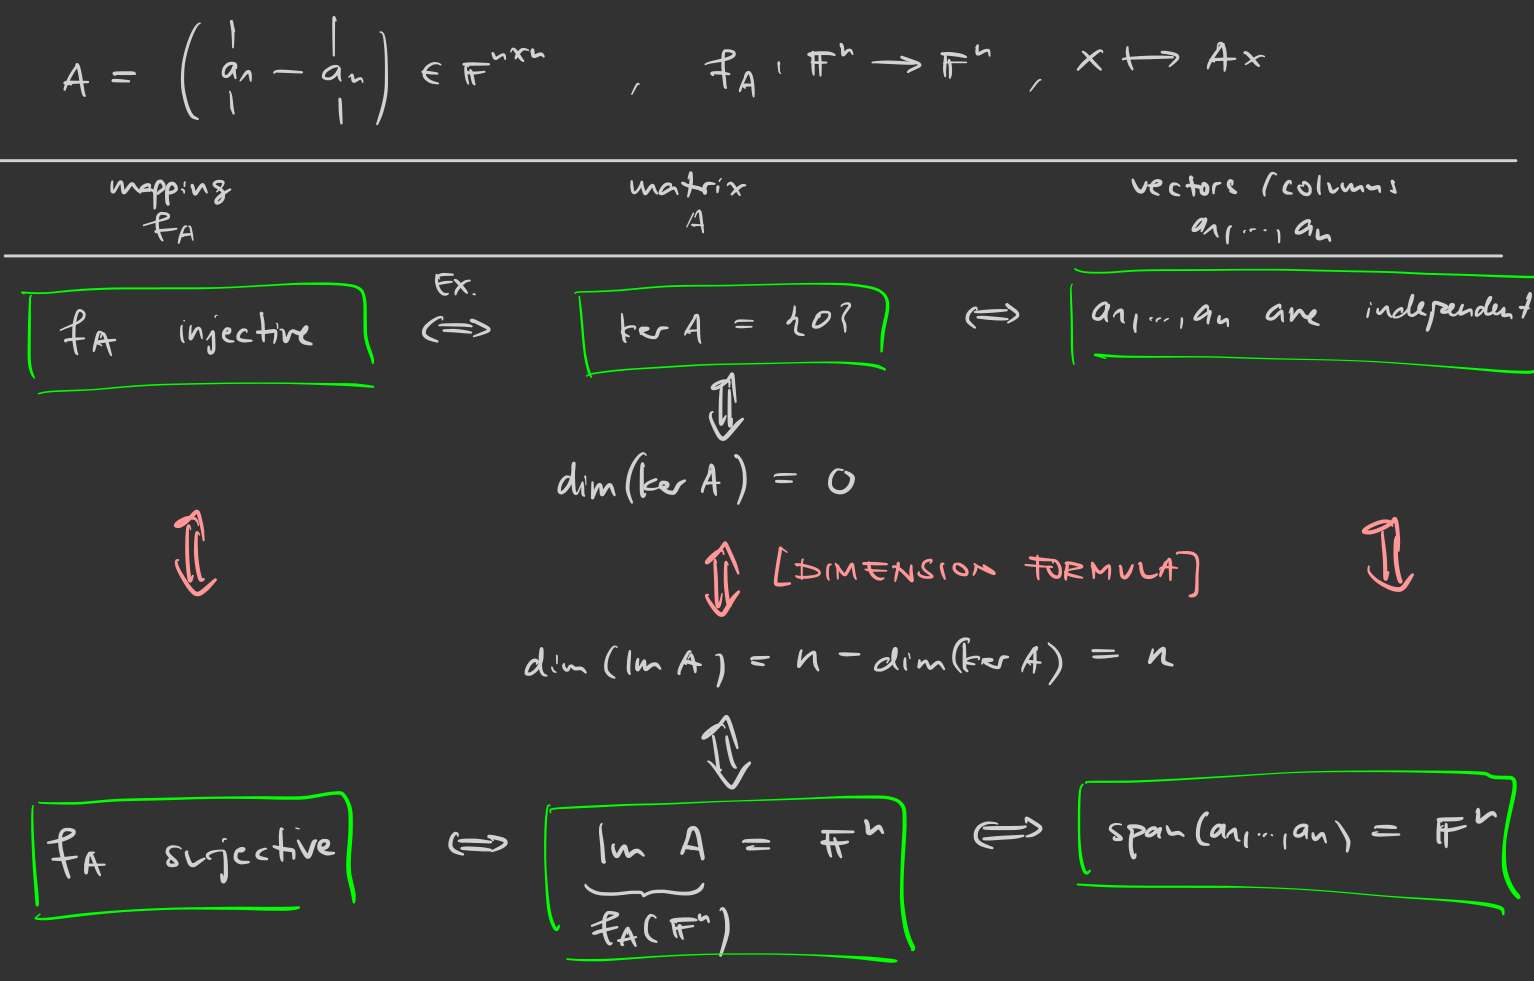
\includegraphics[width=0.9\textwidth]{media/la-InverseMatrices1}}~\\
		~\\Also see Lemma \ref{lem:linear-independence}}
\end{frame}


\begin{frame}
	\textbf{Remark:}\\ A System $Ax = b$ can be solvable even if $A$ is not squared (and thus not invertible)! \\	
~\\
\Hide{\pictures{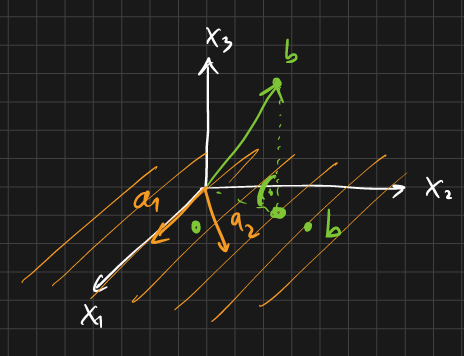
\includegraphics[width=0.17\textwidth]{media/dim-formel}}
	~\\
	The Difference:\vspace{0.2cm}
	\begin{itemize}
				\item \textit{invertible} ($m = n$): For \textbf{any} $b$ there is a \textbf{unique} $x$ so that $Ax = b$, i.e.,\\\vspace{0.2cm} 	
		~~~~~~~~~~~~~~~~~~~~~~~~~~~~~ $A$ is invertible ~~$\Rightarrow$~~ we always have that $b \in \im(A)$\\\vspace{0.2cm}
		\Hide{\textit{This unique $x$ is given by $A^{-1}b$.}\vspace{0.6cm}}
		\item \textit{solvable} ($m \neq n$ allowable): Given a \textbf{fixed} $b$ we find \textbf{at least one} $x$ so that $Ax = b$, i.e.,\\\vspace{0.2cm}
		~~~~~~~~~~~~~~~~~~~~~~~~~~~~~ $Ax=b$ is solvable ~~$\Leftrightarrow$~~ $b\in \im(A)$\\\vspace{0.2cm}
		\Hide{\textit{We will learn later that in some cases this $x$ is given by $(A^\top A)^{-1} A^\top b$.}\vspace{0.5cm}}

	\end{itemize}
~\\
	Thus:\begin{center}
		invertible~~ $\Rightarrow$~~ solvable
	\end{center} 
}
\end{frame}

\begin{frame}
	\Hide{Exercise:\\
		\begin{lemma}[Porperties of inverse matrices] \label{lem:properties-inverses}
We find the following properties:
\begin{itemize} 
			%
			\item[i)] The inverse $A^{-1}$ is also invertible, with inverse $\left(A^{-1}\right)^{-1} = A$.
			%
			\item[ii)] Since $\F$ is a field, any left-inverse is also a right-inverse and vice-versa.
			%
			\item[iii)]  An invertible matrix $A\in\Fnn$ has exactly one inverse matrix.\\
			\item[iv)] The product of two invertible matrices, say $A$ and $B$, is invertible with inverse
			$$(AB)^{-1} = B^{-1}  A^{-1} . $$
			%%
			\item[v)] A diagonal matrix 
			$$D = \text{diag}(d_1, \ldots, d_n)= \begin{pmatrix}
			d_1 & & \\
			&\ddots&\\
			&&d_n
			\end{pmatrix}\in\Fnn$$ is invertible if and only if $d_i \neq 0$ for all $i=1,\ldots, n$. Its inverse is given by $$D^{-1} = \text{diag}(d_1^{-1}, \ldots, d_n^{-1}) = \begin{pmatrix}
			d_1^{-1} & & \\
			&\ddots&\\
			&&d_n^{-1}
			\end{pmatrix}\in\Fnn.$$
\end{itemize}
		\end{lemma}
~\\
In particular, $(GL_n (\F ),\cdot)$ is a group.
	}
\end{frame}


%TODO
%ADD PROOF
%\begin{frame}
%\Hide{		\begin{proof}[Proof of Lemma \ref{lem:properties-inverses}]
%		~\\
%		\begin{itemize}
%			\item[i)] 
%			\item[ii)] Since $(A^{-1})^{-1}=A$ we find
%			\[
%			A \cdot A^{-1}=(A^{-1})^{-1}  \cdot A^{-1}=I_n
%			\]	
%			\item[iii)] Suppose $BA = I_n$ and $AC = I_n$, then
%			$$B = BI_n =B(AC) = (BA)C=I_nC = C. $$
%			\item[iv)] 		$(B^{-1} A^{-1})(AB) = B^{-1} (A^{-1}A)B = B^{-1}I_nB = 
%			B^{-1}B= I_n  $
%			\item[v)] 
%		\end{itemize}
%	
%	\end{proof}
%}
%\end{frame}






% STANDARD SCALAR PRODUCT AND 2-NORM
%\lecture{Fundamentals of Linear Algebra III}{la-3}
\begin{frame} 
\Subsection{The Euclidean Norm}
Let us first consider the 2d and 3d case:\\
\Hide{
~\\
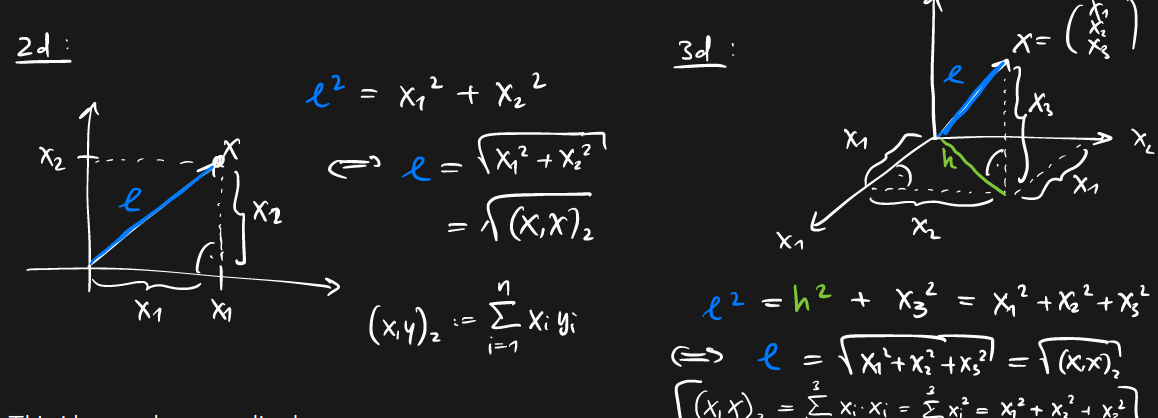
\includegraphics[width=1\textwidth]{media/pythagoras}
~\\}

This idea can be generalized to: \vspace{-0.25cm}
\begin{defi}[Euclidean Norm] 
	The Euclidean norm of a vector $x\in \F^n$ is defined by $$\|x\|_2 := \sqrt{\sum_{i=1}^n |x_i|^2}= \sqrt{x^H x} $$
	where $|a+ib|^2 := a^2+b^2$ denotes the absolute value of a complex number.
	For a real vector $x\in \R^n$ this simplifies to
	$\|x\|_2 := \sqrt{\sum_{i=1}^n x_i^2}= \sqrt{x^\top x}. $
\end{defi}
\small
{ $\rightarrow$ We will also get to know other ``norms'' (e.g., Manhattan norm or maximum norm).}\\


\end{frame}
\begin{frame} 
	\textbf{Relating the inner product to \text{projections}}~\\\vspace{0.2cm}
	Let us consider $\F=\R$. As a special case of the so-called \textbf{Cauchy Schwarz inequality} one can show that, for any two real vectors $x,y\in \R^n$, 
	\begin{equation*}\label{eq:cauchyschwarz_l2} \color{satzrot}
	\left|x^Ty\right|\le \|x\|_2\cdot\|y\|_2.
	\end{equation*}
	~\\
	This is equivalent to (assumed both vectors are nonzero, otherwise trivial case)
	\begin{equation*}
	-1 \leq \frac{x^Ty}{\|x\|_2\cdot\|y\|_2} = \left(\frac{x }{\|x\|_2 }\right)^T \left(\frac{y}{\|y\|_2}\right) \leq 1.
	\end{equation*}
	~\\~\\
	Since $\cos\colon (0, \pi) \to (-1,1)$ is bijective, we find an uniquely defined angle $\alpha \in (0, \pi)$, so that
	$$\cos(\alpha) = \frac{x^Ty}{\|x\|_2\cdot\|y\|_2} ~~~\left(\in (-1,1)\right). $$
	\begin{center}
		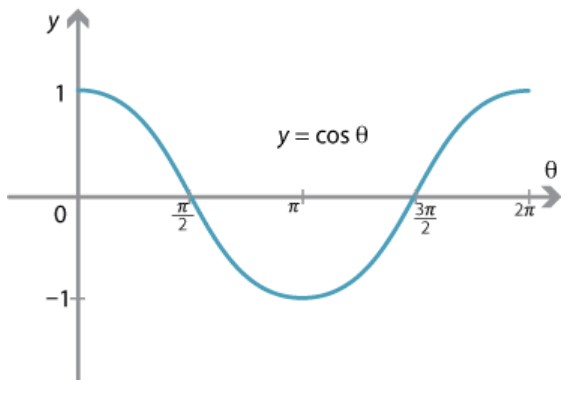
\includegraphics[width = 0.3\textwidth]{media/cosine}
	\end{center}
{\color{defgruen}We also use the notation $\alpha:=\sphericalangle(x,y)$}, since $\alpha$ can be considered´ the angle between $x$ and $y$.	
\end{frame}

\begin{frame}
	
		Geometric insights from the identity 
		$$\text{cosine} = \frac{\text{adjacent}}{\text{hypotenuse}} .$$
\Hide{~\\
		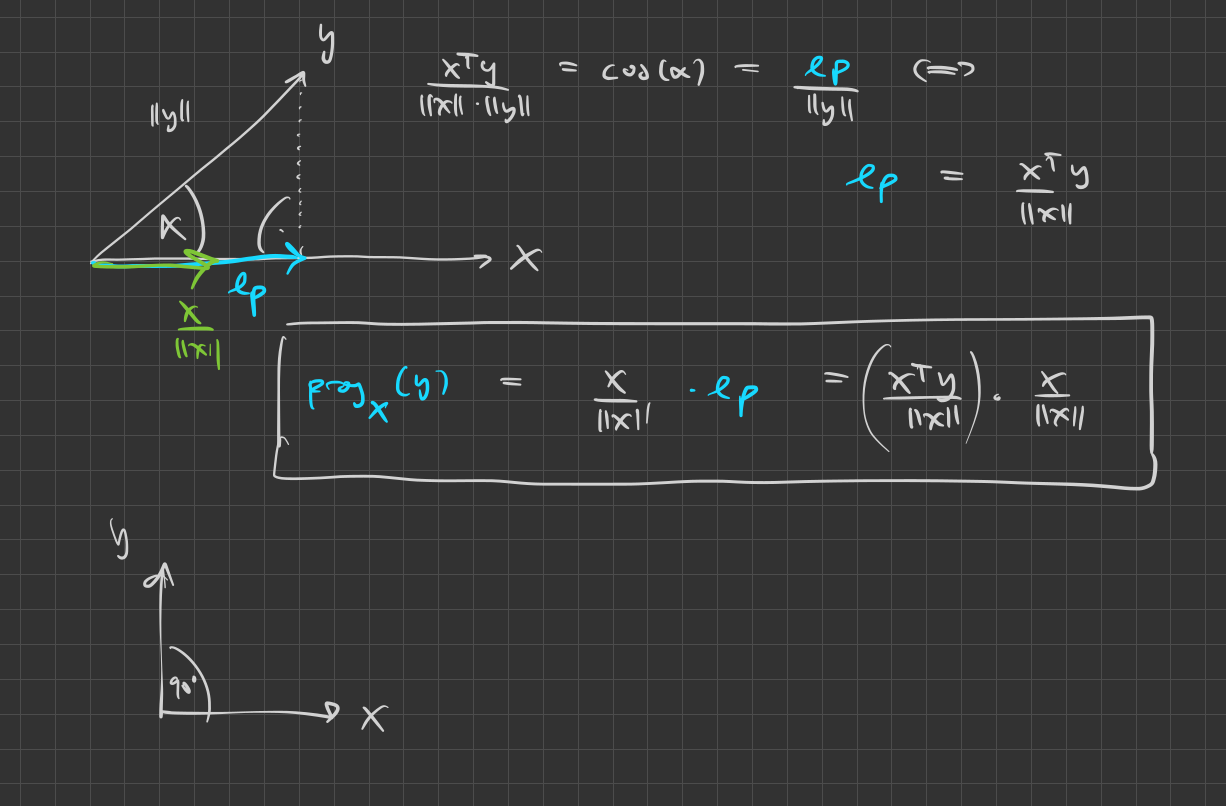
\includegraphics[width=0.95\linewidth]{media/projections}
}
\end{frame}



%%%%%%%%%%%%%%%%%%%%%%%%%%%%%%%%%%%%%%%%%%%%%%%%%%%%%%%%%%%%%%%%%%%%5
% GENERAL NORMS AND INNER PRODUCTS
%%%%%%%%%%%%%%%%%%%%%%%%%%%%%%%%%%%%%%%%%%%%%%%%%%%%%%%%%%%%%%%%%%%%%

%\elomath{
%\begin{frame}
%	\Hide{
%		~\\
%		normalization, unit circle: 3 pictures (simple, rotated, general+projection)\\
%		-- (1) $x$ = unit vector\\ 
%		(2) you can always rotate $x$ to the unit vector (this rotation depends on $x$ and has to be applied to $y$, so that $y_1$ changes to a $\tilde{y}_1(x) = x^Ty$):\\~\\
%		-- relation to projections,
%		$$\frac{x^Ty}{\|x\|_2\cdot\|y\|_2} = \cos(\alpha) = \frac{\ell}{\|y\|_2} ~~\Leftrightarrow~~ \ell = \frac{x^Ty}{\|x\|_2} $$
%		We define: $$\text{proj}_x(y) := \frac{x^Ty}{\|x\|_2} \frac{x}{\|x\|_2} $$ 
%		~\\
%		-- allude to orthogonality
%	}
%\end{frame}
%\begin{frame} 
%\pictures{
%	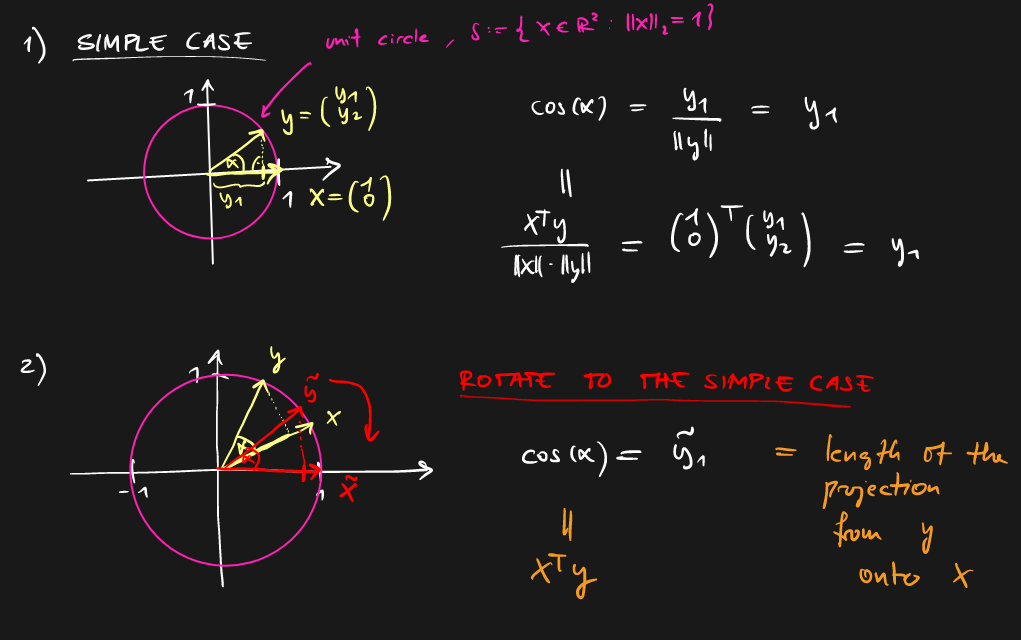
\includegraphics[width=0.7\textwidth]{media/innerproduct-as-projection1}\\
%	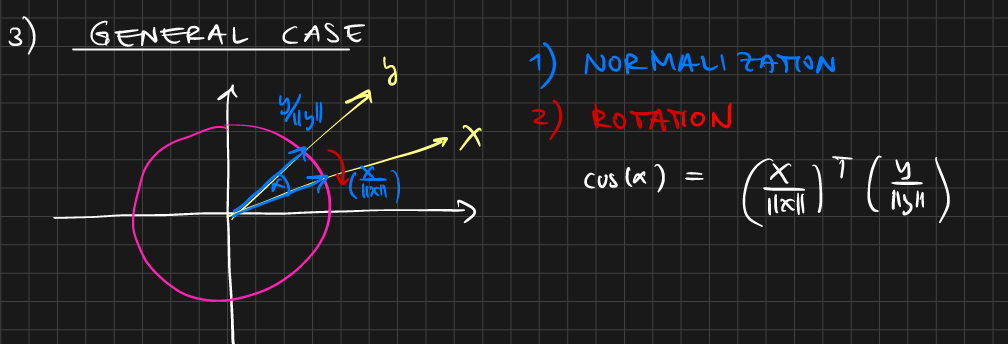
\includegraphics[width=0.7\textwidth]{media/innerproduct-as-projection2}
%}
%\end{frame}
%}



%\only<article>{
%	{\large \textbf{Question:} Do all ($p$-)norms correspond to an inner product?}
%	\begin{lemma}[Polarization identity]\label{lem:polarization}
%		Let $(\cdot,\cdot)\colon \R^n\times \R^n \to \R$ be an inner product on $\R^n$ and $\|\cdot\|\colon \R^n \to [0,\infty)$, $\|v\| := \sqrt{(v,v)}$. Then
%		\[
%		(v,w)=\frac14\left(\|v+w\|^2-\|v-w\|^2\right).
%		\]
%	\end{lemma}
%	%
%	%
%	\begin{re}
%		By Corollary \ref{cor:innerproduct_defines_norm} each inner product induces a norm. However, with the help of Lemma \ref{lem:polarization} one can show that, e.g., the norms $\|\cdot\|_1$ or $\|\cdot\|_\infty$ are not induced by an inner product, i.e., there is no mapping $(\cdot,\cdot)$ satisfying Definition \ref{def:innerproduct} so that $\|v\|_1 = \sqrt{(v,v)}$.
%	\end{re}
%	interpretation in terms of angle
%
%\begin{frame}
%\Subsection{Scalar product and Norm}
%%
%\begin{itemize}
%	\item \textbf{Question:} Can we ``solve'' a linear system, where the matrix is not invertible or even not quadratic? -- in which sense? \\
%	$\rightarrow$ this is the topic of the following two sections.
%	\item \textbf{Recall:}\\
%	$Ax=b$ solvable ~~$\Leftrightarrow$~~ $A\in GL_n(\F )$, which means $x=A^{-1}b$~~ $\Rightarrow$~~ $Ax-b=0$ 
%	\item 
%	\textbf{Idea:} What about making $Ax-b\in\F^n$ just very small, if $A$ is any matrix?
%	\item {\bf What is a small vector?}\\ 
%	We need a length mapping $L:\F^n\to [0,\infty)$ with some plausible properties:
%	\ite
%	\item[(i)] $L(v)=0\ \Rightarrow v=0$ ~~\textit{(positive definite/ point separating)}
%	\item[(ii)] $L(r\cdot v)=|r|\cdot L(v)\, ,\ \forall v\in\F^n, r\in\R$~~\textit{(absolutely homogeneous)}
%	\item[(iii)] $L(v+w)\le L(v)+L(w), \ \forall v,w\in\F^n$ \textit{(subadditive/ triangle inequality)}
%	\eti
%\end{itemize}
%
%\begin{defi}[Norm] \label{def:norm} If a mapping $L\colon\F^n\to[0,\infty)$ satisfies properties (i)-(iii), then it is called a \textbf{norm} and we use the notation
%	$\|v\|:=L(v)$ for $v\in \F^n$. 
%\end{defi}
%\begin{itemize}
%	\item[$\rightarrow$] There are a lot of norms available. For the moment, we focus on the most often used norm and also only on vectors from $\R^n$.
%\end{itemize}
%\Hide{ Example in $\R$: Absolute value $|x|$ for $x\in \R$.}
% 
%\end{frame}
%
%\begin{frame} 
%The standard norm for $x \in \R^n$ is introduced in the following definition.
%\begin{defi}[$p$-norm] \label{def:pnorm}
%	Let $x\in \R^n$ and $p \in [1,\infty]$. Then the $p$-norm $\|\cdot\|_p\colon \R^n \to [0,\infty)$ is defined by
%	\begin{align}
%	\norm{x}_{p} = \left(\sum_{i=1}^n \abs{x_{i}}^p\right)^\frac{1}{p}. \label{def:pnorm}
%	\end{align}	 
%\end{defi}
%\vspace{-0.45cm}
%\begin{ex}
%	\blank
%	\begin{align*}
%	\underline{p=1}: ~~~~&~\norm{x}_{1} = \sum\limits_{i=1}^n \abs{x_{i}} &\text{Manhattan norm}\\
%	\underline{p=2}:~~~~~ &~\norm{x}_{2} = \sqrt{\sum\limits_{i=1}^n x_{i}^2} &\text{Euclidean norm}\\
%	\underline{p=\infty}: ~~~~~&~\norm{x}_{\infty} := \lim\limits_{p \rightarrow \infty} {\norm{x}_{p}} = \max_{i \in \set{1,..,n}}{\abs{x_{i}}} &\text{Maximum norm}
%	\end{align*}
%\end{ex}
%{
%	\blank
%	Proof for identity with $p=\infty$\\
%	w.l.o.g. we assume that $\abs{x_{1}}$ is maximal. There are may b $k$ further entries with $\abs{x_{i}} = \abs{x_{1}}$ then \\
%	$\norm{x}_{p} = \left(\sum\limits_{i=1}^n {\left|x_{i}\right|}^p\right)^\frac{1}{p} = \abs{x_{1}} \left(k + \underbrace{{\left|\frac{x_{k+1}}{x_{1}}\right|}^p}_{\rightarrow 0} + \cdots +\underbrace{{\left|\frac{x_{n}}{x_{1}}\right|}^p}_{\rightarrow 0}\right)^\frac{1}{p} \longrightarrow \abs{x_{1}}$
%	
%	for any $k\in \mathbb{N}$ we have $\sqrt[p]{k} \rightarrow 1, p \rightarrow \infty$ 
%}
%\end{frame}
%
%
%%
%\begin{lemma}
%	The $p$-norm $\|\cdot\|_p$ from \eqref{def:pnorm} is indeed a norm as introduced in Definition \ref{def:norm}.
%\end{lemma}
%\begin{proof}
%	\blank
%	We exemplary proof this statement for $p\in \{1,2,\infty\}$ (for general proof conduct any linear algebra book). For this purpose we need to verify the three requirements that a norm shall satisfy.	\\ 
%	\textbf{For $1$-norm}\\
%	\begin{align*}
%	\text{Assume w.o.l.g.}\; &v_1 \neq 0 \Rightarrow \abs{v_1}>0 \Rightarrow \sum\limits_{i=1}^n \underbrace{\abs{v_i}}_{\ge 0} \geq \abs{v_1} > 0\\
%	0 = \norm{v}_{1} = &\sum\limits_{i=1}^n \underbrace{\abs{v_{i}}}_{\geq 0} \Rightarrow v_{i} = 0, \forall{i} \Rightarrow v=0\\
%	\norm{r\cdot v}_{1} = &\sum\limits_{i=1}^n \abs{r \cdot v_{i}} = \sum\limits_{i=1}^n \abs{r} \cdot \abs{v_{i}} = \abs{r}\sum\limits_{i=1}^n \abs{v_{i}} = \abs{r}\cdot \norm{v}_{1}\\
%	\norm{v+w}_{1} = &\sum\limits_{i=1}^n \abs{v_{i}+w_{i}} \leq \sum\limits_{i=1}^n (\abs{v_{i}} + \abs{w_{i}}) = \sum\limits_{i=1}^n \abs{v_{i}} + \sum\limits_{i=1}^n \abs{w_{i}} = \norm{v}_{1} + \norm{w}_{1}
%	\end{align*}
%	\textbf{For $\infty$-Norm}: analogous arguments as for the 1-norm.\\
%	\textbf{For $2$-norm}\\
%	later
%	\begin{align*}
%	0 = \norm{v}_{2} = &\sqrt{\sum\limits_{i=1}^n v_{i}^2} \Rightarrow 0 = \sum\limits_{i=1}^n v_{i}^2 \Rightarrow v_{i}^2 = 0, \forall{i} \Rightarrow v_{i}=0, \forall{i} \Rightarrow v = 0\\
%	\norm{r\cdot v}_{2} = &\sqrt{\sum\limits_{i=1}^n (r \cdot v_{i})^2} = \sqrt{\sum\limits_{i=1}^n  r^2 \cdot v_{i}^2} = \sqrt{r^2\sum\limits_{i=1}^n \cdot v_{i}^2} = \abs{r}\sqrt{\sum\limits_{i=1}^n v_{i}^2} = \abs{r}\norm{v}_{2}\\
%	\norm{v+w}_{2} &\leq \norm{v}_{2} + \norm{w}_{2}
%	\end{align*}
%	triangle inequality more difficult (later)\\~\\
%\end{proof}
% 
%\begin{frame} 
%%
%\begin{defi}[Inner product]\label{def:innerproduct}
%	A mapping $(\cdot,\cdot)\colon \R^n\times \R^n \to \R$ is called \textbf{inner product} (or \textbf{scalar product}) on $\R^n$ if it satisfies
%	\begin{itemize}
%		\item[(i)] $\forall v,w \in \R^n: ~(v,w) = (w,v)$~~~~~~~~~~~~~~~~~~~~~~~~~~~~~~~~~~~~~~~~~~(symmetric)
%		\item[(ii)]$\forall v,w_1,w_2 \in \R^n: ~(v,w_1+w_2) = (v,w_1)+(v,w_2)$
%		\item[] $\forall v,w \in \R^n, r \in \R: ~ (v,r\cdot w)=r\cdot(v,w)$~~~~~~~~~~~~~~~~~~~~~~~~~~~~~~(linear in its second argument)
%		\item[(iii)] $\forall v \in \R^n\backslash\{0\}: ~ (v,v) > 0$ ~~~~~~~~~~~~~~~~~~~~~~~~~~~~~~~~~~~~~~~~~~~~~(positive definite)
%	\end{itemize}
%	%
%\end{defi}
%~\\
%{\large \textbf{Question:} Relation between norms and inner products?}
%\begin{theo}[Cauchy-Schwarz inequality]\label{theo:cauchyschwarz}
%	Let $(\cdot,\cdot)\colon \R^n\times \R^n \to \R$ be an inner product on $\R^n$ and $\|\cdot\|\colon \R^n \to [0,\infty)$, $\|v\| := \sqrt{(v,v)}$. Then there holds the \textbf{Cauchy-Schwarz inequality}: 
%	$$\left|(v,w)\right|\le \|v\|\cdot\|w\|.$$
%\end{theo}
%\begin{proof}
%	\blank
%	Property (3) is shown via Cauchy-Schwarz inequality, which is trivially correct, if $v=0$ or $w=0$. Now, we assume that both are nonzero. Obviously, $z^\top z\ge 0$, for any $z\in\R^n$. We choose $z:=v/\|v\|_2-w/\|w\|_2$ and achieve
%	\[
%	0\le z^\top z=\frac{v^\top v}{\|v\|_2^2}-2\frac{v^\top w}{\|v\|_2\cdot\|w\|_2}+\frac{w^\top w}{\|w\|_2^2}=2-2\frac{v^\top w}{\|v\|_2\cdot\|w\|_2}
%	\Rightarrow \left|v^\top w\right|\le \|v\|_2\cdot\|w\|_2
%	\]
%\end{proof}
%\end{frame}
%
%
%\begin{frame} 
%\textbf{We find:} Each inner product defines a norm.
%\begin{corollary} \label{cor:innerproduct_defines_norm}
%	Let $(\cdot,\cdot)\colon \R^n\times \R^n \to \R$ be an inner product on $\R^n$, then $\|\cdot\|\colon \R^n \to \R$,
%	$$\|v\| := \sqrt{(v,v)}$$ 
%	defines a norm on $\R^n$.
%\end{corollary}
%\begin{proof}
%	\blank
%	Properties (1) and (2) are obvious. 
%	C-S leads to $\|v+w\|_2^2=(v+w)^\top(v+w) = v^Tv +  2v^Tw+w^Tw\le v^Tv +  2\norm{v}_2\norm{w}_2+ w^Tw\le(\|v\|_2+\|w\|_2)^2$, which is the triangle inequality.
%\end{proof}
%%
%\end{frame}
%%
%}
%
%
%
%
%\only<article>{
%\begin{frame} 
%{\large \textbf{Question:} Can we characterize \emph{all} inner products on $\R^n$?}
%\begin{defi}[Symmetric and positive definite matrices]
%	Let $A \in \R^{n\times n}$. 
%	\begin{itemize}
%		\item[(i)] $A$ is called \textbf{symmetric}, if $A = A^T$.
%		\item[(ii)] $A$ is called \textbf{positive definite}, if $v^\top Av>0\, ,\ \forall v\in\R^n\setminus\{0\}$.
%	\end{itemize}
%	We define the set of all symmetric and positive definite matrices by $$\R^{n\times n}_{spd} := \{ A \in \R^{n\times n}\colon A~ \text{sym and pos. def.}\}\subset GL_n(\R) \subset \R^{n\times n}.$$
%\end{defi}
%\begin{theo}[Characterization]\label{theo:characterization_inner_products}
%	Let $(\cdot,\cdot)\colon \R^n\times \R^n \to \R$ be a mapping on $\R^n$. Then:
%	$$ (\cdot,\cdot) ~~\text{inner product}~~ \Leftrightarrow ~~\exists A \in \R^{n\times n}_{spd}\colon (v,w) = (v,w)_A := v^TAw ~~\forall v,w\in \R^n. $$
%	%A symmetric and positive definite matrix $A\in\R^{n\times n}$ defines a scalar product $(v,w)_A:=v^\top Aw$. On the other hand, any scalar product $(v,w)$ can be written as $(v,w)=v^\top Aw$ with an appropriate symmetric and positive definite matrix $A$.
%\end{theo}
%\end{frame}
%
%\begin{frame}
%\begin{proof} 
%	\blank	
%	``$\Leftarrow$'' obvious. ``$\Rightarrow$'' is shown by the construction:
%	\[
%	A=[a_{ij}]_{ij}\, , \qquad a_{ij}:=(e_i,e_j)\text{, where } e_i:=
%	\bbmat \delta_{1,i}, \ldots , \delta_{n,i}\ebmat^\top
%	\]
%	\begin{itemize}
%		\item[a)] let A be symmetric and positive definite: i.e. $A^T = A$ and $v^T Av > 0, \forall{v \neq 0}$
%		\begin{enumerate}
%			\item[(i)] $(v,w)_A = v^T Aw = (v^T Aw)^T = w^T A^T v = w^T Av = (w,v)_A$
%			\item[(ii),(iii)] $(v, \alpha w_1 + \beta w_2)_A = v^T A(\alpha w_1 + \beta w_2) = v^T A(\alpha w_1) + v^T A(\beta w_2) = \alpha v^T Aw_1 + \beta v^T Aw_2 = \alpha(v,w_1)_A + \beta(v,w_2)_A$
%			\item[(iv)] $(v,v)_A^{\frac{1}{2}} = (v^T Av)^{\frac{1}{2}}$
%		\end{enumerate}
%		\begin{align*}
%		\text{norm(1):}\;\; &0 = (v,v)_A^{\frac{1}{2}} = (v^T Av)^{\frac{1}{2}} \Rightarrow v=0,\; \text{because A is p. d.}\\
%		\text{norm(2):}\;\; &(r\cdot v, r\cdot v)_A^{\frac{1}{2}} = [(r\cdot v)^T A(r\cdot v)]^{\frac{1}{2}} = [r^2 v^T Av]^{\frac{1}{2}} = \mid r \mid (v,v)_A^{\frac{1}{2}}\\
%		\text{norm(3):}\;\; &\text{triangle inequality: can be shown for}\; (.,.)_A^{\frac{1}{2}}\; \text{as for} \;\norm{}_2\; \\&\text{by generalizing Cauchy-Schwartz (T.4.4) to} (.,.)_A\\
%		\end{align*}
%		\item[b)] any $v \in \mathbb{R^n}$ is given as $v  = \sum\limits_{i=1}^n v_i e_i$ , similar: $w = \sum\limits_{i=1}^n w_i e_i$\\[5pt]
%		$\begin{pmatrix}
%		        v_{1} \\
%		        v_{2} \\
%		        \vdots \\
%		        v_n 
%		    \end{pmatrix} = v_1 \begin{pmatrix}
%		        1 \\
%		        0 \\
%		        0 \\
%		        \vdots \\
%		        0 
%		    \end{pmatrix} + v_2  \begin{pmatrix}
%		        0 \\
%		        1 \\
%		        0 \\
%		        \vdots \\
%		        0 
%		    \end{pmatrix} + \cdots + v_n  \begin{pmatrix}
%		        0 \\
%		        0 \\
%		        0 \\
%		        \vdots \\
%		        1 
%		    \end{pmatrix}  $
%		$\Rightarrow (v,w) = (\sum\limits_{i=1}^n v_i e_i, \sum\limits_{j=1}^n w_j e_j)$\\[5pt]
%		$=\sum\limits_{i=1}^n v_i \sum\limits_{j=1}^n w_j (e_i,e_j)$\\[5pt]
%		$=\sum\limits_{i=1}^n \sum\limits_{j=1}^n v_i\underbrace{(e_i, e_j)}_{A:=[(e_i,e_j)]_{ij}} w_j = v^T Aw$\\[5pt]
%		This matrix is obviously s. p. d.
%	\end{itemize}
%\end{proof}
%\end{frame}
%}


% ORTHOGONAL MATRIX
\begin{frame}
\Subsection{Orthogonal Vectors and Matrices}
Let us again consider the relation 
$$\cos(\alpha) = \frac{x^Ty}{\|x\|_2\cdot\|y\|_2},~~~x,y\in\Rn  .$$
Now let us assume that the angle $\alpha = \sphericalangle(x,y)$ between the two vectors $x,y$ is $90^\circ$, i.e., $\alpha =\pm \frac{\pi}{2}$, meaning that they are \textit{perpendicular}. Then we find
\begin{equation*}
 ~~~0 = \cos\left(\pm \frac{\pi}{2}\right) = \frac{x^Ty}{\|x\|_2\cdot\|y\|_2}  
 ~~~~~~\Leftrightarrow~~~~~~ 0 = x^\top y.
\end{equation*}
~\\~\\
In mathematics we call this \textit{orthogonal} and make it a general definition:\vspace{-0.25cm}
\begin{defi}[Orthogonal/-normal vectors]~\\
\begin{itemize}
	\item[i)] Two vectors $x,y \in \F^n$ are called \textbf{orthogonal} if $(x,y)_2 = x^H y  = 0$.
	\item[ii)] Two vectors $x,y \in \F^n$ are called \textbf{orthonormal} if they are orthogonal and have length $1$ (i.e., $\|x\|_2=\|y\|_2=1$).
	\item[iii)] Vectors $x_1, \ldots, x_r \in \F^n$ are called (mutually) \textbf{orthogonal (orthonormal)} if $x_i, x_j$ are \textbf{orthogonal (orthonormal)} for all possible pairs $i\neq j \in \{ 1,\ldots, r\}$.
\end{itemize} 
\end{defi} 
~\\
{\color{satzrot} One can show that:
\begin{equation}\label{eq:orthoImpliesIndepen}
x,y ~~\text{orthogonal} ~~~\Rightarrow ~~~ x,y~~\text{linearly independent} .
\end{equation}
}
\Hide{~\\
%\textbf{Example: Identity matrix; rotate the unit vectors; rotation matrix; reflection?}\\
\small Counter example for backwards implication: $x=\begin{pmatrix}1\\0\end{pmatrix},y=\begin{pmatrix}1\\1\end{pmatrix}$}
\end{frame}

\begin{frame}
	\Hide{
\begin{example} \label{ex:orthogonalVecs}
	~\\
	For $\F=\R$ and $n=2$ consider, e.g.,
	 \begin{itemize}
	 	\item Standard basis vectors.
	 	\item Rotation of the standard basis vectors.
	 \end{itemize}
\end{example}	

}
\end{frame}

\begin{frame}
\textbf{Now let us extend this notion to matrices:}~\\~\\
For this purpose observe that the matrix-matrix product $Q^HQ$ for $Q \in \F^{n \times n}$ contains all possible inner products of its columns:\\
\Hide{
	~\\
{\centering
$
\underbrace{\begin{pmatrix}
	-&\overline{q_1}^\top&-\\
	-&\overline{q_2}^\top&-\\
	&\vdots& \\
	-&\overline{q_n}^\top&-
	\end{pmatrix}}_{Q^H}
\underbrace{\begin{pmatrix}
	|&|& &|\\
	q_1&q_2&\cdots&q_n\\
	|&|& &|
	\end{pmatrix}}_{Q}
=\begin{pmatrix}
q_1^Hq_1&\cdots&q_1^Hq_n\\
q_2^Hq_1&\cdots&q_2^Hq_n\\
\vdots&\ddots&\vdots\\
q_n^Hq_1&\cdots&q_n^Hq_n
\end{pmatrix}
~~~~~\left(=\begin{pmatrix}
1&0&\cdots&0\\
0&1&\ddots&\vdots\\
\vdots&\ddots&\ddots&0\\
0&\cdots&0&1
\end{pmatrix}\right)
$
~\\
}
}
%~\\\vspace{3cm}
~\\Let us assume that the columns of $Q$ are mutually ortho\textit{normal}, then $$Q^HQ = I_n .$$
Since this is a central property, we make this a definition:\vspace{-0.25cm}
\begin{defi}[Orthogonal/Unitary matrix]
	A matrix $Q\in\F^{n\times n}$ is called \textbf{\emph{unitary}}, if $$Q^HQ =I_n.$$\\
	For a real matrix $Q\in\R^{n\times n}$ this condition simplifies to $Q^TQ =I_n$, in which case we then call the matrix \textbf{\emph{orthogonal}}.
\end{defi}
\Hide{
Since orthogonality implies linear independence (see statement \eqref{eq:orthoImpliesIndepen}) we know that \textbf{orthogonal matrices are invertible}. From the defining equation $Q^T Q=I_n$ we can even deduce its inverse
 $$  Q^{-1} = Q^T$$ and therefore also $QQ^T=I_n$.\\
 \vspace*{0.2cm}
 $\rightarrow$ This is one (of the many) reasons why the property of orthogonality is very desirable.
}
\end{frame}


\begin{frame}
	\textbf{Understanding $QQ^\top(\cdot)$ as orthogonal projection}~\\~\\
	\Hide{
	For a vector $q \in \Rn$ of length $1$, i.e., $\|q\|_2=1$, and a vector $y\in\Rn$ we find
	$$\text{proj}_q(y) =  (q^\top y) \cdot q.$$
	Now let $Q = [q_1,\ldots, q_n]\in\Rnn$ be an orthogonal matrix (i.e., columns $q_i$ are mutually orthonormal), then
	$$y = I \cdot y 
	=  QQ^\top y 
	= Q \begin{pmatrix}
	q_1^\top y \\ \vdots \\ q_n^\top y
	\end{pmatrix}
	= \sum_{i=1}^n q_i^\top y \cdot q_i
	= \sum_{i=1}^n \text{proj}_{q_i}(y).$$
	With other words, in order to obtain the coordinates of $y$ with respect to the \textit{orthonormal} basis $\{q_1,\ldots, q_n\}$ we solely have to project $y$ onto each basis vector $q_i$.
	\Vspace{1cm}
	\textbf{Example}\\
	Famous related examples from signal processing include the Discrete Cosine Transform (DCT) and the Discrete Fourier Transform (DFT) which can be written as a matrix--vector product $Q^\top(\cdot)$ with an orthogonal/unitary matrix $Q$. In this context, the $q_i$ may correspond to discrete periodic functions of different frequency. For a time-discrete signal 
	$$y=(y_1,\ldots, y_n)^\top \in \Rn$$ 
	one says that the transformed signal 
	$$Q^\top y = (q_1^\top y,\ldots,q_n^\top y)^\top$$ 
	lives in the frequency space.
	
%TODO
%keep?
%	\textbf{Characterization of orthogonal matrices:}\\[0.2cm]
%\textit{Orthogonal matrices are matrices which do not change angle or length, i.e., }
% \begin{itemize}
% 	\item \textit{isometric}: $\|Qx\|_2 = \|x\|_2$
% 	\item \textit{isogonic}: $(Qx, Qy)_2 = (x,y)_2$
% \end{itemize}
%\vspace{0.3cm}
%More precisely, \textit{Reflections} and \textit{rotations} (and combinations).
}
\end{frame}

\begin{frame}[c]
	\centering
	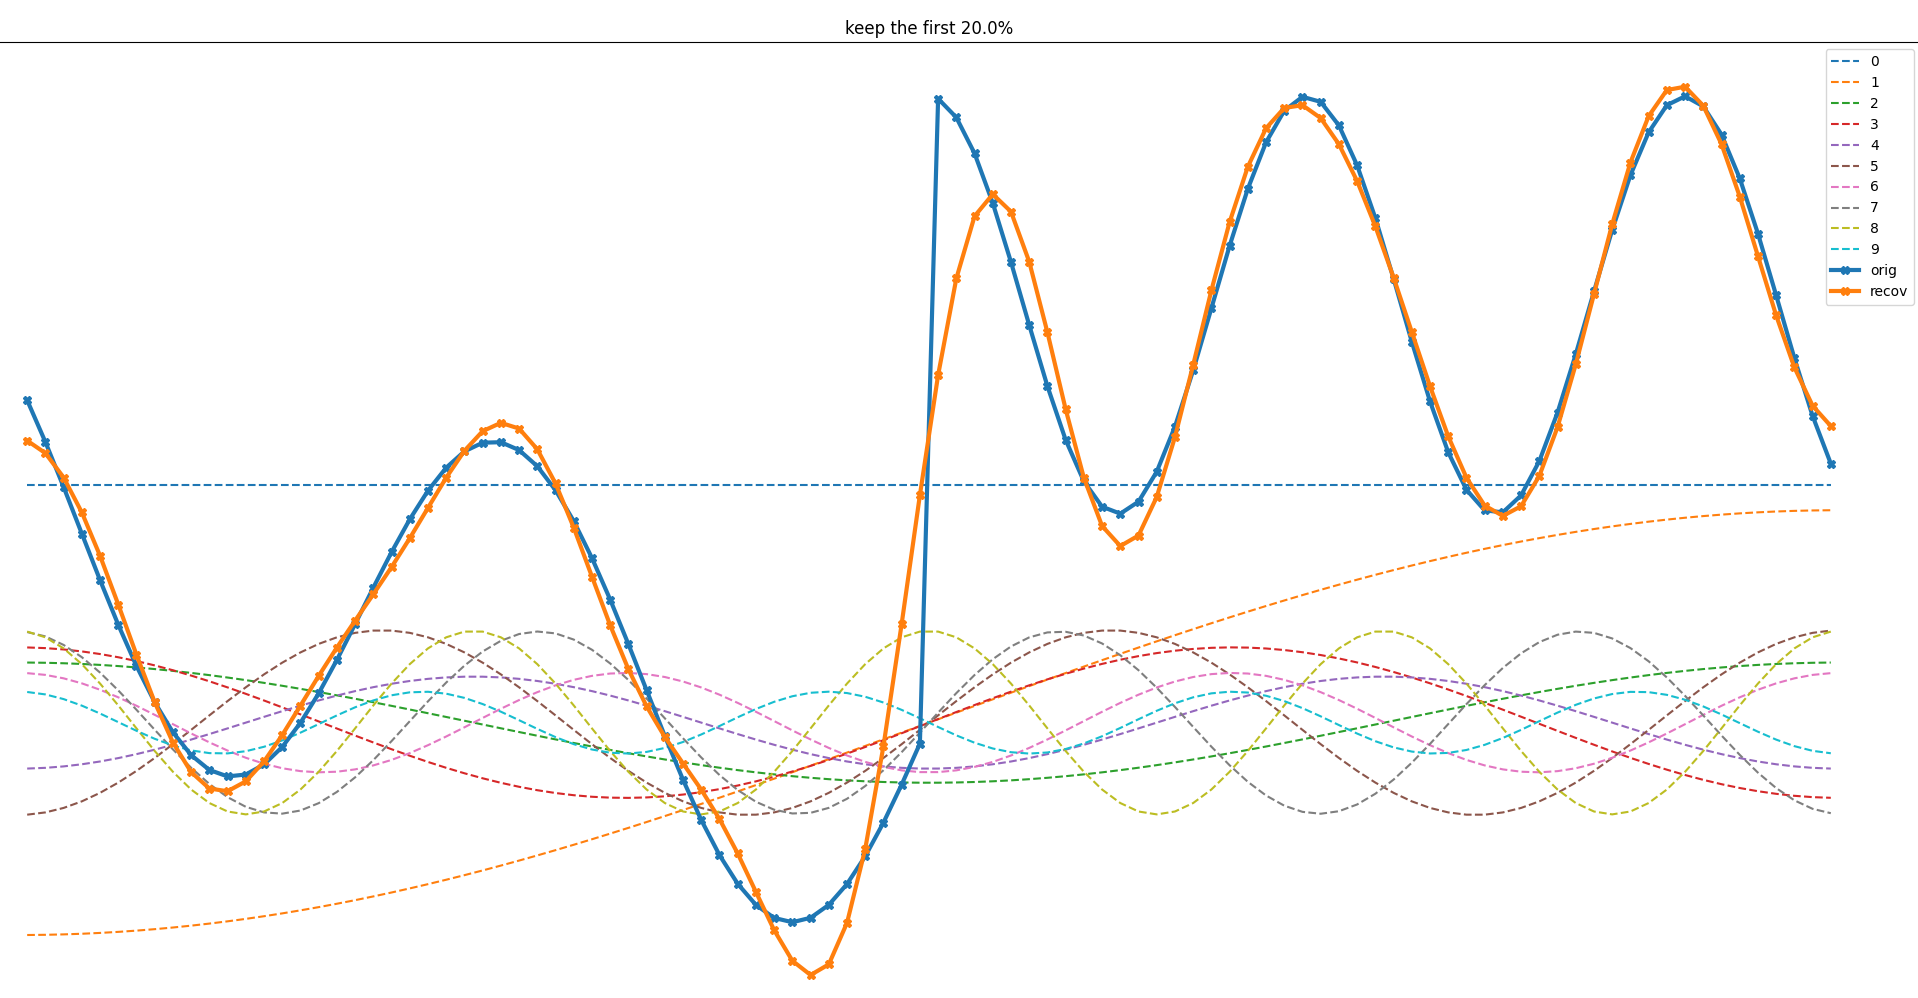
\includegraphics[width=0.99\textwidth]{./media/dct-1d.png}
	1-d DCT compression example (where high frequencies are removed):
	$$
	y 
	= \sum_{i=1}^n q_i^\top y \cdot q_i
	\approx \sum_{i=1}^m q_i^\top y \cdot q_i ~~~(m<n).$$
\end{frame}
\begin{frame}[c]
	\centering
	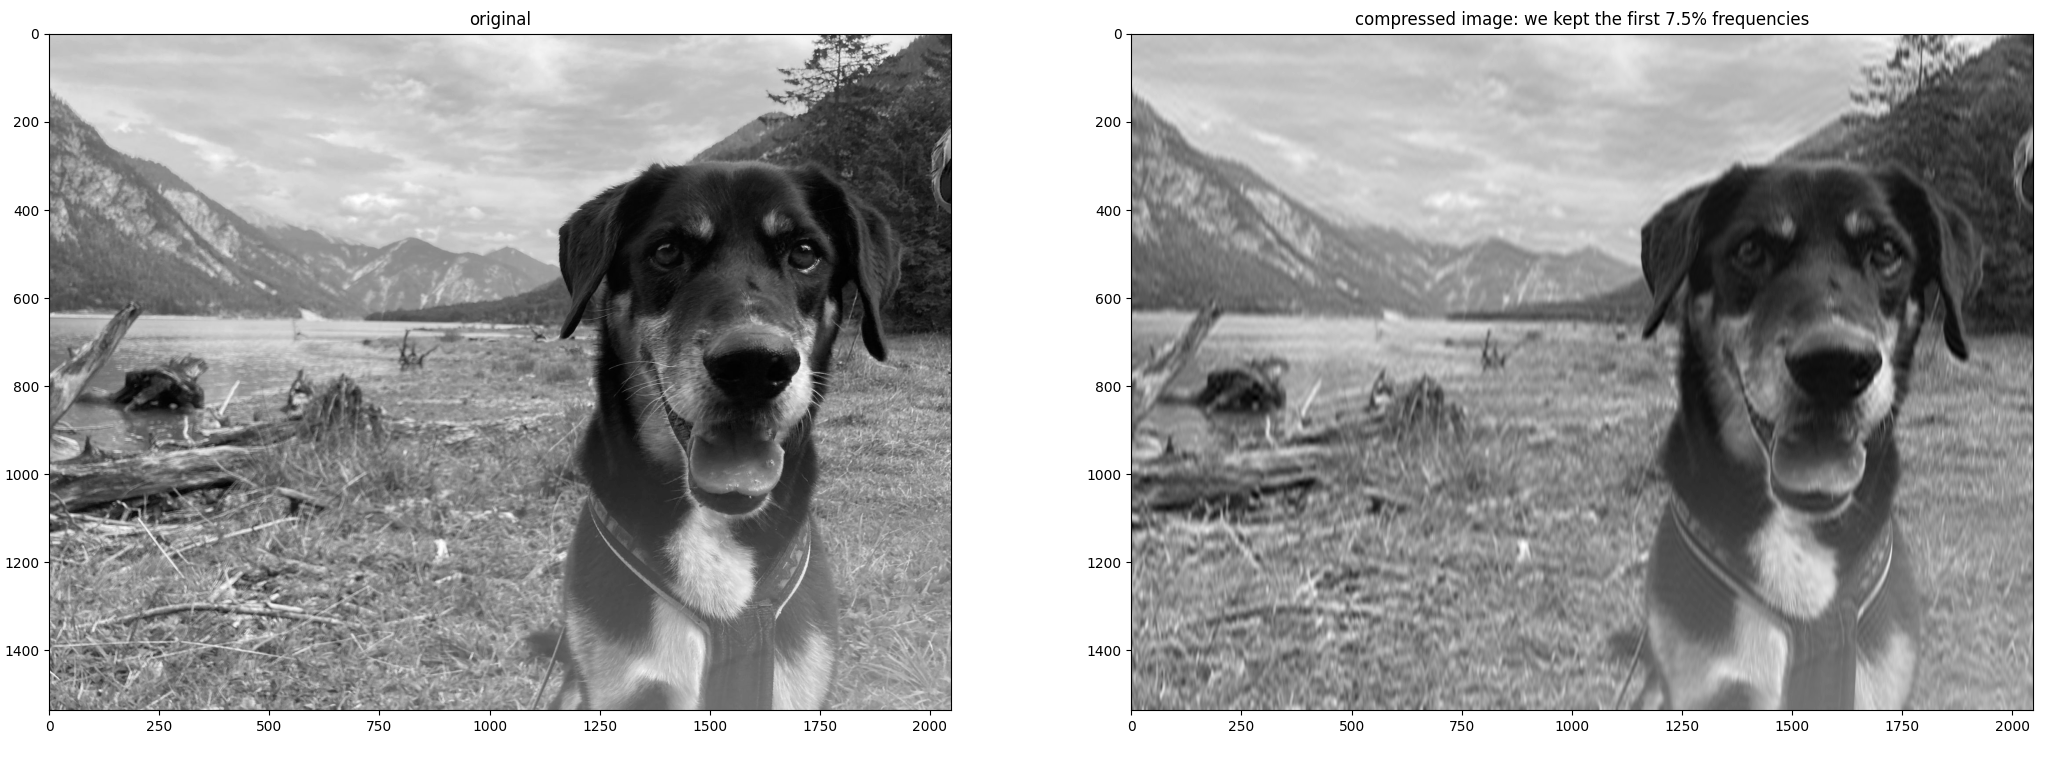
\includegraphics[width=0.99\textwidth]{./media/dct-2d.png}
	2-d DCT compression example (where high frequencies are removed)
\end{frame}


 \begin{frame}
 \Subsection{The Determinant}
  \textbf{Aim:} 
  For $n$ vectors in $\F^n$ we want to have a \textit{measure of linear independence}\\[0.1cm]
  -- or equivalently a \textit{volume measure} for the parallelotope spanned by these vectors  ~\\[0.1cm]
  -- or equivalently a \textit{measure for the invertibility} of a matrix in $\F^{n\times n}$~\\
  	\Hide{~\\
  		\small	Why are all these measures the same?\\
  		\begin{itemize}
  			\item $n$ linear dependent vectors do not span a volume in $\Fn$.
  			\item Linear independent columns of a quadratic matrix imply invertibility.
  		\end{itemize}
  	\pictures{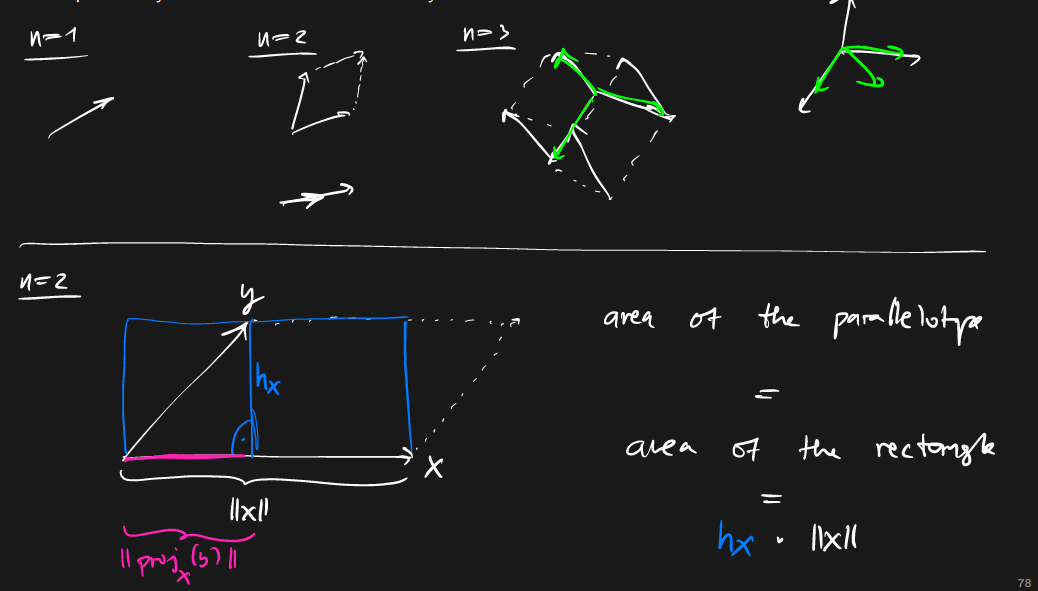
\includegraphics[width=0.8\textwidth]{media/determinant}}}
\end{frame}

%%
\begin{frame}
	\Hide{\small
Let us derive a formula in the two--dimensional case: Let 
	\begin{center}
		$a := $ area of the parallelogram $=$ area of rectangle $= h_x \cdot \|x\|_2$.
	\end{center}
	By the Pythagorean identity we obtain: 
	\begin{align*}
	h_x^2 + \|\text{proj}_x(y)\|_2^2 &= \|y\|_2^2\\
	\Leftrightarrow h_x^2 & =\|y\|_2^2 - \|\text{proj}_x(y)\|_2^2
	=\|y\|_2^2 - \frac{(x^Ty)^2}{\|x\|_2^2}\\
	&= \frac{\|y\|_2^2\|x\|_2^2 - (x^Ty)^2}{\|x\|_2^2} \\
	&= \frac{(y_1^2 + y_2^2)(x_1^2+x_2^2) - (x_1y_1 + x_2y_2)^2}{\|x\|_2^2}\\
	& = \ldots \\
	&=   \frac{(x_1y_2 -x_2y_1)^2}{\|x\|_2^2}.
	\end{align*}
	Thus $$h_x = \left|\frac{x_1y_2 -x_2y_1}{\|x\|_2} \right| = \frac{\left|x_1y_2 -x_2y_1\right|}{\|x\|_2} , $$ which implies $$a = |x_1y_2 -x_2y_1| =: |\det(A)|.$$
}
\end{frame}

% FORMULA FOR THE DETERMINANT
\begin{frame}
In general, there is the following (recursive) formula, which we use as the definition here: \vspace{-0.2cm}
\begin{definition}[Laplace formula]\label{def:Laplace-formula} Let
$A \in \F^{n\times n} $ 
and let
$ A_{ij} \in \F^{(n-1) \times (n-1)} $ be
the matrix resulting from erasing the $i$-th row and $j$-th column. Then the mapping $\det\colon \F^{n\times n} \to \F $ defined by
%
\[
\det(A) = \sum^n_{j=1}(-1)^{i + j} a_{ij} \det(A_{ij})\, ,\quad \text{for a fixed but arbitrary} ~~i \in \left\{1, \ldots, n \right\},
\]
is called the \textbf{determinant} (of $A$), where $\det(a) := a$ for $a\in\R = \R^{1\times 1}$.
\end{definition}
{\color{satzrot} One can show: The determinant is a well-defined function, i.e., by the formula above the function $\det(\cdot)$ assigns to each matrix $A \in \Fnn$ exactly one number in $\F$.}\\
\vspace{0.5cm}
\textbf{Laplace formula for $n=2$ and $n=3$:}\\\vspace{0.2cm}
$\bullet~ n=2$ ~{\small (we fix $i=1$)}  \\ \vspace{0.2cm}
\Hide{Here we have $$ \det(A) =\sum^2_{j=1}(-1)^{1 + j} 
a_{1j} \det (A_{1j})$$ 
{\footnotesize $A_{11} = \begin{pmatrix}
	\textcolor{red}{a_{11}} & \textcolor{red}{a_{12}}\\
	\textcolor{red}{a_{21}} & a_{22}
	\end{pmatrix} = [a_{22}],~~
	A_{12} = \begin{pmatrix}
	\textcolor{red}{a_{11}} & \textcolor{red}{a_{12}}\\
	a_{21} & \textcolor{red}{a_{22}}
	\end{pmatrix} = [a_{21}] $,~~
    $A_{21} = \begin{pmatrix}
	\textcolor{red}{a_{11}} & a_{12}\\
	\textcolor{red}{a_{21}} & \textcolor{red}{a_{22}}
	\end{pmatrix} = [a_{12}], ~~
	A_{22} = \begin{pmatrix}
	a_{11} & \textcolor{red}{a_{12}}\\
	\textcolor{red}{a_{21}} & \textcolor{red}{a_{22}}
	\end{pmatrix} = [a_{11}] $}\\[0.5cm]
So that all in all
$$ \det(A) = (-1)^{1+1} a_{11} \det(A_{11}) + (-1)^{1+2} a_{12} \det(A_{12}) = a_{11} \cdot a_{22} - a_{12}\cdot a_{21}$$ 
% \underline{2nd option:} $\det(A) = (-1)^{2+1} a_{21} \det(A_{21}) + (-1)^{2+2} a_{22} \det(A_{22}) = -a_{21}\cdot a_{12} + a_{22}\cdot a_{11}$
}
~\\
$\bullet~ n=3:$ \textit{Sarrus rule} (exercise)
\only<article>{
	\begin{itemize}
		\item[] $\det(A)=\det\left(\begin{pmatrix}
		\textcolor{cyan}{a_{11}} & \textcolor{orange}{a_{12}} & \textcolor{cyan}{a_{13}}\\
		\textcolor{orange}{a_{21}} & \textcolor{cyan}{a_{22}} & \textcolor{orange}{a_{23}}\\
		\textcolor{cyan}{a_{31}} & \textcolor{orange}{a_{32}} & \textcolor{cyan}{a_{33}}
		\end{pmatrix}\right)$\\
		\item[] $ = a_{11} \cdot det\begin{pmatrix}
		\textcolor{cyan}{a_{22}} & \textcolor{orange}{a_{23}} \\
		\textcolor{orange}{a_{32}} & \textcolor{cyan}{a_{33}}
		\end{pmatrix} - a_{12} \cdot det\begin{pmatrix}
		\textcolor{cyan}{a_{21}} & \textcolor{orange}{a_{23}} \\
		\textcolor{orange}{a_{31}} & \textcolor{cyan}{a_{33}}
		\end{pmatrix} + a_{13} \cdot det\begin{pmatrix}
		\textcolor{cyan}{a_{21}} & \textcolor{orange}{a_{22}} \\
		\textcolor{orange}{a_{31}} & \textcolor{cyan}{a_{32}}
		\end{pmatrix}$\\
		\item[] $ = a_{11}(a_{22}a_{33}-a_{23}a_{32})-a_{12}(a_{21}a_{33}-a_{31}a_{23})+  a_{12}(a_{21}a_{32}-a_{31}a_{22}) =$\\
		\item[] $ = a_{11}a_{22}a_{33}-a_{11}a_{23}a_{32}-a_{12}a_{21}a_{33}+ a_{12}a_{31}a_{23}+a_{13}a_{21}a_{32}-a_{13}a_{31}a_{22}$\\
\end{itemize}}
\end{frame}

\begin{frame}
	\vspace{0.2cm}
	\vspace{0.99cm}
	One can show:\vspace{-0.2cm}
	\begin{theorem}[Determinant properties]\label{theo:det-rules} The determinant satisfies the following computational rules:
		\begin{itemize}		
		\vspace{0.2cm}\item[i)] $\forall  A \in \F^{n \times n}:~~~\det(A)\neq 0\, \Leftrightarrow A\in GL(n,\F ) ~(\Leftrightarrow \text{columns of $A$ are linearly independent})$
		\vspace{0.2cm}\item[ii)] $\forall  A \in \F^{n \times n}:~~~\det(A^\top)=\det(A)$
		\vspace{0.2cm}\item[iii)] if 
		$ A \in \F^{m \times m}, 
		B \in \F^{m \times n}, 
		C \in \F^{n \times n}$ 
		and
		
		\begin{equation*}
		M : \; = 
		\left(
		\begin {array} {c c} 
		A & B \\ 
		0 & C 
		\end {array} 
		\right)
		\in \F^{(m + n) \times (m + n)}
		\end{equation*}
		
		then
		$ \det M = 
		\det A \cdot \det C $
		
		\vspace{0.2cm}\item[iv)] $\forall A,A' \in \F^{n \times n}:~~~\det(A\cdot A')=\det(A)\cdot\det(A')$
	\end{itemize}
	\end{theorem}
	~\\~\\
	\Hide{	The central result for us is i).}
\end{frame}

%
\begin{frame}
	\textbf{Question:} Are there matrices for which the computation of the determinant is easy?\\~\\
 Yes, as in many other situations it turns out that orthogonal and triangular matrices are easy to treat! More precisely, we find:
 ~\\
 \begin{corollary}[Triangular matrices]\label{cor:det-triangular}
 	Let $U \in \F^{n\times n}$ be upper triangular, i.e., 
 	$$ U = \begin{pmatrix}
 	u_{11} & x & \cdots & x \\
 	0& u_{22} & & \vdots \\
 	\vdots & & \ddots & x\\
 	0 & \cdots &0 & u_{nn}
 	\end{pmatrix}.$$ Then	
 	$$\det(U) = u_{11} \cdot u_{22} \cdot \hdots \cdot u_{nn}.$$
 		In particular, we find
 	$$
 	U~\text{is invertible}~~\Leftrightarrow~~\text{det}(U)\neq 0~~\Leftrightarrow~~\forall i:~u_{ii}\neq 0
 	$$
 \end{corollary}
 \begin{proof} Exercise:
 	For the product formula apply Theorem \ref{theo:det-rules} iii) inductively. The second part then easily follows from Theorem \ref{theo:det-rules} i).
 \end{proof}



~\\
 \begin{corollary}[Orthogonal matrices]
 	Let $Q \in \R^{n\times n}$ be an orthogonal matrix, then $|\det(Q)| = 1$.
 \end{corollary}
 \begin{proof}
 	From Cor. \ref{cor:det-triangular} we find $\det(I)=1$. Then result follows from Theorem \ref{theo:det-rules} ii) and iv).
 \end{proof} 
\end{frame}

%\mode<article>{
%\begin{frame}
%
%{\bf Motivation:} Measure of independence? We seek a volume measure for parallelotopes of the form ~\\
%$ \R^2 $ 
%\begin{minipage}{0.4\textwidth}
%	\unitlength1cm 
%	\begin{picture}(6,4) 
%	\put(1,0.2){\includegraphics[scale=0.75]{LocalFolder/LocalMedia/9_det1.eps}} 
%	\end{picture} 
%\end{minipage}
%$ \R^3 $ 
%\begin{minipage}{0.4\textwidth}
%	\unitlength1cm 
%	\begin{picture}(6,4) 
%	\put(-0,-0){\includegraphics[scale=0.75]{LocalFolder/LocalMedia/9_det2.eps}} 
%	\end{picture} 
%\end{minipage}
%~\\
%Thus, this volume measure should satisfy the following properties:
%\begin{itemize} \footnotesize
%	\item[\textbf{(D1)}]
%	The {\bf unit cube} with edge length 1 should have volume {\bf{1}},
%	
%	\[ \det 
%	\left( \left[ 
%	e_1, \ldots, e_n 
%	\right] \right) 
%	= \det (I_n) = 1
%	\]
%	
%	\textit{$\rightarrow~$``$ \det$ is normed''}
%	%
%	%
%	\item[\textbf{(D2)}] 
%	If two edges coincide, then the parallelotope is {\bf flat} and  und has {\bf volume 0}, 
%	
%	$$ \det \left( \left[ v_1, \ldots, v_n \right] \right) = 0, \text{~~if there exist~} i \not = j\text{~~with~~}v_i = v_j$$
%	
%	\textit{$\rightarrow~$``$ \det $ is alternating''}
%	%
%	%
%	\item[\textbf{(D3)}] 
%	The volume is {\bf linear} in {\bf each edge direction}, i.e., 
%	$ \det $ is linear in each column,
%	\begin{align*}
%	\det([ 
%	v_1, \ldots, v_i  
%	& + \lambda \; 
%	v_i', v_{i+1}, \ldots, v_n 
%	] ) \\
%	&=  \det \left( \left[ 
%	v_1 , \ldots, v_i ,\ldots, v_n 
%	\right] \right) 
%	+ \lambda \; \det 
%	\left( \left[
%	v_1, \ldots, v_i^\prime,
%	\ldots, v_n 
%	\right] \right) 
%	\end{align*}
%	
%	\textit{$\rightarrow~$``$ \det $ is a multi linear form''}
%\end{itemize}
%\end{frame}
%
%% DEFINITION AND PROPERTIES
%\begin{frame}
%%Skriptseite 3
%\begin{definition}[Determinant]\label{Definition 10.1}
%Let  $ \F $ be a field and $ n \in  \N $. Then, we call a mapping
%$$
%\triangle:  \F^{n \times n} \rightarrow  \F ,~~~
%A \mapsto \triangle (A)
%$$
%the {\bf determinant}, if it satisfies properties  (D1, D2, D3).
%Thus, the determinant is a normed alternating multilinear form.
%
%\bend{definition}
%\begin{theorem}[Determinant rules]\label{det-rules} The determinant is well-defined and uniquely defined by the properties (D1, D2, D3). Furthermore, it satisfies the following computational rules:
%\ite
%\item[(i)] $\forall  A \in \F^{m \times m}:~~~\det(A)\neq 0\, \Leftrightarrow A\in GL(n,\F ) ~(\Leftrightarrow \text{columns of $A$ are linearly independent})$
%\item[(ii)] $\forall  A \in \F^{m \times m}:~~~\det(A^\top)=\det(A)$
%\item[(iii)] if 
%$ A \in \F^{m \times m}, 
%B \in \F^{m \times n}, 
%C \in \F^{n \times n}$ 
%and
%
%\begin{equation*}
%M : \; = 
%\left[ 
%\begin {array} {c c} 
%A & B \\ 
%0 & C 
%\end {array} 
%\right] 
%\in \F^{(m + n) \times (m + n)}
%\end{equation*}
%
%then
%$ \det M = 
%\det A \cdot \det C $
%
%\item[(iv)] $\forall A,A' \in \F^{m \times m}:~~~\det(A\cdot A')=\det(A)\cdot\det(A')$
%\eti
%\bend{theorem}
%\end{frame}
%
%
%% VOLUME MEASURE
% 
%In contrast, an appropriate volume measure should be nonnegative. For parallelotopes we introduce the following definition:
%\begin{definition}[Volume] \label{Definition 10.16} 
%Let the columns of $ E \in \R^{m \times n} $
%be the edges of a parallelotope in $\R^m$. Then, we define its \textbf{volume} by 
%$$Vol (E) : =\sqrt{\det (E^\top E)}. $$
%In particular, if $m = n$, we have $Vol (E) = \left| \det (E) \right| $.
%\bend{definition}
%\vspace{1cm}
%\textbf{Application in vector calculus}\\
%If we transform a parallelotopes $ E \in \R^{n \times n} $ by a linear mapping, i.e., by a matrix $ A : \R^n \rightarrow \R^m $, then
%\begin{eqnarray*} 
%\blank
%Vol (A E) &
%\blank
%=
%\sqrt{\det (E^\top A^\top A E )} =
%\sqrt{\det (E) \det (A^\top A) \det (E)}  \\
%&
%\blank
%=\sqrt{\det (A^\top A) \det (E^\top  E )}
%=\underbrace {\sqrt{\det (A^\top A)}}_{\mbox{\small volume change}}
%Vol (E) 
%\end{eqnarray*}
%$\bullet$ This can be used to prepare the \textit{transformation rule} in vector calulus.\\[0.2cm]
%$\bullet$ The expression $\det (A^\top A)$ is also called \textit{\color{defgruen} Grammarian determinant} .
%
%}
% !TeX spellcheck = en_US

\begin{frame}
	\Subsection{Linear Systems of Equations}
	~\\
	\underline{Aim:}\\
	\begin{center}
		\textit{	Given $A\in\mathbb{R}^{m\times n}$ ($m\neq n$ possible) and $b\in\mathbb{R}^m$,
			find $x\in\mathbb{R}^n$ such that\\
			$Ax=b.$}
	\end{center}
	~\\~\\
	\Subsubsection{Motivation: Curve Fitting}
	\Hide{
		As a motivating example let us consider \textit{curve fitting}.\\~\\
		Assume we are given $m\in\mathbb{N}$ measurements $(z_1,y_1),\dots,(z_m,y_m)\in\mathbb{R}^2$ (or more generally in any product space, say $Z\times Y$)\\ ~\\
		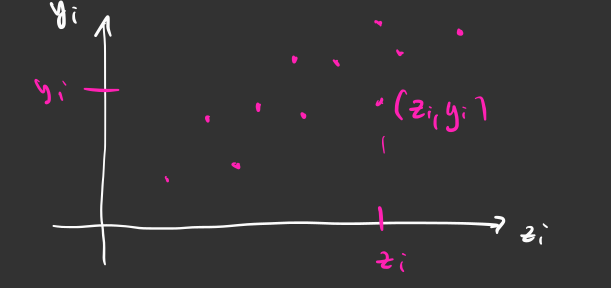
\includegraphics[width=0.5\linewidth]{curve-fitting}
	}
\end{frame}
\begin{frame}
	\Hide{	\textbf{Question:}
		Is there a ``significant'' relation between the $z_i$ and $y_i$?\\~\\
		Let us consider the $z_i$ as input (independent/explanatory/exogenous) variable,\\
		and the $y_i$ as output (dependent/predicted/response...) variable.\\~\\
		{Examples: $z_i$ = (temperature, light intensity), $y_i$ = plant height or $z_i$ = year, $y_i$ = global mean temperature}\\
		~\\~\\
		\textbf{Mathematically asking:} Is there a function $f$, so that
		$
		f(z_i)\cong y_i~\text{ for all $i=1,\ldots,m$?}
		$
		~\\~\\~\\
		\begin{minipage}[t]{0.48\textwidth}
			\underline{Exact fit:} \textbf{Interpolation}\\
			$$f(z_i)=y_i~\forall i=1,\dots,m$$
			~\\
			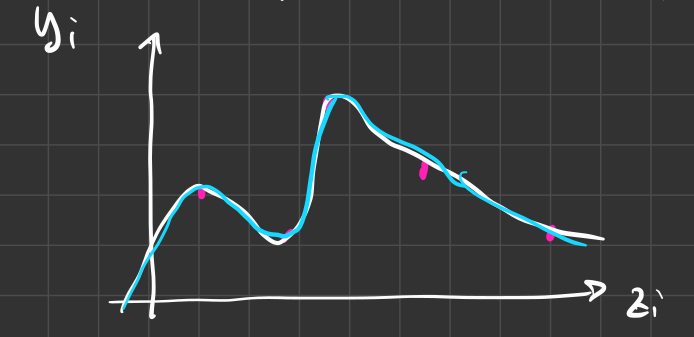
\includegraphics[width=0.7\linewidth]{interpolation-hand}
		\end{minipage}
		\begin{minipage}[t]{0.48\textwidth}
			\underline{Approximate fit:} \textbf{Regression/Smoothing}\\
			$$f(z_i)\approx y_i~\forall i=1,\dots,m$$
			~\\
			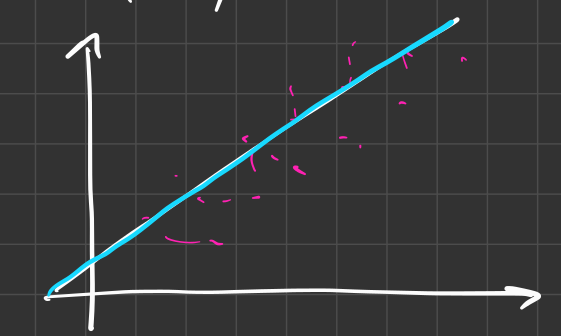
\includegraphics[width=0.7\linewidth]{regression-hand}
		\end{minipage}
	}
\end{frame}
\begin{frame}
	~\\
	\Hide{
		In order to find such a fit, we need to restrict ourselves to certain classes of functions $f$. With other words we need to assume a certain ''model'':\\
		$$z_i\stackrel{f}{\mapsto}y_i$$\\
		~\\
		In this course we will consider models of the following kind:
		$$
		f:\mathbb{R}\rightarrow\mathbb{R},~~f(z):=\sum_{k=1}^{n}x_kf_k(z)
		$$
		\begin{itemize}
			\item[$\rightarrow$] More precisely, we assume that the relation between the $z_i$ and the $y_i$ can be modeled by a \textit{linear combination}		 of $\underbrace{\text{some functions}~f_k:\mathbb{R}\rightarrow\mathbb{R}}_{\textit{\color{header}given by assumption}}$ 
			with 
			$\underbrace{\text{some coefficients/parameters}~x_k}_{\color{header}\textit{to be determined}~(f(z_i)\cong y_i)}$
			\item [] {\small (More generally $f,f_k\colon \R^k \to \R$. Important here is the fact that our model $f$ is linear combined from the $f_k$.)}
		\end{itemize}
		~\\
		\begin{example}[Polynomial Interpolation/Regression]
			One often considers a polynomial model:
			$$
			f_k(z) := z^{k-1},~~\text{so that}~~f(z)=x_1+x_2z+x_3z^2+\dots+x_nz^{n-1}
			$$
			For example, if $n=2$ then $f(z)=x_1+x_2z$ (an affine linear model).
		\end{example}
	}
\end{frame}

\begin{frame}
	~\\
	\Hide{
		\textbf{How does this translate into a linear system ``$Ax \cong b$''?}\\
		~\\
		For all measurements $(z_1,y_1),\dots,(z_m,y_m)$ we require:
		$$
		\sum_{k=1}^{n}x_kf_k(z_i)=f(z_i)\cong y_i~~\text{for all}~i=1,\dots,m
		$$
		Writing these equations row by row for each $i$-th measurement gives:
		\begin{align*}
		&\begin{matrix}
		i=1:&x_1f_1(z_1)+x_2f_2(z_2)+\dots+x_nf_n(z_1)&=y_1\\
		\vdots&\vdots&\vdots\\
		i=m:&x_1f_1(z_m)+x_2f_2(z_m)+\dots+x_nf_n(z_m)&=y_m
		\end{matrix}
		\end{align*}
		Using matrix notation, this system can be written as:
		$$
		\underbrace{
			\begin{pmatrix}
			f_1(z_1)&\cdots&f_n(z_1)\\
			\vdots&\ddots&\vdots\\
			f_1(z_m)&\cdots&f_n(z_m)
			\end{pmatrix}}_{=:A\in\mathbb{R}^{m\times n}}
		\underbrace{\begin{pmatrix}x_1\\x_2\\\vdots\\x_n\end{pmatrix}}_{=:x\in\mathbb{R}^n}
		\cong\underbrace{\begin{pmatrix}y_1\\\vdots\\y_m\end{pmatrix}}_{=:b\in\mathbb{R}^m} 
		~~~\Leftrightarrow~~~
		Ax\cong b
		$$
		~\\
		$\rightarrow$ Also revisit Example \ref{ex:interpolation}.
	}
\end{frame}

\begin{frame}
	~\\
	\Hide{
		\begin{minipage}[t]{0.48\textwidth}
			\underline{Exact:} \textbf{Interpolation}
			$$
			Ax=b
			$$
		\end{minipage}
		%%
		\begin{minipage}[t]{0.48\textwidth}
			\underline{Approximate:} \textbf{Regression}
			$$
			Ax\approx b
			$$
			A common approach to address a regression problem is a linear least squares formulation:
			\begin{align*}
			\min_{x\in\mathbb{R}^n}~\|Ax-b\|_2^2 ~&=~\sum_{i=1}^m(Ax-b)_i^2\\
			&=~\sum_{i=1}^m(f(z_i)-y_i)^2
			\end{align*}
			~\\
			\begin{figure}
				\centering
				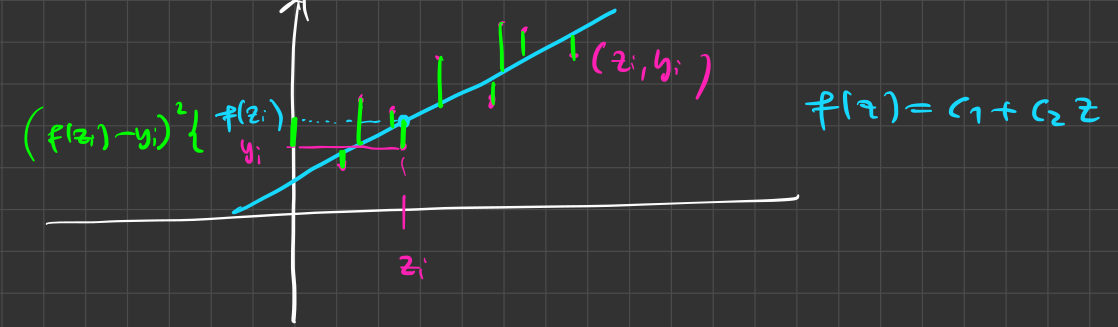
\includegraphics[width=1.1\linewidth]{regression-linear}
			\end{figure}
			
		\end{minipage}
		
		
	}
\end{frame}

\begin{frame}
	\Subsubsection{Existence and Uniqueness Analysis}
	\Hide{
		Let us consider the following cases:\\
		\begin{figure}
			\centering
			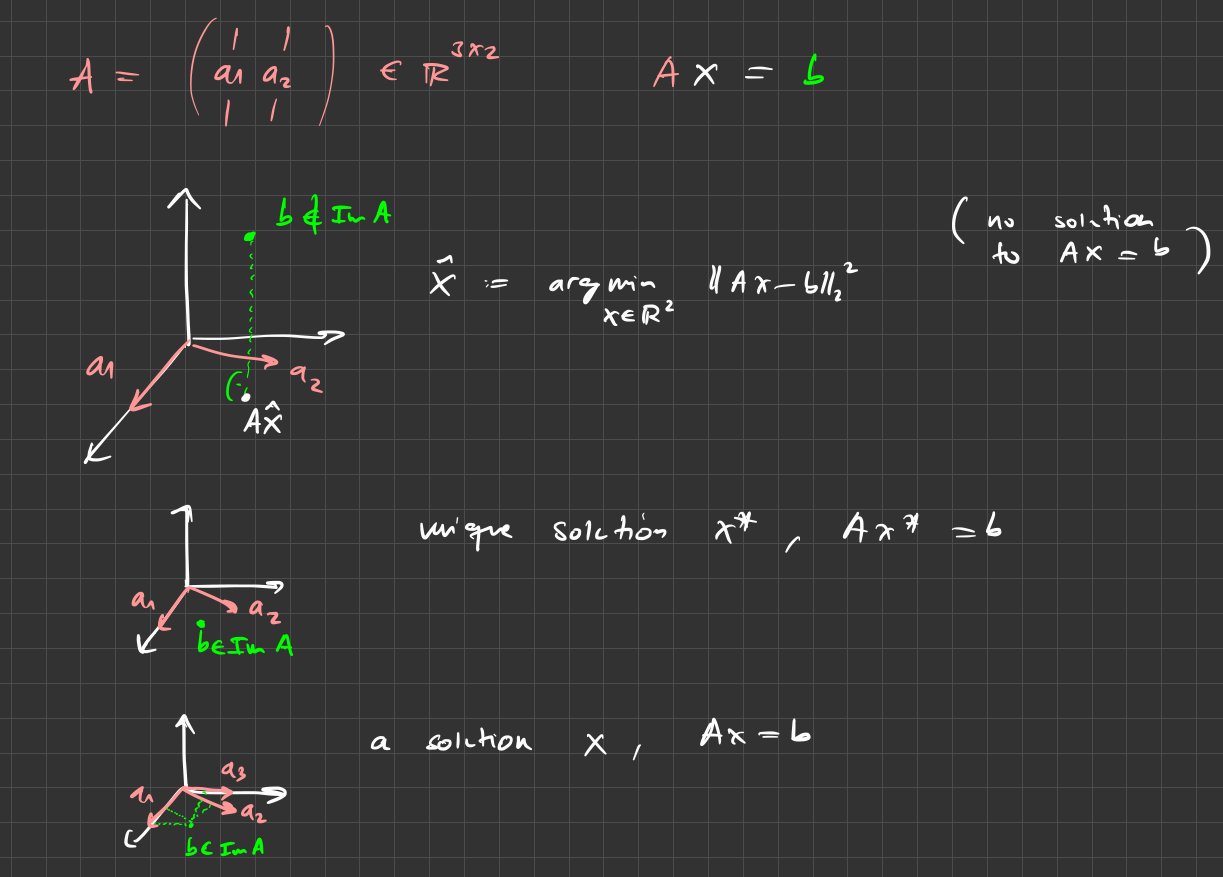
\includegraphics[width=0.85\linewidth]{existence-uniqueness-linsys}
			%	\caption{}
			%	\label{fig:existence-uniqueness-linsys}
		\end{figure}
		
		
		
	}
\end{frame}
\begin{frame}
	\textit{Summary}\\~\\
	\textbf{Aim:} \vspace*{-0.5cm}
	\begin{center}
		\textit{Given $A\in\mathbb{R}^{m\times n}$ ($m\neq n$ possible) and $b\in\mathbb{R}^m$,
			find $x\in\mathbb{R}^n$ such that\\
			$Ax=b.$}
	\end{center}
	\Hide{Here:
		\begin{itemize}
			\item[$m$]$=~\sharp$ equations $=~\sharp$ measurements $=$ length of the column vectors\\
			\item[$n$]$=~\sharp$ unknowns $=~\sharp$ parameters $=~\sharp$ columns\\
		\end{itemize}
		~~~~~~$\begin{matrix}~&{\color{cyan}n}\\A=~{\color{cyan}m}&\begin{pmatrix}|&~&|\\a_1&\cdots&a_n\\|&~&|\end{pmatrix}\end{matrix}$,~~~with image Im$(A)=\{Ax:\in\mathbb{R}^n\}~=$ span$(a_1,\dots,a_n)$\\
		~\\~\\
		Let us define the solution set
		$$S:=\{x\in\mathbb{R}^n:Ax=b\}~=~f_A^{-1}(\{b\}),$$
		then there are three possible states, namely,
		$$
		|S|=~\begin{cases}
		&0~:~\text{``no solution'', if~~}b\notin\text{Im}(A)\\
		&1~:~\text{``unique solution'', if~~}b\in\text{Im}(A)~\text{and independent columns}~(\text{ker}(A)=\{0\})\\
		&\infty~:~\text{``infinitely many solutions'', if~~}b\in\text{Im}(A)~\text{and dependent columns}~(\text{ker}(A)\neq\{0\})
		\end{cases}
		$$
		For a given $b$, observe the relations between image and existence as well as kernel and uniqueness. In fact,
		$b\in$ or $\notin\text{Im}(A)$ decides if solutions \textbf{exist} and \text{ker}(A) $=$ or $\neq~\{0\}$ gives the solutions' \textbf{uniqueness}.}
\end{frame}
%
%
\begin{frame}
	\Hide{
		Quick clarification:\\~\\
		Let $\ker(A)\neq \{0\}$, then there exists a $w \in \Rn$ so that $$A (\alpha w)= 0$$ for \textit{all} scalars $\alpha \in \R $.\\~\\
		If $b\in\im(A)$, then there exists an $x \in \Rn$, so that $$Ax = b.$$
		Adding these two equations gives
		$$A(x + \alpha w) = b ~~~\forall \alpha \in \R .$$ 
		With other words, we find infinitely many solutions.\\~\\
		Another equivalent argument in view of Lemma \ref{lem:linear-independence}: A nontrivial kernel implies that the columns are linearly dependent and thus vectors in their span are not uniquely combined. Now we see that this already implies infinitely many ways to linearly combine the columns of $A$ to obtain $b$ (assumed $b$ lies in there span).
	}
\end{frame}


\begin{frame}
	\Subsection{More on Image and Kernel}
Let us fix $\F = \R$ in this section. In this subsection we derive some more results on the kernel 
	$$\ker(A) = \{x\in \Rn: Ax = 0\} \subset \Rn$$ 
	and the image 
	$$\im(A) = \{Ax: x \in \Rn \} \subset \Rm.$$ 
 These results prove useful in later sections; in particular when we talk about the singular value decomposition.
	~\\~\\~\\
	\textbf{The Four Fundamental Subspaces}\\~\\
	In the context of a matrix $A \in \Rmn$ there are four subspaces that stand out:
	\begin{align*}
	  \ker(A)  ~~~\bot~~~&\im(A^\top)\\
	  \im(A) ~~~\bot~~~&\ker(A^\top).
	\end{align*}
	\Hide{The big picture of linear algebra:\\
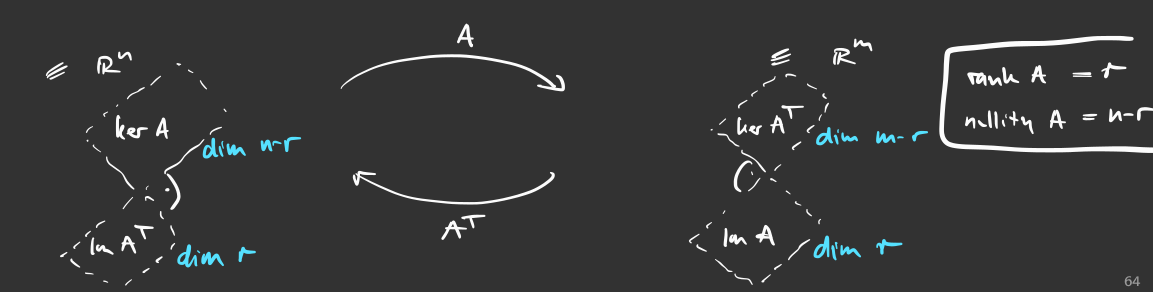
\includegraphics[width=0.9\linewidth]{media/bigpic-la}
}	
\end{frame}

\begin{frame}
\begin{example}\label{ex:bigPicture-LA}
		Let us consider
	$$A = \begin{pmatrix}1&2\\3&6\end{pmatrix}	,~~~~A^\top= \begin{pmatrix}1&3\\2&6\end{pmatrix}$$
	\Hide{
Then we find\\
\begin{minipage}[t]{0.48\textwidth} \small
\begin{align*}
\im(A) &= \text{span} \begin{pmatrix}1\\3\end{pmatrix}\\
\ker(A) &= \{x\in\R^2: Ax = 0\}\\
&= \{x\in\R^2:  x_1\begin{pmatrix}1\\3\end{pmatrix} +  x_2\begin{pmatrix}2\\6\end{pmatrix} = 0\} \\
&= \{x\in\R^2: 1x_1 + 2x_2 = 0\} \\
&= \{x\in\R^2: x_1 = - 2x_2\} \\
&= \spann \begin{pmatrix}-2\\1\end{pmatrix}
\end{align*}
\end{minipage}
\begin{minipage}[t]{0.48\textwidth} \small
\begin{align*}
\im(A^\top) &= \spann \begin{pmatrix}1\\2\end{pmatrix}\\
\ker(A^\top) &= \{x\in\R^2: Ax = 0\}\\
&= \{x\in\R^2: 1x_1 + 3x_2 = 0\}\\
&= \{x\in\R^2:  x_1 = - 3x_2 \}\\
&= \spann \begin{pmatrix}-3\\1\end{pmatrix}
\end{align*}
\end{minipage}
~\\
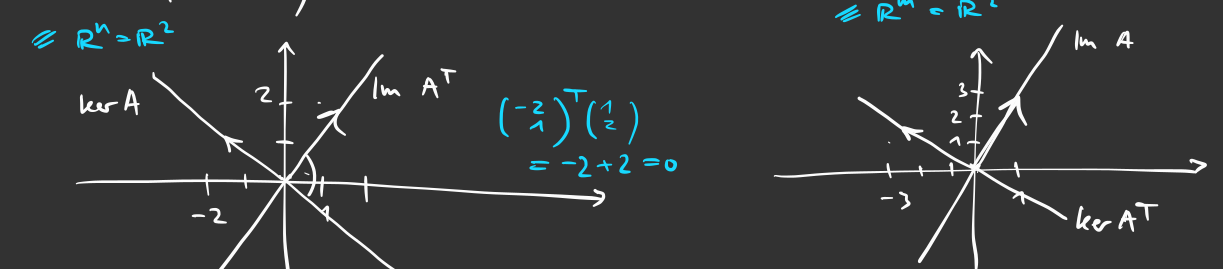
\includegraphics[width=0.9\linewidth]{media/ex-bigPicture-LA}
}
\end{example}

\end{frame}

\begin{frame}
	We need another definition:
	\begin{defi}[Orthogonal subspaces]
		 Let $U,V \subset \R^n$ be two subspaces.  
		 \begin{itemize}
		 	\item[i)] We call $U$ and $V$ \textbf{orthogonal} ($U \bot V$) if $u^\top v = 0$ for all $u \in U, v\in V$.
		 	\item[ii)] We call 
		 	$$U^\bot := \{x\in  \R^n \colon x^\top u = 0 ~~\forall ~u \in U\} $$
		 	the \textbf{orthogonal complement} of $V$ in $\Rn$.
		 \end{itemize}
	\end{defi}
~\\
 \textit{Exercise:} {\color{satzrot}Show that $(U^\bot)^\bot = U$ and $U \bot U^\bot$.}
\begin{example}\label{ex:orthogonalSubspaces}
	\Hide{~\\
i) $n=2$, $U := \text{span}({\begin{pmatrix}1\\0\end{pmatrix}}), V := \text{span}({\begin{pmatrix}0\\1\end{pmatrix}})$. Then
$$\forall u = \begin{pmatrix}u_1\\0\end{pmatrix} \in U, v= \begin{pmatrix}0\\v_2\end{pmatrix}\in V: u^\top v = u_1 \cdot 0 + 0 \cdot v_2 = 0. $$
Thus, $U \bot V$.
~\\
ii) $n=3$, $U := \text{span}(\begin{pmatrix}1\\0\\0\end{pmatrix}, \begin{pmatrix}0\\1\\0\end{pmatrix})$.
%Then  $U= \im(A)$ with $A = \begin{pmatrix}1&0\\0&1\\0&0\end{pmatrix} $. 
Thus for any $u\in U$ we have $u =  \begin{pmatrix}u_1\\u_2\\0\end{pmatrix}$. Then
\begin{align*}
U^\bot &= \{x\in  \R^3 \colon x^\top u = 0 ~~\forall ~u \in U\} 
 =  \{x\in  \R^3 \colon x_1u_1 + x_2u_2 = 0 ~~\forall ~u_1, u_2 \in \R \} \\
 &=  \{x\in  \R^3 \colon x_1=x_2=0 \} ~~~~\text{\color{cyan}\it(choose $u_1=1, u_2=0$ and $u_1=0, u_2=1$)}\\
 &= \text{span}(\begin{pmatrix}0\\0\\1\end{pmatrix}).
\end{align*}
\demo{draw pictures}
}
\end{example}

\end{frame}

\begin{frame}
	We now prove the orthogonality relation between the four fundamental subspaces:
\begin{lemma}\label{lem:ortho-fundamental-subspaces}
	Let $A \in \Rmn$. Then
		\begin{align*}
	\im(A)^\bot =\ker(A^\top)~~~\text{and}~~~\ker(A)^\bot=\im(A^\top)	.
	\end{align*}
	In words, $\ker(A^T)$ is the \textbf{orthogonal complement} of $\im(A)$ in $\Rm$ and $\im(A^T)$ is the orthogonal complement of $\ker(A)$ in $\Rn$.
\end{lemma}
\Hide{ 
\begin{proof}
We show the first equation. The orthogonal complement of $\im(A)$ can be characterized as
\begin{align*}
\im(A)^\bot = \{y\in\Rm: z^\top y = 0 ~~\forall z \in \im(A)\} = \{y\in\Rm: x^\top A^\top y = 0 ~~\forall x \in \Rn\}.~~~~\text{\small\it \color{cyan}(simply write $z = Ax$)}
\end{align*}	
Now we show mutual subset relation. First,
\begin{align*}
y \in \im(A)^\bot &\Rightarrow \forall x\in \Rn: x^\top(A^\top y) = 0\\
&\Rightarrow \text{for the basis vectors~} e_1,\ldots, e_n:    e_i^\top(A^\top y) = (A^\top y)_i = 0\\
&\Rightarrow   A^\top y = 0~\text{,i.e.,}~~y\in\ker(A^\top).
\end{align*}
Second, 
\begin{align*}
y \in \ker(A^\top) &\Rightarrow  A^\top y = 0\\
&\Rightarrow \forall x\in \Rn: x^\top(A^\top y) = (Ax)^\top y= 0\\
&\Rightarrow y \in \im(A)^\bot.
\end{align*}
The second equation follows from applying the first equation to  $C = A^T$ and $(U^\bot)^\bot = U$.
\end{proof}
}
% 
%We have that $\ker(A^T)$ is the \textbf{orthogonal complement} of $\im(A)$ in $\Rm$ and we write
%$$ \im(A)=\ker(A^T)^\bot ~~~\text{or}~~~\im(A)^\bot = \ker(A^T).$$
%Analogously $\ker(A)$ is the orthogonal complement of $\im(A^T)$ in $\Rn$ and we write
%$$\ker(A) = \im(A^T)^\bot~~~\text{or}~~~\ker(A)^\bot = \im(A^T).$$ 
\end{frame}

\begin{frame}
	In terms of the transpose matrix we find two more characterizations of the image and kernel:
	\begin{lemma}\label{lem:kernel-image}
			Let $A \in \Rmn$. Then
		\begin{align*}
		i)~~~\ker(A) &= \ker(A^\top A)~~~(\text{and}~~~\ker(A^\top) = \ker(AA^\top )),\\
		ii)~~~\im(A) & = \im(A A^\top)~~~(\text{and}~~~\im(A^\top) = \im(A^\top A)).
 		\end{align*}
	\end{lemma}
\Hide{
\begin{proof}
We only prove i) here. We show this by mutual subset relation:
\begin{itemize}
	\item \underline{``$\ker(A)\subseteq \ker(A^TA)$'':}\\
Let $x\in \ker(A) \stackrel{\textcolor{cyan}{\text{Def.}\ \ker(A)}}{\Rightarrow}Ax=0\Rightarrow A^TAx=0\stackrel{\textcolor{cyan}{\text{Def.}\ \ker(A^TA)}}{\Rightarrow}x\in \ker(A^TA)$.\\~\\
\item \underline{``$\ker(A^TA)\subseteq \ker(A)$'':}\\
Let $x\in \ker(A^TA) \stackrel{\textcolor{cyan}{\text{Def.}}}{\Rightarrow}A^TAx=0\Rightarrow \underbrace{x^TA^TAx}_{\textcolor{cyan}{=\|{Ax}\|_2^2}}=0 \stackrel{\textcolor{cyan}{\text{norm}~ \|{\cdot}\|_2~ \text{is definite}}}{\Rightarrow}Ax=0 \stackrel{\textcolor{cyan}{\text{Def.}}}{\Rightarrow}x\in \ker(A)$.
\end{itemize}
Exercise: To prove ii) one can exploit the orthogonality of the subspaces as derived above.\\ 
The results for the transpose follow by applying the results to $C:=A^T$.
\end{proof}
}
{
~\\
\small 
\textbf{Remark}\\
The so-called Gram matrix $A^\top A$ plays a crucial role in many applications and also analysis, for instance
\begin{itemize}
	\item it plays a key role to derive the singular value decomposition
	\item it is the system matrix in the normal equation $A^\top A x=A^\top x $ for solving least squares problems
	\item in graph theory it appears as graph Laplacian
	\item if $A \approx \nabla$ (gradient), then $A^\top\approx \text{div}$ (divergence) and $A^\top A \approx \Delta$ (Laplacian)
\end{itemize}
}
\end{frame}

\begin{frame}
	A generalization of this result is given by the following lemma.
		\begin{lemma} \label{lem:kerImProducts}
		Let $A \in \Rmn$. Then
\begin{itemize}
	\item[i)] For a matrix $B \in \R^{\ell\times m}$ with $\ker(B) = \{0\}$ 
	%$m \leq \ell$ and $\rank(B)=m$ 
	(``injective'') we have
				$$\ker(BA) = \ker(A). $$
	\item[ii)] For a matrix $C \in \R^{n\times k}$ with $\im(C)=\R^n$
	% $n \leq k$ and $\rank(C)=n$ 
	(``surjective'') we have
$$\im(AC) = \im(A). $$
\end{itemize}
	\end{lemma}

	\Hide{\small
		\begin{center}
		~\\	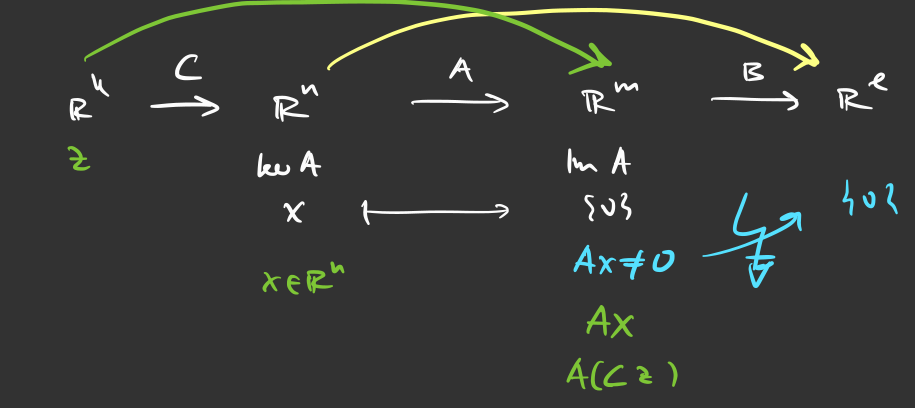
\includegraphics[width=0.4\linewidth]{media/la-concatenate-mats}\\
		\end{center}
	\begin{proof}	
We show mutual subset relation:\\
i)
\underline{``$\ker(BA)\subseteq \ker(A)$'':}\\
 	Let $BA x = B(A x) =0$. Since by assumption $\ker(B) = \{0\}$, we have $Ax = 0$.\\
	\underline{``$\ker(A)\subseteq \ker(BA)$'':}\\
	For $Ax = 0$ we also have $BAx = B(Ax)= B 0 = 0$.\\
ii)	
\underline{``$\im(AC)\subseteq \im(A)$'':}\\
Let $y = ACx = A (Cx)$ for some $x\in \R^k$. Then with $z := Cx \in \Rn$ we see that $y = Az$ is in the image of $A$.   \\
\underline{``$\im(A)\subseteq \im(AC)$'':}\\
Let $y = Az$ for some $z\in\Rn$. Since $\im(C)=\R^n$
%$\rank(C)=n$, so that its columns form a basis for $\Rn$, 
we find some coefficients $x\in\R^k$ so that $z=Cx$. With $y = ACx$ we see that $y$ is in the image of $AC$.
\end{proof}
}
\end{frame}

\begin{frame}
\textbf{Example}
~\\~\\
%\Hide{	
	The typical context to apply Lemma \ref{lem:kerImProducts} occurs when we have a decomposition of a matrix $A$ and want to investigate its kernel and its image.
	~\\~\\
	 For example, consider the reduced QR decomposition $A = QR$, where $Q \in \Rmn$ contains orthonormal columns and $R \in \Rnn$ is upper triangular. Suppose that $A$ has full rank, i.e., $\rank(A)= n$, so that $R$ is invertible (in particular $\rank(R)=n$ and $\ker(R)=\{0\}$). We thus find by Lemma \ref{lem:kerImProducts} i) that
	$$\ker(A) = \ker(QR) = \ker(R) = \{0\} $$
	and by Lemma \ref{lem:kerImProducts} ii) that
	$$\im(A) = \im(QR)= \im(Q).$$
	With other words, the $n$ columns in $Q$ are an orthonormal basis for the image $\im(A)$ of $A$.
%}
\end{frame}





% solving linear systems
\only<presentation>{\setnextsection{2}}
\lecture{Solving Linear Systems (Direct Methods)}{sollinsys}
% !TeX spellcheck = en_US


\begin{frame}
	Recommended reading:\\
	\begin{itemize}
		\item Lectures in \cite{TreBau}: 6,7,8 for $QR$; 20,21 for $LU$; 23 for $LL^\top$
		\item Section I.4 in \cite{StrangData}
		\item Sections 2.6, 2.7 in \cite{StrangLA_intro}
	\end{itemize}
	~\\~\\
	\textbf{References}
	\bibliographystyle{plain}
	\bibliography{../information/literature}
\end{frame}

\begin{frame}
	
	\Section{Solving Linear Systems with Direct Methods}
	
	\textbf{Aim:}
		\begin{center}
		\textit{	Given $A\in\mathbb{R}^{m\times n}$ ($m\neq n$ possible) and $b\in\mathbb{R}^m$,
			find $x\in\mathbb{R}^n$ such that\\
			$Ax=b.$}
	\end{center}
\Subsection{The Idea of ``Factor and Solve''}
A general theme in numerical mathematics is to reduce the general (possibly complicated) problem to one or more simpler problems with the help of transformations for which the property of interest is an invariant.\\~\\\small
\Hide{	\textbf{Simple cases:}\\ 
	\begin{itemize}
			\item $A = D =  \text{diag}(d_1,\ldots, d_n)$ diagonal
			\item $A = L$ (or $A = U$) lower (or upper) triangular system\\
			$\rightarrow$ backward/forward substitution (exercise!)\\
			\item $A = Q$ orthogonal \\
			$\rightarrow$ $A^{-1} = Q^\top$ \\
			\item $A$ has special structure: tridiagonal/banded, Toeplitz, circulant,...
		\end{itemize}
~\\
\textbf{General case:}\\
\begin{itemize}
	\item[] Assume $A = F_1   \cdots F_k$, where each factor $F_i \in \{D, L, U, Q\}$, then formally
	$$ x = F_k^{-1}\cdots F_1^{-1} b,$$
	where each solving step $F_i^{-1}$ can easily be performed.\\~\\
\end{itemize}

{\small (\textit{Remark:} ``direct'' $=$ finitely many steps to obtain the solution (typically operating on dense arrays))}\\~\\}
\end{frame}

\begin{frame}
	~\\		
	\textbf{Separate: Factorization and Solution!}\\
	~\\	
	\begin{itemize}
		\item Since the \textit{factorization} (\textit{elimination/triangularization/orthogonalization}) step is typically much more expensive than the \textit{solution} step, it makes sense to perform them separately, if the same matrix $A$ is used for multiple right-hand sides $b$.\vspace{0.5cm}
		\item The number of factors in a decomposition is the number of systems to be solved in the \textit{solution} step.\vspace{0.2cm}
		From the factors we may also gain information about the
		\begin{itemize} \normalsize
			\vspace{0.15cm}\item the image and kernel of $A$
			\vspace{0.15cm}\item \text{invertibility} of the matrix $A$ in case $m=n$ 
			\vspace{0.15cm}\item \text{solvability} of the system (i.e., the cardinality $|S|$ of the solution set $S$)
		\end{itemize} \vspace{0.5cm}
		\item We will have a look at the following decompositions
		\begin{itemize} \normalsize
			\item $A = QR$ (two systems to be solved)
			\vspace{0.15cm}\item $A = P^TLU$ (three systems to be solved)
			\vspace{0.15cm}\item $A = LL^T$ (two systems to be solved)
		\end{itemize} 
	\end{itemize}
\end{frame}

\begin{frame}
	~\\~\\
		\textbf{Never compute the inverse!}~\\~\\
	\begin{itemize}
		\item There are only very rare occasions, where an inverse matrix $A^{-1}$ is needed. In most cases, one needs inverse matrix times a vector, i.e., $A^{-1}b$.	\vspace{0.2cm} 
		\item For computing the inverse of an $(n \times n)$-matrix $A$ we have to solve $n$ linear systems:\\
		\Hide{
		\begin{equation}\label{eq:compute-inverse}
		  A \cdot [x_1,\ldots, x_n]  = \idMat,
		\end{equation}
		where the $x_j \in \Rn$ are the unknown columns of the inverse of $A$. In practice, this is typically done by computing a factorization of $A$, which is then used to solve these $n$ linear systems in \eqref{eq:compute-inverse} (see, e.g., the LAPACK routine \texttt{getri}).}
		\vspace{0.5cm}		
		\item Thus, never do
		$$\texttt{ x = inv(A) @ b}$$ instead of
		$$\texttt{ x = solve(A, b)}.$$
	\end{itemize}
\end{frame}


\begin{frame}[c]
\hspace*{1.5cm}	\Subsection{The Gram-Schmidt Algorithm and the $QR$ decomposition}
\end{frame}	

\begin{frame}
\Subsubsection{Projectors}	 
For a fixed vector $x \in \Rn\setminus\{0\}$ we have derived the orthogonal projection onto its span by
\begin{equation*}
 \text{proj}_x(y) 
 = \frac{x}{\|x\|_2} \cdot \frac{x^\top y}{\|x\|_2}
 =  \frac{xx^\top}{x^\top x} \cdot y
 =: P_x y,
\end{equation*}
where $P_x := \frac{xx^\top}{x^\top x}\in \Rnn$.\\
~\\
\Hide{We now collect some properties of this matrix:
\begin{itemize}
	\item $\im(P_x) = \spann(x)$ (note that all columns are multiples of $x$) and thus $\rank(P_x) = 1$
	\item $P_x$ orthogonally projects a vector $y \in \Rn$ onto the linear subspace $\im(P_x)= \spann(x)$
	\item Idempotent: 
	$$P_x^2 := P_x\cdot P_x = \frac{xx^\top}{x^\top x} \cdot \frac{xx^\top}{x^\top x} = \frac{x(x^\top x) x^\top}{(x^\top x)^2}  = \frac{xx^\top}{x^\top x} = P_x .$$
	  $\rightarrow$ In words: Projecting multiple times is the same as projecting once. \\~\\
	  We make this a definition:
	  \begin{definition}[Projector] \label{def:projector}
	   A matrix $P \in \Rnn$ is called \textbf{projector} if $P^2=P$.
	  \end{definition}
\end{itemize}}
\end{frame}



\begin{frame}
	\Hide{
	\begin{example}[Projectors]~\\
		\begin{itemize}
			\item $x = (1,0)^\top, P_x = ...$
			\item $x= (1,1)^\top, P_x = ...$
			\item For $\alpha\in\R$ consider $P_\alpha =\begin{pmatrix}
				1 & \alpha\\
				0 & 0
			\end{pmatrix}$  (exercise sheet)
		\end{itemize}
	\end{example}
}
\end{frame}


\begin{frame}
	For any projector $P \in \Rnn$ we can show: 
	\begin{lemma}[Projector Properties]\label{lem:projector}
		Let  $P \in \Rnn$ be such $P^2 = P$, then
		\begin{itemize}
			\item[i)] \color{satzrot}$\im P = \ker (I-P)$,
			\item[ii)] \color{satzrot}$\ker(P) \cap \ker(I-P) = \{0\} $,
			\item[iii)] $(I-P)$ is also a projector,
			\item[iv)] $\forall y \in \Rn~ \exists_1 v \in \im(P), r \in \im(I-P)\colon ~y = v +r $,\\
			with other words, the mapping $\im(P) \times \im(I-P) \to   \Rn, (v,r) \mapsto v +r$ is bijective.
		\end{itemize}
	\end{lemma}
\Hide{	\begin{proof}~\\ 
		\begin{itemize}
			\item[i)] $\subseteq$: For $y=Px$ we find $(I-P)y = Px - P^2x = 0$.\\
			$\supseteq$: For $y \in  \ker(I-P)$ we have $y = (I-P + P)y = 0 + Py \in \im(P)$. 
			\item[ii)] Let $Px = 0 $ and $(I-P)x = 0$, then $x = (I-P + P)x = 0 + 0 = 0$.
			\item[iii)] $(I-P)^2 = I - 2P + P^2 = I -2P+P = I-P$.
			\item[iv)] Let $y \in \Rn$.\\
			Existence: Choose $v=Py \in  \im(P)$ and $r=(I-P)y \in \im(I-P)$, then we find 
			$$  v +r = Py + (I-P)y = y .$$
			Uniqueness: We assume there is another pair $\tilde{v} \in \im P= \ker(I-P)$ and $\tilde{r}\in \im(I-P)=\ker(P)$ with $y = \tilde{v} + \tilde{r}$. Since the kernel of matrix is a linear subspace (therefore closed under linear combinations), also $(v- \tilde{v})\in\ker(I-P)$ and $(r- \tilde{r})\in\ker(P)$. Now observe
			$0 = y-y = v- \tilde{v} + r -\tilde{r}. $
			Multiplying with $P$ yields
			$$0 = P(v- \tilde{v}) + P(r -\tilde{r})= P(v- \tilde{v}) ~~~\Rightarrow ~~~(v- \tilde{v}) \in \ker(P) \cap \ker(I-P) = \{0\} . $$
			Multiplying with $I-P$ yields
			$$0 = (I-P)(v- \tilde{v}) + (I-P)(r -\tilde{r})= (I-P)(v- \tilde{v}) ~~~\Rightarrow ~~~(r -\tilde{r}) \in \ker(I-P) \cap \ker(P) = \{0\}  .$$
			Thus $v = \tilde{v}$ and $r = \tilde{r}$. 
		\end{itemize}
	\end{proof}} 
\end{frame}


\begin{frame}
Remark:\\~\\ In view of Lemma \ref{lem:projector} iv) we say that $\Rn$ is the direct sum of the subspaces $\im(P)$ and $\im(I-P)$. Each vector $y \in \Rn$ uniquely splits into the additive components $v$ and $r$. Due to i) and iii) of this lemma, also the same is true for the subspaces  $\im(P)$ and $\ker(P)$.\\
~\\
\Hide{We now continue with properties of $P_x$:
Symmetry: $$P_x^\top = \frac{(xx^\top)^\top }{x^\top x}  = \frac{(x^\top)^\top x^\top }{x^\top x} = \frac{xx^\top}{x^\top x} = P_x .$$\\~\\
	 In general we define:
	\begin{definition}[Orthogonal Projector] \label{def:ortho-projector}
	A matrix $P \in \Rnn$ is called \textbf{orthogonal projector} if $P^2=P$ and $P^\top = P$. 
	\end{definition}	
For any orthogonal projector (such as $P_x$) one can show:
\begin{lemma}[Orthogonal Projector Properties]\label{lem:ortho-projector}
	Let  $P \in \Rnn$ be such $P^2 = P$ and $P^\top = P$, then
	$$\im P \bot  \im (I-P).$$
\end{lemma}
\begin{proof}
	From Lemma \ref{lem:projector} and Lemma \ref{lem:ortho-fundamental-subspaces} (1.45) as well as the symmetry of $P$ (and thus $I-P$) we find
	$$ \im(P) = \ker(I-P) = \ker((I-P)^\top) = \im(I-P)^\bot .$$
\end{proof}
In view of Lemma \ref{lem:projector} iv) we find for an orthogonal projector, that the  components $v \in \im( P)$ and $r \in \ker(P)$ are orthogonal to each other.} 
\end{frame}


\begin{frame}
\textbf{Orthogonal Projection with Orthonormal Basis}\\~\\
Let us now consider more than just one vector. In fact, let $q_1,\ldots, q_r \in \Rm$ be orthonormal; thus $r \leq m$. Then let us define the matrices
\begin{align*}
 \widehat{Q} &:= [q_1,\ldots, q_r] \in \R^{m \times r},\\
 P:=&P_{q_1,\ldots, q_r } := \widehat{Q}\widehat{Q}^\top  \in \Rmm.
\end{align*}
Attention: For $r < m$, $\widehat{Q}$ is not an orthogonal matrix and thus $ P = \widehat{Q}\widehat{Q}^\top \neq I$ in general. However, for the Gramian matrix which collects all possible pairs of inner products we have $ \widehat{Q}^\top\widehat{Q} = I$ ($\widehat{Q}^\top$ is only a left-inverse).\\~\\
\Hide{We find the following properties of $P=P_{q_1,\ldots, q_r }$:
\begin{itemize}
	\item Sum of rank--one (orthogonal) projectors:\\
	 $$ P= \sum_{j=1}^r q_j q_j^\top = \sum_{j=1}^r P_{q_j} .$$
	 \item Orthogonal projector:
	 \begin{align*}
	  & P^2 = \widehat{Q}(\widehat{Q}^\top\widehat{Q})\widehat{Q}^\top = \widehat{Q}\widehat{Q}^\top = P\\
	  & P^\top = (\widehat{Q}\widehat{Q}^\top)^\top = (\widehat{Q}^\top)^\top\widehat{Q}^\top = P
	 \end{align*}
	 \item $P$ projects on the image of $\widehat{Q}$:
	 In fact, by Lemma \ref{lem:kerImProducts} (1.47) ii) (with $\im(\widehat{Q}^\top)=\R^r$) we find
	  $$\im(P) = \im(\widehat{Q}\widehat{Q}^\top) = \im(\widehat{Q}).$$
	  In particular: $\rank(P) = r$.
\end{itemize}}
\end{frame}

\begin{frame}
\Hide{	\begin{itemize}
		\item By Lemma \ref{lem:projector} i)+iii) and Lemma \ref{lem:kerImProducts}(1.47) i) (with $\ker(\widehat{Q}) = \{0\}$) we find 
	     \begin{align*}
	          \im (I-P) = \ker(P) = \ker(\widehat{Q}\widehat{Q}^\top) = \ker (\widehat{Q}^\top) 
	     \end{align*}
	    \item In Lemma \ref{lem:ortho-projector} we recover Lemma \ref{lem:ortho-fundamental-subspaces} (1.45):
	    \begin{align*}
	     \im(P)\bot  \im (I-P)
	      ~~~\Leftrightarrow ~~~ 
	      \im(\widehat{Q}) \bot \ker (\widehat{Q}^\top) 
	    \end{align*}
		\item By Lemma \ref{lem:projector} iv) we have 
		\begin{align*}
		 \forall y \in \Rn~ \exists_1 v \in \im(P)=&\im(\widehat{Q}), r \in \im (I-P) =\ker(\widehat{Q}^\top)\colon\\ 
		 y &= v + r \\
		 & = Py + (I-P) y\\
		 & = \widehat{Q}\widehat{Q}^\top y + (I- \widehat{Q}\widehat{Q}^\top) y
		\end{align*}
		where $v$ is the orthogonal projection of $y$ onto $\im(\widehat{Q})$ and $r$ the orthogonal residual vector; the components are orthogonal, i.e., 
		$$(v,r) = v^\top r = 0.$$
	\end{itemize}}
\end{frame}

\begin{frame}
	\begin{example}Let us consider:\\
		$$q_1 = \frac{1}{\sqrt{2}}(1,1,0)^\top, q_2 =  \frac{1}{\sqrt{2}}(-1,1,0), y=(0,1,1)^\top  \in \R^3 $$
\Hide{		Then
		$$P = \widehat{Q} \widehat{Q}^\top = \begin{pmatrix}
		 1 & 0 & 0 \\ 0 & 1 & 0 \\ 0 & 0 & 0
		\end{pmatrix} $$
		So that for $y = (y_1, y_2, y_3)^\top \in \R$ we obtain
		$$ Py = \begin{pmatrix}
		y_1\\y_2\\0
		\end{pmatrix}= \begin{pmatrix}
		0\\1\\0
		\end{pmatrix},$$
		i.e., as expected the orthogonal projection onto the $x_1/x_2$-plane (=$\im(\widehat{Q})$).}
	\end{example}
\end{frame}
 
\begin{frame}
	 \textbf{Orthogonal Projection with Arbitrary Basis}\\~\\
	 Let $a_1,\ldots, a_n$ be linearly independent vectors in $\Rm$ ($m \geq n$) and let us put the vectors into a matrix $A = [a_1,\ldots, a_n] \in \Rmn$.\\
	 
	 \textit{How to define an orthogonal projector on the image of $A$?}\\~\\
\Hide{	 Let us first recall that $\im(A) \bot \ker(A^\top)$ by Lemma \ref{lem:ortho-fundamental-subspaces} (1.45).
	 Thus we are looking for a matrix $P \in \Rmm$ such that
	 \begin{align*}
	  &\forall b \in \Rm\colon ~Pb \in \im(A)~\text{, i.e.,} Pb = Ax~\text{for some $x$ to be determined}\\
	  &b - Pb \in \im(A)^\bot = \ker(A^\top)
	 \end{align*}
	 Combining these two gives
	 $$0 = A^\top(b - Pb)= A^\top(b - Ax)  =  A^\top b - A^\top Ax. $$
	 Then by Lemma \ref{lem:kernel-image} (1.46) i) we have $\ker(A^\top A) = \ker(A) = 0$, so that the Gram matrix $A^\top A$ is invertible, which yields
  	 $$ x = (A^\top A)^{-1}A^\top b $$
  	 and the orthogonal projection $b$ onto the image of $A$ is given by
  	 $$Ax =   A(A^\top A)^{-1}A^\top b =: Pb.$$
 	 Indeed we find, $P^2 = P$ and $P^\top = P.$ Also note that for $A=\widehat{Q}$ this collapses to $P = \widehat{Q}\widehat{Q}^\top$. Further note that this coincides with $P_x = x (x^\top x)^{-1} x^\top$.
 ~\\
 {\footnotesize -----\\ \textit{Remark: The final step to bridge between orthogonal projections and least squares, is to show the intuitive result that orthogonal projections are precisely those projections that produce the smallest residual $(I-P)b$. This is shown later in this course.}}}
\end{frame}

\begin{frame}
	\begin{example}Let us consider:\\
		$$a_1 = (1,1,0)^\top, a_2 =  (0,1,0), y=(0,1,1)^\top  \in \R^3 .$$
		We observe that $\im(A) = \im(\widehat{Q})$, so that we would expect the same projector as in the example above.\\
\Hide{		First we compute
		$$A^\top A = \begin{pmatrix}
		 2 & 1 \\ 1 & 1
		\end{pmatrix}. $$
		From $$A^\top A x = \begin{pmatrix}
		1 \\ 0
		\end{pmatrix} \Leftrightarrow x =  \begin{pmatrix}
		1 \\ -1
		\end{pmatrix} $$
		and 
		$$A^\top A x = \begin{pmatrix}
		0 \\ 1
		\end{pmatrix} \Leftrightarrow x =  \begin{pmatrix}
		-1 \\ 2
		\end{pmatrix} $$
		we find 
		$$(A^\top A)^{-1} = \begin{pmatrix}
		1 & -1 \\ -1 & 2
		\end{pmatrix}. $$
		And thus
		$$P = A (A^\top A)^{-1} A^\top =  \begin{pmatrix}
		1 & 0 & 0 \\ 0 & 1 & 0 \\ 0 & 0 & 0
		\end{pmatrix} .$$}
	\end{example}
\end{frame}

\begin{frame}
	\Subsubsection{A=QR from the (classical) Gram--Schmidt Algorithm}	
\Hide{\begin{center}
	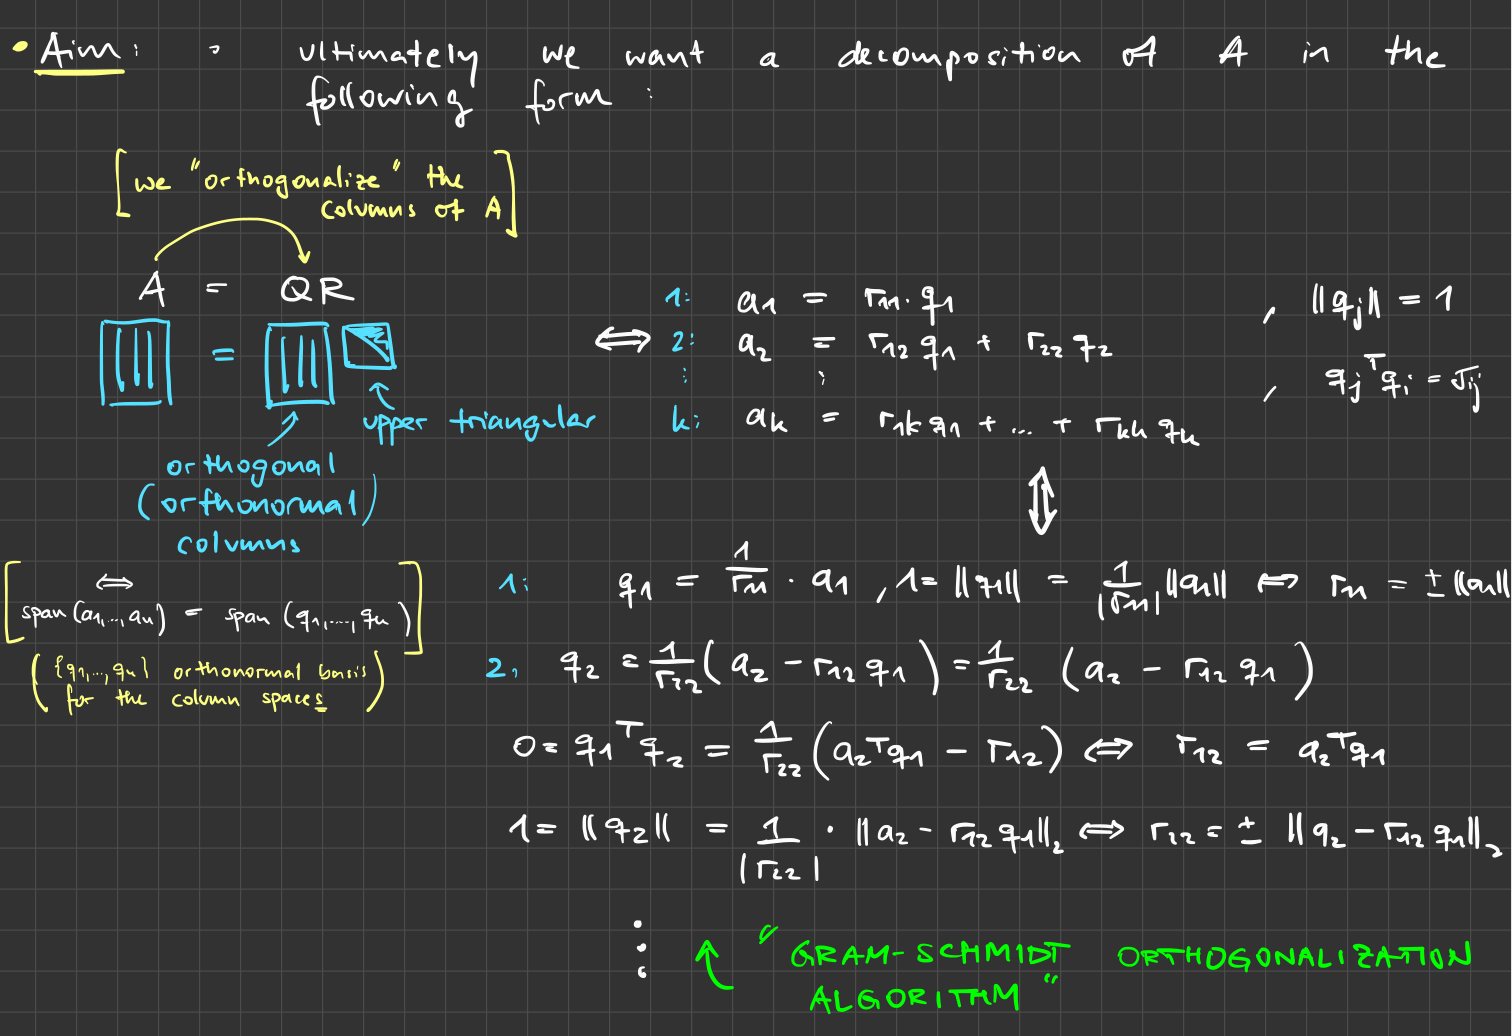
\includegraphics[width=0.94\linewidth]{content/Gram-Schmidt-Idea}
\end{center}}
\end{frame}


\begin{frame}[c]
\textbf{Classical Gram--Schmidt Orthogonalization Algorithm}\\~\\
\hspace*{1cm}
\begin{minipage}{0.8\textwidth}
\begin{algorithm}[H]
$r_{11} = \| a_1 \|$\\
$q_1 = \frac{a_1}{r_{11}}$\\
~\\
\For{ $k = 2, \dots, n$ }{ 
\For{ $\ell = 1,\dots, k-1$}{  
	$r_{\ell k} = a_k^\top q_\ell$	\\
 } 
		$\widetilde{q}_k = a_k - \sum _{\ell=1}^{k-1} r_{\ell k} \, q_\ell~~ {\color{cyan}= (I-P_{q_1,\ldots,q_{k-1}})a_k \in \im(\widehat{Q}_{k-1})^\bot}$\\
	$r_{kk} = \| \widetilde{q}_k \|$\\
	\If{$r_{kk} = 0$}{
		pick arbitrary $q_k \in \im(\widehat{Q}_{k-1})^\bot = \ker(\widehat{Q}_{k-1}^\top)$	\\
	    {\color{gray}// for example by solving $\widehat{Q}_{k-1}^\top q_k = 0$ and normalizing}
}\Else{$q_k = \frac{\widetilde{q}_k}{r_{kk}}$}
}
{\color{gray}// For full QR:}\\
Fill up columns of $\widehat{Q}:= \widehat{Q}_n$ with $(m-n)$ orthonormal vectors of $\ker(\widehat{Q}_{k-1}^\top)$\\
Fill up rows of $\widehat{R} := (r_{ij})$ with $(m-n)$ zero rows
\end{algorithm}
\end{minipage}
~\\
\textit{\color{cyan} Observation: This algorithm successively orthogonalizes the columns of $A$!}
 \end{frame}


\begin{frame}
	These ideas lead to\\
	\begin{theorem}[QR decomposition]\label{theo:qr¸}
		Let $A\in\R^{m\times n}$ with $m \geq n$, then there exists a matrix $\widehat Q\in\R^{m\times n}$ with orthonormal columns and an upper triangular matrix $\widehat R\in\R^{n\times n}$ such that
		$$A=\widehat Q \widehat R.$$
		{\color{defgruen} We call this the \textbf{\underline{reduced} QR decomposition} of $A$.}\\~\\
		One can extend the columns of $\widehat Q$ with orthonormal columns to obtain an orthogonal matrix $Q\in\R^{m\times m}$ and the rows of $\widehat R$ by zero rows to obtain a matrix $R =\begin{pmatrix}
		\widehat{R}\\0
		\end{pmatrix}\in \R^{m\times n}$ and thereby obtain
		$$A = QR .$$
		{\color{defgruen} We call this the \textbf{QR decomposition} of $A$.}
	\end{theorem}\vspace{-0.1cm}
	\Hide{
		\begin{proof}\small
		Sketch: First note that by construction $\spann(a_1,\ldots, a_k) = \spann(q_1,\ldots, q_k)$ for all $1\leq k \leq n$ and $q_1,\ldots, q_k$ orthonormal (exercise: verify this by an induction proof).\\		
		If $\ker(A) = \{0\}$ (independent columns), then for all $1\leq k \leq n$ we have $$a_k \notin \spann(a_{1},\ldots, a_{k-1}) = \spann(q_{1},\ldots, q_{k-1}) $$  and thus for the residual of the projection
		$$\widetilde{q}_k = (I-P_{q_1,\ldots,q_{k-1}})a_k\neq 0$$
		so that $r_{kk} \neq 0$. Thus the classical Gram-Schmidt algorithms produces $\widehat{Q}$ and $\widehat{R}$ so that $A = \widehat{Q}\widehat{R}$.\\
		If columns of $A$ are dependent, then there are $k$ for which 
		$$a_k \in \spann(a_{1},\ldots, a_{k-1}) = \spann(q_{1},\ldots, q_{k-1})$$ so that the residual is $\widetilde{q}_k = (I-P_{q_1,\ldots,q_{k-1}})a_k = 0$, thus we pick an arbitrary vector in $q_k \in \im(\widehat{Q}_{k-1})^\bot = \ker(\widehat{Q}_{k-1}^\top)$ and continue.
	\end{proof}}
\end{frame}
\begin{frame}
	\begin{example}~\\
\Hide{	 \begin{center}
	 	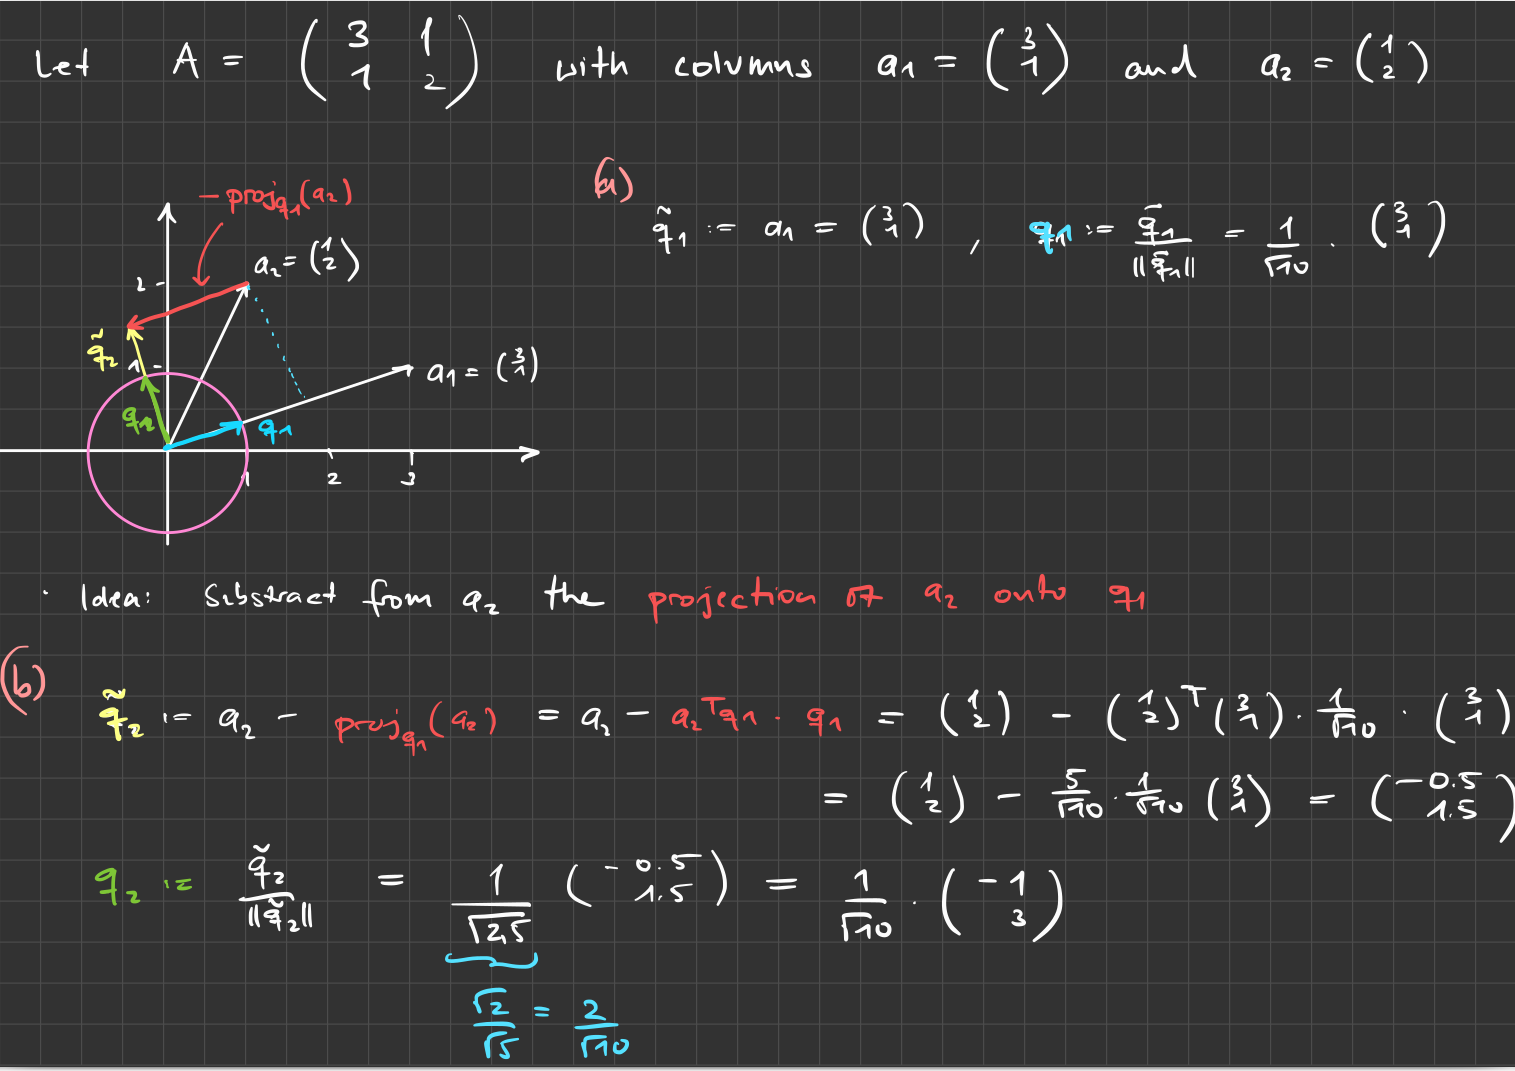
\includegraphics[width=0.95\linewidth]{content/Gram-Schmidt-Example-1}
	 \end{center}}
	\end{example}
\end{frame}
\begin{frame}
	\Hide{	 \begin{center}
		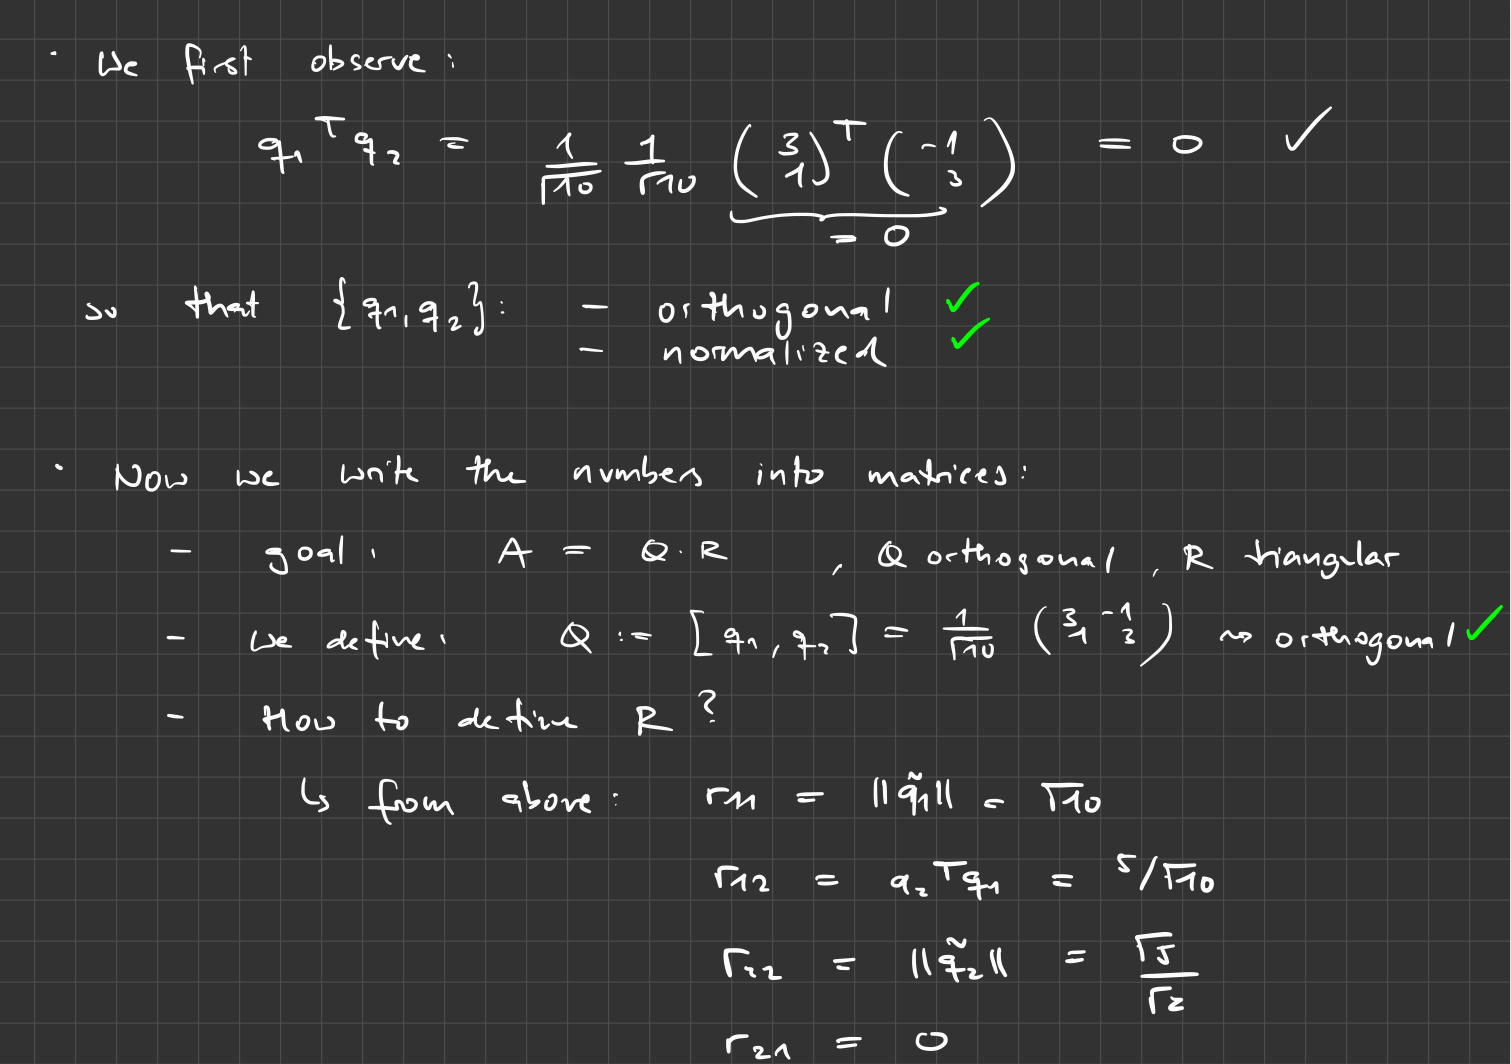
\includegraphics[width=0.95\linewidth]{content/Gram-Schmidt-Example-2}
	\end{center}}
\end{frame}
\begin{frame}
\Hide{	\begin{center}
		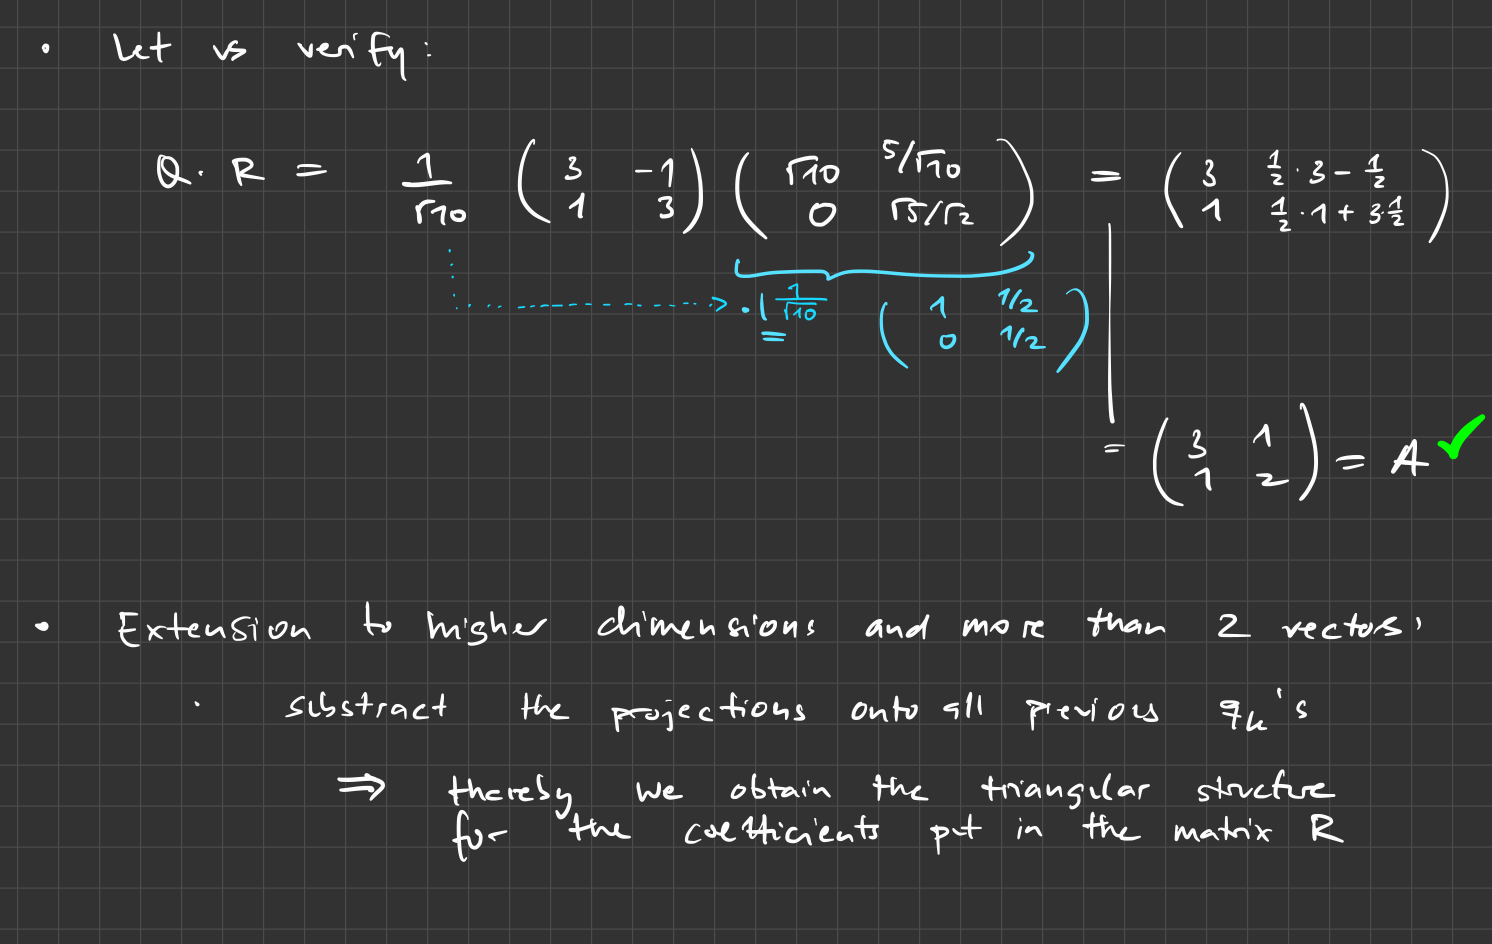
\includegraphics[width=0.95\linewidth]{content/Gram-Schmidt-Example-3}
	\end{center}}
\end{frame}





\begin{frame}
	Let $m \geq n$.\\
	~\\
	\textbf{(1) Factorization}~\\
Gram-Schmidt orthogonalization algorithm, Householder reflections or Givens Rotations can be used.\\~\\
	\textit{In Python}
	$$Q, R = \texttt{scipy.linalg.qr(A)} $$
	~\\
	\textit{or for the reduced version run }
	$$\widehat{Q}, \widehat{R}  = \texttt{scipy.linalg.qr(A, mode="economic")}$$
	~\\
	\textbf{(2) Solving}~\\
	\Hide{
	Let us consider the reduced $QR$ decomposition $\widehat{Q}\widehat{R}=A$. Then project $b$ on the image of $A$ by $\widehat{Q}\widehat{Q}^\top b$. Then we obtain the solvable auxiliary problem
		\begin{align*}
	Ax=\widehat{Q}\widehat{Q}^\top b~~\Leftrightarrow~~\widehat{Q}\widehat{R}x= \widehat{Q}\widehat{Q}^\top b~~
	\stackrel{{\color{cyan}\ker \widehat{Q} = \{0\} }}{\Leftrightarrow}~~\widehat{R}x = \widehat{Q}^\top b.
	\end{align*}
	Note that if $b \in \im(A)$ then $b= \widehat{Q}\widehat{Q}^\top b$, so that in this case we solve the original problem
	$$Ax=\widehat{Q}\widehat{Q}^\top b = b .$$
	~\\
%	 containing the first $n$ orthonormal columns of $Q$ and $\widehat{R} \in \Rnn$ with $R =\begin{pmatrix}
%	\widehat{R}\\0
%	\end{pmatrix} $. Since $\widehat{Q}^\top$ is a left--inverse of $\widehat{Q}$ (i.e., $\widehat{Q}^\top\widehat{Q} = I $), we find the  solution by
%	\begin{align*}
%	Ax=b~~\Leftrightarrow~~\widehat{Q} \widehat{R}x=b~~
%	\stackrel{{\color{cyan}\widehat{Q}^T\cdot |~,  \widehat{Q}\cdot | }}{\Leftrightarrow}~~\widehat{R}x = \widehat{Q}^\top b
%	\end{align*}
	\textit{In Python}
	$$\texttt{x = scipy.linalg.solve\_triangular(R, Q.T @ b)} $$
}
\end{frame}



\begin{frame}[c]
	\hspace*{1.5cm}	\Subsection{Gaussian Elimination and the $LU$ Decomposition}
\end{frame}	
\begin{frame}
	
	~\\~\\
		\textbf{(1) Factorization:} Row elementary operations \\~\\
		Apply transformations to $A$ (and $b$), which do not affect the solution $x$ (more precisely the solution set $S$ will not change), to bring $A$ into a simple form and collect all transformations on the fly.\\ 
	\begin{itemize}
		\vspace{0.3cm}\item the factorization \textbf{process} is known as \textit{Gaussian Elimination}
		\vspace{0.3cm}\item the \textbf{result} will be an invertible lower triangular matrix $L$, some sort of upper triangular matrix $U$ and an orthogonal (more precisely a permutation) matrix $P$, such that
		$$ A = P^T{\color{orange}LU}. $$ 	     
	\end{itemize}
		~\\
\textbf{(2) Solve:} Forward/Backward substitution \\
$$Ax = b \Leftrightarrow  Ux = L^{-1}Pb $$
\end{frame}

\begin{frame}
\textbf{~Example 1:} Frobenius Matrices\\~\\
$A=\begin{pmatrix}
1&3&5\\0&2&3\\2&4&6
\end{pmatrix},
~b=\begin{pmatrix}4\\2\\6\end{pmatrix}~~~~~~~~~~~~~
Ax=b~~\Leftrightarrow~~
\begin{matrix}
x_1&+3x_2&+5x_3&=4\\
~&2x_2&+3x_3&=2\\
2x_1&+4x_2&+6x_3&=6
\end{matrix}$
~\\
	\Hide{
			{\small
				~\\
				We apply the transformation: \textit{1) scaling one row and adding it to another row}\\
				\begin{align*}
				\left(\begin{array}{ccc|c}
				1&3&5&4\\
				0&2&3&2\\
				2&4&6&6
				\end{array}\right)
				\stackrel{\text{III'=III-2I}}{\Leftrightarrow}
				\left(\begin{array}{ccc|c}
				1&3&5&4\\
				0&2&3&2\\
				0&-2&-4&-2
				\end{array}\right)
				\stackrel{\text{III'=III+II}}{\Leftrightarrow}
				\left(\begin{array}{ccc|c}
				1&3&5&4\\
				0&2&3&2\\
				0&0&-1&0
				\end{array}\right)\\
				\textcolor{cyan}{
					A|b\hspace{1cm}\xrightarrow[L_1\cdot|]{}\hspace{1.7cm}L_1A~|~L_1b\hspace{1.5cm}\xrightarrow[L_2\cdot|]{}\hspace{1.3cm}L_2L_1A~|~L_2L_1b
				}
				\end{align*}
				$$
				\begin{matrix}
				\text{III)}~\Rightarrow~~x_3=0\\
				\text{II)}~\Rightarrow~~x_2=1\\
				\text{I)}~\Rightarrow~~x_1=1\\
				\end{matrix}~~\Rightarrow~~x=\begin{pmatrix}1\\1\\0\end{pmatrix}
				$$
%			
					\underline{Observation:}\\
					The transformations $L_i$ can be written as:
					$$
					L_1=
					\begin{pmatrix}
					1&0&0\\0&1&0\\{\color{orange}-2}&0&1
					\end{pmatrix},~
					L_2=
					\begin{pmatrix}
					1&0&0\\0&1&0\\0&{\color{orange}1}&1
					\end{pmatrix}
					$$
				Let us verify this for the first step
				\begin{align*}
				&L_1A~=~\begin{pmatrix}
				1&0&0\\0&1&0\\-2&0&1
				\end{pmatrix}
				\begin{pmatrix}
				1&3&5\\0&2&3\\2&4&6
				\end{pmatrix}
				=\begin{pmatrix}
				1&3&5\\0&2&3\\0&-2&-4
				\end{pmatrix},~~L_1b~=~\begin{pmatrix}4\\2\\-2\end{pmatrix}
				\end{align*}
			And since the transformations $L_i$ are injective (independent columns), after the first step, we obtain an equivalent linear system: \vspace*{-0.08cm}
			$$Ax=b~~\Leftrightarrow~~L_1Ax=L_1b$$
			}
	}
\end{frame}

\begin{frame}
	~\\
	\Hide{ 
		~\\
		\underline{All in all:}\\~\\
		By defining the upper triangular matrix $U:= L_2L_1 A$ and the lower triangular matrix $L:=L_1^{-1}L_2^{-1}$ we find 
		$$A = LU. $$
		~\\
		\underline{In general:}\\~\\
		If ``$A$ permits'', we obtain:
		\begin{align*}
		\underbrace{
			(L_{n-1}\cdots L_2L_1)}_{~\textit{(lower triangular + invertible)}}\cdot A = U
		~~~~~\Leftrightarrow~~~~~~
		~~A=LU,~~~~~L:=(L_{n-1}\cdots L_2L_1)^{-1}.
		\end{align*}
		
		~\\~\\
		Note:\\
		\begin{itemize}
			\item 		The lower triangular structure in the matrices $L_j$ is obtained by following a ``top to bottom'' approach.\\
			\item Thereby we also make sure that we ultimately obtain an ``upper triangular'' system.
		\end{itemize}
	}
\end{frame}

\begin{frame}
\textbf{Frobenius Matrices}\\~\\
\Hide{
	$$
	\underbrace{
		\begin{pmatrix}
		1&0&~&~&~&\cdots&0\\
		0&1&0&~&~&~&\vdots\\
		~&0&\ddots&0&~&~&~\\
		~&~&0&1&0&~&~\\
		~&~&0&\ell_{j+1,j}&\ddots&0&~\\
		\vdots&~&\vdots&\vdots&0&1&0\\
		0&\cdots&0&\ell_{m,j}&0&0&1
		\end{pmatrix}}_{=:L_j}
	\begin{pmatrix}
	--a_1--\\
	--a_2--\\
	\vdots\\
	--a_j--\\
	\vdots\\
	--a_m--
	\end{pmatrix}
	=\begin{pmatrix}
	--a_1--\\
	\vdots\\
	--a_j--\\
	\ell_{j+1,j}a_j+a_{j+1}\\
	\vdots\\
	\ell_{m,j}a_j+a_{m}
	\end{pmatrix}
	$$
\begin{itemize}
	\item 	If $L_j$ is defined in this way, then $\ell_{i,j}$ is the multiple for the $j$-th row which is then added to the $i$-th row.\\
	\item Since we want to produce zeroes underneath the diagonal element in our system, we choose $$\ell_{i,j}=-\frac{a_{ij}}{a_{jj}}~(a_{jj}\neq 0).$$
	~\\~\\
	\item[$\rightarrow$] We will now illuminate properties of such Frobenius matrices which come in handy when analyzing the Gaussian elimination procedure!
\end{itemize}
} 
\end{frame}
\begin{frame}
	\textbf{Properties}\\
	\begin{lemma}\small
		 Let $\ell_j := (0,\ldots,0,\ell_{j+1,j},\ldots,\ell_{m,j})^\top\in\mathbb{R}^m$, $e_j\in\mathbb{R}^m$ be the $j$-th unit vector and $I \in \mathbb{R}^{m\times m}$ be the identity matrix. Then the matrix $$L_j := I + \ell_je_j^\top \in \mathbb{R}^{m\times m}$$ satisfies:
		 \begin{enumerate}
		 	\item[i)] The matrix $L_j$ is an invertible lower triangular matrix.
		 	\item[ii)] The inverse of $L_j$ is given by $L_j^{-1} = I - \ell_je_j^\top \in \mathbb{R}^{m\times m}$.
		 	\item[iii)] For $i\leq j$ it holds that $L_iL_j = I + \ell_je_j^\top+ \ell_ie_i^\top$ ~~and~~ $L_i^{-1}L_j^{-1} = I - \ell_je_j^\top- \ell_ie_i^\top$.
		 \end{enumerate}
	\end{lemma}
\Hide{
\begin{proof}\footnotesize
	\begin{enumerate}
		\item[i)]  First note that $\ell_je_j^\top$ is a lower triangular matrix with zeroes on its diagonal because $\ell_{i,j} = 0$ for $i\leq j$. Therefore $L_j$ is a lower triangular matrix with ones on its diagonal and thus invertible (see, e.g.,  $\text{det}(L_j) = 1 \neq 0$). 
		\item[ii)]  Since the inverse matrix is unique it is sufficient to show that $L_j (I - \ell_je_j^\top ) = I$. By inserting the definition we find that
		\begin{align*}
		L_j (I - \ell_je_j^\top )  & = (I + \ell_je_j^\top ) (I - \ell_je_j^\top )
		=I + \ell_je_j^\top  - \ell_je_j^\top - \ell_je_j^\top \ell_je_j^\top \\
		&=I - \ell_j{\color{cyan}(e_j^\top \ell_j)}e_j^\top \\
		&=I,
		\end{align*}
		where we have exploited $e_j^\top \ell_j= 0$ which follows from $\ell_{j,j} = 0$.
		\item[iii)]  We insert definitions and compute the products. For the first product we get
		\begin{align*}
		L_i L_j  & = (I + \ell_ie_i^\top ) (I + \ell_je_j^\top )
		=I + \ell_ie_i^\top  + \ell_je_j^\top+ \ell_ie_i^\top \ell_je_j^\top \\
		&=I + \ell_ie_i^\top  + \ell_je_j^\top+ \ell_i{\color{cyan}(e_i^\top \ell_j)}e_j^\top \\
		&=I + \ell_ie_i^\top  + \ell_je_j^\top,
		\end{align*}
		where we have exploited $e_i^\top \ell_j=0$, which follows from $\ell_{i,j} = 0$ for all $i \leq j$. The second statement follows along the same lines.
	\end{enumerate}
\end{proof}
}
\end{frame}



\begin{frame}
	\textbf{~Example 2:} Permutation Matrices\\
		\small
		~\\
		\Hide{
			
					We now additionally allow for a second type of transformation:
			\textit{2) row swap (= partial pivoting)}\\~\\
			
		
			Let us now consider an example where the ``top-to-bottom'' approach would fail:
%			$$
%			Ax=b
%			$$
			\begin{align*}
			\left(
			\begin{array}{ccc|c}
			0 &2 &3 &2\\
			1 &3 &5 &4\\
			2 &4 &6 &6\\
			1 &5 &8 &6
			\end{array}
			\right)
			\begin{matrix}
			\text{I}\leftrightarrow\text{II}\\
			\Leftrightarrow
			\end{matrix}
			\left(
			\begin{array}{ccc|c}
			1 &3 &5 &4\\
			0 &2 &3 &2\\
			2 &4 &6 &6\\
			1 &5 &8 &6
			\end{array}
			\right)
			\begin{matrix}
			\text{III'=III-2I}\\
			\Leftrightarrow\\
			\text{IV'=IV-I}
			\end{matrix}
			\left(
			\begin{array}{ccc|c}
			1 &3 &5 &4\\
			0 &2 &3 &2\\
			0 &-2&-4&-2\\
			0 &2 &3 &2
			\end{array}
			\right)\\
			{\cyan
				P_{12}=\begin{pmatrix}
				0&1&0&0\\
				1&0&0&0\\
				0&0&1&0\\
				0&0&0&1
				\end{pmatrix}
				\hspace{1cm}
				L_1 = \begin{pmatrix}
				1&0&0&0\\
				0&1&0&0\\
				-2&0&1&0\\
				-1&0&0&1
				\end{pmatrix}
				\hspace{2cm}
			}
			\end{align*}
			\begin{align*}
			\begin{matrix}
			\text{III'=III+II}\\
			\Leftrightarrow\\
			\text{IV'=IV-II}
			\end{matrix}
			\left(
			\begin{array}{ccc|c}
			1 &3 &5 &4\\
			0 &2 &3 &2\\
			0 &0 &-1&0\\
			0 &0 &0 &0
			\end{array}
			\right)
			\begin{matrix}
			\Rightarrow~x_1=1\\
			\Rightarrow~x_2=1\\
			\Rightarrow~x_3=0\\
			~
			\end{matrix}\\
			{\cyan
				L_2=\begin{pmatrix}
				1&0&0&0\\
				0&1&0&0\\
				0&1&1&0\\
				0&-1&0&1
				\end{pmatrix}
				\hspace{4cm}
			}
			\end{align*}
~\\~\\
\textit{Remark:} The multiples from the Frobenius matrices can be stored in--place. We even store them with reverse sign, because we are interested in their inverses.	
	
}
\end{frame}

\begin{frame}
	\Hide{
		
		~\\~\\
		\underline{All in all:}\\
		$$
		{\cyan
			L_2L_1P_{12}A=U~~\text{is not upper triangular}
		}
		$$
		\begin{itemize}
			\item We observe that $U$ is not a ``perfect'' upper triangular matrix.\\
			--  
			The structure of $U$ is called \underline{R}ow \underline{E}cholon \underline{F}orm (REF).\\
			-- 
			Any matrix $A\in\mathbb{R}^{m\times n}$ can be transformed into a matrix $U \in\mathbb{R}^{m\times n}$ of REF with the help of matrices $P_{jk_j},~L_j$ from above.
			~\\~\
		\item In order to reduce rounding errors one chooses the element in the current column which has largest absolute value as the pivot element by permuting rows first.\\
		$\rightarrow$ We do not further study stability issues in this course.
		\end{itemize}	
	}
\end{frame}

\begin{frame}
	\textbf{Permutation Matrices}\\~\\
	\begin{defi}[Permutation Matrix] \label{def:PermutationMatrix}
		{A matrix $P\in\mathbb{R}^{m\times m}$ is called \textbf{permutation matrix}, if it has exactly one entry ``1'' in each row and column and zero otherwise.}
	\end{defi}
 ~\\
		~\\
		In each step of the Gaussian elimination (with pivoting) we only swap two rows at a time: The matrix
		$$
		P_{ik}=\begin{pmatrix}
		1     &0     &~     &~     &~     &\cdots&~     &~     &~     &0\\
		0     &\ddots&~     &~     &~     &~     &~     &~     &~     &~\\
		~     &~     &1     &~     &~     &~     &~     &~     &~     &~\\
		~     &~     &~     &0     &~     &\cdots&0     &1     &~     &~\\
		~     &~     &~     &~     &1     &~     &~     &0     &~     &\vdots\\
		\vdots&~     &~     &\vdots&~     &\ddots&~     &\vdots&~     &~\\
		~     &~     &~     &0     &~     &~     &1     &~     &~     &~\\
		~     &~     &~     &1     &0     &\cdots&~     &0     &~     &~\\
		~     &~     &~     &~     &~     &~     &~     &~     &\ddots     &0\\
		0     &~     &~     &~     &\cdots&~     &~     &~     &0     &1
		\end{pmatrix}
		\begin{matrix}
		~\\~\\~\\\leftarrow~i-th\\~\\~\\~\\~\\\leftarrow~k-th\\~\\~
		\end{matrix}
		$$
		swaps rows $k$ and $i$, when multiplied from the left to a matrix.\\~\\~\\
\textit{$\rightarrow$ We illuminate further properties in the exercises.}
 
\end{frame}

\begin{frame}
\Hide{	\begin{example}[Permutation Matrix]
		Consider $P:=P_{23} \in \R^{3 \times 3}$, i.e.,
		$$P=P_{23} =\begin{pmatrix}
		1 & 0 & 0\\
		0 & 0 & 1\\
		0 & 1 & 0
		\end{pmatrix}. $$
		\begin{itemize}
			\item Multiply from the left to a matrix $A \in \R^{3 \times 3}$ and observe how it acts on the rows.
			\item Observe that $P^\top P =I$, so that $P^\top = P^{-1}$. Even $P^\top = P$, i.e., $P$ is self-inverse.
			\item Derive its CSR format
			\begin{itemize}
				\item \texttt{data = [1,1,1]} 
				\item \texttt{indices = [0,2,1]}~~~~~ \textit{$\leftarrow$ the only relevant information}
				\item \texttt{indptr = [0,1,2,3]}
			\end{itemize}
		\end{itemize} 
	\end{example}}
\end{frame}






\begin{frame}
	\textbf{~Algorithm:} Elimination with row pivoting
	~\\~\\
	\Hide{
	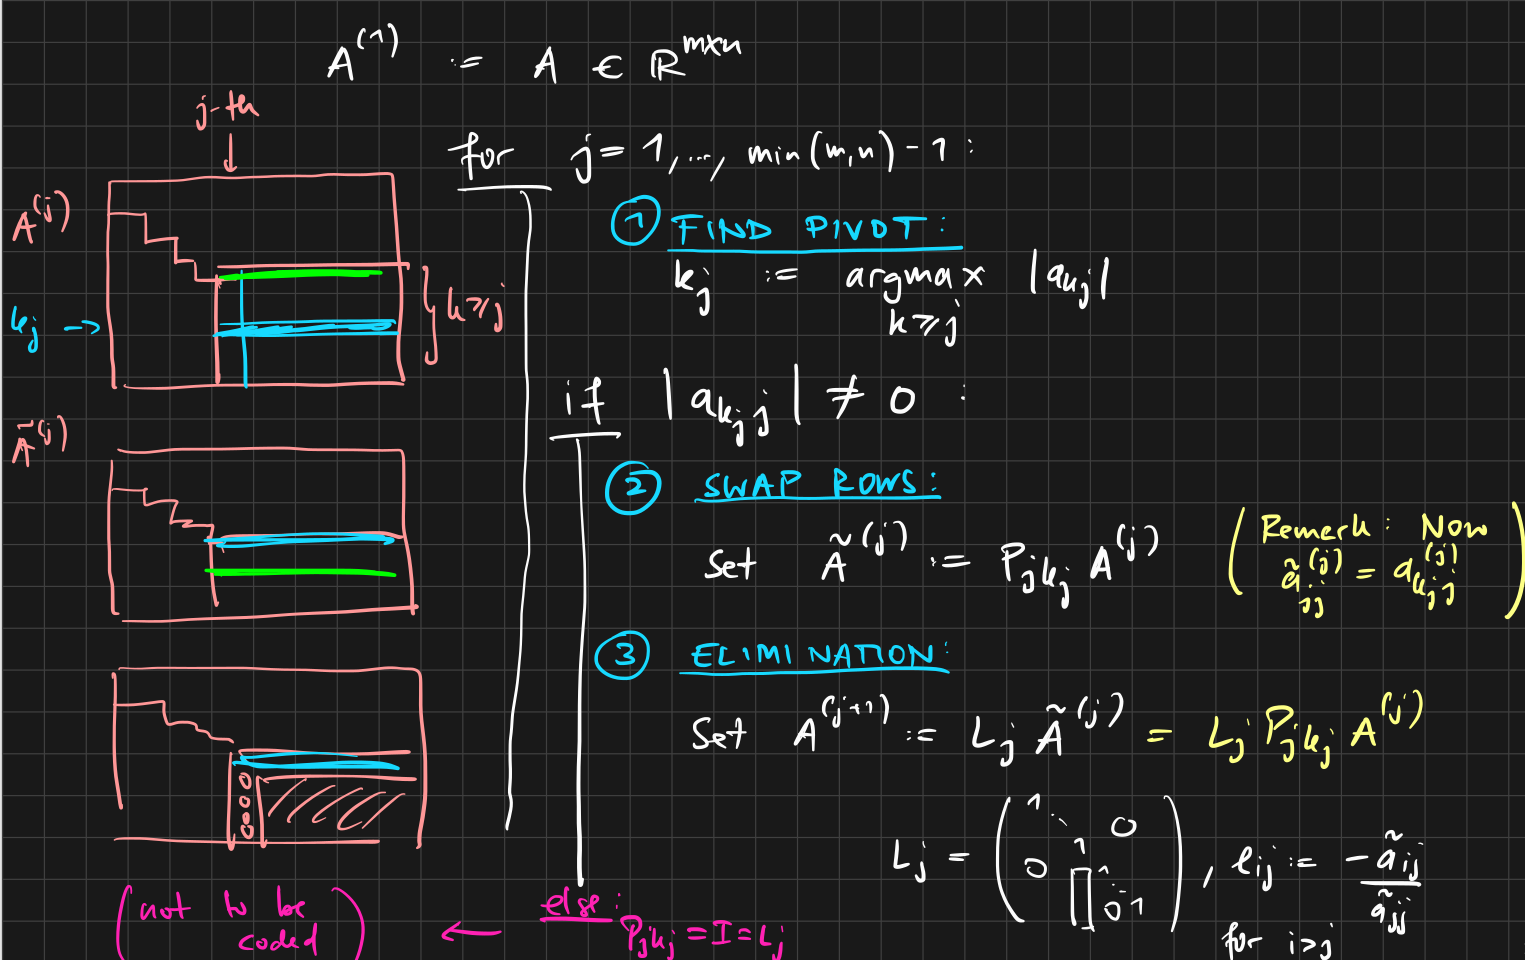
\includegraphics[width=0.9\textwidth]{gaussian-elimination.png}\\~\\~\\	
Remark: We can work \textit{in-place} and store numbers for $L$ and $U$ in the the same array.
		 }
	 
\end{frame}

\begin{frame}

	\textbf{\small In-place Gaussian Elimination with Row Pivoting} (for $m=n$)\\~\\
		\footnotesize
	\textbf{INPUT:} $A\in \mathbb{R}^{n \times n}$ (and $b \in \mathbb{R}^n$)\\
\textbf{OUTPUT:} LU decomposition $PA = LU$ (and if  $Ax = b$ is uniquely solvable the solution $x\in \mathbb{R}^n$)\\
\hspace*{1cm}\begin{algorithm}[H]
		{\color{gray}\texttt{\# \textbf{FACTORIZATION}}}\\
		initialize \texttt{piv = [1,2,...,n]}\\
		\For{$j = 1,...,n-1$}{
			{\color{gray}\texttt{\#  \textbf{Find the j-th pivot}}}\\
			$k_j := \arg \max_{k\geq j} |a_{kj}|$ \label{pivot}\\
			\If{$a_{k_jj}\neq 0$}{
				{\color{gray}\texttt{\# \textbf{Swap rows}}}\\
				A[$k_j$,:] $\leftrightarrow$ A[j,:]\\
				{\color{gray}\texttt{\#  by hand we also transform b on the fly}}\\
				b[$k_j$] $\leftrightarrow$ b[j]\\
				\texttt{piv}[$k_j$] $\leftrightarrow$ \texttt{piv}[j]\\
				{\color{gray}\texttt{\# \textbf{Elimination}}}\\
				\For{$k = j+1,\dots,n$}{
					$\ell_{kj} := a_{kj} / a_{jj}$\\
					$a_{kj} = \ell_{kj}$\\
					
					\For{$i = j+1,\ldots, n$}{
						$a_{ki} = a_{ki} - \ell_{kj} a_{ji}$\\
						
					}
					{\color{gray}\texttt{\#  by hand we also transform b on the fly}}\\
					($b_{k} = b_{k} - \ell_{kj} b_{j}$)
				}
			}
			
		}
		{\color{gray}\texttt{\# \textbf{SOLVE}}}\\
		$\ldots$
	\end{algorithm}
\end{frame}


\color{fontcolor}
\begin{frame}
	~\\
	As in the algorithm consider $A\in\mathbb{R}^{n \times n}$. Then the algorithm eventually leads to
	$$U:=A^{(n)}=L_{(n-1)}P_{(n-1)k_{(n-1)}}\dots L_3P_{3k_3}L_2P_{2k_2}L_1P_{1k_1}A.$$
	~\\
	By construction of the algorithm, $A^{(n)}=:U$ has row echelon form (no rigorous proof provided in this course).
	~\\
~\\
		\textbf{Question:}	Can we group all $L_i$ and $P_{ik_i}$ in such a way that $PA=LU$?\\
		\begin{lemma} \small
			Let $m\in\mathbb{N}$.  Let $P_{ik_i} \in \mathbb{R}^{m \times m}$ be the permutation matrix which results from interchanging the $i$-th and $k_i$-th column of the identity matrix in $\mathbb{R}^{m \times m}$, where $k_i \geq i$. Further for $\ell_j := (0,\ldots,0,\ell_{j+1,j},\ldots,\ell_{m,j})^\top\in\mathbb{R}^m$ and the $j$-th unit vector $e_j\in\mathbb{R}^m$, let $L_j := I + \ell_je_j^\top \in \mathbb{R}^{m\times m}$.
			Then show that for all $1 \leq j< i \leq k_i\leq m$ we have
			$$P_{ik_i} L_j = \widehat{L}_j P_{ik_i}$$
			where $\widehat{L}_j :=  I + (P_{ik_i}\ell_j)e_j^\top$.
		\end{lemma}
	\Hide{	\begin{proof}\small
		 We find
		 \begin{align*}
		 P_{ik_i} L_j
		 &=  P_{ik_i}\left(I + \ell_je_j^\top \right)\\
		 &=  P_{ik_i} +  P_{ik_i}\ell_je_j^\top \\
		 &=  P_{ik_i} +  P_{ik_i}\ell_je_j^\top {\color{cyan}P_{ik_i}^\top P_{ik_i} }\\
		 &= (I +  P_{ik_i}\ell_je_j^\top  P_{ik_i}^\top) P_{ik_i} \\
		 &= (I +  P_{ik_i}\ell_j{\color{cyan} (P_{ik_i}e_j)^\top}) P_{ik_i} .\\
		 &= (I +  P_{ik_i}\ell_j{\color{cyan}e_j^\top}) P_{ik_i} .
		 \end{align*}
		 Since $j~{\color{red}<} ~i \leq k_i$ we find that $P_{ik_i}e_j=e_j$, since only zeroes are swapped.
	\end{proof}
	}
\end{frame}

\begin{frame}
%				We show in the exercise:
%	$$P_{ik_i}L_j=\hat{L}_jP_{ik_i},~~~~1\leq j{\color{cyan}~ <~} i\leq k_i\leq m$$
%\Vspace{3cm}
	By applying this result multiple times, we obtain
\Hide{	\begin{align*}
	\underbrace{(\hat{L}_{n-1}\cdots \hat{L}_{2}\hat{L}_1)}_{=:\widehat{L}}&\underbrace{(P_{(n-1)k_{(n-1)}}\cdots P_{2k_2}P_{1k_1})}_{=:P}\cdot A=U\\
	&\stackrel{L:=\widehat{L}^{-1}}{\Leftrightarrow}~~\\
	&PA=LU.
	\end{align*}}
\end{frame}


\begin{frame}
	Summary: 
	{\bf \large Row echelon form and $LU$ decomposition} ~\\
	\begin{defi}[REF] 
		~\\
		\begin{itemize} 
		\item[a)] \textbf{Row elementary operations} are 
		\begin{itemize}
		\item[1)] add a nonzero multiple of one row to another
		\item[2)] swap two rows
		\end{itemize}
		\item[b)] A matrix is in \textbf{row echelon form (REF)} when it satisfies the following conditions:
		\begin{itemize}
		\item[1)] The first non-zero element in each row (called the leading entry) is in a column to the right of the leading entry in the previous row.
		\item[2)] Rows with all zero elements, if any, are below rows having a non-zero element.
		\end{itemize}
		\end{itemize}
	\end{defi}
	~\\
	By applying these types of operations we find: \vspace{-0.2cm}
	\begin{theo}[LU Decomposition]\label{REF}
		Every matrix $A\in\F^{m\times n}$ can be transformed to REF by row elementary operations. Thus there is a matrix $U\in\F^{m\times n}$ in REF, a lower triangular matrix $L\in GL(m,\F)$ with $\ell_{ij}=0,\forall j>i,$ and $\ell_{ii}=1,\forall i,$ and a permutation matrix $P\in GL(m,\F)$ with exactly one entry ``1'' in each row and column and zero otherwise, such that
		\[
		P\cdot A=L\cdot U.
		\]
	\end{theo}
	~\\
	Since triangular matrices are invertible if and only if the diagonal elements are nonzero, we find for the square case $m=n$, that:\vspace{-0.2cm}
	\begin{corollary}[Invertibility of $A$]\label{corREF}
	A matrix $A\in\F^{n\times n}$ is invertible, if and only if its REF $U\in\F^{n\times n}$ has a nonzero diagonal, i.e, $u_{ii}\neq 0, \forall i=1,\ldots ,n$.
	\end{corollary}
\end{frame}



%%%%%%%%%%%%%%%%%%%%%%%%%%%%%%%%%%%%%%%%%%
% RECAP ON EXAMPLE
%%%%%%%%%%%%%%%%%%%%%%%%%%%%%%%%%%%%%%%%%
%\elomath{
%\begin{frame}
%\textbf{Recap example from above}:\\
%	{\blank
%		 
%		$\textcolor{orange}{ L_2}\underbrace{\textcolor{cyan}{P_{23}}\textcolor{orange}{L_1}}_{=\hat{L}_1P_{23}} \textcolor{cyan}{P_{13}} A = U$\\
%		\underline{j=1:}
%		\begin{align*}
%		\left(
%		\begin{array}{ccc|c}
%		0&2&3&2\\
%		1&3&5&4\\
%		2&4&6&6
%		\end{array}
%		\right)
%		\textcolor{cyan}{
%			\begin{bmatrix}
%			1\\2\\3
%			\end{bmatrix}
%		}
%		\stackrel{\text{I}\leftrightarrow\text{III}}{\rightsquigarrow}
%		\left(
%		\begin{array}{ccc|c}
%		2&4&6&6\\
%		1&3&5&4\\
%		0&2&3&2
%		\end{array}
%		\right)
%		\textcolor{cyan}{
%			\begin{bmatrix}
%			3\\2\\1
%			\end{bmatrix}
%		}
%		&\stackrel{\text{II'=II}-\frac{1}{2}\text{I}}{\rightsquigarrow}
%		\left(
%		\begin{array}{ccc|c}
%		2&4&6&6\\
%		\textcolor{orange}{\frac{1}{2}}&1&2&1\\
%		\textcolor{orange}{0}&2&3&2
%		\end{array}
%		\right)
%		\textcolor{cyan}{
%			\begin{bmatrix}
%			3\\2\\1
%			\end{bmatrix}
%		}\\
%	{\cyan 
%	P_{13}=\begin{pmatrix}
%	0&0&1\\
%	0&1&0\\
%	1&0&0
%	\end{pmatrix}}\hspace{2.5cm}
%&{\red L_1=\begin{pmatrix}
%	1&0&0\\
%	-\frac{1}{2}&1&0\\
%	0&0&1
%	\end{pmatrix}}
%		\end{align*}
%		\underline{j=2:}
%\begin{align*}
%\stackrel{\text{II}\leftrightarrow\text{III}}{\rightsquigarrow}
%\left(
%\begin{array}{ccc|c}
%2&4&6&6\\
%\textcolor{orange}{0}&2&3&2\\
%\textcolor{orange}{\frac{1}{2}}&1&2&1
%\end{array}
%\right)
%\textcolor{cyan}{
%	\begin{bmatrix}
%	3\\1\\2
%	\end{bmatrix}
%}
%&\stackrel{\text{III'=III}-\frac{1}{2}\text{II}}{\rightsquigarrow}
%\left(
%\begin{array}{ccc|c}
%2&4&6&6\\
%\textcolor{orange}{0}&2&3&2\\
%\textcolor{orange}{\frac{1}{2}}&\textcolor{orange}{\frac{1}{2}}&\frac{1}{2}&0
%\end{array}
%\right)
%\textcolor{cyan}{
%	\begin{bmatrix}
%	3\\1\\2
%	\end{bmatrix}
%}
%\begin{matrix}
%\Rightarrow~x_1=1\\
%\Rightarrow~x_2=1\\
%\Rightarrow~x_3=0
%\end{matrix}\\
%{\cyan 
%	P_{23}=\begin{pmatrix}
%	1&0&0\\
%	0&0&1\\
%	0&1&0
%	\end{pmatrix}}\hspace{2.5cm}
%&{\red L_2=\begin{pmatrix}
%	1&0&0\\
%	0&1&0\\
%	0&-\frac{1}{2}&1
%	\end{pmatrix}}
%\end{align*}
%	}
%\end{frame}
%
%\begin{frame}
%	~\\
%	{\blank
%		We find:
%		\begin{align*}
%		&\textcolor{orange}{
%			L=\begin{pmatrix}
%			1&0&0\\
%			0&1&0\\
%			\frac{1}{2}&\frac{1}{2}&1
%			\end{pmatrix}},
%		%
%		U=\begin{pmatrix}
%		2&4&6\\
%		0&2&3\\
%		0&0&\frac{1}{2}
%		\end{pmatrix},
%		%
%		\textcolor{cyan}{
%			P=\begin{pmatrix}
%			0&0&1\\
%			1&0&0\\
%			0&1&0
%			\end{pmatrix}}\\
%		%
%		&\textcolor{orange}{L}U=\begin{pmatrix}
%		1&0&0\\
%		0&1&0\\
%		\frac{1}{2}&\frac{1}{2}&1
%		\end{pmatrix}
%		\begin{pmatrix}
%		2&4&6\\
%		0&2&3\\
%		0&0&\frac{1}{2}
%		\end{pmatrix}
%		=\begin{pmatrix}
%		2&4&6\\
%		0&2&3\\
%		1&3&5
%		\end{pmatrix}\\
%		%
%		&\textcolor{cyan}{P}A=\begin{pmatrix}
%		0&0&1\\
%		1&0&0\\
%		0&1&0
%		\end{pmatrix}
%		\begin{pmatrix}
%		0&2&3\\
%		1&3&5\\
%		2&4&6
%		\end{pmatrix}
%		=\begin{pmatrix}
%		2&4&6\\
%		0&2&3\\
%		1&3&5
%		\end{pmatrix}\\
%		&\Rightarrow~~PA=LU
%		\end{align*}
%	}
%\end{frame}
%%% END ELOMATH
%}



\begin{frame}
%	The so-called ``\textbf{direct}'' (= exact solution in finite steps) solution process for the system $Ax=b$ sketched above comprises two steps:~\\~\\
	\begin{itemize}
		\item[{\bf~(1)}] {\bf~Factorization:}~~~~{\tt Lu, Piv = scipy.linalg.lu\_factor(A)}~\\~\\
		\begin{itemize} \normalsize
			\item determine factors $L,U$ and permutation matrix $P$ such that $LU=PA$\\~\\
			\item the factors $L,U$ are compactly stored in one matrix {\tt Lu} $\in\R^{n\times n}$ of the same size as $A$ and the permutation matrix $P$ in CSR format as integer vector {\tt Piv} $\in\N^{n}$.
		\end{itemize} ~\\
		\vspace{0.8cm}
		\item[{\bf~(2)}] {\bf~Solution:}~~~~~~~~~~~{\tt x = scipy.linalg.lu\_solve((Lu, Piv), b)}~\\~\\
		\begin{itemize}
			\normalsize
			\item[\color{cyan}(2.1)] permute right-hand side $\bar{b}=Pb$~\\~\\
			\item[\color{cyan}(2.2)] solve lower triangular system $Lz=\bar{b}$ for $z$ (forward substitution)~\\~\\
			\item[\color{cyan}(2.3)] solve REF system $Ux=z$ for $x$  (backward substitution)
		\end{itemize}
	\end{itemize}
	~\\
	~\\
	Both, (1) and (2), are combined in the routine $${\tt x = scipy.linalg.solve(A,b)}.$$ 
	%
\end{frame}



 
\begin{frame}
\Subsubsection{Identify the number of solutions from the REF}~\\
%	\textbf{~Identify the number of solutions $|S|$ from the REF $U$}\\
% ~\\~\\
\Hide{ First, by inserting the $LU$ decomposition we obtain
	$$S:=\{x\in\mathbb{R}^n:~Ax=b\}\stackrel{A=P^TLU}{=}\{x\in\mathbb{R}^n:~P^TLUx=b\} = \{x\in\mathbb{R}^n:~Ux=\underbrace{L^{-1}Pb}_{=:z}\}.$$	
	~\\ \small
	Then we find for the three possible cases of the solution set (exercise):
	\begin{itemize}
		\item [1)] $U$ does not have a zero row (i.e., $m\leq n$)
			\begin{itemize}
				\item[1.1)] $m=n$: Then $U$ is invertible and $|S|=1$ with $x=U^{-1}L^{-1}Pb$
				\item[1.2)] $m<n$: Then has dependent columns but $\im(U)=\Rm$, so that $|S|=\infty$\\
				{\footnotesize\color{cyan}Note: The $m$ rows of $U$ are independent. Thus $m = \dim \im U^\top$. Also from dimension formula $ \dim \ker U^\top = m - \dim \im U^\top=0 $, so that $\ker U^\top = \{0\}$ and thus $\im(U) = (\ker U^\top)^\bot = \{0\}^\bot = \Rm$. }¸
			\end{itemize}
%		\item $U$ is invertible ($\Leftrightarrow m=n, ~u_{ii}\neq 0 \forall i$)\\
%		 $\Rightarrow~~|S|=1,~x=U^{-1}L^{-1}Pb$~\\~\\
		\item [2)] $U$ has at least one zero row
					\begin{itemize}
				\item [2.1)]
				For all zero rows in $U$, the transformed right-hand side $z$ is also zero there:\\
				$\Rightarrow~~Ux=z$ has infinitely many solutions, i.e., $|S|=\infty$\\
				~~~~~~(Note: $0x_1+\dots+0x_n=z_i=0$ is true for any $x$)~\\~\\
				\item [2.2)]
				else: $|S|=0$\\
				(Note: $0x_1+\dots+0x_n=z_i\neq0$ false for any $x$)~\\~\\
			\end{itemize}
%		\item $U$ is not invertible:
%		\begin{itemize}
%			\item [2.1)] $m\geq n$ and $U$ has at least one zero row:
%			\begin{itemize}
%				\item [2.1.1)]
%				For all zero rows in $U$, the transformed right-hand side $z$ is also zero there:\\
%				$\Rightarrow~~Ux=z$ has infinitely many solutions, i.e., $|S|=\infty$\\
%				~~~~~~(Note: $0x_1+\dots+0x_n=z_i=0$ is true for any $x$)~\\~\\
%				\item [2.2.2)]
%				else: $|S|=0$\\
%				(Note: $0x_1+\dots+0x_n=z_i\neq0$ true for no $x$)~\\~\\
%			\end{itemize}
%		  \item [2.2)] $m< n$: exercise?
%		\end{itemize}
	\end{itemize}
}
\end{frame}
 
 
%%%%%%%%%%%%%%%%%%%%%%%%%%%%%%%%%%%%%%%%%%
% ELOMATH: MORE ON LU
%%%%%%%%%%%%%%%%%%%%%%%%%%%%%%%%%%%%%%%%%
%\elomath{
%%%%%%%%%%%%%%%%%%%%%%%%%%%%%%%%%%%%%%%%%
% The Rank of $A$ from $U$
%%%%%%%%%%%%%%%%%%%%%%%%%%%%%%%%%%%%%%%%
%\begin{frame}
% \textbf{~The Rank of $A$ from $U$}\\
% 	\centering
% 	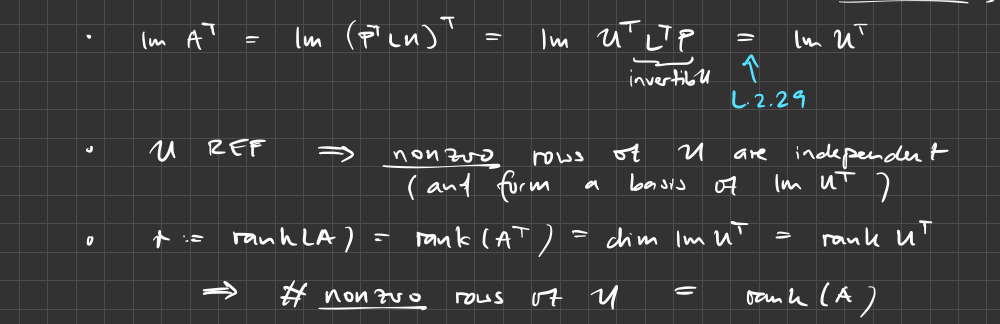
\includegraphics[width=0.9\linewidth]{lu-rank}
%\end{frame} 
% 


%%%%%%%%%%%%%%%%%%%%%%%%%%%%%%%%%%%%%%%%%
% Block Elimination and the Schur Complement
%%%%%%%%%%%%%%%%%%%%%%%%%%%%%%%%%%%%%%%%
%\begin{frame}
%	\Subsubsection{Block Elimination and the Schur Complement}
%		\centering
%		\Hide{\includegraphics[width=0.9\linewidth]{lu-block1}}
%\end{frame}  
%\begin{frame}
%%	\textbf{~Block Elimination and the Schur Complement}\\
%		\centering
%		\Hide{\includegraphics[width=0.9\linewidth]{lu-block2}}
%\end{frame}  
%\begin{frame}
%%	\textbf{~Block Elimination and the Schur Complement}\\
%	\centering
%		\Hide{\includegraphics[width=0.9\linewidth]{lu-block3}}
%\end{frame}  
%\begin{frame}
%%	\textbf{~Block Elimination and the Schur Complement}\\
%		\centering
%		\Hide{\includegraphics[width=0.9\linewidth]{lu-block4}}
%\end{frame}  


%%%%%%%%%%%%%%%%%%%%%%%%%%%%%%%%%%%%%%%%%
% Understanding Elimination as Substracting Rank-1 Pieces
%%%%%%%%%%%%%%%%%%%%%%%%%%%%%%%%%%%%%%%%
%\begin{frame}
%	\textbf{~Understanding Elimination as Substracting Rank-1 Pieces}\\
%		\centering
%	\includegraphics[width=0.95\linewidth]{lu-understanding-as-subs-rank1_1}
%\end{frame}  
%\begin{frame}
%	\centering
%	\includegraphics[width=0.95\linewidth]{lu-understanding-as-subs-rank1_2}
%\end{frame}  


%%%%%%%%%%%%%%%%%%%%%%%%%%%%%%%%%%%%%%%%%
% ROUNDING ERRORS
%%%%%%%%%%%%%%%%%%%%%%%%%%%%%%%%%%%%%%%%	
%\begin{frame}
%\Subsubsection{Pivoting to reduce rounding errors}	
%\Hide{
%	\begin{itemize}
%		\item In the above factorization procedure we went from column to column and eliminated the values under the diagonal element (the \textit{pivot element}). \vspace{0.2cm}
%		\item In order to reduce rounding errors one chooses the element in the current column which has largest absolute value as the pivot element (by permuting rows first).
%	\end{itemize}
%}
%\end{frame}
%\begin{frame}
%		~\\
%		\Hide{
%			\textbf{~Example} (rounding errors)\\
%			Let $\varepsilon\ll 1$ small enough, such that with machine precision
%			$$
%			{\yellow 1\pm \varepsilon =1}
%			$$
%			Consider
%			$$
%			A=\begin{pmatrix}
%			\varepsilon&2\\1&1
%			\end{pmatrix},
%			~b=\begin{pmatrix}
%			1\\1
%			\end{pmatrix}
%			~~\Rightarrow~~x_1=\frac{1}{2-\varepsilon}\approx\frac{1}{2},
%			~x_2=\frac{1-\varepsilon}{2-\varepsilon}\approx\frac{1}{2}
%			$$
%			Solve with elimination:\begin{itemize}
%				\item [1)]
%				\underline{No pivoting:}
%				\begin{align*}
%				&\left(
%				\begin{array}{cc|c}
%				\varepsilon&2&1\\
%				1&1&1
%				\end{array}
%				\right)
%				\stackrel{\text{II'=II}-\frac{1}{\varepsilon}\text{I}}{\rightsquigarrow}
%				\left(
%				\begin{array}{cc|c}
%				\varepsilon&2&1\\
%				0&1-\frac{2}{\varepsilon}&1-\frac{1}{\varepsilon}
%				\end{array}
%				\right)\\
%				\Rightarrow~~&x_2=\frac{1-\frac{1}{\varepsilon}}{1-\frac{2}{\varepsilon}}
%				=\frac{\varepsilon}{\varepsilon}\frac{1-\frac{1}{\varepsilon}}{1-\frac{2}{\varepsilon}}=\frac{\varepsilon-1}{\varepsilon-2}{\cyan\cong}\frac{1}{2}~~{\cyan(\text{machine precision})}\\
%				\Rightarrow~~&\varepsilon x_1+2\frac{1}{2}=1~~\Leftrightarrow~~x_1{\cyan\cong}0~~{\cyan(\text{machine precision})}
%				\end{align*}
%				\item [2)]
%				\underline{Pivoting:}
%				\begin{align*}
%				&\left(
%				\begin{array}{cc|c}
%				\varepsilon&2&1\\
%				1&1&1
%				\end{array}
%				\right)
%				\stackrel{\text{I}\leftrightarrow\text{III}}{\rightsquigarrow}
%				\left(
%				\begin{array}{cc|c}
%				1&1&1\\
%				\varepsilon&2&1
%				\end{array}
%				\right)
%				\stackrel{\text{II'=II}-\varepsilon\text{I}}{\rightsquigarrow}
%				\left(
%				\begin{array}{cc|c}
%				1&1&1\\
%				0&2-\varepsilon&1-\varepsilon
%				\end{array}
%				\right)\\
%				\Rightarrow~~&x_2=\frac{1-\varepsilon}{2-\varepsilon}{\cyan\cong}\frac{1}{2}~~{\cyan(\text{machine precision})}\\
%				\Rightarrow~~&x_1=1-x_2=\frac{1}{2}~~{\green\checkmark~\text{much better approximation}}
%				\end{align*}
%			\end{itemize}
%		}
%	\end{frame}	
%}




%%%%%%%%%%%%%%%%%%%%%%%%%%%%%%%%%%%%%%%%%
% CHOLESKY
%%%%%%%%%%%%%%%%%%%%%%%%%%%%%%%%%%%%%%%%
\begin{frame}[c]
	\hspace*{1.5cm}		\Subsection{The Cholesky Decomposition}
\end{frame}
	
\begin{frame}
	For symmetric and positive definite matrices $A\in \Rnn_{\text{spd}}\subset \text{GL}_n(\R)$ we obtain the following improvement:
	\begin{theorem}
		We have the equivalence
		$$A\in \Rnn_{\text{spd}} ~~\Leftrightarrow~~\exists_1~ L \in \Rnn \text{\emph{lower triangular}},~\ell_{ii}>0\colon~~ A = LL^\top.$$
	\end{theorem}
%	$$A=LL^T$$
%	for $L\in\Rnn$ being a lower triangular matrix (i.e., $U = L^\top$).
%	
~\\~\\
\begin{itemize}
	\item The Decomposition $A = LL^\top$ is called the \textbf{\color{defgruen} Cholesky decomposition of $A$}.
	\item Named after the french Mathematician André-Louis Cholesky (1875-1918) who developed this decomposition during his surveying work to solve the normal equation $A^\top A x = A^\top b$.
	\item We can derive an algorithm to compute the factor $L$.
	~\\~\\
	\item \textbf{Solving using $A=LL^\top$}\\
	$$Ax = b ~~\Leftrightarrow~~ LL^\top x = b ~~\Leftrightarrow~~ Lz = b,~~L^\top x = z~~~(\text{forward/backward Subst.})$$
\end{itemize}	
~\\~\\~\\
	\textit{In Python:}
	\begin{itemize}
		\item[{\bf~(1)}] {\bf~Factorization:}~~~~{\tt L, lower = scipy.linalg.cho\_factor(A)}~\\~\\
		\vspace{0.2cm}
		\item[{\bf~(2)}] {\bf~Solution:}~~~~~~~~~~~{\tt x = scipy.linalg.cho\_solve((L, lower), b)}
	\end{itemize}
\end{frame}
 
 
%%%%
% ELOMATH: More Remarks on Cholesky
%%%% 
%\elomath{
%\begin{frame}
%For the remainder, $A$ is assumed to be symmetric and positive definite.
%~\\~\\
%\textbf{~Remarks}
%\begin{itemize}
%	\item For $A \in \Rnn_{\text{spd}}$ we have $a_{ii} > 0$ (positive diagonal entries):\\
%	\Hide{~\\
%	For the unit vector $e_i$ we have $$a_{ii} = e_i^\top A e_i > 0. $$
%	~\\
%}
%\item \textbf{The $LDL$ Decomposition}\\~\\
%	\includegraphics[width=0.9\linewidth]{cholesky-ldl}
%\end{itemize}
%\end{frame}
%\begin{frame}
%	\begin{itemize}
%		\item \textbf{The Determinant of $A$}\\~\\
%			\includegraphics[width=0.99\linewidth]{cholesky-determinant}	
%	\end{itemize}
%\end{frame}
%\begin{frame}
%	\Subsubsection{Computation: ``Column by Column''}
%	By the theorem above we know that there exists an unique lower triangular matrix $L$ with positive diagonal entries $\ell_{ii} > 0$, so that
%	$$A= LL^\top.$$ 
%	By comparing each entry we obtain 
%	\Hide{~\\
%	\begin{align*}
%	a_{ik} = (LL^\top)_{ik} = \sum_{j=1}^n \ell_{ij}\underbrace{\widetilde{\ell}_{jk}}_{=\ell_{kj}} = \sum_{j=1}^n \ell_{ij}\underbrace{\ell_{kj}}_{=0,~k<j} = \sum_{j=1}^k\ell_{ij}\ell_{kj}
%	\end{align*}
%	~\\~\\~\\
%}	
%	From here we can now derive formulas for the entries $\ell_{ik}$ of $L$ which allow us to compute the matrix $L$ column by column.\\~\\ More precisely, for the $k$-th column of $L$ we obtain
%	\begin{itemize}
%		\item Above diagonal: $i<k$ ~\\
%		$$\ell_{ik} = 0 $$
%	\end{itemize}
%\end{frame}
%
%\begin{frame}
%	\Hide{~\\
%\begin{itemize}
%	\item Diagonal element: $i=k$
%    \item Below diagonal: $i>k$
%\end{itemize}
%\includegraphics[width=0.99\linewidth]{cholesky-computation}
%~\\
%}
%\end{frame}
%
%\begin{frame}
%\textbf{~Remarks}\\~\\
%\begin{itemize}
%	\item The algorithm can work \textbf{in-place}: Once the data of a column of $A$ was accessed, it is no more needed in subsequent calculations.\\~\\
%	\item If, despite the symmetry of $A$, also the upper triangular part of $A$ was stored, then clearly this part needs to be zeroed at the end of the in-place algorithm.\\~\\
%	\item Using the algorithm as \textbf{test for the spd--property}:\\
%	The theorem tells us that $\ell_{ii}>0$; the algorithm computes $\ell_{ii}$. Thus, if we apply the algorithm to a matrix $A \in \Rnn$ and along the way we obtain $\ell_{ii} \leq 0$, then we know that the matrix is \textbf{not} positive definite.
%\end{itemize}	
%\end{frame}
%
%\begin{frame}
%	\Subsubsection{Comparison to Gaussian Elimination}
%	~\\
%	First note that 
%	$$A=LL^\top ~~\Leftrightarrow~~L^{-1} A = L^\top =~\text{upper triangular} $$
%	~\\
%	\begin{itemize}
%		\item $L^{-1}$ contains the ``elimination steps'' that transform $A$ into an upper triangular system.
%		\item However, here we can use a different approach to find the factors: Instead of applying row elementary operations we are able to derive closed formulas for $L$ directly from $A = LL^\top$ (since ``$U=L^\top$'').
%	\end{itemize}
%	~\\~\\
%	\textbf{Gaussian Elimination applied to a spd-Matrix}\\~\\
%	{\color{satzrot}\textbf{One can show:} For a symmetric and positive definite matrix $A$ there is no row pivoting needed (other than for stability reasons), i.e., there exist triangular matrices $L$ (lower) with 1's on the diagonal and $U$ (upper) so that $$A = LU.$$ }
%	\textbf{Question:} Is this the Cholesky decomposition? The answer is ``no'', which we will see in the example below.
%\end{frame}
% \begin{frame}
% 	\textbf{Example}\\~\\
% 	\includegraphics[width=0.99\linewidth]{cholesky-example}
% \end{frame}
%}

\begin{frame}
	\textbf{~Numerical Comparison: LU vs. Choleskly}\\~\\
	\begin{itemize}
		\item \textbf{Computational Costs:} ~\\The Cholesky decomposition is roughly twice as fast as Gaussian elimination (in terms of number of floating point operations). Clearly, we only need to compute one instead of two factors.\\~\\
		\item \textbf{Stability} (=``robustness against rounding errors'') :
		\begin{itemize}\normalsize
			\item Gaussian Elimination: Is only stable if a pivoting strategy is applied.
			\item Cholesky: Is stable even without pivoting.\\ (To avoid square roots, one can compute the LDL decomposition)
		\end{itemize}
	\end{itemize}
~\\~\\
\textbf{All in all:} \begin{center}
	\textit{For symmetric and positive definite matrices (of moderate size),\\ the Cholesky factorization is the preferred algorithm!}
\end{center}
\end{frame}




% eigvals
\only<presentation>{\setnextsection{3}}
\lecture{Eigenvalues: Theory and Algorithms}{eigvals}
% !TeX spellcheck = en_US
\color{fontcolor}

\begin{frame}
	Recommended reading:
	\begin{itemize}
		\item Lectures 24, 25, 27 in \cite{TreBau}
		\item Sections I.6 in \cite{StrangData}
		\item Sections 6.1, 6.2, 6.4 in \cite{StrangLA_intro}	
		\item Kapitel 7 in \cite{Rannacher}
	\end{itemize}
	
	%	\bibliographystyle{plain}
	~\\~\\
	Literature:\\
	\bibliography{../information/literature.bib}
\end{frame}
\begin{frame}
\Section{Eigenvalues: Theory and Algorithms}	
\Subsection{Introduction}
\Hide{
\begin{example}[Illustration in 2d: Part 1]\label{ex:eigvals-Illustration-2d-1}
	~\\
		\includegraphics[width=0.94\textwidth]{eigenvalues_example.png}
\end{example}
}
\end{frame}




% EIGENVALUES
\begin{frame}
\Subsection{Eigenvalues and Eigendecompositon}
\begin{defi}[Eigenvalues and -vectors]\label{def:eigvals}
	Let $A\in\F^{n\times n}$ be a matrix. A number $\lambda\in \C$ is called an \textbf{\emph{eigenvalue}} of $A$, if 
	$$\exists v\in \F^n, v\neq 0\colon~Av=\lambda v.$$ In that case, $v$ is called an \textbf{\emph{eigenvector}} and $(\lambda, v)$ an \textbf{\textit{eigenpair}}. The set of all eigenvalues is denoted by
	$$\sigma(A):=\{\lambda\in \C\colon \lambda \text{ is eigenvalue of }A\}$$ and called the \textbf{\emph{spectrum of $A$}}.
\end{defi}

\begin{itemize}
	\item[1)] Assume we knew an eigenvalue $\lambda$:\\
		\Hide{
	Then we find a corresponding eigenvector by solving the linear equation $$(A - \lambda I_n)v = 0 $$
	Observation: 
	\begin{center}
		$v$ eigenvector ~~~$\Rightarrow$~~~ $\alpha v$ eigenvector $\forall \alpha\in \F$
	\end{center}

~\\
	 We often normalize the eigenvector by $\frac{v}{\|v\|_2}$. } 
    \vspace{0.5cm}
	\item[2)]  Assume we had an eigenvector $v$:\\
		\Hide{
		Then the corresponding eigenvalue is uniquely determined by the so-called \textit{Rayleigh-Quotient} $$ \lambda =  \frac{v^TAv}{v^Tv}$$}
\end{itemize}
\end{frame}



% DETERMINANTS AND EIGENVALUES
\begin{frame}
\textbf{The determinant and eigenvalues}\\~\\
Let $A\in \F^{n \times n}$. Then:~\\
\Hide{
\begin{itemize}
	\item[1)] \textbf{Relation between the determinant and eigenvalues:}
	\begin{align*}
	\lambda\in\C \text{~eigenvalue of~} A ~~& \Leftrightarrow~~\exists v\neq 0\colon Av = \lambda v    ~~\Leftrightarrow ~~\exists v\neq 0\colon~(A-\lambda I_n)v = 0 \\[0.25cm]
	~~& \Leftrightarrow~~\exists v\neq 0\colon~v \in \ker(A-\lambda I_n)  ~~ \Leftrightarrow~~ (A-\lambda I_n) \text{~not injective} \\[0.25cm]
	~~& \Leftrightarrow~~ (A-\lambda I_n) \notin \text{GL}(n,\mathbb{F}) ~~\Leftrightarrow ~~\det (A-\lambda I_n) =0
	\end{align*}
	\item[2)] \textbf{Implication:}\\
	By invoking the Laplace formula (see Def.\ref{def:Laplace-formula}) for the determinant we can show that the function $$\lambda \mapsto \chi_A(\lambda) := \det (A-\lambda I_n)$$ is a \textbf{polynomial of degree} $\leq n$. Thus, we can state:
	$$\textit{\textbf{ The eigenvalues of $A$ are the roots of the polynomial $\chi_A(\lambda)$}}.$$
	The fundamental theorem of algebra then assures the existence of eigenvalues (at most $n$ distinct ones).~\\
	~\\
	Definition: The polynomial $\chi_A(\lambda)$ is called \textbf{\color{defgruen}characteristic polynomial of $A$}.
\end{itemize}
}
\end{frame}


% ILLUSTRATION in 2d
\begin{frame}
\Hide{
\begin{example}[Illustration in 2d: Part 2] \label{ex:eigvals-Illustration-2d-2}~\\
	Let us consider the $(2\times 2)$ matrix 
	$$
	A = \begin{pmatrix}
	2&1\\1&2
	\end{pmatrix}
	$$
	from Example \ref{ex:eigvals-Illustration-2d-1} above.
	
	\begin{itemize}
		\item We compute its eigenvalues by solving the following root finding problem:
			\begin{align*}
		&0=\chi_A(\lambda)=\text{det}(A-\lambda I)=~\text{det}\left(\begin{pmatrix}
		2-\lambda&1\\1&2-\lambda
		\end{pmatrix}\right) = (2-\lambda)^2-1\\
		&\Leftrightarrow~~\lambda\in\{3,1\}=:\{\lambda_1,\lambda_2\}=\sigma(A)
		\end{align*}
		\item Now that we have the eigenvalues we can find corresponding eigenvectors by solving the following homogeneous linear systems:\\
\begin{itemize}
	\item 		For $\lambda_1 = 3$:
		
		$$(A-\lambda_1 I)v^1=0~~\Leftrightarrow~~\begin{pmatrix}
		-1&1\\1&-1
		\end{pmatrix}v^1=0~~\Rightarrow~~v_1^1-v_2^1=0$$
		Thus, the set of all eigenvectors corresponding to the eigenvalue $\lambda_1$ is given by
	$$
		E(\lambda_1):=\{v\in\mathbb{R}^2:~Av=\lambda_1v\}~~=~~\{v\in\mathbb{R}^2:~v_1^1=v_2^1\}
		=~~\lbrace\begin{pmatrix}\alpha\\
		\alpha\end{pmatrix}\in\mathbb{R}^2:~\alpha\in\mathbb{R}\rbrace
		=~~\text{span}\left(\begin{pmatrix}1\\1\end{pmatrix}\right)
		$$
		~\\
		Sometimes it is reasonable to choose eigenvectors of length $1$, so that we normalize: $v^1 = \frac{1}{\sqrt{2}} \begin{pmatrix}1\\1\end{pmatrix}$\\~\\
\end{itemize}
	\end{itemize}


\end{example}
}
\end{frame}

\begin{frame}
	~\\
\Hide{	\begin{itemize}
		\item[] \begin{itemize}
			\item 	For $\lambda_2 = 1$:
	$$
	(A-\lambda_2 I)v^2=0~~\Leftrightarrow~~\begin{pmatrix}
	1&1\\1&1
	\end{pmatrix}v^2=0~~\Leftrightarrow~~v_1^2+v_2^2=0
	$$
	Thus, the set of all eigenvectors corresponding to the eigenvalue $\lambda_2$ is given by
	$$	
	E(\lambda_2) 
	:= \{v\in\mathbb{R}^2:~Av=\lambda_2v\}
	=\{v\in\mathbb{R}^2:~v_1^2=-v_2^2\}
	=\lbrace\begin{pmatrix} \alpha\\-\alpha\end{pmatrix}\in\mathbb{R}^2:~\alpha\in\mathbb{R}\rbrace
	=\text{span}\left(\begin{pmatrix}1\\-1\end{pmatrix}\right) $$
	~\\
	Normalization: Choose $v^2 = \frac{1}{\sqrt{2}} \begin{pmatrix}1\\-1\end{pmatrix}$\
		\end{itemize}
	\item[] ~\\~\\
	\textit{Remark:}\\ The set of all eigenvectors corresponding to the eigenvalue $\lambda \in \sigma(A)$, i.e., $$E(\lambda) = \ker(A-\lambda I) \subset \F^n$$  is called \textbf{\color{defgruen}eigenspace to the eigenvalue $\lambda$ of $A$}.
	\end{itemize}
}
\end{frame}



\begin{frame}
\begin{lemma}[Matrix and Eigenvalue Properties]\label{lem:properties_eigenvalues}~\\[-0.1cm]
	\begin{itemize}
	\item[\color{satzrot}i)]Power of a matrix: $A \in \F^{n\times n} ,~\lambda \in \sigma(A) ~~\Rightarrow~~  \lambda^k \in \sigma(A^k)~\text{for any}~k\in \N$ 
	\vspace{0.2cm}\item[\color{satzrot}ii)] Inverse matrix: $A \in GL_n(\F),~\lambda \in \sigma(A) ~~\Rightarrow~~ \lambda\neq 0,~\frac{1}{\lambda} \in \sigma(A^{-1})~$
	\vspace{0.2cm}\item[\color{satzrot}iii)]Scaling: $A \in \Fnn,~\lambda \in \sigma(A)~~\Rightarrow~~\alpha \lambda \in \sigma(\alpha A) ~~\text{for any} ~\alpha \in \F$
	\vspace{0.2cm}\item[\color{satzrot}iv)] $A \in \F^{n\times n}$hermitian $(A = A^H)$ $~~\Rightarrow~~ \sigma(A)\subset\R$.
	\vspace{0.2cm}\item[\color{satzrot}v)]  $Q \in \Fnn$ unitary ($Q^HQ=I$), $\lambda \in \sigma(Q) ~~\Rightarrow~~|\lambda|=1$
	\vspace{0.2cm}\item[\color{satzrot}vi)] $A \in \F^{n\times n}$ positive definite (semi-definite) ($x^HAx>0$ ($\geq 0$)) $~~\Leftrightarrow~~\forall \lambda \in \sigma(A)\colon~ \lambda > 0~  (\lambda \geq 0)$
	\vspace{0.2cm}\item[\color{satzrot}vii)] The eigenvalues of an upper (lower) triangular matrix are sitting on the diagonal.
	\vspace{0.2cm}\item[\color{satzrot}viii)] Similarity transformation: $A \in \Fnn, ~T \in GL_n(\F) ~~\Rightarrow~~ \sigma(A) = \sigma(T^{-1}AT)$
	\vspace{0.2cm}\item[\color{satzrot}ix)] Shifts: $A \in \Fnn,~ (\lambda, v)$ eigenpair of $A  ~~\Rightarrow~~ \forall s\in\F \colon ~ (\lambda+s, v)$ eigenpair of $A+sI$	
\end{itemize}
\end{lemma}


~\\~\\
\textbf{Attention:} The following rules do not hold in general:\\[-0.1cm]
\begin{itemize}
	\item $\lambda \in \sigma(A), \mu \in \sigma(B)~~~\nRightarrow~~~(\lambda + \mu) \in \sigma(A+B)$
	\item $\lambda \in \sigma(A), \mu \in \sigma(B)~~~\nRightarrow~~~(\lambda \cdot \mu) \in \sigma(A\cdot B)$
\end{itemize}
\end{frame}


\begin{frame}
	\begin{proof}
		Exercise. \Hide{Here, we exemplary prove viii):
		}
	\end{proof}
\end{frame}






%DIAGONALIZING
\begin{frame}
\textbf{Diagonalizing a matrix}\\
\Hide{
	~\\
Let us consider a matrix
$A\in\mathbb{F}^{n\times n}$ with eigenpairs $(\lambda_i,v_i)\in\F \times\mathbb{F}^n$, so that 
$$Av_i = \lambda_i v_i,~~~\text{for}~1\leq i\leq n.$$ 
Using matrix notation this can be written as
\begin{align*}
A\cdot\underbrace{\begin{pmatrix}
|&|&~&|\\v_1&v_2&\cdots&v_n\\|&|&~&|
\end{pmatrix}}_{=:V\in\mathbb{F}^{n\times n}}
&=\begin{pmatrix}
|&|&~&|\\\lambda_1 v_1&\lambda_2 v_2&\cdots&\lambda_n v_n\\|&|&~&|
\end{pmatrix}
=\begin{pmatrix}
|&~&|\\v_1&\cdots&v_n\\|&~&|
\end{pmatrix}
\underbrace{\begin{pmatrix}
\lambda_1&~&0\\~&\ddots&~\\0&~&\lambda_n
\end{pmatrix}}_{=:\Lambda\in\mathbb{F}^{n\times n}}
\end{align*}
which is equivalent to
$$A V = V \Lambda .$$
~\\
If $V$ is invertible (note that this is not necessarily the case!), then we can rearrange this into the following decomposition
$$
V^{-1}AV=\Lambda~~\Leftrightarrow~~A=V\Lambda V^{-1}.
$$
~\\
One central question arises:  When is $V$ invertible?
}
\end{frame}

\begin{frame}
Let us first revisit the example from above (see Examples \ref{ex:eigvals-Illustration-2d-1} and \ref{ex:eigvals-Illustration-2d-2})\\~\\
\Hide{~\\
\begin{example}[Illustration in 2d: Part 3] \label{ex:eigvals-Illustration-2d-3}~\\
Let us again consider the \textit{real symmetric} matrix
$$A=\begin{pmatrix}
2&1\\1&2
\end{pmatrix},$$
with eigenpairs
$$\lambda_1=3,~v_1=\frac{1}{\sqrt{2}}\begin{pmatrix}1\\1\end{pmatrix},~~~~
\lambda_2=1,~v_2=\frac{1}{\sqrt{2}}\begin{pmatrix}1\\-1\end{pmatrix}.$$
~\\
Assembling the normalized eigenvectors into the matrix $V$ yields
$$
V=\frac{1}{\sqrt{2}}
\begin{pmatrix}
1&1\\1&-1
\end{pmatrix}.$$
~\\
Since for the columns we have
\begin{align*}
~\begin{pmatrix}1\\1\end{pmatrix}^T\begin{pmatrix}1\\-1\end{pmatrix}=1-1=0
\end{align*}
and by construction
$$
\|v_1\|_2=\frac{1}{\sqrt{2}}\underbrace{\lVert\begin{pmatrix}1\\1\end{pmatrix}\rVert}_{=\sqrt{2}}=1,~~~\text{and similarly}~~ \|v_2\|_2 = 1,
$$
we find that $V$ is orthogonal and thus in particular invertible.
\end{example}
}
\end{frame}



% EXAMPLE
\only<article>{
\begin{ex}
	 
	Symmetric matrix: $A = \begin{bmatrix}
	4 & 2 \\
	2 & 1
	\end{bmatrix}$\\
	\begin{align*}
	p(\lambda) &= \alpha_0 + \alpha_1\lambda + \alpha_2 \lambda^2 = 2-2\lambda + \lambda^2\\
	&= (4\cdot 1-2\cdot 2)-(4+1)\lambda +\lambda^2 \\
	&=-5\lambda + \lambda ^2 \\
	&=(-5+\lambda)\lambda \\
	&\Rightarrow \lambda_1 = 0, \lambda_2 = 5 \;\;\text{(eigenvalues)}\\
	\end{align*}
	eigenvectors:
	\begin{itemize} 
		\item[$v1$)] \begin{align*}
		&Av=\lambda v \Leftrightarrow (A-\lambda I)v=0\\[10pt]
		&\begin{bmatrix}
		4 & 2 \\
		2 & 1
		\end{bmatrix} \begin{bmatrix}
		x_1 \\
		x_2
		\end{bmatrix} = \begin{bmatrix}
		0 \\
		0
		\end{bmatrix} \underrightarrow{REF} \begin{bmatrix}
		4 & 2 \\
		0 & 0
		\end{bmatrix} \begin{bmatrix}
		x_1 \\
		x_2
		\end{bmatrix} = \begin{bmatrix}
		0 \\
		0
		\end{bmatrix}\\[10pt]
		&4x_1 + 2x_2 = 0 \Rightarrow 2x_1 + x_2 =0 \Rightarrow x_2=-2x_1\\[10pt]
		&v_1 = r \left( \begin{array}{c}
		1 \\
		-2 
		\end{array} \right), r\in \mathbb{R} \;\; \text{normed eigv:~} \overline{v_1} = \frac{1}{\sqrt{5}}\left(\begin{array}{c}
		1 \\
		-2 
		\end{array} \right)
		\end{align*}\\
		\item[$v2$)] \begin{align*}
		&A - \lambda_2 I = \begin{bmatrix}
		4 & 2 \\
		2 & 1
		\end{bmatrix} - 5\begin{bmatrix}
		1 & 0 \\
		0 & 1
		\end{bmatrix} = \begin{bmatrix}
		-1 & 2 \\
		2 & -4
		\end{bmatrix}\\
		&\begin{bmatrix}
		-1 & 2 \\
		2 & -4
		\end{bmatrix}\begin{bmatrix}
		x_1 \\
		x_2
		\end{bmatrix} = \begin{bmatrix}
		0 \\
		0
		\end{bmatrix} \Rightarrow (REF) \begin{bmatrix}
		-1 & 2 \\
		0 & 0
		\end{bmatrix} \begin{bmatrix}
		x_1 \\
		x_2
		\end{bmatrix} = \begin{bmatrix}
		0 \\
		0
		\end{bmatrix}\\
		&\Rightarrow x_1 = 2x_2 \;\;\Rightarrow\;\; v_2 = r \left( \begin{array}{c}
		2 \\
		1
		\end{array} \right) \Rightarrow \bar{v_2} = \frac{1}{\sqrt{5}}\left(\begin{array}{c}
		2 \\
		1 
		\end{array} \right)
		\end{align*}
	\end{itemize}	
	Test that they are orthogonal:\\
	\begin{align*}
	M &:= [\bar{v_1},\bar{v_2}] = \frac{1}{\sqrt{5}} \begin{bmatrix}
	1 & 2 \\
	-2 & 1
	\end{bmatrix} \;\; \text{is orthogonal} \\
	M^\top M &= \frac{1}{\sqrt{5}} \begin{bmatrix}
	1 & -2 \\
	2 & 1
	\end{bmatrix}, \frac{1}{\sqrt{5}} \begin{bmatrix}
	1 & 2 \\
	-2 & 1
	\end{bmatrix} = \frac{1}{\sqrt{5}} \begin{bmatrix}
	1 & -2 \\
	2 & 1
	\end{bmatrix} \begin{bmatrix}
	1 & 2 \\
	-2 & 1
	\end{bmatrix} = \begin{bmatrix}
	1 & 0 \\
	0 & 1
	\end{bmatrix}
	\end{align*}
\end{ex}
}






%%%%%%%%%%%%%%%%%%%%%%%%%%%%%%%%%%%%%%%%%%%%%%%%%%%%%%%%%%%
% PYTHON EXAMPLE with heat equation
\only<article>{
\begin{minipage}[c]{0.35\textwidth}
	{\bf Eigenvalues of the symmetric \\
		matrix:}
	
	\medskip
	{\small
		$A=
		-\begin{pmatrix} 
		-2F & F\\
		F & -2F & F \\
		& \ddots & \ddots & \ddots\\
		&        &  F     & -2F    
		\end{pmatrix}
		$
	}
	
	for varying grid sizes ordered in size. $x$-axis is just the current number of the ordered eigenvalues, i.e., the bullet points are the
	pairs $(\frac{i}{\tt Nx}, \lambda_i)$.
	
	\begin{tikzpicture}
	\node[inner sep=0pt] (dina0) at (0,0)
	{\includegraphics[width=\textwidth]{LocalFolder/LocalMedia/5_heat1D-eigs.png}};
	\end{tikzpicture}
	
\end{minipage}
\begin{minipage}[c]{0.05\textwidth}
	\
\end{minipage}
\begin{minipage}[c]{0.6\textwidth}
%	\lstinputlisting{LocalFolder/LocalMedia/python_examples/5_heat1D-eig.py}
\end{minipage}
%%%%%
\begin{minipage}[c]{0.4\textwidth}
	{\bf Selected eigenvectors:}
	
	\begin{tikzpicture}
	\node[inner sep=0pt] (dina0) at (0,0)
	{\includegraphics[width=\textwidth]{LocalFolder/LocalMedia/5_eigv_30.png}};
	\end{tikzpicture}
	(Note: ``frequency$_i$''$=\sqrt{\lambda_i}$)
\end{minipage}
\begin{minipage}[c]{0.05\textwidth}
	~
\end{minipage}
\begin{minipage}[c]{0.55\textwidth}
%	\lstinputlisting[firstline=4]{LocalFolder/LocalMedia/python_examples/5_heat1D-eigv.py}
\end{minipage}
}
%%%%%%%%%%%%%%%%%%%%%%%%%%%%%%%%%%%%%%%%%%%%%%%%%%%%%%%%%%%
%%%%%%%%%%%%%%%%%%%%%%%%%%%%%%%%%%%%%%%%%%%%%%%%%%%%%%%%%%%%

\begin{frame}
In the previous Example \ref{ex:eigvals-Illustration-2d-3} the matrix $V$ of eigenvectors turned out to be orthogonal. The next theorem states, that this is true for any real symmetric matrix.
\begin{theo}[Eigendecomposition of real symmetric matrices]\label{theo:eigen_sym}
	For any symmetric matrix $A\in\R^{n\times n}$, there is an orthogonal matrix $Q\in\R^{n\times n}$ (i.e., $Q^\top Q=I$) such that
	$$
	Q^\top AQ=\begin{pmatrix}
	\lambda_1 \\
	&\lambda_2\\
	&&\ddots\\
	&&&\lambda_n
	\end{pmatrix} =: \text{diag}(\lambda_1,\ldots,\lambda_n)
	\text{~~(=~\textit{diagonal matrix})}
	$$
	and $\lambda_i\in\R,i \in \{1,\ldots, n\}$, are the eigenvalues of $A$. The columns of $Q$ are the normalized eigenvectors.
\end{theo}
\begin{proof}
	In the exercises we will prove this statement for the special case that the matrix has $n$ distinct eigenvalues. The general proof is rather technical and can be found in any standard textbook.
\end{proof}
~\\
$\rightarrow$ \textbf{Thus:} ``knowing the eigenpairs = knowing the matrix''\\
~\\~\\~\\
An immediate consequence of Theorem \ref{theo:eigen_sym} is this: \vspace{-0.3cm}
\begin{corollary} A symmetric matrix $A\in\R^{n\times n}$ is invertible, if and only if all its eigenvalues are nonzero.
\end{corollary}

\end{frame}
 
\begin{frame}
~\\
\Hide{
Let us again continue our example:
\begin{example}[Illustration in 2d: Part 4] \label{ex:eigvals-Illustration-2d-4}~\\
For the \textit{symmetric} matrix
$$A=\begin{pmatrix}
2&1\\1&2
\end{pmatrix},$$
with eigenpairs
$$\lambda_1=3,~v_1=\frac{1}{\sqrt{2}}\begin{pmatrix}1\\1\end{pmatrix},~~~~
\lambda_2=1,~v_2=\frac{1}{\sqrt{2}}\begin{pmatrix}1\\-1\end{pmatrix}$$
let us set
$$Q:= V=\frac{1}{\sqrt{2}}\begin{pmatrix}
1&1\\1&-1
\end{pmatrix}  ~~~ \text{and} ~~
 \Lambda:=\begin{pmatrix}
3&0\\0&1
\end{pmatrix}.$$
~\\
Indeed, we can verify
\begin{align*}
A=Q\Lambda Q^T &=\frac{1}{2}\underbrace{
	\begin{pmatrix}
	1&1\\1&-1
	\end{pmatrix}
	\underbrace{\begin{pmatrix}
		3&0\\0&1
		\end{pmatrix}
		\begin{pmatrix}
		1&1\\1&-1
		\end{pmatrix}
	}_{=\begin{pmatrix}3&3\\1&-1\end{pmatrix}}
}_{=\begin{pmatrix}4&2\\2&4\end{pmatrix}}\\
&=\begin{pmatrix}
2&1\\1&2
\end{pmatrix}.
\end{align*}
~\\
\end{example}
}
\end{frame} 


\begin{frame}
~\\
Geometry of the eigendecomposition:~\\~\\
\Hide{\includegraphics[width=0.9\textwidth]{projection_scaling_embedding.png}}
\end{frame}




 


\begin{frame}
\Subsection{Eigenvalue Algorithms: Solving the eigenvalue problem}
~\\
\textbf{Aim:} Solving the \textit{\textbf{eigenvalue problem}} defined by
\begin{center}
	\textit{Given $A \in \Fnn$, find eigenpairs $(\lambda_i, v_i)$ so that, for all $i=1,\ldots,n$,
		$$v_i \neq 0 ~~\text{and}~~Av_i = \lambda_i v_i .$$}  
\end{center}
Sometimes we are only interested in a few eigenpairs $(\lambda_i, v_i)$ (for example the one with largest eigenvalue in magnitude). In this case we call it a \textit{partial} eigenvalue problem.
~\\~\\~\\
\textbf{Overview}\\~\\
\begin{itemize}
	\item[\bfseries 1.]\textbf{A first naive approach: Direct method}\\
	$\rightarrow$ only feasible for very small matrices: $n\in\{2,3,4\}$ \\~\\
	\item[\bfseries 2.]\textbf{Partial eigenvalue problem: Simple iterative methods} (here: The Power Method)\\
	$\rightarrow$ determine a \textit{single} eigenpair	\\~\\
	\item[\bfseries 3.] \textbf{A second advanced approach: General iterative method} (here: The $QR$ algorithm)  \\
	$\rightarrow$ determine \textit{all} eigenpairs
\end{itemize}
\end{frame}






\begin{frame}
\Subsubsection{A first naive approach: Direct method}
~\\
~\\~\\
\textbf{ Recipe:}
	 \begin{itemize}
	\item[a)] Eigenvalues:\\
	 Solving \textbf{\color{cyan}root finding problem} for the characteristic polynomial
	$$\chi_A(\lambda) := \det (A-\lambda I) = 0 $$  yields the eigenvalues $\lambda_i$.
	\vspace{0.6cm}\item[b)] Eigenvectors:\\
	Solving the homogeneous \textbf{\color{orange}linear system}
	$$(A - \lambda_i I)v_i = 0$$ 
	for each distinct  $\lambda_i$, gives the corresponding eigenvectors $v_i$ (or more precisely, eigenspaces).
\end{itemize}
\end{frame}


\begin{frame}
	\textbf{Example:} $n = 2$\\
	Consider a general $(2 \times 2)$-matrix $A=\begin{pmatrix} a&b\\c&d\end{pmatrix}$.
	\begin{itemize}
		\item[a)] \textbf{\color{cyan}Root finding problem}:\\
		 Above, we have derived a closed formula for the determinant of a $(2 \times 2)$-matrix, which applied to $A-\lambda I$ gives
		\[
		0=\chi_A(\lambda)=\det(A -\lambda I)=\det\left(\begin{pmatrix} a-\lambda&b\\c&d-\lambda\end{pmatrix}\right) = (a-\lambda)(d-\lambda) - cb = \lambda^2 - (a+d)\lambda + (ad-cb)
		\]
		$$\rightarrow \lambda_{1/2} =   \frac{a+d}{2} \pm \sqrt{\left(\frac{a+d}{2}\right)^2 -(ad-cb) }.$$
		\item[b)] \textbf{\color{orange}Linear system}:\\ We then have to solve 
		$$\begin{pmatrix}
		a-\lambda_i&b\\c&d-\lambda_i
		\end{pmatrix} \begin{pmatrix}
		v_1^i\\v_2^i
		\end{pmatrix}~~~\text{for}~~~i=1,2 .$$
		$$\rightarrow  v^1, v^2$$
	\end{itemize}
	~\\
	Note: For $n=3$ we can proceed similarly by applying the rule of Sarrus in step a).
	
	\only<article>{
		$\bullet$ $n=2$:\\
		The eigenvalues $\lambda$ of the matrix $A=\begin{pmatrix}
		 
		 a&b\\c&d\end{pmatrix}$ satisfy
		\[
		0=\chi_A(\lambda)=\det(A -\lambda I)=\det\left(\begin{pmatrix} a-\lambda&b\\c&d-\lambda\end{pmatrix}\right) = (a-\lambda)(d-\lambda) - cb
		\]
		$\rightarrow$ compare to the formula presented on Sheet 06
		~\\~\\
		$\bullet$ $n=3$:\\
		Similarly, the eigenvalues $\lambda$ of $A = \left(\begin{bmatrix}
		\textcolor{cyan}{a_{11}} & \textcolor{orange}{a_{12}} & \textcolor{cyan}{a_{13}}\\
		\textcolor{orange}{a_{21}} & \textcolor{cyan}{a_{22}} & \textcolor{orange}{a_{23}}\\
		\textcolor{cyan}{a_{31}} & \textcolor{orange}{a_{32}} & \textcolor{cyan}{a_{33}}
		\end{bmatrix}\right)$ are determined by
		$$0=\chi_A(\lambda)=\det(A -\lambda I)=\det\left(\begin{bmatrix}
		\textcolor{cyan}{a_{11}} -\lambda& \textcolor{orange}{a_{12}} & \textcolor{cyan}{a_{13}}\\
		\textcolor{orange}{a_{21}} & \textcolor{cyan}{a_{22}} -\lambda& \textcolor{orange}{a_{23}}\\
		\textcolor{cyan}{a_{31}} & \textcolor{orange}{a_{32}} & \textcolor{cyan}{a_{33}}-\lambda
		\end{bmatrix}\right)$$
		$\rightarrow$ we can apply Sarrus rule} 
\end{frame}

\begin{frame}

	~\\~\\
	\textbf{Problem:}\\~\\
	In practice, for general, potentially very large, matrices the root finding problem is infeasible, because: \\
	\begin{center}
		$A$ with large dimension $n$ $~~\Rightarrow~~$ $\chi_A$ high polynomial degree $~~\Rightarrow~~$ high risk of rounding errors
	\end{center}
	~\\
	{\footnotesize See for example:\\
	\url{https://en.wikipedia.org/wiki/Root-finding_algorithms\#Roots\_of\_polynomials}
	}
	~\\
	~\\~\\
	\textbf{Abel–Ruffini theorem} (see related discussion in \cite[Theorem 25.1]{TreBau}):\\ \textit{There are no ``closed formulas'' for the roots of general polynomials with degree higher than $4$.}
	~\\~\\~\\
	\textbf{As a consequence}: \begin{center}
		We cannot solve the eigenvalue problem in finitely many steps.\\ Instead, any eigenvalue algorithm has to be iterative!
	\end{center}
	\end{frame}



 
% POWER METHOD
\begin{frame}
\Subsubsection{Simple Iterative Method: The Power Iteration}
$\rightarrow$ basis for PageRank algorithm from Google and the WTF algorithm from Twitter~\\~\\
%\textbf{Idea:} 

 \Hide{\begin{example}[Illustration in 2d: Part 5] \label{ex:eigvals-Illustration-2d-5}~\\
 		Again, let us consider $A=\begin{pmatrix}
	2&1\\1&2
	\end{pmatrix},~\lambda_1=3,~v_1=\frac{1}{\sqrt{2}}\begin{pmatrix}1\\1\end{pmatrix},~\lambda_2=1,~v_2=\frac{1}{\sqrt{2}}\begin{pmatrix}1\\-1\end{pmatrix}$.\\
Let us successively apply the matrix $A$ to an initial guess $w^0 \in\R^n$:\\
\includegraphics[width=0.8\textwidth]{power_method_idea.png}\\
Note: The normalization step can be performed with respect to any norm.
 	\end{example}
}
\end{frame}




\begin{frame}
%We find the following convergence result.
 \begin{theorem}[Convergence of power iteration]
 Let $A\in\R^{n\times n}$ be a matrix with eigenvalues $\lambda_i$ for $i \in \{1,\ldots, n\}$ which satisfy
 $
 |\lambda_1|>|\lambda_2|\ge\ldots\ge|\lambda_n|
 $
and whose eigenvectors form a basis of $\R^n$. Also, let the sequence of vectors $\{w^k\}_{k=0}^\infty$ be defined by the so-called \textbf{power iteration}
 \[
 w^{k+1}:=\frac{Aw^k}{\|Aw^k\|_p}\, ,\ k\ge 0, p\geq 1,~~\text{with}~~ \ w^0 \text{ such that } (v^1, w^0)_2 \neq 0,
 \]
 where $v^1$ is the normalized (i.e., $\|v^1\|_p=1$) eigenvector corresponding to $\lambda_1$. Then, for ${k\to\infty}$, we find $w^k\mathop{\longrightarrow} \pm v^1$ and also the so-called \emph{Rayleigh quotients} $$\mu_k:=\frac{(w^k,Aw^k)_2}{(w^k,w^k)_2}\mathop{\longrightarrow}\lambda_1.$$
 \end{theorem}\small
\begin{proof}
	See, e.g., \cite[Satz 7.3]{Rannacher} or \cite[Theorem 27.1 ]{TreBau}. 
\Hide{The idea: Let $v^i \in \R^n$ be the corresponding eigenvectors. Then we can write the initial guess as linear combination
	$w^0 = \sum_{j=1}^n \mu_j v^j (\mu_1 \neq 0),$
	so that with $c_k := \frac{1}{\|Aw^k\|_p}$ we find
	$$w^{k}  =c_k A^k w^0 = c_k\sum_{j=1}^n \mu_j A^k v^j= c_k\sum_{j=1}^n \mu_j \lambda_j^k v^j= c_k\lambda_1^k\left( \mu_1 v^1 + \sum_{j=2}^n \mu_j\left(\frac{ \lambda_j}{ \lambda_1}\right)^k v^j\right).$$
	The fractions $\left(\tfrac{ \lambda_j}{ \lambda_1}\right)^k$ vanish as $k \to \infty$ and the limit vector is in $\text{span}(v^1)$. Since $\|w^k\|_p=\|v^1\|_p=1$ the result follows.
	}
\end{proof}
\textit{Remark:} 
\begin{itemize}
 	\item A variant of this approach is given by the so-called \textbf{inverse power method}, which can estimate any eigenpair, assumed a good initial guess for the eigenvalue is available.
 	\item The assumption on the eigenvectors is satisfied, e.g., for real symmetric matrices (see Theorem \ref{theo:eigen_sym})
 	\item From the proof idea one finds that the convergence speed is determined by the fraction $\left(\tfrac{ \lambda_2}{ \lambda_1}\right)^k$ (potentially very slow).
\end{itemize}
\end{frame}




\begin{frame}
\Subsubsection{A second advanced approach: General iterative method}
~\\
 \textbf{Recall:} (Lemma \ref{lem:properties_eigenvalues})
\begin{itemize}
	\item[a)] \textbf{\color{yellow}Similar matrices} have the same eigenvalues: $$\sigma(A) = \sigma(T^{-1}AT) ~~~\text{for}~~~T\in GL_n(\F).$$
	\item[b)] \textbf{\color{codegreen}Simple matrices}: Eigenvalues of an upper triangular matrix $U$ (e.g., a diagonal matrix) are found on its diagonal, i.e.,
	$$\sigma(U) = \{u_{11},\ldots, u_{nn} \} .$$
\end{itemize}
~\\
\textbf{Recipe:}
  \begin{itemize}
	\item[a)] Iteratively applying \textbf{\color{yellow}similarity transformations} $T_k \in GL_n(\F)$ to $A=: A_0$ thereby producing a sequence
	$$A_{k} = T_k^{-1} A_{k-1} T_k. $$
	\vspace{0.15cm}\item[b)] Choose $T_k$ so that this sequence converges to a \textbf{\color{codegreen}simple matrix} (triangular or even diagonal)
	$$ A_\infty :=\lim_{k\to\infty} A_k  .$$
\end{itemize}
~\\
$\rightarrow$ \textbf{Question:} Choice of the $T_k$'s?
\end{frame}


\begin{frame}
	~\\
\textbf{Requirements} on the transformations $T_k$:
		\begin{itemize}
			\item[1.] easily constructed from $A_{k-1}$
			\item[2.] easy to invert (e.g., orthogonal matrix)
			\item[3.] $(A_k)_k$ converges to something simple
	\end{itemize}
~\\~\\
	 \textbf{One Implementation:}
	 \begin{itemize}
	 	\item[a)] The \textbf{\color{yellow}$QR$-Algorithmn} defines such transformations $T_k$ through\\ \vspace{-0.15cm}
	 	\begin{minipage}{0.3\textwidth}
	 		~
	 	\end{minipage}
	 	\begin{minipage}[c]{0.6\textwidth}
	 		\vspace{0.2cm}
	 		\begin{tabbing}
	 			\qquad \= \qquad \= \qquad \kill
	 			$A_0=A$\\
	 			\textbf{for} $k=1,\ldots ,\infty$\ : \\[0.3em]
	 			\> $Q_{k}R_{k}:=A_{k-1}$ \\[0.3em]
	 			\> $A_{k}:=R_{k}Q_{k}$ 
	 		\end{tabbing}	 
	 	\end{minipage}
	 	~\\~\\~\\ \vspace{0.2cm}
	 	\Hide{
	 	Thus, inserting the first equation ${\color{cyan}R_{k}} =Q_{k}^TA_{k-1} $ into the second gives
	 	$$A_{k} ={\color{cyan}R_{k}}Q_{k}= Q_{k}^TA_{k-1}Q_{k}= Q_{k}^T  Q_{k-1}^TA_{k-2}Q_{k-1}Q_{k} = \cdots = \overline{Q}_{k}^T A \overline{Q}_{k},$$
	 	 where $$\overline{Q}_k := Q_1 \cdot Q_2 \cdots Q_{k-1}\cdot Q_{k}$$
	 	Here: $T_k = Q_{k-1}$, where $Q_{k-1}$ is derived from the $QR$ decomposition of $A_{k-1}$.
	 }
	 \end{itemize}
\end{frame}




% SIMULTANEAOUS POWER ITERATION
%\begin{frame}
%\textbf{Recall:} Power iteration
%\vspace{-0.7cm}
%\begin{align*}
%q_{k+1} := \frac{A q^k}{\|A q^k\|_2} ~~~&~~~\xrightarrow[k\to \infty]{}  v_1\\
%q_{k+1} := q_k^T A q_k ~~~&~~~\xrightarrow[k\to \infty]{}  \lambda_1
%\end{align*}
%{\bf Idea:} Simultaneous power iteration for a whole orthogonal matrix instead of a single vector, like ``$Q_{k+1}=AQ_k$''. 
%
%{\bf Problem:} $AQ_k$ is no longer an orthogonal matrix in general, but, we can orthogonalize it.
%This idea yields the \textbf{simultaneous iteration (SI)}:\\
%\begin{minipage}{0.3\textwidth}
%	~
%\end{minipage}
%\begin{minipage}[c]{0.6\textwidth}
%	\vspace{0.2cm}
%	\begin{tabbing}
%		\qquad \= \qquad \= \qquad \kill
%		$\overline{Q}_0:=I$\\
%		\textbf{for} $k=0,\ldots ,\infty$\ : \\[0.3em]
%		\> $\overline{Q}_{k+1}R_{k+1}:=A  \overline{Q}_k$   \\[0.3em] 
%		\> $A_{k+1}:=  \overline{Q}_{k+1}^TA\overline{Q}_{k+1}$
%	\end{tabbing}	 
%\end{minipage}
%\end{frame}

 
%\begin{frame}
%which is shown in {\color{cyan}\url{https://arxiv.org/abs/1105.1185}} to be equivalent to 
%In fact, it is shown that\\[-0.16cm]
%\begin{itemize}
%	\item[i)] The $\overline{Q}_k$ from the (SI) are the products of the $Q_{k}$ from the (QRI), i.e.,
%	$$\overline{Q}_k = Q_1 \cdot Q_2 \cdots Q_{k-1}\cdot Q_{k} $$
%	\item[ii)] This implies that the iterates $A_k$ are the same in both iterations:
%	$$ A^{QRI}_{k}=R_{k}Q_{k}= (Q_{k}^TQ_{k})\cdot  R_{k}Q_{k} = Q_{k}^TA_{k-1}Q_{k} = \overline{Q}_{k}^T A \overline{Q}_{k} = A^{SI}_{k} $$
%\end{itemize}
%Since the $\overline{Q}_k$ are orthogonal, we find that all iterates $A_k = \overline{Q}_{k}^T A \overline{Q}_{k}$ are \emph{\color{defgruen} orthogonally similar} to $A$. In particular, all $A_k$ and their limit $A_\infty := \lim_{k\to \infty}A_k$ have the \textit{same} eigenvalues as $A$ (see exercises).\\~\\
%\textbf{Good news:} In many cases $A_\infty$ is (quasi) upper triangular, so that we can finds its eigenvalues on the diagonal.
%\end{frame}
% 



\begin{frame}
\begin{itemize}
	\item[b)] We find: $A_{k} = \overline{Q}_k^T A\overline{Q}_k  \xrightarrow[k\to \infty]{} U$, where $U$ is {\color{codegreen}\textbf{(quasi) upper triangular}}; given as follows:
\begin{theorem}[$QR$ Algorithm]
Consider a matrix $A\in\R^{n\times n}$ with distinct eigenvalues $\lambda_i$ for $i=1,\ldots,n$, i.e.,
$
|\lambda_1|>|\lambda_2|>\ldots>|\lambda_n|
$. Then the iterates $A_k\in\R^{n\times n}$ produced by the $QR$ algorithm converge to the diagonal matrix $\Lambda := \text{diag}(\lambda_1, \ldots, \lambda_n)$ which consists of the eigenvalues of $A$, i.e., 
$$\lim_{k\to \infty} A_k = \Lambda. $$~\\
\end{theorem}
\begin{proof}
	See, e.g., \cite[Satz 7.8]{Rannacher}.
\end{proof}
~\\~\\
Finally: \textbf{What about the eigenvectors?}\\~\\
One can further show that similar to the power iteration, we find that the columns of $$\overline{Q}_\infty := \lim_{k\to \infty}\overline{Q}_k$$ are normalized eigenvectors of $A$.
\end{itemize}
\end{frame}


 
%
\begin{frame}
\Subsubsection{In Practice: Combined Iterative Methods}
\textbf{Problems:}\\
\begin{itemize}
	\item $QR$ decomposition for general and very large matrices too expensive
	\item Exact Schur complement is not reached in finitely many steps ( = many $QR$ decompositions needed)
\end{itemize}
\textbf{However:}
\begin{itemize}
	\item Any matrix can be \textbf{\color{magenta}reduced} to a Hessenberg matrix (= simple matrix) in \textit{finitely many} steps
	\item $QR$ decomposition for this type of matrix is cheap
\end{itemize}
~\\
This leads to:\\
\textbf{(3) A third state-of-the-art approach: Combined iterative methods}
\begin{itemize}
	\item[a)] \textbf{\color{magenta}Similarity transformation via reduction} (e.g., Householder, Wilkinson, Givens) to something simple such as Hessenberg or even tridiagonal\\ \textit{($\rightarrow$ finite steps)}
	\vspace{0.25cm}\item[b)] \textbf{\color{yellow} Similarity transformation via iterative method}  (e.g., $QR$ or $LR$ algorithm)\\ \textit{($\rightarrow$ potentially infinitely many steps)}\\\vspace{0.2cm}
	Standard: $QR$ Algorithm (with performance optimized modifications (shifts etc...))\\	
	\vspace{0.25cm}\item[c)] Determine eigenvalues from the limiting \textbf{\color{codegreen}simple matrix} (and eigenvectors from the similarity transformations).
\end{itemize}
~\\
Common combination in practice: (a) Householder reflection + (b) $QR$ algorithm
~\\
$\rightarrow$ Works pretty well for matrices up to 1 mio. columns $n \approx 10^6$\\
$\rightarrow$ for larger matrices one needs to develop problem-tailored structure exploiting methods 


\end{frame}



%%%%%%%%%%%%%%%%%%%%%
% for elomath:
% EXAMPLE: PageRank
%%%%%%%%%%%%%%%%%%%%%

%%%%%%%%%%%%%%%%%%%
% Next time (Wise 22/23): put in blue info text from exercise on power method!
%%%%%%%%%%%%%%%
\elomath{
	\begin{frame}
		\Subsection{Example: The PageRank Algorithm from Google}
		~\\~\\~\\
		\begin{minipage}[c]{0.99\textwidth}
			%	Potential Web Structure:
\begin{center}
				\begin{tikzpicture}[->,>=stealth',shorten >=1pt,auto,node distance=1.5cm,
			semithick]
			\tikzstyle{every state}=[fill=red,draw=none,text=white]	
			\node[state,fill=cyan] (A)                   {$1$};
			\node[state,scale=2.2] (B)    [right of=A]               {$2$};
			\node[state,fill=yellow,scale=1.8] (C)    [right of=B]    {\color{black}$3$};
			\node[state,fill=green] (D)    [below of=A]               {\color{black}$4$};
			\node[state,fill=brown] (E)    [below left of =C]               {$5$};
			\node[state,fill=green] (F)    [below of=C]               {\color{black}$6$};
			\node[state,fill=purple,scale=0.7] (G)    [below of=D]               {$7$};
			\node[state,fill=purple,scale=0.7] (H)    [right of=G]               {$8$};
			\node[state,fill=purple,scale=0.7] (I)    [right of=H]               {$9$};
			\node[state,fill=purple,scale=0.7] (J)    [right of=I]               {$10$};
			\node[state,fill=purple,scale=0.7] (K)    [right of=J]               {$11$};	
			\path (B) edge [bend left=15pt]  (C)
			(C) edge [bend left=15pt]  (B);
			\path (D) edge   (A)
			(D) edge   (B);
			\path (E) edge   (D)
			(E) edge (B);
			\path (F) edge [bend left=20pt]  (E)
			(E) edge [bend left]  (F)
			(E) edge  (B);
			\path (G) edge   (B)
			(G) edge [bend left=5pt] (E);
			\path (H) edge   (B)
			(H) edge (E);
			\path (I) edge   (B)
			(I) edge [bend right=5pt](E);
			\path (J) edge [bend right=5pt](E);
			\path (K) edge [bend left=2pt](E);	
			\end{tikzpicture}
\end{center}
		\end{minipage}
		~\\~\\~\\
		\begin{minipage}[c]{0.99\textwidth}
			
			\textbf{Aim:} Rank search enginge results according to the \textit{``importance''} of the web pages.\\
			
			\textbf{1998:} For this purpose, Larry Page and Sergei Brin develop the PageRank algorithm as the basis of the 
			\raisebox{-0.25\baselineskip}{\includegraphics[width=1.2cm]{7_Google.png}} empire.\\ 
			
			\textbf{Assumption:} \textit{``important''} means more links from other (important) web pages.\\
		\end{minipage}
	~\\~\\~\\~\\
	\color{orange}
	$\rightarrow$ More details on the sheet and in the video.
	\end{frame}

}

%
%	%
%	\begin{frame}
%		~\\~\\
%		\begin{minipage}[c]{0.99\textwidth}
%	%	Potential Web Structure:
%	\begin{center}
%		\begin{tikzpicture}[->,>=stealth',shorten >=1pt,auto,node distance=1.5cm,
%		semithick]
%		\tikzstyle{every state}=[fill=red,draw=none,text=white]	
%		\node[state,fill=cyan] (A)                   {$1$};
%		\node[state,scale=2.2] (B)    [right of=A]               {$2$};
%		\node[state,fill=yellow,scale=1.8] (C)    [right of=B]    {\color{black}$3$};
%		\node[state,fill=green] (D)    [below of=A]               {\color{black}$4$};
%		\node[state,fill=brown] (E)    [below left of =C]               {$5$};
%		\node[state,fill=green] (F)    [below of=C]               {\color{black}$6$};
%		\node[state,fill=purple,scale=0.7] (G)    [below of=D]               {$7$};
%		\node[state,fill=purple,scale=0.7] (H)    [right of=G]               {$8$};
%		\node[state,fill=purple,scale=0.7] (I)    [right of=H]               {$9$};
%		\node[state,fill=purple,scale=0.7] (J)    [right of=I]               {$10$};
%		\node[state,fill=purple,scale=0.7] (K)    [right of=J]               {$11$};	
%		\path (B) edge [bend left=15pt]  (C)
%		(C) edge [bend left=15pt]  (B);
%		\path (D) edge   (A)
%		(D) edge   (B);
%		\path (E) edge   (D)
%		(E) edge (B);
%		\path (F) edge [bend left=20pt]  (E)
%		(E) edge [bend left]  (F)
%		(E) edge  (B);
%		\path (G) edge   (B)
%		(G) edge [bend left=5pt] (E);
%		\path (H) edge   (B)
%		(H) edge (E);
%		\path (I) edge   (B)
%		(I) edge [bend right=5pt](E);
%		\path (J) edge [bend right=5pt](E);
%		\path (K) edge [bend left=2pt](E);	
%		\end{tikzpicture}
%	\end{center}
%		\end{minipage}
%		~\\~\\~\\~\\
%		{\bf Idea:} A random surfer moves as follows through the web structure:
%		\begin{itemize}
%			\item[(1)] with probability $\alpha \in (0,1)$: Follows the link structure (with equal preferences to outgoing links)
%			\item[(2)] with probability $(1-\alpha)$: Teleports to a random page (with equal probability) to prevent stranding in deadlocks
%			\item[$\rightarrow$] Pages, where the random surfer is more likely to appear based on the web's structure are considered more important. 
%		\end{itemize}
%		\Hide{
%			this movement is a process evolving over time:\\
%			- we need an initial state: $x_0$, saying with probability $x_0^i$ located at webpage $i$\\
%			- moving around from time step to time step is defined by (1) and (2)\\
%			- infinitely large time horizon: does this process reach a steady-state, where there is ``no visible'' movement anymore? that is the mass is distributed in such a way, that the movments are balanced --> equilibrium state! this then is considered being the page rank\\
%			$\alpha$ is damping factor}
%	\end{frame}
%
%	% P1: MOVEMENT via (1)
%	\begin{frame}
%		\begin{center}
%			\begin{minipage}[c]{0.5\textwidth}
%				%	Potential Web Structure:
%				\begin{tikzpicture}[->,>=stealth',shorten >=1pt,auto,node distance=1.9cm,	semithick]
%				\tikzstyle{every state}=[fill=red,draw=none,text=white]	
%				\node[state,fill=cyan] (A)                   {$1$};
%				\node[state,scale=2.2] (B)    [right of=A]               {$2$};
%				\node[state,fill=yellow,scale=1.8] (C)    [right of=B]    {\color{black}$3$};
%				\node[state,fill=green] (D)    [below of=A]               {\color{black}$4$};
%				\node[state,fill=brown] (E)    [below left of =C]               {$5$};
%				\node[state,fill=green] (F)    [below of=C]               {\color{black}$6$};
%				\node[state,fill=purple,scale=0.7] (G)    [below of=D]               {$7$};
%				\node[state,fill=purple,scale=0.7] (H)    [right of=G]               {$8$};
%				\node[state,fill=purple,scale=0.7] (I)    [right of=H]               {$9$};
%				\node[state,fill=purple,scale=0.7] (J)    [right of=I]               {$10$};
%				\node[state,fill=purple,scale=0.7] (K)    [right of=J]               {$11$};	
%				\path (B) edge [bend left=15pt]  (C)
%				(C) edge [bend left=15pt]  (B);
%				\path (D) edge   (A)
%				(D) edge   (B);
%				\path (E) edge   (D)
%				(E) edge (B);
%				\path (F) edge [bend left=20pt]  (E)
%				(E) edge [bend left]  (F)
%				(E) edge  (B);
%				\path (G) edge   (B)
%				(G) edge [bend left=5pt] (E);
%				\path (H) edge   (B)
%				(H) edge (E);
%				\path (I) edge   (B)
%				(I) edge [bend right=5pt](E);
%				\path (J) edge [bend right=5pt](E);
%				\path (K) edge [bend left=2pt](E);	
%				\end{tikzpicture}
%			\end{minipage}
%		\end{center}
%				\begin{itemize}
%			\item Let $n$ (here $11$) be the number of web pages and $e := (1,\ldots,1)^T$ 
%			\item Let $x^0 = (x^0_1, \ldots, x_n^0)$ be the initial distribution ($e^Tx_0 =1$) for the random surfer
%			\item Let us define the following matrices:
%		\end{itemize}
% \vspace*{0.3cm}
%		$$P_1={ 
%			\left(  \begin{tabular}{cccccccccccc}
%			~ & 1    & 2   & 3    & 4    & 5    & 6 & 7     & 8   & 9  & 10   & 11    \\
%			1 & 1    &~     &  ~   & 1/2  &    ~ & ~ & ~     &  ~  &  ~   & ~ &    ~  \\
%			2 & ~    & ~    &  1   & 1/2  & 1/3  &   & 1/2   & 1/2 & 1/2 &   &    \\
%			3 & ~    & 1    &  ~   &      &      &   &       &     &     &   &    \\
%			4 & ~    &  ~   & ~    &      &  1/3 &   &       &     &     &   &  \\  
%			5 & ~    &  ~   & ~    &      &      & 1 & 1/2   & 1/2 & 1/2 & 1 & 1 \\  
%			6 & ~    &  ~   &  ~   &      & 1/3  &   &       &     &     &   &  \\  
%			7 & ~    & ~    &  ~   &      &      &   &       &     &     &   &  \\  
%			8 &~     & ~    &  ~   &      &      &   &       &     &     &   &  \\  
%			9 & ~    &  ~   &  ~   &      &      &   &       &     &     &   &  \\  
%			10 & ~    &  ~   & ~    &      &      &   &       &     &     &   &  \\  
%			11 & ~    &  ~   & ~    &      &      &   &       &     &     &   &     
%			\end{tabular} \right)
%		},
%		~~~~P_2 := \frac{1}{n}ee^T= \left(\frac{1}{n}\right)_{ij}$$
%	\end{frame}
%	
%	% COLUMN STOCHASTIC MATRIX YIELDS DISTRIBUTION
%	\begin{frame}
%		\small
%		\begin{columns}[t]
%			\begin{column}{0.4\textwidth}
%				\begin{tikzpicture}[->,>=stealth',shorten >=1pt,auto,node distance=1.5cm,	semithick]
%				\tikzstyle{every state}=[fill=red,draw=none,text=white]	
%				\node[state,fill=cyan] (A)                   {$1$};
%				\node[state,scale=2.2] (B)    [right of=A]               {$2$};
%				\node[state,fill=yellow,scale=1.8] (C)    [right of=B]    {\color{black}$3$};
%				\node[state,fill=green] (D)    [below of=A]               {\color{black}$4$};
%				\node[state,fill=brown] (E)    [below left of =C]               {$5$};
%				\node[state,fill=green] (F)    [below of=C]               {\color{black}$6$};
%				\node[state,fill=purple,scale=0.7] (G)    [below of=D]               {$7$};
%				\node[state,fill=purple,scale=0.7] (H)    [right of=G]               {$8$};
%				\node[state,fill=purple,scale=0.7] (I)    [right of=H]               {$9$};
%				\node[state,fill=purple,scale=0.7] (J)    [right of=I]               {$10$};
%				\node[state,fill=purple,scale=0.7] (K)    [right of=J]               {$11$};	
%				\path (B) edge [bend left=15pt]  (C)
%				(C) edge [bend left=15pt]  (B);
%				\path (D) edge   (A)
%				(D) edge   (B);
%				\path (E) edge   (D)
%				(E) edge (B);
%				\path (F) edge [bend left=20pt]  (E)
%				(E) edge [bend left]  (F)
%				(E) edge  (B);
%				\path (G) edge   (B)
%				(G) edge [bend left=5pt] (E);
%				\path (H) edge   (B)
%				(H) edge (E);
%				\path (I) edge   (B)
%				(I) edge [bend right=5pt](E);
%				\path (J) edge [bend right=5pt](E);
%				\path (K) edge [bend left=2pt](E);	
%				\end{tikzpicture}
%			\end{column}
%			\begin{column}[t]{0.6\textwidth}
%				\vspace{-3.9cm}
%				$$P_1= { \tiny
%					\left(  \begin{tabular}{cccccccccccc}
%					~ & 1    & 2   & 3    & 4    & 5    & 6 & 7     & 8   & 9  & 10   & 11    \\
%					1 &1    &~     &  ~   & 1/2  &    ~ & ~ & ~     &  ~  &  ~   & ~ &    ~  \\
%					2 & ~    & ~    &  1   & 1/2  & 1/3  &   & 1/2   & 1/2 & 1/2 &   &    \\
%					3 & ~    & 1    &  ~   &      &      &   &       &     &     &   &    \\
%					4 & ~    &  ~   & ~    &      &  1/3 &   &       &     &     &   &  \\  
%					5 & ~    &  ~   & ~    &      &      & 1 & 1/2   & 1/2 & 1/2 & 1 & 1 \\  
%					6 & ~    &  ~   &  ~   &      & 1/3  &   &       &     &     &   &  \\  
%					7 & ~    & ~    &  ~   &      &      &   &       &     &     &   &  \\  
%					8 &~     & ~    &  ~   &      &      &   &       &     &     &   &  \\  
%					9 & ~    &  ~   &  ~   &      &      &   &       &     &     &   &  \\  
%					10 & ~    &  ~   & ~    &      &      &   &       &     &     &   &  \\  
%					11 & ~    &  ~   & ~    &      &      &   &       &     &     &   &     
%					\end{tabular} \right)
%				}$$
%				%		~T~~~P_2 := \left(\frac{1}{n}\right)_{ij}$$
%			\end{column}
%		\end{columns}
%		\begin{itemize}
%			\item[(1)] \textbf{Link structure:} Let $P_1$ be the probability matrix (column stochastic) defined by\\
%			$P_1^{ij}:=$  Probability that random surfer moves from page $j$ to page $i$ defined by the link structure
%			\item[(2)] \textbf{Jumps:}  Let $P_2$ be the probability matrix (column stochastic) defined by\\
%			$P_2^{ij} := \frac{1}{n}$= Probability that random surfer jumps from page $j$ to page $i$
%		\end{itemize}
%		The movement of the random surfer is then completely defined by the probability matrix 
%		$$P = \alpha P_1 + (1-\alpha)P_2 .$$
%		For the next time instances we obtain
%		\begin{align*}
%		x^1 &=  \alpha P_1 x^0 + (1-\alpha) P_2 x^0 = Px^0  \\
%		x^2 &=  \alpha P_1 x^1 + (1-\alpha) P_2 x^1 = Px^1 \\[0.1cm]
%		x^{k+1} &=  \alpha P_1 x^k + (1-\alpha) P_2 x^k = Px^k = P^{k+1}x_0 \\[0.1cm]
%		x^* &=  \lim_{k\to \infty} x^k =: \textbf{\textit{PageRank}} 
%		\end{align*} 
%		\textbf{Observations:} (Exercise)
%		\begin{itemize}
%			\item $P_1$, $P_2$ and thus $P$ are column stochastic (i.e., $e^TP = e^T$)
%			\item Thus, since $x^0$ prob. distribution (i.e., $e^Tx^0 = 1$), also $e^Tx^k = 1$ for all $k$ and $e^Tx^*=1$
%		\end{itemize}
%	\end{frame}
%	
%	\begin{frame}
%		\vspace{0.1cm}
%		\textbf{Question:} Does this sequence $\{x^k\}_{k \in \N}$ of vectors converge (to a steady state)?\\
%		\vspace{0.3cm}
%		One can show (\textit{later}) that this sequence converges and that its limit $x^*$ (= PageRank) solves the following equation:
%		
%		\begin{equation} \label{eq:PageRank_eigprob}
%		Px^* = 1 x^* 
%		\end{equation}
%		$$$$
%		\begin{itemize}
%			\item[$\rightarrow$]$x^*$ is an \textit{\textbf{eigenvector}} to the \textit{\textbf{eigenvalue}} $1$ of the matrix $P$.\\
%			(eigenvalue $1$ is a special case and we call the eigenvector in this case also \textit{fixed point})~\\~\\
%			\item[$\rightarrow$] Equation \eqref{eq:PageRank_eigprob} is a typical \textit{\textbf{eigenvalue problem}}.
%			~\\~\\
%			\item[$\rightarrow$]\textit{\textbf{Eigenvalue algorithms}} are developed to solve such problems. One of them is the \textit{\textbf{Power method}}, which, applied to the eigenvalue problem \eqref{eq:PageRank_eigprob}, produces precisely the sequence
%			$$x^k = P^k x^0.$$
%		\end{itemize}
%	~\\
%	 Remark: The PageRank power iteration does not need the normalization step ($\cdot 1/||Aw^k||$), since the iteration vectors are automatically bounded by the fact that the matrix involved is a stochastic matrix.
%	\end{frame}
%
%
% 
%	% Interpretation as linear system
%	\begin{frame}
%		\textbf{Remark: Interpretation as linear system}\\~\\
%		Since we interpret $x$ as a probability distribution, so that $e^\top x=1$, we obtain
%		\begin{align}
%		&x=Px = (\alpha P_1+(1-\alpha)P_2)x\label{pagerank.eig}\\
%		&=\alpha P_1x+(1-\alpha)ee^\top x=\alpha P_1x+(1-\alpha)e\quad \nonumber\\
%		\Leftrightarrow\quad &(I-\alpha P_1)x=(1-\alpha)e\label{pagerank.linsys}
%		\end{align}
%		We observe two equivalent formulations of the PageRank problem: \vspace{0.3cm}
%		\begin{itemize}
%			\item[\eqref{pagerank.eig}] As \textbf{eigenvalue problem:} Existence and uniqueness is shown by the Perron theorem (since the matrix $P$ has strictly positive entries for positive damping factors $0<\alpha<1$ the theorem yields that the maximum eigenvalue is $1$ and strictly larger than all others (see requirements for convergence of the power method).)
%			\item[\eqref{pagerank.linsys}] As \textbf{linear system:} Here we can also show that the system has a unique solution for $0<\alpha<1$, since the matrix $(I-\alpha P)$ can be classified as a \textit{diagonally dominant $M$-matrix} and is as such invertible.
%		\end{itemize}  
%	\vspace{0.3cm}
%		For large graphs, a direct solution (e.g., $LU$ decomposition) of the linear system (\ref{pagerank.linsys}) is prohibitively expensive and one has to use equation (\ref{pagerank.eig}) as a fixed point iteration in the form
%		\[
%		Px^{k}=:x^{k+1}
%		\qquad\left(
%		\Leftrightarrow x^{k+1}:=\alpha Px^{k}+(1-\alpha)e
%		\right)
%		\] 
%		which amounts to the \textbf{power method}.	\\~\\
%		Finally note that this may be applied to any graph for weighting the importance of a node according to the edge structure.
%	\end{frame}
% %end elomath
%

 


 

% svd
\only<presentation>{\setnextsection{4}}
\lecture{Singular Value Decomposition (SVD)}{svd}
% !TeX spellcheck = en_US

% Recommended reading:
\begin{frame}
	Recommended reading:
	\begin{itemize}
		\item Lectures 4, 5 in \cite{TreBau}
		\item Sections \texttt{I}.8 and \texttt{I}.9 in \cite{StrangData}
	\end{itemize}
	
	%	\bibliographystyle{plain}
	~\\~\\
	Literature:\\
	\bibliography{../information/literature.bib}
\end{frame}


\begin{frame}
\Section{Singular Values and the Singular Value Decomposition (SVD)}
We will extend the concept of eigenvalues and eigenvectors to general matrices $A \in \Rmn$.\\~\\
\Subsection{Motivation and Introduction}
~\\
\begin{center}
	\textbf{Gilbert Strang:} \textit{``The SVD $A=U\Sigma V^\top$ is the \textbf{most important} theorem in data science.''} \\{\small ~~~~~(\cite{StrangData} Linear Algebra and Learning from Data, p.31)}\\[0.3cm] 
\end{center}
~\\~\\
\textbf{Importance and Applications:}\\
\begin{itemize}
	\item The SVD of a matrix reveals many properties about the matrix itself (representation of the image and kernel, rank, invertibility, condition,...)
	\vspace{0.2cm}\item Low-Rank Approximation
	\begin{itemize}
	\vspace{0.2cm}\item Data compression (e.g., image data)
\vspace{0.2cm}\item Principal Component Analysis 
	\end{itemize}
	\vspace{0.2cm}\item Pseudoinverse (generalization of the inverse matrix) and relation to the minimum-norm least squares solution
\end{itemize}
\end{frame}

\begin{frame}
\textbf{ Image and data compression:}\\	~\\~\\
 \begin{minipage}[c]{0.6\textwidth}
 	
 	\begin{tikzpicture}
 	\node[inner sep=0pt] (dina0) at (0,0)
 	{\includegraphics[width=\textwidth]{6_svd_mountain.png}};
 	\end{tikzpicture}	
 \end{minipage}
 \begin{minipage}[c]{0.03\textwidth}
 	\
 \end{minipage}
 \begin{minipage}[c]{0.35\textwidth}
 	$3500\times2333$ greyscale image is interpreted as matrix $$A\in[0,1]^{3500\times2333}.$$ 
 	The singular values are shown in the figure with the title ``$\sigma$''.\\ 
 	The reconstructed image with the first 100 singular values only, i.e.,
 	$$A_{100}:=U\text{diag}(\sigma_1,\ldots,\sigma_{100},0,\ldots ,0)V^\top$$ 
 	is quite close to the original image but takes only
 	\[
 	\frac{3500\cdot 100+100+100\cdot 2333}{3500\cdot 2333}\approx 7\%
 	\]
 	of the storage space.
 \end{minipage}
\end{frame}


\begin{frame}
\textbf{Principal Component Analysis}\\
~\\
 Under the correct setup we have that the SVD equals the PCA, whose aim is dimension reduction:\\~\\
\begin{center}
	\colorbox{white}{\includegraphics[width=0.4\textwidth]{pca_ex.png}} 
\end{center} 
The data represented by the blue dots can be fully explained by the red and blue line. However the red line might already capture a substantial part of the data's variance.
\end{frame}



% DERIVE SVD
\begin{frame}
\textbf{The Singular Value Decomposition (SVD)}\\
For matrices $A \in \Rmn$ of general format, the equation $Av  = \lambda v$ fails. Instead we define:
\begin{definition}[Singular Values and Vectors]\label{def:singularValVec}
Let $A \in \Rmn$ be a matrix. Then a positive number $\sigma >0$ is called \textit{\textbf{singular value}}, if there exist nonzero vectors $v \in \Rn \setminus \{0\}$ and $u \in \Rm\setminus \{0\}$, such that
\begin{align}
Av = \sigma u ~~~\text{and}~~~A^\top u = \sigma v. \label{eq:SVDstart}
\end{align}
The vectors $v$ and $u$ are called right and left \textit{\textbf{singular vectors of $A$}} to the singular value $\sigma$.
\end{definition}
%
~\\
\Hide{
Assume we had singular vectors $v_i, u_i$ and values $\sigma_i$ and put them into matrices $V, U, \Sigma$ (as we did for the eigendecomposition). Then we find
$$AV = U \Sigma$$% ~~~~(\text{and later also:}~~ A=U\Sigma V^\top) $$
}
~\\~\\
This will lead to the impactful theorem of the singular value decomposition: \vspace*{-0.3cm}
\begin{theo}[Singular value decomposition (SVD)]\label{theo:SVD-exist} Let $A\in\R^{m\times n}$. Then there are orthogonal matrices $U\in\R^{m\times m}$ and $V\in\R^{n\times n}$ as well as a diagonal matrix $\Sigma = \text{diag}(\sigma_1,\ldots, \sigma_r,0,\ldots,0) \in \Rmn$, where $\sigma_1\ge\sigma_2\ge\ldots\ge\sigma_r> 0\, ,\ r \leq\min\{m,n\}$, are the sorted positive singular values, such that 
	$$A=U \Sigma V^\top,$$
	which is the	so-called \textit{\textbf{singular value decomposition of $A$}} .
\end{theo}
\end{frame}


\begin{frame}
\Subsection{Preparing Results}	
In order to understand and prove this central theorem we will put a few auxiliary results into position. The first one is about eigenvalues of symmetric and positive semi-definite matrices:
\begin{lemma}[Eigenvalues and Positivity] \label{lem:eigvalsPositivity}
	Let $B \in \Rnn$ be symmetric and positive definite (semi-definite), then $\lambda > 0$ ($\geq 0$) for all eigenvalues $\lambda \in \sigma(B)$.
\end{lemma}
\Hide{ 
	\begin{proof}
		First of all we note that due to symmetry $\sigma(B) \subset \R$ and we can choose eigenvectors with real coefficients.\\
		 We now perform a proof by contradiction:\\
		Let $B$ be $\underbrace{\text{positive definite}}_{\textcolor{cyan}{:\Leftrightarrow x^\top Bx>0~\forall x\neq 0}}$ and assume $\lambda\leq0$ for some $\underbrace{\lambda\in\sigma(B)}_{\textcolor{cyan}{:\Leftrightarrow \exists v\neq 0: Bv=\lambda v}}$ with eigenvector $v \in \Rn, v\neq 0$.\\
Then we find
$$
v^\top \underbrace{Bv}_{\textcolor{cyan}{=\lambda v}} 
= \lambda v^\top v
= \underbrace{\lambda}_{\textcolor{cyan}{\leq0}}\underbrace{\|{v}\|_2^2}_{\textcolor{cyan}{>0}} ~\leq 0~ ~~~\textcolor{red}{\text{[contradiction to the positivity of A]}}.$$

(Analogous proof for $B$ positive semi-definite.)\\
(Alternative proof via Rayleigh quotient.)\\
%	Let $A$ be positive definite (semi--definite) and let $(\lambda, v)$ be an eigenpair of $A$. Then by using the Rayleigh quotient we find
%$$\lambda = \frac{v^\top A v}{v^\top v} = \frac{v^\top A v}{\|v\|_2^2}~~{\color{cyan}\tfrac{> 0~~ (\geq 0)}{> 0 ~ \text{since}~v\neq 0  }} ~~> 0~~ (\geq 0). $$
\end{proof}
}

\end{frame}
\begin{frame}
The next result is about the shared eigenvalues of product matrices:\\
\begin{lemma}[Shared Eigenvalues of Products] \label{lem:eigvalsProducts}
	Let $A\in \F^{m \times n}$ and $B \in \F^{n \times m}$. Then the products $AB \in \F^{m \times m}$ and $BA \in \Fnn$ have the same \underline{nonzero} eigenvalues.
\end{lemma}
\Hide{
	\begin{proof}
	We prove this by mutual subset relation:\\
	First let $\lambda \in \sigma(AB), \lambda \neq 0$ be a nonzero eigenvalue of $AB$ with eigenvector $v \in \F^n, v \neq 0$, i.e., $$ABv = \lambda v.$$ Now multiply both sides by $B$ to obtain $$BA(Bv) = \lambda Bv, $$
	which implies that $Bv$ is an eigenvector of $BA$ with the \textit{same} eigenvalue $\lambda$. To see this, note that $\lambda \neq 0$ implies that $ABv = \lambda v \neq 0$ and thus $Bv \neq 0$.\\~\\
	Similarly, let now $\lambda \in \sigma(BA), \lambda \neq 0$ be a nonzero eigenvalue of $BA$ with eigenvector $v \in \F^n, v \neq 0$, i.e., $BAv = \lambda v$. Then we multiply both sides by $A$ to proceed along the same lines.
	\end{proof}
~\\
}
Remark: 
\begin{itemize}
	\item If $m\neq n$, then $BA$ and $AB$ have differently many eigenvalues. However the nonzero eigenvalues are the same. Thus both product matrices have at most $\ell := \min\{m,n\}$ nonzero eigenvalues!
	\item In the special case that $m=n$ and $B$ invertible, we observe $$B^{-1}(BA)B = (AB), $$
	identifying the matrices $AB$ and $BA$ as being similar!
\end{itemize}
\end{frame}
 
 
\begin{frame}
Now a special instance of the latter two results (choosing $B=A^\top$) leads us to the key lemma to prove the SVD Theorem \ref{theo:SVD-exist}: \vspace{-0.1cm}
\begin{lemma} \label{lem:eigenvalues_of_products}
	Let $A \in \Rmn$, then the matrices $A^\top A$ and $AA^\top $ are symmetric, positive semi-definite and have the same positive eigenvalues.
\end{lemma}
\Hide{
\begin{proof}We find:
	\begin{itemize} 
		\item [ 1)]
		\underline{Symmetry:} $(A^\top A)^\top = A^\top (A^\top)^\top = A^\top A$ and similarly $(AA^\top )^\top =AA^\top $
		\item [ 2)]
		\underline{p(s)d:} $x^\top A^\top Ax=\|Ax\|_2^2\geq 0,~~~x^\top AA^\top x=\|A^\top x\|_2^2\geq 0$
		\item [ 3)] The same positive eigenvalues:
		\begin{itemize}
			\item[ -] By Lemma \ref{lem:eigvalsPositivity} we know that the matrices only have nonnegative eigenvalues
			\item[ -] By lemma \ref{lem:eigvalsProducts} we know that the nonzero, i.e., positive, eigenvalues are the same
		\end{itemize}
	\end{itemize}
\end{proof} }
~\\
\textbf{Remark:} ~\\Due to the symmetry of $A^\top A$ and $AA^\top $ we also know that we find \underline{orthonormal} eigenvectors $v_1,\ldots, v_n$ and $u_1,\ldots, u_m$! The SVD will connect them!
\end{frame}


%%%%%
% proof SVD short
%%%
\begin{frame}
	\Subsection{From Reduced to Full SVD}
\Hide{	\scriptsize
	Recall:\\
	\begin{itemize}\scriptsize
		\item $\im(A) \perp \ker(A^\top)$ and $\im(A^\top) \perp \ker(A)$
		\item $A^\top A$, $AA^\top$ are
		\begin{itemize}\scriptsize
			\item symmetric $\Rightarrow$ real eigenvalues and we find orthonormal basis of eigenvectors
			\item positive semi-definite  $\Rightarrow$ their eigenvalues are nonnegative, i.e., $\lambda \geq 0$
			\item they have the \textit{same} positive eigenvalues $\lambda_i$ for $1\leq i \leq r \leq \min(m,n)$
			\item $\ker(A)=\ker(A^\top A)$ and $\ker(A^\top)=\ker(AA^\top)$
		\end{itemize}
	\end{itemize}
~\\
	\textbf{Proof of SVD}: We are looking for nonzero vectors $u\in\Rm, v\in\Rn$ and positive numbers $\sigma>0$, such that
	\begin{align}
	Av &= \sigma u ~~~\iff  ~~u=\frac{1}{\sigma}Av\in \im(A)\label{eq:singDef1},\\
	A^\top u &= \sigma v~~~\iff v=\frac{1}{\sigma}A^\top u \in \im(A^\top) \label{eq:singDef2}.
	\end{align}
	\textbf{1)} So we have two equations for two unknown vectors. By inserting one into the other we obtain two equivalent formulations (this is \textit{elimination}). Here, we insert \eqref{eq:singDef1} into \eqref{eq:singDef2} which gives
	\begin{align}
	A^\top Av = \sigma^2 v ~~ \iff ~~( \sigma^2,v) ~\text{eigenpair of}~A^\top A .\label{eq:SVDrecipe}
	\end{align}
	(Note: Inserting \eqref{eq:singDef2} into \eqref{eq:singDef1} would give $( \sigma^2,u) ~\text{eigenpair of}~A A^\top$)\\
	\textbf{2)} Let $\lambda_1,\dots,\lambda_r>0~(r\leq\min(m,n))$ be the positive eigenvalues of $A^\top A$ with orthonormal eigenvectors $v_1,\dots,v_r$ ($\in \im(A^\top)$). Then according to \eqref{eq:singDef1} and \eqref{eq:SVDrecipe} we set
	$$
	\sigma_i:=\sqrt{\lambda_i},~~~~u_i:=\frac{1}{\sigma_i}Av_i~(\in \im(A)).
	$$
	We then find:
	\begin{itemize}\scriptsize
		\item By construction $v_i, u_i$ are singular vectors to the singular value $\sigma_i$, i.e., we have
		$$Av_i=\sigma_iu_i$$
		\item [] and indeed %we find that
		$$A^\top u_i=\frac{1}{\sigma_i}\underbrace{A^\top Av_i}_{=\lambda_iv_i}=\frac{\lambda_i}{\sigma_i}v_i=\sigma_iv_i.$$
		\item For the SVD we want the $u_i$ to be orthonormal. Let us check this:
		$$u_i^\top u_j=\frac{1}{\sigma_i}\frac{1}{\sigma_j}(Av_i)^\top Av_j=\frac{1}{\sigma_i}\frac{1}{\sigma_j}v_i^\top \underbrace{A^\top Av_j}_{=\lambda_jv_j}=\underbrace{\frac{\sigma_j}{\sigma_i}}_{\neq 0}\underbrace{v_i^\top v_j}_{=\delta_{ij}}=\delta_{ij}.$$
	\end{itemize}}
\end{frame}
\begin{frame}
\Hide{	\footnotesize
	\textbf{3)} Finally, choose orthonormal bases 
	\begin{align*}
	v_{r+1},\ldots, v_{n} &\in  \ker(A)~~(\perp\im(A^\top)), \\
	u_{r+1},\ldots, u_{m} &\in  \ker(A^\top)~~(\perp\im(A)) .
	\end{align*}
	We note that these are eigenvectors of $A^\top A$ and $AA^\top$, respectively, to the eigenvalue $0$.
	Then let us collect everything:
	\begin{align*}
	V:=\left(
	\underbrace{\begin{matrix}
		|&~&|\\v_1&\cdots&v_r\\|&~&|
		\end{matrix}}_{= V_r,~\in\text{Im}(A^\top) }
	\underbrace{\begin{matrix}
		|&~&|\\v_{r+1}&\cdots&v_n\\|&~&|
		\end{matrix}}_{\in\text{ker}(A)}
	\right)\in\mathbb{R}^{n\times n},~~~
	U:=\left(
	\underbrace{\begin{matrix}
		|&~&|\\u_1&\cdots&u_r\\|&~&|
		\end{matrix}}_{=U_r,~\in\text{Im}(A)}
	\underbrace{\begin{matrix}
		|&~&|\\u_{r+1}&\cdots&u_m\\|&~&|
		\end{matrix}}_{\in\text{ker}(A^\top) }
	\right)\in\mathbb{R}^{m\times m}
	\end{align*}
	$$\Sigma :=\left(\begin{array}{ccc|ccc}
	\sigma_1&&&&\vdots&\\
	&\ddots&&\cdots&0&\cdots\\
	&&\sigma_r&&\vdots&\\\hline
	&\vdots&&&\vdots&\\
	\cdots&0&\cdots&\cdots&0&\cdots\\
	&\vdots&&&\vdots&
	\end{array}\right) \in \Rmn .$$
	With $\Sigma_r := \text{diag}(\sigma_1,\ldots,\sigma_r)$ we can write
	\begin{align*}
	AV = (AV_r | 0) = (U_r \Sigma_r | 0) = U\Sigma .
	\end{align*}
	Now, since $V\in\Rnn$ is orthogonal (i.e., $V^{-1} = V^\top$), we can multiply with $V^\top$ from the right and finally obtain the desired SVD 
	$$A = U\Sigma V^\top .$$
%	Due to the zeroes in $\Sigma$ we can also write it in reduced form as 
%	$$ A = U_r\Sigma_r V_r^\top .$$
	~\\
	Remark: The zeros in $\Sigma$ may justify to also allow for zero singular values $\sigma_{r+1}=\ldots=\sigma_{\ell} = 0$ with $\ell = \min(m,n)$ in Definition \ref{def:singularValVec}. However, we require singular values to be positive here. At this point the literature is not uniform.}
\end{frame}
%%%%%%%%






%\begin{frame}
%	\textbf{Towards the Full SVD}\\~\\
%	The $v_1,\ldots,v_r$ and $u_1,\ldots,u_r$ are the orthonormal eigenvectors to the shared positive eigenvalues of $A^\top A$ and $AA^\top$, respectively.\\~\\
%	By the theorem about the eigendecompositon of symmetric matrices we know that we find orthonormal eigenvectors $v_{r+1},\dots,v_n$ to the eigenvalue $0$ (i.e., an orthonormal basis of $\ker(A^\top A) = \ker(A)$), so that all in all $v_1,\dots,v_n$ form an orthonormal basis of $\mathbb{R}^n$.	Similarly we find appropriate orthonormal $u_{r+1},\dots,u_m  \in \ker(A A^\top) = \ker(A^\top)$.% to form orthonormal basis of $\mathbb{R}^m$?
%	~\\~\\
%\Hide{	It remains to show that they obey the pattern $AV = U\Sigma $, so that they are well suited for the SVD:\\~\\  
%	Since  $v_{r+1},\dots,v_n \in \ker(A)$ we find for $r<i\leq n$:
%	$$Av_i = 0 = 0 \cdot u ~~~\forall u \in \Rm .$$  \\~\\
%	
%	For completion: Since $u_{r+1},\dots,u_m \in \ker(A^\top)$ we also find for $r<i\leq m$:
%	$$A^\top u_i = 0 = 0 \cdot v ~~~\forall v \in \Rn.$$ 
%	~\\}
%\end{frame}




\begin{frame}
	~\\
	\textbf{Full, Reduced and Truncated SVD}\\
	\Hide{
		~\\
		\begin{align*}
		A &= \begin{pmatrix}
		|&&|&|&&|\\
		u_1&\cdots&u_r&u_{r+1}&\cdots&u_m\\
		|&&|&|&&|
		\end{pmatrix} 	\left(\begin{array}{ccc|ccc}
		\sigma_1&&&&\vdots&\\
		&\ddots&&\cdots&0&\cdots\\
		&&\sigma_r&&\vdots&\\\hline
		&\vdots&&&\vdots&\\
		\cdots&0&\cdots&\cdots&0&\cdots\\
		&\vdots&&&\vdots&
		\end{array}\right)  \begin{pmatrix}
		-&v_1&-\\
		~&\vdots&~\\
		-&v_r&-\\
		-&v_{r+1}&-\\
		~&\vdots&~\\
		-&v_n&-
		\end{pmatrix} ~~~~~\text{\color{defgruen}(full SVD)}\\
		&=(U_r \Sigma_r ~| ~0)\begin{pmatrix}V_r^\top\\-\\\ast\end{pmatrix}\\
		&=U_r\Sigma_rV_r^\top ~~~~~~~~~~~~~~\text{\color{defgruen}(reduced SVD)}\\
		&=\begin{pmatrix}
		|&&|\\
		\sigma_1u_1&\cdots&\sigma_ru_r\\
		|&&|
		\end{pmatrix}\begin{pmatrix}
		-&v_1&-\\
		~&\vdots&~\\
		-&v_r&-
		\end{pmatrix}\\
		&=\sum_{j=1}^{r}\sigma_ju_jv_j^\top =\sigma_1 u_1 v_1^\top  +\sigma_2 u_2 v_2^\top  + \cdots + \sigma_{r} u_r v_r^\top    ~~~~~~~~\text{(sum of rank-1 matrices)}\\
		&\approx \sigma_1 u_1 v_1^\top  + \cdots + \sigma_{k} u_k v_k^\top    ~~~~~~~~\text{\color{defgruen}(truncated SVD ($k<r$))}
		\end{align*} 
	}
\end{frame}


\elomath{
\begin{frame}
	\textbf{The four fundamental subspaces revisited:}\\~\\
\Hide{	By Lemma \ref{lem:kerImProducts} (note: $U_r\Sigma_r$ is injective and $\Sigma_rV_r^\top$ is surjective) we find 
 \begin{align*}
      \im(A) & = \im(U_r\Sigma_r V_r^\top) = \im(U_r)=\spann(u_1,\ldots, u_r),\\
      \ker(A) &= \ker(U_r\Sigma_r V_r^\top) = \ker(V_r^\top) = \im(V_r)^\bot = \spann(v_{r+1},\ldots, v_n)
 \end{align*}
 and by considering $A^\top = V\Sigma^\top U^\top$we find
  \begin{align*}
 \im(A^\top) & = \spann(v_1,\ldots, v_r),\\
 \ker(A^\top) &=  \spann(u_{r+1},\ldots, u_m).
 \end{align*}
 With other words:
 \begin{center}
 	The SVD contains orthonormal bases for all four fundamental subspaces.\\ And even more than that, they are connected via $$Av = \sigma u,~~A^\top u = \sigma v. $$
 \end{center}
\begin{center}
	\includegraphics[width=0.6\linewidth]{svd-bigpic-la}
\end{center}

}
\end{frame}
}


%\begin{frame}
%~\\
%{
%2) Can we extend the singular vectors ...
%\begin{itemize}
%	\item [ a)]
%	... $v_1,\dots,v_r$ by $v_{r+1},\dots,v_n$ to form orthonormal basis of $\mathbb{R}^n$?
%	\item [ b)]
%	... $u_1,\dots,u_r$ by $u_{r+1},\dots,u_m$ to form orthonormal basis of $\mathbb{R}^m$?
%\end{itemize}
%\begin{itemize}
%	\item [ a)]
%	$v\in\text{ker}A=\text{ker}A^\top A~~\Rightarrow~~Av=0=0\cdot u~~\forall u\in\mathbb{R}^m$
%	\item [ b)]
%	$u\in\text{ker}A^\top =\text{ker}AA^\top ~~\Rightarrow~~A^\top u=0=0\cdot v~~\forall v\in\mathbb{R}^n$
%\end{itemize}
%$\Rightarrow$ Such $u\in\text{ker}A^\top $ and $v\in\text{ker}A$ can be considered singular vectors to the singular value 0.
%\begin{itemize}
%	\item [ a)]
%	For $i=1,\dots,r:~v_i=\frac{1}{\sigma_i}A^\top u_i~~\Rightarrow~~v_i\in\text{Im}A^\top =(\text{ker}A)^\bot$
%	\item [ b)]
%	$i=1,\dots,r:~u_i=\frac{1}{\sigma_i}Av_i~~\Rightarrow~~u_i\in\text{Im}A=(\text{ker}A^\top )^\bot$
%\end{itemize}
%Thus: $v\in\text{ker}A~(u\in\text{ker}A^\top )~~\Leftrightarrow~~v~(u)$ is orthogonal to all $v_1,\dots,v_r~(u_1,\dots,u_r)$\\
%\begin{columns}
%\begin{column}{.5\textwidth}
%	\begin{align*}
%	&v\in\text{ker}A\\
%	\Leftrightarrow~~&Av=0\\
%	\Leftrightarrow~~&U_r\Sigma_rV_r^\top v=0\\
%	\stackrel{U_r\Sigma_r \text{inj.}}{\Leftrightarrow}~~&V_r^\top v=0\\
%	\Leftrightarrow~~&\begin{pmatrix}
%	v_1^\top v\\\vdots\\v_r^\top v
%	\end{pmatrix}=\begin{pmatrix}
%	0\\\vdots\\0
%	\end{pmatrix}\\
%	\Leftrightarrow~~&v~\text{orthogonal to all}~v_1,\dots,v_r\\
%	\Leftrightarrow~~&v\in(\text{Im}V_r)^\bot=\text{ker}V_r^\top \\
%	\text{All in all:}~&\text{ker}A=\text{ker}V_r^\top 
%	\end{align*}
%\end{column}
%\begin{column}{.5\textwidth}
%	\begin{align*}
%	&u\in\text{ker}A^\top \\
%	\Leftrightarrow~~&A^\top u=0\\
%	\Leftrightarrow~~&V_r\Sigma_rU_r^\top u=0\\
%	\stackrel{V_r\Sigma_r \text{inj.}}{\Leftrightarrow}~~&U_r^\top u=0\\
%	\Leftrightarrow~~&\begin{pmatrix}
%	u_1^\top u\\\vdots\\u_r^\top u
%	\end{pmatrix}=\begin{pmatrix}
%	0\\\vdots\\0
%	\end{pmatrix}\\
%	\Leftrightarrow~~&u~\text{orthogonal to all}~u_1,\dots,u_r\\
%	\Leftrightarrow~~&u\in(\text{Im}U_r)^\bot=\text{ker}U_r^\top \\
%	\text{All in all:}~&\text{ker}A^\top =\text{ker}U_r^\top 
%	\end{align*}
%\end{column}
%\end{columns}
%}
%\end{frame}

%\begin{frame}
%~\\
%{
%3) How to find orthonormal basis for ker$A$ (ker$A^\top $):
%\begin{itemize}
%	\item [ a)]
%	w.l.o.g. assume $r<n$: (otherwise: ker$A$ = ker$V_n^\top  = \{0\}$)\\
%	For $i=r+1,\dots,n:$\\
%	\hspace{1cm}Find $\tilde{v}_i\in\text{ker}V_{i-1}^\top \setminus\{0\}~~~\leftarrow\text{This implies:}~\tilde{v}_{r+i}\in\text{ker}A~\text{and}~\tilde{v}_{r+i}^\top v_{r+j}~\forall j<i$\\
%	\hspace{1cm}Set $v_i=\frac{\tilde{v}_i}{\|\tilde{v}_i\|}$\\
%	\hspace{1cm}Set $V_i:=\left(V_{i-1}\lvert \begin{matrix}|\\v_i\\|\end{matrix}\right)~~~\leftarrow$ add column to $V_r$
%	\item [ b)]
%	w.l.o.g. assume $r<m$: (otherwise: ker$A^\top $ = ker$U_n^\top  = \{0\}$)\\
%	For $i=r+1,\dots,m:$\\
%	\hspace{1cm}Find $\tilde{u}_i\in\text{ker}U_{i-1}^\top \setminus\{0\}$\\
%	\hspace{1cm}Set $u_i=\frac{\tilde{u}_i}{\|\tilde{u}_i\|}$\\
%	\hspace{1cm}Set $U_i:=\left(U_{i-1}\lvert \begin{matrix}|\\u_i\\|\end{matrix}\right)$
%\end{itemize}
%
%}
%\end{frame}



\begin{frame}
	~\\
{\bf Summary and Remarks} \small
%$$A = U\Sigma V $$
$$
		A = \begin{pmatrix}
		|&&|&|&&|\\
		u_1&\cdots&u_r&u_{r+1}&\cdots&u_m\\
		|&&|&|&&|
		\end{pmatrix} 	\left(\begin{array}{ccc|ccc}
		\sigma_1&&&&\vdots&\\
		&\ddots&&\cdots&0&\cdots\\
		&&\sigma_r&&\vdots&\\\hline
		&\vdots&&&\vdots&\\
		\cdots&0&\cdots&\cdots&0&\cdots\\
		&\vdots&&&\vdots&
		\end{array}\right)  \begin{pmatrix}
		-&v_1&-\\
		~&\vdots&~\\
		-&v_r&-\\
		-&v_{r+1}&-\\
		~&\vdots&~\\
		-&v_n&-
		\end{pmatrix}
$$
\begin{itemize}
\item we can show $\im(A)  =  \spann(u_1,\ldots, u_r)$ and $\ker(A) = \spann(v_{r+1},\ldots, v_n)$, in particular
$$ {\color{satzrot}\rank(A) = r}$$
\item columns of $V$ are orthonormal eigenvectors of $A^\top A \in \Rnn$ and
$A^\top A = V (\Sigma^\top \Sigma )V^\top $
\item columns of $U$ are orthonormal eigenvectors of $AA^\top  \in \Rmm$
and
$AA^\top  = U (\Sigma \Sigma^\top ) U^\top $
\item $\sigma_1^2$ to $\sigma_r^2$ are the shared positive eigenvalues of both $A^\top A$ and $AA^\top $
\item an SVD of the transpose $A^\top$ is easily found by
 $$A^\top = (U \Sigma V^\top)^\top = V \Sigma^\top U^\top $$
\item for square matrices singular values and eigenvalues are different in general, take for example $A = -I$
\item however, for symmetric matrices $A=Q \Lambda Q^\top$, the singular values are the absolute values of the eigenvalues, i.e., $\sigma_i=\sqrt{\lambda_i^2}$ ~~(see exercises)
\end{itemize}
\end{frame}

\begin{frame}
\begin{example}[SVD by hand]\label{ex:SVDbyHand}
	~\\~\\
\Hide{	
	$A =\begin{bmatrix}
	3 & 2\\
	2 & 3\\
	2 & -2
	\end{bmatrix} $, 
	$A^\top  = \begin{bmatrix}
	3 & 2 & 2 \\
	2 & 3 & -2
	\end{bmatrix}$
	$$A^\top  A = \begin{bmatrix}
	3 & 2 & 2 \\
	2 & 3 & -2
	\end{bmatrix} \begin{bmatrix}
	3 & 2\\
	2 & 3\\
	2 & -2
	\end{bmatrix} = \begin{bmatrix}
	17 & 8\\
	8 & 17
	\end{bmatrix}$$
	\begin{itemize} 
		\item
		Compute eigenvalues of $A^\top A$:
		\begin{align*}
		&0\stackrel{!}{=}\det (A^\top A - \lambda I) = \text{det}\begin{pmatrix}
		17-\lambda&8\\8&17-\lambda
		\end{pmatrix} = (17-\lambda)^2 -64\\
		\Leftrightarrow~~& 17-\lambda = \pm 8\\
		\Leftrightarrow~~& \lambda = 17 \pm 8\\
		\Leftrightarrow~~& \lambda_1 = 25, \lambda_2 = 9
		\end{align*}
		\item
		Compute corresponding normalized eigenvectors:
		\begin{itemize}
			\item [a)]
			$(A^\top A-\lambda_1 I)v_1 =  \begin{pmatrix}
				-8 & 8\\
				8 & -8
			\end{pmatrix}v_1\stackrel{!}{=}0~~\Rightarrow~~v_1=\frac{1}{\sqrt{2}}\begin{pmatrix}1\\1\end{pmatrix}$
			\item [b)]
			$(A^\top A-\lambda_2 I)v_2 =  \begin{pmatrix}
			8 & 8\\
			8 & 8
			\end{pmatrix}v_2\stackrel{!}{=}0~~\Rightarrow~~v_2=\frac{1}{\sqrt{2}}\begin{pmatrix}1\\-1\end{pmatrix}$
		\end{itemize}
	\end{itemize}
}
\end{example}

\end{frame}

\begin{frame}
\Hide{~\\
\begin{itemize}
	\item Compute left singular vectors:~\\
	\begin{columns}
		\begin{column}{.5\textwidth}
			\begin{align*}
			\sigma_1&:=\sqrt{\lambda_1}=5,\\
			u_1&:=\frac{1}{\sigma_1}Av_1\\
			&=\frac{1}{5}\frac{1}{\sqrt{2}}\begin{pmatrix}
			3&2\\2&3\\2&-2
			\end{pmatrix}\begin{pmatrix}
			1\\1
			\end{pmatrix}\\
			&=\frac{1}{5\sqrt{2}}\begin{pmatrix}
			5\\5\\0
			\end{pmatrix}\\
			&=\frac{1}{\sqrt{2}}\begin{pmatrix}
			1\\1\\0
			\end{pmatrix}
			\end{align*}
		\end{column}
		%
		\begin{column}{.5\textwidth}
			\begin{align*}
			\sigma_2&:=\sqrt{\lambda_2}=3,\\
			u_2&:=\frac{1}{\sigma_2}Av_2\\
			&=\frac{1}{3}\frac{1}{\sqrt{2}}\begin{pmatrix}
			3&2\\2&3\\2&-2
			\end{pmatrix}\begin{pmatrix}
			1\\-1
			\end{pmatrix}\\
			&=\frac{1}{3\sqrt{2}}\begin{pmatrix}
			1\\-1\\4
			\end{pmatrix}
			\end{align*}
		\end{column}
	\end{columns}
~\\~\\
Find $u_3\in$ ker($A^\top $):
\begin{align*}
A^\top u_3=\begin{pmatrix}
3&2&2\\2&3&-2
\end{pmatrix}\begin{pmatrix}
u_3^1\\u_3^2\\u_3^3
\end{pmatrix}=\begin{pmatrix}
0\\0
\end{pmatrix}\\
u_3=\frac{1}{3}\begin{pmatrix}
2\\-2\\-1
\end{pmatrix}
\end{align*}
\end{itemize}
}
\end{frame} 

\begin{frame}
~\\
\Hide{
All in all:
\begin{align*}
V&=\begin{pmatrix}
|&|\\v_1&v_2\\|&|
\end{pmatrix}
=\frac{1}{\sqrt{2}}\begin{pmatrix}
1&1\\1&-1
\end{pmatrix} \in\mathbb{R}^{n\times n}=\mathbb{R}^{2\times 2}\\
U&=\begin{pmatrix}
|&|&|\\u_1&u_2&u_3\\|&|&|
\end{pmatrix}
=\begin{pmatrix}
\frac{1}{\sqrt{2}} & \frac{1}{3\sqrt{2}} & \frac{2}{3}\\
\frac{1}{\sqrt{2}} & -\frac{1}{3\sqrt{2}} & -\frac{2}{3}\\
0 & \frac{4}{3\sqrt{2}} & -\frac{1}{3}
\end{pmatrix} \in\mathbb{R}^{m\times m}=\mathbb{R}^{3\times 3}\\
\Sigma &=\begin{pmatrix}
\sigma_1&0\\0&\sigma_2\\0&0
\end{pmatrix}
=\begin{pmatrix}
5&0\\0&3\\0&0
\end{pmatrix} \in\mathbb{R}^{m\times n}=\mathbb{R}^{3\times 2}\\
&\\
\Rightarrow~~A=U\Sigma V^\top 
\end{align*}
}
\end{frame}



\elomath{
\begin{frame}
~\\
\textbf{Example:} rank-1 pieces\\~\\
Let $x\in\mathbb{R}^m\setminus\{0\}$ and $y\in\mathbb{R}^n\setminus\{0\}$, then
$$
A:=xy^\top =\begin{pmatrix}
x_1\\\vdots\\x_m
\end{pmatrix} (y_1,\dots,y_n)
=\begin{pmatrix}
|&&|\\y_1x&\cdots&y_nx\\|&&|
\end{pmatrix}\in\mathbb{R}^{m\times n}.
$$
What is the SVD of $A$?\\~\\
\Hide{
$$
A^\top A = (xy^\top )^\top xy^\top =y\underbrace{x^\top x}_{=\|x\|^2}y^\top =\|x\|^2yy^\top 
$$
Compute eigenpairs: We find $A^\top Ay=\|x\|^2y\underbrace{y^\top y}_{=\|y\|^2}=\|x\|^2 \|y\|^2y$\\
$v_1:=\frac{y}{\|y\|}$ is eigenvector to the eigenvalue $\lambda_1:=\|x\|^2\|y\|^2$\\
Set $$\sigma_1:=\sqrt{\lambda_1}\stackrel{(\neq0,\text{since}x\neq0\neq y)}{=}\|x\|\|y\|$$ and $$u_1:=\frac{1}{\sigma_1}Av_1=\frac{1}{\|x\|\|y\|}xy^\top \frac{y}{\|y\|}=\frac{x}{\|x\|}$$ then
$$
A=U\Sigma V^\top =\frac{x}{\|x\|}(\|x\|\|y\|)\frac{y^\top }{\|y\|}=xy^\top ~\checkmark~~~~(\rightarrow r=1,~\text{thus rank}(A)=1)
$$
}
\end{frame}
}


\begin{frame}
	\Subsection{The Geometry of the SVD}
	[Compare to the geometry of the eigendecomposition]\\
	\Hide{ \includegraphics[width=.85\textwidth]{SVD_Recap}
	~\\ \footnotesize
\begin{itemize}
	\item The orthonormal bases $V$ and $U$ are connected via $Av_j = \sigma_j u_j$.
	\item Using these orthonormal bases, one can regard \textit{any} matrix as a diagonal matrix.
\end{itemize}
}
\end{frame}


%MATRIX CONDITION AND RANK
\begin{frame}
\Subsection{Matrix condition and rank}
~\\
\textbf{\color{header}Situation:}\\~\\
 Let $A = U\Sigma V^\top  \in \R^{n\times n}$ be invertible (i.e., $\sigma_i \neq 0~ \forall i$) and assume we want to solve $Ax=b$. We also assume that the data is corrupted $\tilde{b} = b+\Delta b$ by some error $\Delta b$.\\~\\
~~$\Rightarrow$~We obtain a perturbed solution $\tilde{x} = x + \Delta x$ with $\Delta x=A^{-1}\Delta b$.\\~\\
\textbf{\color{header}Question:}\\~\\ How severe is the propagation of \textit{data error} $\Delta b$ to the resulting \textit{solution error} $\Delta x$?\\
~~~ $\rightarrow$ Singular (eigen-) values give us this information!~\\
\Hide{
\begin{align*}
b=Ax &\Rightarrow \|b\|_2=\|Ax\|_2=\|U\Sigma V^\top x\|_2=\|\Sigma V^\top x\|_2=\|\Sigma_{j=1}^r\sigma_j v_j^\top x\|_2\le \sigma_1 \|V^\top x\|_2=\sigma_1\|x\|_2\\[0.2cm]
\Delta x=A^{-1}\Delta b&\Rightarrow \|\Delta x\|_2=\|A^{-1}\Delta b\|_2=\|V\Sigma^{-1}U^\top \Delta b\|_2=\|\Sigma^{-1}U^\top \Delta b\|_2\le\frac{1}{\sigma_n}\|\Delta b\|_2\\[0.2cm]
&\Rightarrow  \frac{\|\Delta x\|_2}{\|x\|_2} \le \frac{1}{\sigma_n}\frac{\|\Delta b\|_2}{\|x\|_2} \le \frac{\sigma_1}{\sigma_n}\frac{\|\Delta b\|_2}{\|b\|_2}
\end{align*}
}
\end{frame}

\begin{frame}
	~\\
\begin{definition}[Condition number]\label{def:conditionnumber}
Let $A\in \R^{n\times n}$ be a matrix. Then we call 
$$\text{cond}_2(A):=\frac{\max\{\sigma_i\}}{\min\{\sigma_i\}}$$ 
the \textbf{condition number} of the matrix $A$.
\end{definition}
~\\~\\
\textbf{Special Case:} Symmetric Matrices { (exercise)}\\[9pt]
Let $A\in\R^{n\times n}$ be a real symmetric matrix, then $$\text{cond}_2(A)=\frac{\max\{|\lambda|\colon \lambda\in\sigma{(A)}\}}{\min\{|\lambda|\colon \lambda\in\sigma{(A)}\}}.$$
	~\\~\\
\textbf{Remark:}\\~\\ If some of the singular values are actually zero or close to zero, the condition number is (almost) $\infty$. In this case, we cannot trust any numerical solver (for $Ax=b$) in finite precision, as errors in the data $b$ (e.g., also due to rounding errors) may severely propagate to the computed solution $x$.\\~\\ We also call such matrices \textit{rank deficient}.
\end{frame}




%%%%%%%%%%%%%%%%%%%%%%%%%%%%%%%%%%%%%%%%%%%%%%%%%
% APPLICATION SVD




%========= BEST APPROXIMATION PROPERTY
\begin{frame}
\Subsection{The Truncated SVD and its Best Approximation Property}
%Consider a matrix $A \in \R^{m \times n}$ with SVD $A=U\Sigma V^\top$ and $r:= \text{rank}(A)$ so that
%$$
%\Sigma =		\left[\begin{array}{ccc|ccc}
%\sigma_1&&&&\vdots&\\
%&\ddots&&\cdots&0&\cdots\\
%&&\sigma_r&&\vdots&\\\hline
%&\vdots&&&\vdots&\\
%\cdots&0&\cdots&\cdots&0&\cdots\\
%&\vdots&&&\vdots&
%\end{array}\right].
%$$
~\\
\textbf{\color{header}Motivation:}\\
Let the singular values be sorted $\sigma_1 \geq \ldots \geq \sigma_r > 0$, $r := \text{rank}(A)$, then the reduced SVD reads as 
$$A = \sigma_1 u_1 v_1^\top  +\sigma_2 u_2 v_2^\top  + \cdots+\sigma_i u_i v_i^\top  +\cdots + \sigma_{r-1} u_{r-1} v_{r-1}^\top  + \sigma_{r} u_r v_r^\top    $$
If a $\sigma_i$ is small, then the matrix $u_i v_i^\top $ does not contribute much to $A$, and similarly for $\sigma_{i+1},\ldots, \sigma_r$.\\~\\
What about leaving them out?
~\\~\\~\\
This gives rise to the following definition:\vspace{-0.1cm}
\begin{defi}[Truncated SVD]
	Let $A = U\Sigma V^\top  \in \Rmn$. For $k <r:= \text{rank}(A)$ define $\Sigma_k:=\text{diag}(\sigma_1,\ldots,\sigma_k) \in \R^{k \times k}$, $U_k := [u_1,\ldots,u_k]\in \R^{m \times k}$ and $V_k:= [v_1,\ldots,v_k]\in \R^{n \times k}$. Then $$A_k := U \text{diag}(\sigma_1,\ldots,\sigma_k,0\ldots,0)V^\top  = U_k \Sigma_k V_k^\top $$ is called \textbf{truncated SVD of $A$}.
\end{defi}
We \text{observe} that $$\text{rank}(A_k) = k,$$ which is why $A_k$ is also called \textit{rank-$k$-approximation of $A$}.\\[5pt]
\end{frame}

\begin{frame}
\textbf{\color{header}Question:} Leaving out some rank-1 summands, how much do we deviate from the original matrix?
\\~\\ 
With other words: In which sense does $A_k \in \R^{m\times n}$ \textit{approximate} $A \in \R^{m\times n}$?
\\~\\
We first need to quantify the distance between matrices, i.e., we need a \textit{norm} for matrices in $\Rmn$!\\~\\
Here we consider the so--called Frobenius norm:\\ If we reshape a matrix $A \in \Rmn$ into a vector $v\in \R^{m\cdot n}$  (e.g., $v_{[(j-1)\cdot m+i]}:=a_{ij}$), then we can use our norms for vectors, e.g.,
$$\|A\|_F:=\|v\|_2.$$
~\\
This is precisely: \vspace{-0.1cm}
\begin{definition}[Frobenius norm]
	For any matrix $A\in\R^{m\times n}$, the \textbf{Frobenius norm} is defined as
	$$
	\|A\|_F:=\sqrt{\sum\limits_{i=1}^m\sum\limits_{j=1}^na_{ij}^2}.
	$$
\end{definition}
~\\
Exercise:
\begin{itemize}
\item One can show that $$\|A\|_F^2=\text{tr}(A^\top A),$$ where tr:=``trace'' denotes the sum of the diagonal entries.\\~\\
\item Using this fact, for $A=U\Sigma V^\top$ with $r=\rank(A)$ we also find
$$\|A\|_F^2=\sum_{i=1}^{r}\sigma_i^2.$$ 
\end{itemize}
\end{frame}

\begin{frame}
	~\\~\\
Finally, the truncated SVD satisfies a best approximation property:\vspace{-0.1cm}
\begin{theorem}[Eckart-Young-Mirsky]\label{Eckart-Young-Mirsky} Let $A\in\R^{m\times n}$ with SVD $A=U\Sigma V^\top$ and let $k\le \text{rank}(A)$. Then, the truncated SVD $A_k$ is the best approximation in the Frobenius norm among all matrices with rank $k$, i.e. 
	\[\|A-A_k\|_F\le \|A-B\|_F\, ,\quad\forall B\in\R^{m\times n},\text{rank}(B)=k.
	\]
\end{theorem}
~\\
	\text{In words:}~\\
	\begin{center}
		\textbf{\large\textit{Among all matrices with rank $k$, the truncated SVD is closest to $A$.}}
	\end{center}
~\\
\Hide{\begin{proof}
	We use the so-called Weyl inequality (see \eqref{Weyl} below): For matrices $C,D\in\R^{m\times n}$ with decreasingly ordered singular values, we denote by $\sigma_i(C),\sigma_i(C),\sigma_i(C+D)$ the $i$-th singular value of the respective matrix. Then Weyl's inequality gives us the relation
	\begin{equation}\label{Weyl}
	\sigma_{i+\ell-1}(C+D)\le \sigma_i(C)+\sigma_\ell(D), \text{ with }i,\ell, i+\ell-1\in\{1,...,p\}\, ,\ p:=\min\{m,n\}.
	\end{equation}
	We assume rank$(B)=k$, which results in $\sigma_l(B)=0$ for $l>k$ and thus we conclude from Weyl's inequality (\ref{Weyl}) for $C:=A-B, D:= B, \ell:=k+1$ that
	\begin{align*}
	\sigma_{i+k}(A)&\le\sigma_i(A-B)+\sigma_{k+1}(B)=\sigma_i(A-B) \text{  for }i=1,...,p-k\\
	\Rightarrow \|A-B\|_F^2&=\sum_{i=1}^{p}\sigma_i(A-B)^2\ge\sum_{i=1}^{p-k}\sigma_i(A-B)^2\ge\sum_{i=k+1}^{p}\sigma_i(A)^2=\|A-A_k\|_F^2
	\end{align*}
	for all $B$ with rank$(B)=k$.	
\end{proof}	 }
\end{frame}


%========= Eckart-Young-Mirsky
%\begin{frame}
%\begin{theorem}[Eckart-Young-Mirsky]\label{Eckart-Young-Mirsky} Let $A\in\R^{m\times n}$ be a real matrix with SVD $A=U\Sigma V^\top$ and $k\le\min\{m,n\}$. Then, the truncated SVD $A_k$ is the best approximation in the Frobenius norm among all matrices with rank $k$, i.e. 
%	\[\|A-A_K\|_F\le \|A-B\|_F\, ,\quad\forall B\in\R^{m\times n},\text{ rank}(B)=k
%	\]
%\end{theorem}

%\end{frame}

%========= REMARKS
%\begin{frame}
%\begin{re} ~\\[-14pt]
%	\ite
%	\item We'll see below that $\sigma_1(A)$ itself is already a norm. Obviously the same theorem holds also for this norm instead of the Frobenius norm---in the proof, we just have to choose $i=1$ only.
%	\item Warning: publications dealing with low rank approximations sometimes call a decomposition $A=U\Sigma V^\top$ an ``SVD'', even in the case, when neither $U$ nor $V$ are orthogonal matrices. Just make sure to read the fine print in all those publications.
%	\eti
%\end{re}
%\end{frame}

%IMAGE COMPRESSION
\begin{frame}
\Subsubsection{Image and Data Compression}
~\\
\begin{minipage}[c]{0.6\textwidth}
	
 	\begin{tikzpicture}
\node[inner sep=0pt] (dina0) at (0,0)
{\includegraphics[width=\textwidth]{6_svd_mountain.png}};
\end{tikzpicture}		
\end{minipage}
\begin{minipage}[c]{0.001\textwidth}
	\
\end{minipage}
\begin{minipage}[c]{0.35\textwidth}
	$3500\times2333$ greyscale image is interpreted as matrix $$A\in[0,1]^{3500\times2333}.$$ 
	The singular values are shown in the figure with the title ``$\sigma$''.\\ 
	The reconstructed image with the first 100 singular values only, i.e.,
	$$A_{100}:=U\text{diag}(\sigma_1,\ldots,\sigma_{100},0,\ldots ,0)V^\top$$ 
	is quite close to the original image but takes only
	\[
	\frac{3500\cdot 100+100+100\cdot 2333}{3500\cdot 2333}\approx 7\%
	\]
	of the storage space.
\end{minipage}
~\\~\\
Note: The storage of $A_k$ in general is $k \cdot (m + 1 + n)$.\\~\\
Note: The same data compression can be performed with any matrix --- and similarly with tensors.
\end{frame}

%========= PYTHON CODE for IMAGING
%\begin{frame}
%\hfill{\footnotesize The {\tt Python3} listing:}\hspace{0.4\textwidth}
%\vspace{-0.2cm}
%\lstinputlisting[lastline=24]{python_examples/6_svd_image.py}
%\end{frame}


%PCA
\begin{frame}
	\Subsubsection{Principal Component Analysis (PCA)}
	\Hide{
	%\textbf{Problem formulation:}\\
	% Observation vectors $\{v_1,\ldots,v_n\}\subset \R^m$ around zero, i.e.~$\sum_{i=1}^nv_i=0$, are to be represented as vectors $\{w_1,\ldots,w_n\}\subset \R^k$ in a much lower dimensional space, i.e., $k < m$, as accurately as possible. Accuracy is measured in $\|\cdot\|_2$.\\
	%A Matrix $Z\in \R^{m\times k}$ with orthogonal columns gives us an embedding of $\R^k$ into $\R^m$ and its transpose a projection  of $\R^m$ into $\R^k$. Thus, we are looking for such a matrix $Z$ which solves
	%\[
	%\min_Z\sum_{i=1}^n\|v_i-ZZ^\top v_i\|^2_2=\|A-ZZ^\top A\|^2_F
	%\]
	%with  $A:=[v_1,\ldots,v_n]$.\\[5pt]
	%\textbf{Solution:}\\ Since $\text{rank}(ZZ^\top A) = k$, we know the solution already from Theorem \ref{Eckart-Young-Mirsky} as
	%$$ZZ^\top A=A_k=U\text{diag}(\sigma_1,\ldots,\sigma_k,0,\ldots,0) V^\top,$$ 
	%such that $Z=U_k:=[u_1,\ldots,u_k]$.\\
	%Therefore, the lower dimensional representation vectors are 
	%$$\{w_1=U_k^\top v_1,\ldots,w_n=U_k^\top v_n\}.$$ 
	%The so-called \textbf{``principal components''} are the lines associated with the columns of $U_k$, i.e., the sets $$\{\alpha u_i\spy\alpha\in\R\}~~~\text{for}~~~ i=1,\ldots ,k.$$
	\underline{Situation:}\\
	$n$ measurements / samples (e.g., questioning $n$ persons)\\
	$m$ features / variables (e.g., height and weight)\\~\\
	\underline{Example:}\\
	\includegraphics[width=.75\textwidth]{PCA_Example}~\\
	Without loss of generality we can center the data by substracting the mean from each sample\\~\\
	\underline{Observation:}\\
	Height and weight are proportional in some sense (i.e., they correlate), however there is some spread/variance.\\~\\
	\underline{Aim:}\\
	Can we explain ``most'' of the variance with a lower dimensional subspace?\\
	(In the example above, e.g., a line may capture most of the variance)
}
\end{frame}

\begin{frame}
	~\\
	\Hide{
		\underline{More on the statistics:} (Var$(X)=E(X-E(X))^2$)~\\
	\begin{center}
		statistical	variance = ``normalized'' sum of squared distances from the mean
	\end{center}
		\begin{align*}
		\text{statistical variance in height}~=~\frac{1}{n-1}\sum_{i=1}^n(\text{height}_i-\underbrace{\overline{\text{height}}}_{\text{w.l.o.g.}=0})^2
		=~\frac{1}{n-1}\sum_{i=1}^n\widetilde{\text{height}}_i^2~=~\frac{1}{n-1}\tilde{a}_1^T\tilde{a}_1
		\end{align*}
		\begin{align*} 
		A=\begin{matrix}
		m~\text{feats}&~\\
		\downarrow&\begin{pmatrix}
		-\tilde{a}_1-\\-\tilde{a}_2-
		\end{pmatrix}\\
		~&\overrightarrow{n~\text{people}}
		\end{matrix}
		~~\leftarrow~\text{centered}~~\begin{matrix}
		\text{height measurements}\\
		\text{weight measurements}
		\end{matrix}
		\end{align*}
		Then:
		\begin{align*}
		\frac{1}{n-1}AA^T=\frac{1}{n-1}\begin{pmatrix}
		-\tilde{a}_1-\\-\tilde{a}_2-
		\end{pmatrix}\begin{pmatrix}
		|&|\\\tilde{a}_1&\tilde{a}_2\\|&|
		\end{pmatrix}
		=\frac{1}{n-1}\begin{pmatrix}
		\tilde{a}_1^T\tilde{a}_1&\tilde{a}_1^T\tilde{a}_2\\
		\tilde{a}_2^T\tilde{a}_1&\tilde{a}_2^T\tilde{a}_2
		\end{pmatrix}\\
		(\text{diagonals: variances, off-diagonals: co-variance})
		\end{align*}
	}
\end{frame}

\begin{frame}
	~\\
\Hide{
		\underline{Using SVD:} $A=U\Sigma V^T$
		$$
		\frac{1}{n-1}AA^T=\frac{1}{n-1}U\begin{pmatrix}
		\sigma_1^2&~&0\\~&\ddots&~\\0&~&\sigma_r^2
		\end{pmatrix}U^T=\frac{1}{n-1}\sum_{i=1}^r \sigma_i^2u_iu_i^T
		$$
		Thus, the first few summands explain most of $AA^T$, i.e., the variance\\
		The singular vectors $u_1,\dots,u_r$ are called principal components in this setting.\\
		(\underline{Remark:} $\|A\|_F=\text{tr}(AA^T)=\sum_{i=1}^m\tilde{a}_i^T\tilde{a}_i$ = sum of variances)\\
		~\\
		\underline{Now to the geometry of the SVD:}
		$$
		A=\begin{matrix}
		m~\text{feats}&\underrightarrow{n~\text{samples}}\\
		\downarrow&\begin{pmatrix}
		|&~&|&~&|\\
		a_1&\cdots&a_i&\cdots&a_n\\
		|&~&|&~&|
		\end{pmatrix}
		\end{matrix}
		=U\textcolor{cyan}{\Sigma V^T}
		=\underbrace{\begin{pmatrix}
			|&~&|\\u_1&\cdots&u_m\\|&~&|
			\end{pmatrix}}_{\text{orthonormal basis}}
		\underbrace{\textcolor{cyan}{(\Sigma V^T)}}_{\text{coordinates of}~a_i~\text{in terms of this basis}}
		$$
		Thus, each sample $a_i\in\mathbb{R}^m$ is a linear combination of $u_1,\dots,u_m$ with coefficients $(\Sigma V^T)_i=c_i=\begin{pmatrix}
		c_1^i\\c_2^i
		\end{pmatrix}$\\
	\includegraphics[width=0.5\textwidth]{SVD_Geometry}
	}
\end{frame}

\begin{frame}
	~\\
\Hide{
		The speciality about the particular orthonormal system $u_1,\dots,u_m~(m=2)$ is this:\\
		~\\
		If we only take the first $u_1,\dots,u_k~(k=1)$ then among all orthonormal systems which are composed of $k$ vectors, these give the best approximation to $A$ (= the measurements) in the $\|\cdot\|_F$-sense.
	}
\end{frame}
 
\begin{frame}
	\Subsubsection{Pseudoinverses}
	With the help of the SVD one can define a generalized concept of an inverse matrix, called the \textit{pseudoinverse}. This is closely related to the minimum-norm least-squares solution, so that we postpone a discussion to the section on least squares. 
\end{frame}



%%%%
% NUMERICAL COMPUTATION OF THE SVD
%%%%
\begin{frame}
\Subsection{Numerical Computation of the SVD}
\Hide{Let us write equation \eqref{eq:SVDstart} in matrix form:\\
$$
\begin{pmatrix}
	0&A\\A^\top &0
\end{pmatrix}
\cdot
\begin{pmatrix}
 u\\v
\end{pmatrix}
=
\begin{pmatrix}
 Av\\ A^\top u
\end{pmatrix}
=
\begin{pmatrix}
\sigma u\\ \sigma v
\end{pmatrix}
=
\sigma\begin{pmatrix}
 u\\ v
\end{pmatrix}.
$$
Then this reads as an eigenvalue problem for the symmetric matrix $S:=\begin{pmatrix}
0&A\\A^\top &0
\end{pmatrix}$.\\~\\
Thus we already identify $r$ eigenpairs for $S$, namely, 
$$(\sigma_1,\begin{pmatrix}
u_1\\ v_1
\end{pmatrix}), \ldots, (\sigma_r,\begin{pmatrix}
u_r\\ v_r
\end{pmatrix}),$$ where $(\sigma_i,\begin{pmatrix}
u_i\\ v_i
\end{pmatrix})$ are the $r$ singular values and vectors of $A$, respectively.
~\\~\\
Also we easily find that 
$$(-\sigma_1,\begin{pmatrix}
-u_1\\ v_2
\end{pmatrix}), \ldots, (-\sigma_r,\begin{pmatrix}
-u_r\\ v_r
\end{pmatrix})$$
 are eigenpairs of $S$.\\ 
 For the remaining $(m-r)+(n-r)$ eigenpairs take orthonomal bases $u_{r+1},\ldots, u_m\in\text{ker}A^\top$ and $v_{r+1},\ldots, v_n\in\text{ker}A$, then the $(0,\begin{pmatrix}
	u_i\\ 0
\end{pmatrix})$ and $(0,\begin{pmatrix}
0\\ v_i
\end{pmatrix})$ give the remaining eigenpairs (with eigenvalue $0$).
 ~\\~\\
 Implications:\\
	$\rightarrow$ We can compute the SVD without computing $A^\top A$ or $AA^\top $.\\
	$\rightarrow$ Goes back to Gene Golub in the 1960s ($\rightarrow$ see his license plate)
}
\end{frame}
\begin{frame}
\Hide{~\\
	\textbf{Final Remark:}\\~\\
	 The SVD is a powerful tool and being able to compute it efficiently further facilitates, among others, the following:~\\
	\begin{itemize}
				\item standard method for computing matrix norms $\|A\|_F$ (or $\|A\|_2 := \sigma_1$)
		\item the best method for determining the rank of a matrix is to
		count the number of singular values greater than a judiciously chosen tolerance (note: the fundamental problem is distinguishing a small float which is prone to rounding errors from an actual zero!)
		\item most accurate method for finding an orthonormal
		basis of a range or a nullspace
		\item standards for computing low-rank	approximations w.r.t to $\|\cdot\|_F$
		\item ingredient in robust algorithms for least squares fitting via pseudoinverse
	\end{itemize}}
\end{frame}

  
\input{./content/svd-pca}

% splitting
\only<presentation>{\setnextsection{5}}
\lecture{Solving Linear Systems with Iterative Methods}{iterative}
% !TeX spellcheck = en_US
\begin{frame}
\Section{Solving Linear Systems with Iterative Methods}
\Subsection{Splitting Methods}
~\\
\textbf{Assumption} in this section: $A \in \Rnn$ is invertible, so that $x^* = A^{-1}b$ is the unique solution.\\~\\
%
\Subsubsection{Motivation and Overview}
%
\text{Problem:} \textit{The matrix $A$ can be very large} ($n \geq 10^5$)!\\
\begin{itemize}
	\item If $A$ can be stored, direct methods (such as LU, QR) are very slow or even not feasible due to large byproducts.
	\item Often $A$ cannot be stored, so that direct methods are not an option.
\end{itemize}
~\\~\\
Example:
\begin{itemize}
	\item A float with double precision (standard) needs 8 bytes of memory.\\\vspace{0.05cm}
	\item Considering 3d measurements with just 100 measurements in each dimension. \\
	$\Rightarrow$ $100 \cdot 100 \cdot 100 = 10^6$ measurements \\\vspace{0.05cm}
	\item Discretization methods (e.g., finite element method) for physical models (e.g., heat diffusion) interrelate these measurements. \\
	$\Rightarrow$ gives a matrix $A \in \Rnn$ with $n = 10^6$ \\	
	$\Rightarrow$ $n\cdot n = 10^{12}$ numbers have to be stored\\
	$\Rightarrow$ $10^{12}$ bytes $=$ $1$ \textbf{Terabyte} of memory has to be allocated in RAM {\bfseries\color{red}\LARGE $\lightning$}\\\vspace{0.05cm}
	\item A standard PC nowadays has 8--32 Gbytes of RAM (fast memory).
\end{itemize}
\end{frame}

\begin{frame}
	What if the matrix is \textit{sparse} (= many $0$ entries = redundancy)?\\
	$\rightarrow$ We only need to store nonzero entries and their coordinates (see, e.g., CSR from previous sheets).\\
	$\rightarrow$ \textbf{But:} Direct methods may still produce \textit{dense} ($\neq$ sparse) byproducts.\\
	\begin{center}
		{\color{black}
			\lstinputlisting[firstline=27,lastline=42]{media/NONZERO_count.py}
		}
		\includegraphics[width=0.6\textwidth]{NonzeroesInDirectMethods.png}
	\end{center} 
\end{frame}

\begin{frame}
~\\
\textbf{Key idea:} \textit{We do not need the full matrix, but only some matrix-vector product $x \mapsto S_Ax$}\\
~\\
 {\bf Approach:} Using this product we define a sequence $\{x^0,x^1,x^2,\ldots\}\subset\R^n$ such that
 \begin{itemize}
 	\item $x^k\to x^*\in\R^n$ for $k\to\infty$
 	\item $x^*$ solves the linear equation $Ax=b$
 	\item $x^{k+1}$ is a better approximation to $x^*$ than $x^k$
 \end{itemize} 
 ~\\~\\
 Standard classes of such iterations:\\
 \begin{itemize}
 \item[(1)] \textbf{Linear iterations (splitting methods)}  
 \item[(2)]  \textbf{Krylov subspace methods} 
\end{itemize}
 ~\\
\textbf{ Common advantages: }
 \begin{itemize}
 \item Even a few iteration steps may yield good results in stark contrast to LU (Gaussian Elimination), which has to be performed to the bitter end.~\\\vspace{0.2cm}
 \item The matrix $A$ or its decomposition does not need to be stored! Only a \textbf{matrix-vector product} $S_Ax$ has to be provided.~\\\vspace{0.2cm}
 \item In general, the overall computational complexity is lower than with \textit{direct} methods (LU, QR,...).~\\\vspace{0.2cm}
 \item[$\rightarrow$] Therefore: Iterative (=\textit{indirect}) methods are to be preferred, when the matrix is large (and sparse).
\end{itemize}
\end{frame}
 
 
\begin{frame}
~\\~\\
C.F. Gauß in a letter to Gerling from 1823\\ 
{\small (\url{https://gdz.sub.uni-goettingen.de/id/PPN23601515X?tify})}\\~\\~\\
\includegraphics[width=0.8\textwidth]{gauss-seidel.pdf}
\includegraphics[width=0.2\textwidth]{Carl_Friedrich_Gauss.jpg}
~\\~\\
\begin{itemize}
	\item[$\rightarrow$] He already mentions an iterative method which was later coined \textit{Gauß-Seidel method}.\\
\item[$\rightarrow$] In general, one may need a lot of iteration steps but the aim is to keep the iteration instruction simple and fast.
\end{itemize}
\end{frame}
\begin{frame}
 \Subsubsection{A General Framework: Linear Fixed Point Iteration}
Linear iterations are of the form 
$$x^{k+1}=Mx^k+Nb$$
with $M,N\in\R^{n\times n}$. The matrix $M$
is called the \textbf{\color{defgruen}iteration matrix} and motivates the adjective ``linear''.\\[0.4cm]
 ~\\
We first derive a general convergence result and then relate $M$ and $N$ to the system $Ax=b$.\\~\\
\textbf{Convergence analysis}
\begin{defi}[Spectral radius]
	Let $M \in \R^{n\times n}$. Then the largest eigenvalue of $M$ in magnitude is called the \textbf{spectral radius of $M$} and denoted by $\rho(M)$, more precisely 
	$$\rho(M):=\max \{|\lambda_1|,\ldots, |\lambda_n|\}.$$
\end{defi}
~\\
\begin{theo}[Fixed point iteration] \label{theo:fixedpointiteration}
Let $M,N\in\R^{n\times n}$ and $b\in \R^n$. If $\rho(M)<1$, then the sequence $$x^{k+1}=Mx^k+Nb$$ converges for any starting point $x^0$ and its limit $x^* \in \R^n$ is a fixed point of the affine linear function $x\mapsto Mx+Nb$, i.e.,
$$ x^* = Mx^*+Nb.$$
\end{theo} \vspace{-0.5cm}
%\begin{proof} The proof needs the Jordan form (later).
%\end{proof}
\end{frame}

\begin{frame}
\textbf{Proof for the special case that $M$ is symmetric:}\\[0.1cm]
\small
	\Hide{
	Let us consider the eigenvalues of $M$
	$$|\lambda_n|\leq|\lambda_{n-1}|\leq\dots\leq|\lambda_1|=:\rho(M)<1.$$
	Since $M$ is assumed to be symmetric, we can apply the theorem on the eigendecomposition of symmetric matrices and find $Q\in\mathbb{R}^{n\times n}$ orthogonal, $\Lambda\in\mathbb{R}^{n\times n}$ diagonal, so that
	$$M=Q\Lambda Q^T,~\text{where}~~\Lambda=\begin{pmatrix}
	\lambda_1&~&0\\
	~&\ddots&~\\
	0&~&\lambda_n
	\end{pmatrix}.$$
	We will exploit two properties that we can conclude from $\rho(M)<1$. First, we observe that the powers of $M$ vanish. More precisely,
	\begin{align*}
	&M^2=M\cdot M=Q\Lambda\underbrace{Q^TQ}_{=I}\Lambda Q^T=Q\Lambda^2Q^T\\
	&\vdots\\
	&M^k=Q\Lambda^kQ^T=Q\begin{pmatrix}
	\lambda_1^k&~&0\\
	~&\ddots&~\\
	0&~&\lambda_n^k
	\end{pmatrix}
	Q^T\xrightarrow[(\rho(M)<1)]{k\rightarrow\infty}0.
	\end{align*}
	Secondly, we note that the so-called Neumann series converges: $\sum_{j=0}^\infty M^j=(I-M)^{-1}$ (general result, no proof here). Now we are in the position to proof the convergence result. Therefore let $x^0\in\mathbb{R}^n$, then
	\begin{align*}
	x^{k+1}=M\cdot\underbrace{x^k}_{{\color{cyan}=~Mx^{k-1}+Nb}}+Nb
	=\underbrace{M^kx^0}_{{\color{cyan}\xrightarrow{k\rightarrow\infty}0}}+\underbrace{\left(\sum_{j=0}^{k-1}M^j\right)}_{{\color{cyan}\xrightarrow{k\rightarrow\infty}(I-M)^{-1}}}\cdot Nb~
\xrightarrow{k\rightarrow\infty}~(I-M)^{-1}Nb=:x^*
 ~~\Leftrightarrow~~Nb=(I-M)x^* 
	\end{align*}
	Which is equivalent to
	$x^* = Mx^*+Nb$. Thus, the limit $x^*$ is a fixed point.
}
\end{frame}

\begin{frame}
\Subsubsection{Splitting Methods}
We now apply Theorem \ref{theo:fixedpointiteration} to the linear system $Ax=b$ by reformulating it as a fixed point problem. We also explain the idea of \textit{preconditioning}.\\
\Hide{
~\\
\textbf{General scheme: } $$x^{k+1}=Mx^k+Nb$$
\textbf{First Approach}\\
We rewrite the original system into a fixed point problem:
$$Ax=b~~\Leftrightarrow~~(x-x)+Ax=b~~\Leftrightarrow~~x=(I-A)x+Ib.$$
Then, if $\rho(I-A)<1$, we can conclude by Theorem \ref{theo:fixedpointiteration} that the fixed point iteration converges 
$$x^{k+1}=(I-A)x^k+b\xrightarrow{k\rightarrow\infty}x^* ,~~\text{with}~ Ax^*=b.$$
~\\
\textbf{Preconditioning}\\
We see that the success of this procedure relies on the condition $\rho(I-A)<1$. Unfortunately this is not generally the case, even not for invertible matrices (e.g., $A=2I \in \text{GL}_n(\R)$, then $\rho(I-A)=1$). An idea to increase our chances is to first \textit{precondition} the original system: Let $N\in\mathbb{R}^{n\times n}$ be invertible, then
\begin{align*}
Ax=b~~\Leftrightarrow~~\underbrace{NA}_{=:\tilde{A}}x=\underbrace{Nb}_{=:\tilde{b}}~~\Leftrightarrow~~\tilde{A}x=\tilde{b}~~\Leftrightarrow~x=(I-\tilde{A})x^k+\tilde{b}=(I-NA)x+Nb.
\end{align*}
Now for this preconditioned fixed point problem: If $\rho(I-NA)<1$, we can conclude by Theorem \ref{theo:fixedpointiteration} that the fixed point iteration converges 
$$x^{k+1}=(I-NA)x^k+Nb\xrightarrow{k\rightarrow\infty}x^* ,~~\text{with}~ Ax^*=b.$$
}
\end{frame}
 
\begin{frame}
\textbf{What is a good preconditioner?}\\~\\

\Hide{
	The optimal choice would be $N = A^{-1}$, because in this case we obtain the solution after one step:
	$$x^1=(I-NA)x^0+Nb=A^{-1}b.$$
	Access to the inverse would make our whole endeavor in this section dispensable. However, it serves as a compass to construct good preconditioners, which are mappings $x \mapsto Nx$ for which $N\approx A^{-1}$.\\~\\
%	 ~\\
%	\underline{Advantage:}\\
The advantage and aim of preconditioners are not only to higher our chances for convergence, but also to accelerate the convergence. In fact, by using a good preconditioner $N\approx A^{-1}$, we cannot only make sure that the convergence criteria
	$$
	\rho(I-\tilde{A})=\rho(I-NA)\ll 1
	$$
	is satisfied, but we can also show that the smaller $\rho(I-NA)$, the faster is the convergence.
}
\end{frame}

\begin{frame}
\textbf{How to construct a preconditioner?}
	\Hide{ 
\begin{itemize}
	\item Very simple preconditioning: \textbf{``Relaxation''}\\
	Often it already suffices to make the steps small enough. This idea corresponds to the preconditioner
	\begin{align*}
	N:=\theta I,~~\text{with sufficiently small~~} ~~0<\theta \begin{cases}
		=1:~&\text{no relaxation}\\
		<1:~&\text{relaxation}\\
		>1:~&\text{over-relaxation}
	\end{cases}
	\end{align*}
	The iteration matrix  is then given by
	$$M=I-\theta A.$$
~\\
	\item Next idea: \textbf{``Splitting based''}\\
	Recall that the best preconditioner is $N=A^{-1}$, which is not accessible. However, what about inverting just a (significant) part of $A$? In order to find such parts which are easy to invert, we consider the splitting of the matrix in the form:\\
	\includegraphics[width=0.6\textwidth]{LDU.png}~\\~\\
    For example, $D$ and $(L+D)$ are diagonal and lower triangular, respectively. Thus they are easy to invert (i.e., to solve for) and we may obtain $A^{-1}\approx D^{-1}$ or $A^{-1}\approx(L+D)^{-1}$, respectively.
\end{itemize}
}
\end{frame}

\begin{frame}
\textbf{\color{header}General scheme:}
\footnotesize
$$x^{k+1} = (I-NA)x^k + Nb = x^k - N(Ax^k-b)$$
%Desirable choice: $N \approx A^{-1}$
%~\\
%We consider the splitting $A = L + D + U$\\
~\\
\hspace*{-0.2cm}\begin{tabular}{l|l|l|l} 
\textbf{Preconditioner} 			& \textbf{Iteration Matrix} & \textbf{Iteration Instruction} & \textbf{Method Name}\\[0.25cm]
$N$ &$M=I - NA$& $x^{k+1} = x^k -N(Ax^k - b)$&\\[0.25cm]
\hline\\
%% RICH
${\color{cyan}\theta I}$ 	   		&$M_{Rich} =I-{\color{cyan}\theta} A$ 		&$x^{k+1}=x^k-\theta(Ax^k-b)$				& (relax.)\textbf{ Richardson}  \\[0.99cm]
%% JAC
${\color{cyan}\theta D^{-1}}$		&$M_{Jac} =  I-{\color{cyan}\theta D^{-1}}A$ 		&$x^{k+1}=x^k-\theta D^{-1}(Ax^k-b)$ 		&(weighted)\textbf{ Jacobi}\\[0.2cm]
%&&\textit{\footnotesize (where we assume: $a_{ii} \neq 0$)}& \\[0.2cm]
&$=(1-\theta)I-\theta D^{-1}(L+U)$&\textit{\footnotesize Element-based:}&\\
&& ${\color{orange}x^{k+1}_i = (1-\theta)x_i^k +  \frac{\theta}{a_{ii}}\left( b_i - \sum_{j\neq i} \,a_{ij} \, x_j^{k+1}\right)  }$ &\\[0.99cm]
%% GS
${\color{cyan}( L+D )^{-1}}$&$M_{GS} =I-{\color{cyan}( L+D )^{-1}}A$ 	&$x^{k+1}=x^k-( L+D )^{-1}(Ax^k-b)$  	&\textbf{Gauß-Seidel}\\[0.2cm]
%&&\textit{\footnotesize (where we assume: $a_{ii} \neq 0$)}&  \\[0.2cm]
&~~~$=(L+D)^{-1}U$&\textit{\footnotesize Element-based:}&\\
&& ${\color{orange}x^{k+1}_i =   \frac{1}{a_{ii}}\left( b_i - \sum\limits^{i-1}_{j=1} \,a_{ij} \, x_j^{k+1} -  \sum\limits^n_{j = i+1} \, a_{ij} \, x^k_j  \right) }$ &\\[0.99cm]
%% SOR
${\color{cyan}\theta( \theta L+D )^{-1}}$&$M_{SOR} =I-{\color{cyan}\theta( \theta L+D )^{-1}}A$ 	&$x^{k+1}=x^k-\theta( \theta L+D )^{-1}(Ax^k-b)$  	&\textbf{Successive Over--Relaxation (SOR)}\\[0.2cm]
&{\scriptsize $=(\theta L +D)^{-1} ((1-\theta)D-\theta U)$}&\textit{\footnotesize Element-based:}&\\
&& ${\color{orange}x^{k+1}_i = (1-\theta)x_i^k}$\\
&&~~~~~$ {\color{orange}+   \frac{\theta}{a_{ii}}\left( b_i - \sum\limits^{i-1}_{j=1} \,a_{ij} \, x_j^{k+1} -  \sum\limits^n_{j = i+1} \, a_{ij} \, x^k_j  \right) }$ &
\end{tabular}
\end{frame}





\begin{frame}
\textbf{\color{header}When does $\rho(M) <1$ hold?}~\\~\\

Idea: Derive some (possibly easy-to-compute) conditions which are sufficient for $\rho(M) <1$\\
$\rightarrow$ As usual, we often need to assume some properties for $A$ (e.g., symmetry).\\~\\
{
\small
\begin{tabular}{l|l}
\textbf{Method} & \textbf{Condition} \\
\hline \\
\textbf{(relax.) Richardson}& \underline{With relaxation ($\theta \neq 1$):}
\\
$M_{Rich} =I-{\color{cyan}\theta} A$	& If $A$ is symmetric and positive definite (spd), then:\\
&~~~~~~~~~~~~~~~~~~~~~~ $\rho(M_{Rich}) < 1 ~~\Leftrightarrow~~  0 < \theta < \frac{2}{\lambda_{max}(A)}$ \\
%optimal choice: $\theta_{opt} = \frac{2}{\lambda_{max}(A)+\lambda_{min}(A)}$\\
&\\[0.3cm]
\textbf{(weighted) Jacobi}& \underline{No relaxation ($\theta = 1$):}\\
$M_{Jac} =  I-{\color{cyan}\theta D^{-1}}A$&If $A$ is strictly diagonally dominant (i.e., $|a_{ii}| > \sum_{i\neq j} |a_{ij}|$), then $\rho(M_{Jac}) < 1$\\[0.3cm]
%	&{\footnotesize this is not a necessary condition: there are spd matrices for which the method diverges without relaxation}\\
& \underline{With relaxation ($\theta \neq 1$):}\\
&If $A$ is spd, then: \\
&~~~~~~~~~~~~~~~~~~~~~~   $\rho(M_{Jac}) < 1 ~~\Leftrightarrow~~  0 < \theta < \frac{2}{\lambda_{max}(D^{-1}A)}$\\[0.3cm]
& \\%optimal choice: $\theta_{opt} = \frac{2}{\lambda_{max}(D^{-1}A)+\lambda_{min}(D^{-1}A)}$\\
%% GAUß-SEIDEL
\textbf{Gauß-Seidel}& $\bullet$ If $A$ is strictly diagonally dominant, then $\rho(M_{GS}) < 1$\\
$M_{GS} =I-{\color{cyan}( L+D )^{-1}}A$& $\bullet$ If $A$ is spd, then $\rho(M_{GS}) < 1$\\[0.5cm]
%% SOR
\textbf{Successive Over--Relaxation (SOR)}& If $A$ is spd, then $\rho(M_{SOR}) < 1$ for $0 < \theta < {\bf2}$\\
$M_{SOR} =I-{\color{cyan}\theta( \theta L+D )^{-1}}A$ &\\
\end{tabular}
}
~\\\footnotesize ~\\
\textbf{Remark:} For many matrix classes (e.g., symmetric), we find 
$$\rho(M_{GS})\le \rho(M_{Jac}) \le \rho(M_{Rich})~~~~~~(\theta = 1).$$
%~\\~\\
%{\footnotesize
%	\blank
%	intuitively: $\theta$ small to assure small spectral radius\\
%	The spectral radius is a lower bound to any matrix norm derived from a vector norm.\\	
%	
%}

\end{frame}



\begin{frame}
	\textbf{Example}\\
	\Hide{\footnotesize
	Let us consider the symmetric tridiagonal matrix
	\begin{align*}
	A=\begin{pmatrix}
	3&-1&~&0\\
	-1&\ddots&\ddots&~\\
	~&\ddots&\ddots&-1\\
	0&~&-1&3
	\end{pmatrix}&=\begin{pmatrix}
	0&~&~&0\\
	-1&\ddots&~&~\\
	~&\ddots&\ddots&~\\
	0&~&-1&0
	\end{pmatrix}+\begin{pmatrix}
	3&~&0\\
	~&\ddots&~\\
	0&~&3
	\end{pmatrix}+\begin{pmatrix}
	0&-1&~&0\\
	~&\ddots&\ddots&~\\
	~&~&\ddots&-1\\
	0&~&~&0
	\end{pmatrix}\\
	&=~~~~~~~~~L~~~~~~~~~~~~~+~~~~~~~~~~D~~~~~~~~~~+~~~~~~~~~~~~U
	\end{align*}
	For large $n$ this matrix is extremely sparse:
	\begin{align*}
	&\frac{\sharp~\text{nonzero entries}}{n^2}=\frac{n+2(n-1)}{n^2}\xrightarrow{n\rightarrow\infty}0.
	\end{align*}
Based on the convergence criteria from the table above, we now check which methods would converge here. Since $|3|>|-1|+|-1|$ it is easily verified that $A$ is strictly diagonally dominant. Therefore Jacobi and Gauß-Seidel converge.\\~\\
What about the Richardson method? For simplicity we consider $n=3$ and compute the eigenvalues of $A$ and find
\begin{align*}
\text{det}(A-\lambda I)=\text{det}\begin{pmatrix}
3-\lambda&-1&0\\
-1&3-\lambda&-1\\
0&-1&3-\lambda
\end{pmatrix}&\\
\stackrel{\text{Sarrus}}{=} -(3-\lambda)^3+ ( 3-\lambda)+(3-\lambda)&\\
= (3-\lambda) \cdot (2-(3-\lambda)^2) \stackrel{!}{=}0
&\Leftrightarrow~~ \lambda=3,~(3-\lambda)=\pm\sqrt{2}~~\Leftrightarrow~~\lambda=3,~\lambda=3\pm\sqrt{2} 
\end{align*}
Since all eigenvalues of this symmetric matrix are positive, we have that $A$ is positive definite. Noting that $\lambda_{max}(A)=3+\sqrt{2}$, we apply the above convergence criteria and find that the relaxed Richardson method converges, if the the relaxation parameter is chosen from the interval $$0 < \theta < \frac{2}{\lambda_{max}(A)}=\frac{2}{3+\sqrt{2}} \approx 0.45 < 1.$$
}
\end{frame}
\begin{frame}
\textbf{Final Remarks}
	\begin{itemize}
		\item Using the Richardson iteration we only need the evaluation of the matrix vector product $x \mapsto Ax$ to solve the system $Ax=b$.
		\item All iterations of the form $x^{k+1}= x^k - N(Ax^k-b)$ can be seen as preconditioned Richardson iterations. Next semester you will learn a strong correspondence between the Richardson method and the gradient method, as well as preconditioned Richardson method and Newton-type methods to minimize functions of the form $f(x):=\frac{1}{2}x^\top Ax-b^\top x$.
		\item By looking at the element-wise formulas for the Jacobi (with $\theta = 1$) and Gauß-Seidel method (see the orange formulas in the table above) we can understand these methods as alternating methods. Consider for example the simple case $n=2$ and write out these formulas. Then you will see that we alternatingly compute the components $x_1$ and $x_2$.
		\item Similar to a block LU factorization, we can consider blocks $A_{ij}$ (= matrices) instead of numbers $a_{ij}$ in the element-wise formulas of Jacobi and Gauß-Seidel. Thereby, one obtains the block Jacobi and block Gauß-Seidel method. These are highly related to so called additive and multiplicative Schwarz methods, respectively.
		\item In practice, splitting methods (or more precisely the preconditioner $N$) are mainly used as preconditioners for Krylov subspace methods, which we will address in the next section.
	\end{itemize}
\end{frame}







%PAGERANK example
%\begin{frame}
%{\bf PageRank example:}$$x^{k+1}:=\alpha Px^{k}+(1-\alpha)v$$ for the linear PageRank system $(I-\alpha P)x=(1-\alpha)v$ is a Richardson iteration for \\ 
%$A=I-\alpha P,~~ b=(1-\alpha)v,~~ \theta=1, N = I$\\
%In fact, we find
%\[
%x^{k+1}=x^k-\theta(Ax^k-b)=x^k-((I-\alpha P)x^k-(1-\alpha)v) = \alpha Px^{k}+(1-\alpha)v
%\]
%Does it converge? $\rightarrow$ we have to check the spectral radius of $M=(I-NA)=\alpha P$, where $P$ is column stochastic.
%\rbegin{lemma}
%The spectral radius of a stochastic matrix is less or equal than one. 
%\bend{lemma}
%\vspace{-0.5cm}
%\begin{proof}
%	\blank
%	A column (row) stochastic matrix $P$ has the property that each column (row) contains nonnegative entries, which add up to 1. From the characterization of eigenvalues via roots of a polynomial in theorem \ref{eigenpoly}, we observe that $\sigma(P^\top)=\sigma(P)$. Thus, without loss of generality, let us consider an eigenvalue $\lambda\in\sigma(P)$ of a row stochastic matrix $P$, with corresponding eigenvector $v$. 
%	Define the index $\ell$ by $|v_\ell|=\max\{|v_1|,\ldots,|v_n|\}\neq 0$. Then
%	\begin{align*}
%	|\lambda|\cdot |v_\ell|&=|a_{\ell ,1}v_1+\ldots+a_{\ell,n}v_n|\le |a_{\ell ,1}||v_1|+\ldots+|a_{\ell,n}||v_n|\\
%	&\le |a_{\ell ,1}||v_\ell|+\ldots+|a_{\ell,n}||v_\ell|=(a_{\ell ,1}+\ldots+a_{\ell,n})|v_\ell|=|v_\ell|
%	\end{align*}
%\end{proof}
%Therefore $\rho(P)\le 1$ and if $0<\alpha<1$ we find $\rho(\alpha P)<1$. Thus, we have shown convergence.
%\end{frame} 
% !TeX spellcheck = en_US
\begin{frame}
	
	\Subsection{Krylov Subspace Methods}
	\Subsubsection{Krylov Subspaces}
		\text{Situation:}
		\begin{itemize}
			\item $A\in GL_n(\mathbb{R})$ (invertible, $n$ typically large, but $A$ sparse)
			\item $b\in\mathbb{R}^n$
		\end{itemize}
	~\\
		We want to solve $Ax=b$, but we cannot work with the matrix as a (dense) ``array''. Instead we only have access to the mapping
		$$
		x\mapsto Ax~~~(\text{matrix-vector product}).
		$$
		Then given $b\in\mathbb{R}^n$, we can produce the vectors
		$$
		b,Ab,A^2b,\dots,A^kb.
		$$
		There is not much more to consider. Let us collect all linear combinations of these vectors and give it a name:\\
		\begin{definition}[Krylov$^*$ subspaces]
			Let $A\in\mathbb{R}^{n\times n}$ and $b\in\mathbb{R}^n$, then the set
			$$
			K_r(A,b):=~\text{span}\{b,Ab,A^2b,\dots,A^{r-1}b\}
			$$
			is called \textbf{Krylov Subspace} of order $r\geq 1$ generated by $A$ and $b$.
		\end{definition}
		~\\
		In order to develop an iterative scheme based on this definition, we look deeper into the Krylov subspaces and first collect some insightful observations.
		~\\
		~\\
		\footnotesize
		------------------------------------------\\
		\textit{$^*$named after the Russian engineer Alexei Krylov who developed the idea in a paper published around 1931.}
\end{frame}

\begin{frame}
	 \textbf{Remarks}
		\begin{itemize}
			\item [i)]
			If $b=0$, then $A^kb=0$ for all $A\in\mathbb{R}^{n\times n}$ and all $k\in\mathbb{N}$, so that
			$$
			K_r(A,0)=\{0\}~~~~~\forall ~A\in\mathbb{R}^{n\times n},~r\geq 1.
			$$
			\item [ii)]
			If $b\neq 0$ and $A=I$, then $A^kb=b$ for all $ k\in\mathbb{N}$, so that
$$
			 K_r(I,b)=~\text{span}\{b\}~~~~\forall ~b\neq 0,~r\geq 1.
$$
			\item [iii)]
			If $b$ is an eigenvector of $A$ to the eigenvalue $\lambda\in\sigma(A)$, then $A^kb=\lambda^kb$, so that $A^k b$ and $b$ are linearly dependent, implying
			$$
			K_r(A,b)=~\text{span}\{b\}~~~~\forall~~\text{eigenvectors~$b$~of}~A.
			$$
			\item [iv)]
			Insight from the power method:\\
			 Recall: Let $|\lambda_1|>|\lambda_2|\geq\dots|\lambda_n|$ and $b^Tv_1\neq 0$, then $\frac{A^kb}{\|A^kb\|}\rightarrow v_1$. \\
		 Thus, for large $k$ we have that the $A^kb$ point into a ``similar direction'' -- more precisely, into the direction of $v_1$. With other words the $A^kb$ become more and more linearly dependent.\\~\\
			\item [v)]
			Dimension of Krylov subspaces:\\
%			$\textcolor{cyan}{(\text{Recall: Definition Subspace})}$
			\begin{itemize}
				\item Since $(K_r(A,b)) \subset \Rn$ is spanned by $r$ vectors, we clearly have dim$(K_r(A,b))\leq \min(r,n)$.
				\item 
			 For $A\in GL_n(\mathbb{R})$ one can show that
				$$
				b,Ab,\dots,A^{r-1}b~\text{are independent}~~~~\forall~r\leq r_{\text{max}},
				$$
				where $r_{\text{max}}$ is the maximal dimension a Krylov subspace generated by $A$ and $b$ can have, i.e., $r_{\text{max}}:=\max_{s\leq n}(\text{dim}K_s(A,b))$.
			\end{itemize}
		\end{itemize}
\end{frame}

\begin{frame}
		\begin{itemize}

			\item [vi)] Next we state the crucial result, which forms the basis for the development of Krylov subspace methods:
				\begin{lemma}
				Let $A\in GL_n(\mathbb{R})$ and $b\in\mathbb{R}^n$, then there exists an order $r\leq n$ so that for the solution $x^*$ of $Ax=b$ we have
				$$
				x^* =A^{-1}b\in K_r(A,b).
				$$
				In particular, we find coefficients $\beta_0,\dots,\beta_{r-1}$, such that
				$$
				x^* =\sum_{j=0}^{r-1} \beta_j A^j b.
				$$
			\end{lemma}
			\begin{proof}
				\Hide{
					Consider the $(n+1)$ vectors $b,Ab,\dots,A^{n-1}b,A^n b$, which are necessarily dependent in $\mathbb{R}^n$. Thus due to the dependence we find $\alpha_0,\alpha_1,\dots,\alpha_n\in\mathbb{R}$, which are not all zero, so that
					\begin{align*}
					0&=\sum_{j=0}^n \alpha_j A^j b
					=\alpha_0 A^0b+\alpha_1 A^1b+\dots +\alpha_nA^nb\\
					&\stackrel{{\color{cyan}(k:=\text{smallest index with}~\alpha_k\neq 0)}}{=}\underbrace{\alpha_k}_{\neq 0}A^kb+\alpha_{k+1}A^{k+1}b+\dots+\alpha_nA^nb\\
					\stackrel{{\color{cyan}(A^{-(k+1)}\cdot |)}}{\Leftrightarrow} 0 &= \alpha_k\underbrace{A^{-1}b}_{=x^*}+\alpha_{k+1}A^0b+\dots+\alpha_n A^{n-k-1}b\\
					\stackrel{{\color{cyan}(\alpha_k\neq 0)}}{\Leftrightarrow} x^*&=\frac{\alpha_{k+1}}{-\alpha_k}A^0b+\frac{\alpha_{k+2}}{-\alpha_k}A^1b+\dots+\frac{\alpha_n}{-\alpha_k}A^{n-k-1}b=\sum_{j=0}^{r-1} \beta_j A^j b,
					\end{align*}
					with $\beta_j:=\frac{\alpha_{k+1+j}}{-\alpha_k}$ and $r:=n-k$.
				}
			\end{proof}
		\end{itemize}
\end{frame}



\begin{frame}
	\textbf{Idea of Krylov Subspace Methods}~\\~\\
	\Hide{
		\begin{itemize}
			\item In words, the latter lemma states that the sought--after solution can be found in a Krylov subspace of some order  $r\leq n$. However we neither generally know $r$ nor the linear coefficients $\beta_j$.
			\item This fact leads to the following general iterative scheme of so-called Krylov subspace methods:\\
{\color{header}	 In each iteration step $1\leq r\leq n$, minimize the residual $\|Ax-b\|_2$ over all $x\in K_r(A,b)$, i.e.,
			$$
			x_r:=\underset{x\in K_r(A,b)\subset\mathbb{R}^n}{\mathrm{argmin}}\|Ax-b\|^2_2.
			$$
			Thereby we generate a sequence $x_1,x_2,\dots,x_n$.}
			\item Since $r\leq n$,  we know that in exact arithmetic (neglecting presence of rounding errors) at latest the step $r=n~(x_n)$ gives us the exact solution, so that one may call these methods ``direct''. However $n$ is typically very large ($\geq 10^5$) and in many examples it turns out that a few steps may already give very good approximations.~\\~\\
			\item
			Such methods to solve $Ax=b$ have been developed in the early 1950s; the most famous are:
			\begin{itemize}
				\item 
				\textbf{Conjugate Gradient (CG)} (Hestenes, Stiefel; 1952) \\
				for $A$ symmetric and positive definite ~\\~\\
				\item
				\textbf{MINimal RESidual (MINRES)} (Paige, Saunders; 1975)\\
				 for $A$ symmetric and invertible  ~\\~\\
				\item
				\textbf{General Minimal RESidual (GMRES)} (Schultz, Saad; 1986)\\
				for $A\in GL_n(\mathbb{R})$ 
			\end{itemize}
		\end{itemize}
	}
$\to$ In this chapter we will derive the GMRES method.
\end{frame}

\begin{frame}
 \textbf{Comparison to other methods}\\~\\
	\begin{tabular}{l|l|l}
		Least squares&Krylov subspace&Splitting\\
		\hline
		&&~\\
		$\hat{x}:=\underset{x\in\mathbb{R}^n}{\mathrm{argmin}}\|Ax-b\|_2^2$&$x_r:=\underset{x\in K_r(A,b)}{\mathrm{argmin}}\|Ax-b\|_2^2$&$x_r:=Mx_{r-1}+Nb$\\
		$A\hat{x}=\underset{w\in\text{Im}(A)}{\mathrm{argmin}}\|w-b\|_2^2$&$Ax_r=\underset{w\in AK_r(A,b)}{\mathrm{argmin}}\|w-b\|_2^2$&~\\
		~&~&~\\
		$\rightsquigarrow$ Projection of $b$ onto&$\rightsquigarrow$ Projection of $b$ onto &~\\
		Im$(A)=A\mathbb{R}^n=\mathbb{R}^n$&$AK_r(A,b)=$ span$\{Ab,A^2b,\dots,A^rb\}$&~\\
		~&$\subseteq K_{r+1}(A,b)$&~\\
		~&~&~\\
	 Yields exact solution, i.e.,& In theory: Yields a finite sequence& Typically yields an infinite sequence\\
		$\hat{x}=A^{-1}b$& with $x_n=A^{-1}b$& with $x^r\xrightarrow{(k\to\infty)}A^{-1}b$
	\end{tabular}
\end{frame}

\begin{frame}
	As a preparation for what follows, we will first derive an iterative method to find orthonormal bases for Krylov subspaces:\\~\\
	\Subsubsection{The Arnoldi Iteration}
	
\begin{itemize}
	\item \textbf{Situation:} Let us consider the $r$-th Krylov subspace $$K_r(A,b)=\text{span}\{A^0b,A^1b,\ldots, A^{r-1}b\}$$ with $r\leq r_{\text{max}}=\max_{s\leq n}\left(~\text{dim}(K_s(A,b))\right)$, so that all $A^{j-1}b$ are independent and $\text{dim}(K_r(A,b))=r$.
%
\item\textbf{Aim:} Find an {orthonormal} basis $\{q_1,\ldots, q_r\}$ of $K_r(A,b)$.
%
\item\textbf{Idea:} Apply the Gram--Schmidt orthogonalization process to the linearly independent vectors $c_j:=A^{j-1}b,~1\leq j \leq r$.
\item\textbf{Recall Gram--Schmidt:} Let	$c_1,\dots,c_r\in\mathbb{R}^n$, where $~r\leq n$, be linearly independent vectors. Then an orthonormal basis $\{q_1,\dots,q_{r}\}$ of $\text{span}(c_1,\ldots, c_r)=\text{Im}(C)$ can be found by the following iterative scheme:
		\begin{align*}
		q_1&:=\frac{c_1}{\|c_1\|}\\
		\text{``substracting projections:''}~\widehat{q}_j&:= c_j-\sum_{\ell=1}^{j-1}q_\ell^\top c_j\cdot q_\ell,~~~r_{\ell j} := q_\ell^\top c_j\\
		\text{``normalization:''}~q_j&:=\frac{\widehat{q}_j}{\|\widehat{q}_j\|_2},~~~r_{jj}:=\|\widehat{q}_j\|_2
		\end{align*}
\end{itemize}
		\small
		The matrix perspective: Putting the vectors $q_j$ and $r_j$ (which are computed step by step) into matrices, say $Q$ and $R$, then we obtain the (reduced) $QR$-decomposition of $C$, i.e., a matrix $Q=[q_1,\ldots, q_r]\in\mathbb{R}^{n\times r}$ with orthonormal columns and an upper triangular matrix $R\in\mathbb{R}^{r\times r}$ with $r_{ii}\neq0$, so that $C=QR$, which implies (also see Lemma \ref{lem:kerImProducts}) $\text{Im}(C)=\text{Im}(QR)= \text{Im}(Q) =~\text{span}(q_1,\dots,q_r).$
\end{frame}

\begin{frame}
	Now we consider the specific choice $c_j:= A^{j-1}b$. By inserting these $c_j$ into the above scheme, we obtain the so called \textbf{\color{defgruen}Arnoldi iteration}:\\
	\begin{align*}
	q_1&:=\frac{b}{\|b\|_2}~~~~~{\small(\rightarrow~\text{orthonormal basis for}~K_1(A,b)=~\text{span}(b),~b\neq 0)}\\
	\textbf{\color{cyan}for}&~j=2,\ldots, r:\\
	\text{''substracting projections:''}~\widehat{q}_j&:=Aq_{j-1}-\sum_{\ell=1}^{j-1}q_\ell^\top(Aq_{j-1}) \cdot q_\ell,~~~~~h_{\ell,j-1}:= q_\ell^\top(Aq_{j-1})~~~\textbf{\color{orange}(*)} \\
	\text{''normalization:''}~q_j&:=\frac{\widehat{q}_j}{\|\widehat{q}_j\|_2},~~~~h_{j,j-1} :=\|\widehat{q}_j\|~~~\textbf{\color{orange}(**)} 
	\end{align*}
	~\\~\\
All in all, the Arnoldi process yields an orthonormal basis for $K_r(A,b)$, so that
	$$
	K_r(A,b)=~\text{span}(b,Ab,\dots,A^{r-1}b)=~\text{span}(q_1,\dots,q_r)
	$$
or with $Q_r := [q_1,\ldots, q_r] \in \R^{n\times r}$ in matrix form
$$K_r(A,b) = \text{Im}(Q_r)  .$$
\footnotesize
Remarks:
\begin{itemize}
	\item Rearranging \textbf{\color{orange}(*)} and \textbf{\color{orange}(**)} easily gives $$Aq_{j-1}={\color{cyan}\|\widehat{q}_j\|_2}\cdot q_j+\sum_{\ell=1}^{j-1}{\color{cyan}q_\ell^\top(Aq_{j-1})} \cdot q_\ell = \sum_{\ell=1}^j {\color{cyan}h_{\ell,j-1}}  q_\ell .$$ 
	With other words, $Aq_{j-1}$ is a linear combination of $q_1,\ldots, q_j$.
	\item Also observe for $j\leq r$: The first $q_1,\ldots, q_{j-1}$ are a basis for $K_{j-1}(A,b)$. Thus, assumed these are given, then in order to find an orthonormal basis for $K_{j}(A,b)$ we just need to compute one more vector, namely $q_j$. 
\end{itemize}
 
\end{frame}
 



\begin{frame}
	\Subsubsection{GMRES}
	\textit{\footnotesize(with Arnoldi and $x_0=0$)}\\
Let us recall the general idea of Krylov subspace methods: In each iteration step we compute
		$$
		x_r:=\underset{x\in K_r(A,b)}{\mathrm{argmin}}\|Ax-b\|^2_2.
		$$
~\\
Now we approach this minimization problem in a specific procedure resulting in the GMRES method:\\~\\
We first find an orthonormal basis $\{q_1,\dots,q_r\}$ of $K_r(A,b)$ so that $K_r(A,b)=~\text{span}(q_1,\dots,q_r)=~\text{Im}(Q_r)$, where $Q_r:=[q_1,\dots,q_r]\in\mathbb{R}^{n\times r}$. Then, since by definition $x_r \in K_r(A,b)$, the minimization problem can be rephrased as
$$
x_r=\underset{x\in~\text{Im}(Q_r)}{\mathrm{argmin}}\|Ax-b\|_2^2\stackrel{{\color{cyan}(x_r=Q_rc_r)}}{=}Q_r\cdot\underbrace{(\underset{c\in\mathbb{R}^r}{\mathrm{argmin}}\|{\color{orange}AQ_r}c-b\|_2^2)}_{{\color{cyan}=:c_r,~\text{standard least quares problem}}}.
$$
The least squares problem can then be solved with the help of the $QR$-decomposition of the design matrix ${\color{orange}AQ_r}$, say $\widetilde{Q}_r\widetilde{R}_r :={\color{orange}AQ_r}$, so that the corresponding normal equation reads as
$$
\widetilde{R}_rc_r=\widetilde{Q}_r^Tb~~~(\text{when is}~\widetilde{R}_r~\text{invertible?})
$$
Thus, GMRES boils down to the three steps. For $1 \leq r \leq n$, do
\begin{itemize} \color{header}
	\item \underline{Step 1:}
	Find an orthonormal basis for $K_r(A,b)$.
	\item \underline{Step 2:}
	Find $\widetilde{Q}_r\widetilde{R}_r:={\color{orange}AQ_r}$.
	\item \underline{Step 3:}
	Solve $
	\widetilde{R}_rc_r=\widetilde{Q}_r^Tb$ and set $x_r:=Q_rc_r$.
\end{itemize}
{Crucial:} We can iteratively compute step 1 and step 2, i.e.,  use $Q_{r-1},~\widetilde{R}_{r-1},~ \widetilde{Q}_{r-1}$ to obtain $Q_{r}, ~\widetilde{R}_r,~ \widetilde{Q}_{r}$!\\
\end{frame}

\begin{frame}
	\textbf{GMRES -- Step 1 }
``Find an orthonormal basis for $K_r(A,b)$''\\~\\
		Given $Q_{r-1}=(q_1,\dots,q_{r-1})\in\mathbb{R}^{n\times (r-1)}$ with Im$(Q_{r-1})=K_{r-1}(A,b)$ from the previous iteration step, let us compute
		$$
		q_r :=~\texttt{Arnoldi\_step}(q_1,\dots,q_{r-1};Aq_{r-1}).
		$$
(\textit{``orthogonalizing $Aq_{r-1}$ against all $q_1,\dots,q_{r-1}$ by subtracting projections and normalization''})
~\\~\\~\\
We recall the $r$-th Arnoldi iteration step in an algorithmic fashion:\\~\\

			Given $q_1(:=\frac{b}{\|b\|}),\dots,q_{r-1}$, then $q_r$ is computed by:

\begin{center}
				$q_r:=$\texttt{{\large \bf Arnoldi\_step}($q_1,\dots,q_{r-1}$; $v=Aq_{r-1}$):}\\[0.2cm]
			\hspace*{6cm}\begin{minipage}{0.8\textwidth}
							\For{$~\ell=1,\dots,r-1$}{
					$~~~~h_{\ell,r-1}=q_\ell^Tv$\\
					$~~~~~v=v-h_{\ell,r-1}q_\ell ~~~~\textit{\footnotesize (substracting projections)}$
				}
								$h_{r,r-1}=\|v\|$\\
				\If{$h_{r,r-1}\neq 0 $}{
			$q_r=\frac{v}{h_{r,r-1}} ~~~~~~~~~~~~\textit{\footnotesize (normalization)}$ \\
			\textbf{return} $q_r$ 
		}
		\textbf{return} $v$ 
			
			\end{minipage}
\end{center}
\end{frame}


\begin{frame}
In matrix notation this can be summed up as follows:
			\begin{align*}
			A\cdot\underbrace{\begin{pmatrix}
				|&~&|\\
				q_1&\cdots&q_{r-1}\\
				|&~&|
				\end{pmatrix}}_{{\color{cyan}=:Q_{r-1}\in\R^{n \times (r-1)}}}
			&=\underbrace{\begin{pmatrix}
				|&~&|\\
				Aq_1&\cdots&Aq_{r-1}\\
				|&~&|
				\end{pmatrix}}_{{\color{cyan}\text{\scriptsize Arnoldi:}~Aq_j=\sum_{\ell=1}^{j+1}h_{\ell,j}q_\ell}}
			=\underbrace{\begin{pmatrix}
				|&~&|&|\\
				q_1&\cdots&q_{r-1}&q_r\\
				|&~&|&|
				\end{pmatrix}}_{{\color{cyan}=:Q_r \in\R^{n \times r}}}
			\underbrace{\color{magenta}\begin{pmatrix}
				h_{1,1}&h_{1,2}&~&\cdots& \\
				h_{2,1}&h_{2,2}&~&~&\vdots\\
				0&h_{3,2}&~&~&~\\
				\vdots&0&\ddots&h_{r-1,r-2}&h_{r-1,r-1}\\
				{\color{orange}0}&{\color{orange}0}&{\color{orange}0}&{\color{orange}h_{r,r-2}}&{\color{orange}h_{r,r-1}}
				\end{pmatrix}}_{{\color{cyan}=:H_{r,r-1}\in\R^{r \times (r-1)}}}\\
			\stackrel{{\color{cyan}Q_{r-1}^T  \cdot|}}{\Leftrightarrow}
			~~~Q_{r-1}^TAQ_{r-1}
			&=Q_{r-1}^TQ_rH_{r,r-1}=
			\begin{pmatrix}
			~&|&0\\
			I_{(r-1)\times(r-1)}&|&\vdots\\
			~&|&0
			\end{pmatrix}
			\begin{pmatrix}
			{\color{magenta}H_{r-1}}\\---\\{\color{orange}\text{row}~r~\text{of}~H_{r,r-1}}
			\end{pmatrix} = {\color{magenta}H_{r-1}}
			\end{align*}
\begin{itemize}
	\item 			We observe that ${\color{magenta}H_{r-1}}\in\mathbb{R}^{(r-1)\times(r-1)}$ has only one subdiagonal. Such matrices are called (upper) \textbf{\color{defgruen}Hessenberg matrices}.\\~\\
	\item		In particular, for $r=n+1$, we find
			$$
			Q_n^TAQ_n=H_n\in\mathbb{R}^{n\times n}.
			$$
			With other words, with the help of the Arnoldi iteration we can find in finitely many steps (at most $n$ steps) an upper Hessenberg $H_n$, which is orthogonally similar to $A$ and thus has the same eigenvalues. That is why one can tailor the $QR$-algorithm (which was an algorithm to compute eigenvalues) to matrices of Hessenberg structure. The Arnoldi iteration is therefore also considered an eigenvalue algorithm. Furthermore, if $A$ is symmetric, so is $H_n$, which then becomes a tridiagonal matrix.
\end{itemize}

\end{frame}

\begin{frame}
 \textbf{GMRES -- Step 2}
 ``Compute $QR$-decomposition $\widetilde{Q}_r\widetilde{R}_r:=AQ_r$''
 ~\\~\\
Again, we want to rely on the computations from the previous steps, i.e., $\widetilde{Q}_{r-1} = [\widetilde{q}_{1},\ldots,\widetilde{q}_{r-1}] \in \R^{n \times (r-1)}$ and $\widetilde{R}_{r-1} = [\widetilde{r}_{1},\ldots,\widetilde{r}_{r-1}]\in \R^{(r-1) \times(r-1)}$ with $   \widetilde{Q}_{r-1}\widetilde{R}_{r-1}={\color{cyan}AQ_{r-1} }$. Therefore, let us first observe that
\begin{align*}
\widetilde{Q}_r\widetilde{R}_r\stackrel{!}{=}AQ_r
=A\cdot[Q_{r-1}|q_r]=[{\color{cyan}AQ_{r-1} }|Aq_r]
=[\widetilde{Q}_{r-1}\widetilde{R}_{r-1}|Aq_r]  \in \R^{n \times r}.
\end{align*}
Let us use one Arnoldi step to orthogonalize $Aq_r$ against $\widetilde{q}_1,\dots,\widetilde{q}_{r-1}$ to obtain
%to obtain $\widetilde{q}_r$ and some numbers $(\widetilde{r}_{1,r},\dots,\widetilde{r}_{r,r})^\top := \widetilde{r}_r \in \R^r$, where $\widetilde{r}_{j,r}$, for $j\leq r$, correspond to the linear coefficient as they occur in the Arnoldi iteration (see the $h_{j,\cdot}$).
%~\\~\\ 
%More precisely. Let ~~
$$\widetilde{q}_r,\widetilde{r}_r :=  \texttt{Arnoldi\_step} (\widetilde{q}_1,\dots,\widetilde{q}_{r-1};Aq_r),$$
where the vector $\widetilde{q}_r$ and the coefficients of $\widetilde{r}_r = (\widetilde{r}_{1,r},\ldots, \widetilde{r}_{r,r})^\top \in \R^r$ are computed via
\begin{align*}
\widehat{q}_r&:=Aq_r-\sum_{j=1}^{r-1} \widetilde{r}_{j,r}\cdot \widetilde{q}_j,~~~~\widetilde{r}_{j,r} :=\widetilde{q}_j^\top(Aq_r) ,~~~~\widetilde{q}_r:=\frac{\widehat{q}_r}{\|\widehat{q}_r\|_2}, ~~~~\widetilde{r}_{rr}:=\|\widehat{q}_r\|_2,
\end{align*}
from which we can conclude
$$Aq_r =\widetilde{r}_{rr}\widetilde{q}_r+\sum_{j=1}^{r-1}\widetilde{r}_{j,r}\widetilde{q}_j=\sum_{j=1}^{r}\widetilde{r}_{j,r}\widetilde{q}_j.~~~\textbf{\color{orange}(*)}
$$
Then let us define potential candidates for the sought-after $QR$-decomposition as follows:
$$
\widetilde{Q}_r:=[\widetilde{Q}_{r-1} | \widetilde{q}_r],~~~
\widetilde{R}_r:=
\begin{pmatrix}
\widetilde{R}_{r-1}&|\\
---&\widetilde{r}_r\\
0\cdots 0 &|
\end{pmatrix}\in\mathbb{R}^{r\times r}.
$$
By \textbf{\color{orange}(*)} we can write $Aq_r  =\widetilde{Q}_r\widetilde{r}_r$ and indeed find, as desired,
$$~~AQ_r =({\color{cyan}AQ_{r-1} }|Aq_r)
=(\widetilde{Q}_{r-1}\widetilde{R}_{r-1}|\widetilde{Q}_r\widetilde{r}_r)=\widetilde{Q}_r\widetilde{R}_r.
 $$
\end{frame}

\begin{frame}
 \textbf{GMRES -- Step 3}
 ``Solve a triangular system''
 ~\\~\\
 The last step is easily performed by invoking a routine to solve the upper triangular system
 $$
 \widetilde{R}_rc_r=\widetilde{Q}_r^Tb$$ via backward substitution. Then we find our $r$-th iterate by setting
 $$x_r:=Q_rc_r.$$
\end{frame}




\begin{frame}
\Subsubsection{Summary and final Remarks: GMRES with Arnoldi}
		\begin{itemize}
			\item [i)]
			We only need one matrix-vector product $v\mapsto Av$ in each step! This product can be delivered to the solver \texttt{GMRES} as some sort of black box function.\\~\\
			\item [ii)] \textbf{An initial guess $x_0\neq 0$:}\\
			Consider $$x_r:=x_0+p_r,~~~\text{for some}~~x_0\neq 0,$$
			then
			$$Ax_r=b~~\Leftrightarrow~~A(x_0+p_r)=b	\Leftrightarrow~~Ap_r=b-Ax_0=\widehat{b}.$$
			Then we could solve the auxiliary system to obtain $p:=~\texttt{GMRES}(A,\widehat{b})$ and set
			$x:=x_0+p$. The above algorithm can therefore easily be extended to allow for an initial guess $x_0$ other than the zero vector. Also note that the Krylov subspaces are then generated based on the initial residual $\widehat{b}=b-Ax_0$.\\~\\
			\item [iii)]  \textbf{Preconditioning:} \\
			Let us consider $N\in \text{GL}_n(\mathbb{R}),~N\approx A^{-1}$, where $v\mapsto Nv$ is also easy to compute. Then
			$$
			Ax=b~~\Leftrightarrow~~\underbrace{NA}_{=:\widetilde{A}}x=\underbrace{Nb}_{=:\widetilde{b}}
			\Leftrightarrow~~\widetilde{A}x=\widetilde{b}.
			$$
			Then we could solve the equivalent system to obtain $x:=~\texttt{GMRES}(\widetilde{A},\widetilde{b})$.\\~\\
		    What is actually a good precondition?  Quite a bit of research has been put into this question over the last decades. What one can say: Krylov subspace methods converge quickly if the eigenvalues appear in clusters away from zero.
		\end{itemize}

\end{frame}

\begin{frame}
	~\\
	\begin{itemize}
		\item [iv)] \textbf{Restarted GMRES:}
		\begin{itemize}
			\item We need to store $Q_r:=(q_1,\dots,q_r),~\widetilde{Q}_r:=(\widetilde{q}_1,\dots,\widetilde{q}_r)$ and $\widetilde{R}_r:=(\widetilde{r}_1,\dots,\widetilde{r}_r)$. Thus, if the above algorithm runs many iterations, then $Q_r,\widetilde{Q}_r$ may become large (usually dense) matrices ($n\gg 1$), then the advantage of the sparsity of $A$ is lost.
			\item \underline{Idea:}	Perform only a fixed number of iterations, say $m=20-40$ and then restart \texttt{GMRES} with initial guess $x_m$. The resulting algorithm is sometimes coined \texttt{GMRES(m)}. You will later learn about a similar idea in the context of the L-BFGS method.
			\item \underline{Remark:} If $A$ is symmetric and positive definite, then one can show that we do not need the whole history $q_1,\dots,q_r$. This is the power of the CG-method which you will investigate next semester. 
		\end{itemize}
	~\\
		\item [v)] \textbf{Another perspective and variant:} Let us consider
		\begin{align*}
		\min_{x_r\in K_r(A,b)}\|Ax_r-b\|_2^2&=\min_{c_r\in\mathbb{R}^r}\|AQ_rc_r-b\|_2^2
		=\min_{c_r\in\mathbb{R}^r}\|Q_{r+1}H_{r+1,r}c_r-b\|_2^2\\
		&\stackrel{\textbf{\color{orange}(\#)}}{=}\min_{c_r\in\mathbb{R}^r}\underbrace{\|H_{r+1,r}c_r-\begin{pmatrix}
			\|b\|\\0\\\vdots\\0
			\end{pmatrix}\|_2^2}_{\text{we can evaluate this residual without computing}~x_r !}~~~\textbf{\color{cyan}(*)}\\
	 \textbf{\small\color{orange}(\#)}{\color{orange}:~q_1:=\frac{b}{\|b\|}~~}&{\color{orange}\Rightarrow~~b=q_1\|b\|~~\Rightarrow~~Q_{r+1}^Tb=\begin{pmatrix}
		\|b\|\\0\\\vdots\\0
		\end{pmatrix}~~\Rightarrow~~b=Q_{r+1}\begin{pmatrix}
		\|b\|\\0\\\vdots\\0
		\end{pmatrix} }
		\end{align*}
	\end{itemize}
\end{frame}

\begin{frame}
Let $\widehat{Q}_{r+1}\widehat{R}_r:=H_{r+1,r}$ be a $QR$-decomposition, then the normal equation associated to $\textbf{\color{cyan}(*)}$ could be solved by:
$$
\widehat{R}_rc_r=\widehat{Q}_{r+1}^T\begin{pmatrix}
\|b\|\\0\\\vdots\\0
\end{pmatrix}
$$
This results in a different variant of the GMRES and the following adaptions would apply:
\begin{itemize}
	\item \underline{In step 2:} We could derive such a $QR$-decomposition $\widehat{Q}_{r+1}\widehat{R}_r:=H_{r+1,r}$ from our arrays by setting $$\widehat{Q}_{r+1}:=Q_{r+1}^T\widetilde{Q}_r,~~\widehat{R}_r:=\widetilde{R}_r $$ because then
	\begin{align*}
	\widetilde{Q}_r\widetilde{R}_r\stackrel{!}{=}AQ_r=Q_{r+1}H_{r+1,r}
	\Leftrightarrow~~Q_{r+1}^T\widetilde{Q}_r\widetilde{R}_r=H_{r+1,r}
	\Leftrightarrow~~\widehat{Q}_{r+1}\widehat{R}_r = H_{r+1,r} ~~\textbf{\color{cyan}(*)}.
	\end{align*}
	~\\
	\item \underline{In step 3:} Our normal equation could then by written as
	\begin{align*}
	\widetilde{R}_rc_r=\widetilde{Q}_r^Tb~~\Leftrightarrow~~\widetilde{R}_rc_r=(Q_{r+1}^T\widetilde{Q}_r)^T\begin{pmatrix}
	\|b\|\\0\\\vdots\\0
	\end{pmatrix}
	\Leftrightarrow~~\widehat{R}_rc_r=\widehat{Q}_{r+1}\begin{pmatrix}
	\|b\|\\0\\\vdots\\0
	\end{pmatrix}
	\end{align*}
\end{itemize}
\end{frame}
\begin{frame}
	\small
	All in all we obtain the following algorithm:\\~\\
	\textbf{INPUT:} $A\in GL_n(\mathbb{R})$, $b \in \mathbb{R}^n$\\
	\textbf{OUTPUT:} approximation $x_r \in K_r(A,b)$ to the exact solution $A^{-1}b$\\~\\
	\texttt{\normalsize GMRES}($A$, $b$, $x_0 = 0$,\texttt{ tol = 1e-6}, \texttt{maxiter=None}, $N=I$ ):\\
\hspace*{1cm}\begin{minipage}{0.9\textwidth}
		$b = b - Ax_0$ {\color{gray}//account for initial guess}\\
		$A = NA$, $b = Nb$ {\color{gray}//account for preconditioner}\\
		{\color{gray}//Initialization:}\\
	$q_1 := \frac{b}{\|b\|_2}$,	$Q_1 := [q_1]$\\
	$v :=Aq_1,~~\tilde{q}_1 := \frac{v}{\|v\|_2}$,~~$\tilde{Q}_1 := [\tilde{q}_1]$,~~$\tilde{R}_1 = [\|v\|_2]$\\
	\For{$r = 2,...,\min(n,\texttt{maxiter})$}{
		{\color{gray}//STEP 1: use Arnoldi to find column $q_r$ by orthogonalizing $v$ against $q_1,\ldots, q_{r-1}$ } \\
		$q_r, h_{r-1} := \texttt{Arnoldi\_step}(Q_{r-1}; v)$ {\color{gray}//we don't need $h_{r-1}$ }\\
		$Q_r := [Q_{r-1},q_r]$\\
		$v:= Aq_r$\\~\\
		{\color{gray}//STEP 2: use Arnoldi to find columns $\tilde{q}_r,~\widetilde{r}_r$ by orthogonalizing $v$ against $\tilde{q}_1,\ldots, \tilde{q}_{r-1}$ } \\
		$\tilde{q}_r, \tilde{r}_r := \texttt{Arnoldi\_step}(\widetilde{Q}_{r-1}; v)$\\
		$\widetilde{Q}_r := [\widetilde{Q}_{r-1},\widetilde{q}_r]$, $\widetilde{R}_r := [\widetilde{R}_{r-1},\widetilde{r}_r]$\\~\\
		{\color{gray}//STEP 3: solve auxiliary least squares problems to obtain coordinates} \\
		$c_r := \texttt{solve\_triangular}(\widetilde{R}_r,\widetilde{Q}_r^\top b )$\\
		$x_r := Q_r c_r$	\\	
	{\color{gray}//Attention: Evaluate the original residual here:} \\
\If{$ \|N^{-1}(Ax_r - b)\|_2 < \texttt{tol}$}{
			break
		}		
	}
	\texttt{\textbf{return}} $x_0 + x_r$
\end{minipage}
\end{frame}


% least squares
\only<presentation>{\setnextsection{6}}
\lecture{\color{fontcolor}Least Squares Problems}{leastsquares}
% !TeX spellcheck = en_US
\color{fontcolor}
\begin{frame}
	Recommended reading:	
	\begin{itemize}
		\item Lecture 11 in \cite{TreBau}
		\item Section \texttt{II}.2 in \cite{StrangData}
		\item This handout by Homer F. Walker:\\ \href{https://users.wpi.edu/~walker/MA3257/HANDOUTS/least-squares_handout.pdf}{https://users.wpi.edu/$\sim$walker/MA3257/HANDOUTS/least-squares\_handout.pdf}
	\end{itemize}
	~\\~\\
	\bibliographystyle{plain}
	\bibliography{literature.bib}
\end{frame}

\begin{frame}
\Section{Least Squares Problems}
~\\
\Subsection{Overview}
~\\
\Hide{\includegraphics[width=0.8\textwidth]{overview-linsys.png}}
\end{frame}

\begin{frame}
	~\\
\textbf{Situation:} We allow for $b\notin \im(A)$\\ $\Rightarrow$ The system $Ax=b$ is not solvable, i.e., there is \textbf{no} $x^* \in \Rn$ so that $Ax^* = b$\\~\\
%
~\\
\textbf{Example:} Curve fitting\\
The situation above typically occurs when trying to explain a set of data by just a few parameters leading to over-determined systems: more equations than unknowns ($m  \gg n$).\\~\\
\begin{columns}[t]
	\begin{column}[t]{0.45\textwidth}
		\includegraphics[width=0.99\textwidth]{4_least_squares.png}
	\end{column}
	\begin{column}[t]{0.45\textwidth}
	 \vspace{-4.6cm}~\\
	Corresponding system:
	$$
\begin{pmatrix}
		1&z_1^2\\
		\vdots & \vdots \\
		1&z_n^2
\end{pmatrix}	
\begin{pmatrix} 
a\\ b
\end{pmatrix}
 =
\begin{pmatrix}
	y_1\\ \vdots \\ y_n
\end{pmatrix}
$$
	\end{column}
\end{columns}
~\\



\end{frame}


\begin{frame}
~\\
%
\textbf{Approach:} Minimize the error (/residual/defect) $\|Ax-b\|$\\~\\
We obtain existence by reformulating the problem:

\begin{definition}[Least Squares Solution]
	Let $A \in \Rmn$ and $b \in \Rn$. Then $\widehat{x}\in \Rn$ is called a \textit{\textbf{least squares solution of $Ax=b$}}, if $\widehat{x}$ is a minimizer of the problem $$\min_{x\in\Rn} \|Ax - b\|_2^2,$$
	i.e., $\|A\widehat{x} - b\|_2^2 \leq \|Ax - b\|_2^2$ for all $x \in\Rn$.
\end{definition}
\Hide{
	~\\
	\textbf{Remark}
	\small
\begin{itemize}
	\item We recall that $\|x\|_2:=\sqrt{\sum_{i=1}^nx_i^2}$ which explains the naming: $$\|Ax-b\|_2^2=\sum_{i=1}^m\underbrace{(\dots)^2}_{\text{''\underline{squares}''}}\rightarrow\underbrace{\text{min}}_{\text{''\underline{least} squares''}}.$$
\item The norm is always nonnegative, i.e., $\|x\|_2\geq 0$, so that the minimal possible value of the objective function is zero (which would imply $Ax = b$ due to the definiteness of the norm). \\
\item Also, since squaring $x\mapsto x^2$ is a monotonically increasing function on nonnegative numbers we can minimize the squared residual without changing the set of minimizers, i.e., 
 $$\widehat{S}:=\{x\in\mathbb{R}^n:~x:=\arg\min_{x\in\mathbb{R}^n} \|Ax-b\|_{2}^{{\color{cyan}2}}\}= \{x\in\mathbb{R}^n:~x:=\arg\min_{x\in\mathbb{R}^n} \|Ax-b\|_2\}.$$
As a result we get rid of the square root which is advantageous in terms of derivatives (see optimality conditions later). Note that the optimal value of the objective function may differ, but this is not important here.
\end{itemize}
}
\end{frame}

\begin{frame}
\Subsection{The Normal Equation}
The minimization problem is equivalent to a linear system:
\begin{theo}[Normal Equation]
Let $A \in \Rmn$ and $b \in \Rm$. Then $\widehat{x}\in \Rn$ is a least squares solution of $Ax=b$ if and only if $\widehat{x}$ solves the \textit{\textbf{normal equation}} $$A^TAx = A^Tb. $$
\end{theo}
\textbf{Proof sketch:}
~\\~\\

\textit{(1) Optimization perspective:}\\~\\
\Hide{Let us define the objective function
$$f\colon \Rn \to \R, ~~f(x) := \|Ax - b\|_2^2.$$ 
Then one can show that $f$ is convex, i.e.,
$$f(\lambda x_1 + (1-\lambda)x_2)\leq \lambda f( x_1) + (1-\lambda)f(x_2)~~~\forall ~\lambda\in[0,1] .$$ In fact, this is an immediate consequence of the triangle inequality and the absolute homogeneity of the norm as well as the monotonicity of the square.\\~\\
The convexity of the objective function then implies the existence of a minimizer as well as the necessary \textit{and} sufficient first--order optimality condition:
$$\text{$\widehat{x}$ minimizer $\iff$ $0=f'(\widehat{x})=2A^T(A\widehat{x}-b)$ ~~(normal equation)} .$$
}
\end{frame}

\begin{frame}
\textit{(2) Geometric Perspective:}\\
~\\
\Hide{
	~\\
	We recall that 
	$$\im(A) = \{Ax\colon x\in\R^n\} = \text{span}(a_1,\ldots, a_n)= \{x_1 a_1 + \ldots + x_na_n\colon x\in\Rn\} \subset \R^m.$$
	Therefore the least squares problem also reads as
	$$\min_{x\in\Rn} \|Ax - b\|_2^2 = \min_{{\color{cyan}z\in\im(A)}} \|{\color{cyan}z}- b\|_2^2 .$$
	~\\
	\textbf{Example:} Let $A \in \R^{3 \times 2}$ and $b \in \R^3$.\\~\\
	\begin{minipage}{0.4\textwidth}
\includegraphics[width=\textwidth]{NormalEquationProof26-41} 
	\end{minipage}
\begin{minipage}{0.6\textwidth}
		\begin{itemize}
	\item The point $\widehat{z}\in\R^m$ ist the point in the plane $\im(A)$, which is as close as possible to $b$ in terms of the Euclidean norm $\|\cdot\|_2$.
	\begin{center}
		$\rightarrow$ The vector $(\widehat{z} - b)$ is orthogonal to this plane!
	\end{center}
\item By definition of the image $\im(A)$, each $z$ in this plane can be written as $z=Ax$ for some $x\in\R^n$.
\item The parameter vector $\widehat{x}$ with $\widehat{z}=A\widehat{x}$ is the desired least squares solution.
    \end{itemize}
\end{minipage}
	
	  
	}
\end{frame}

\begin{frame}
	One can show that the orthogonal projection yields shortest distance:
	\begin{lemma}[Orthogonal Projection]\label{lem:orthongonal-projection}
		Let $V \subset \R^m$ be a linear subspace and $b \in \Rm$. Then 
		$$\widehat{z}= \arg\min_{z\in V} \|z-b\|_2^2 ~~~\Leftrightarrow~~~ \widehat{z}-b \in V^\bot := \{w\in \Rn\colon w^\top z = 0~~ \forall z\in V\},~~\widehat{z}\in V . $$
	\end{lemma}
	\Hide{
		\begin{proof}
			The following equation is crucial for the proof (compare Pythagorean identity): Let $\widehat{z}\in V$ be fixed, then for all $z \in V$ we have
			\begin{equation}\label{eq:pythagorean_binomial}
			\begin{aligned}
			\|z-b\|_2^2 &= \|b-\widehat{z}+\widehat{z}-z\|_2^2\\
			&=\|b-\widehat{z}\|_2^2 + \|\widehat{z}-z\|_2^2 + 2(b-\widehat{z})^\top(z-\widehat{z})
			\end{aligned}	
			\end{equation}
			 ~\\~\\
			Exemplary, we only proof direction ``$\Leftarrow$'' here.\\
			Now let $\widehat{z}-b \in V^\bot$, so that $\forall z \in V$,
			\begin{align*}
			  (\widehat{z}-b)^\top(z-\widehat{z}) = 0.
			\end{align*}
			Inserting this into equation \eqref{eq:pythagorean_binomial} and exploiting the positivity of the norm we thus obtain
			\begin{equation*}
			\begin{aligned}
			\|z-b\|_2^2
			&=\|b-\widehat{z}\|_2^2 + \|\widehat{z}-z\|_2^2 + 2(b-\widehat{z})^\top(z-\widehat{z})\\
			&=\|b-\widehat{z}\|_2^2 + \|\widehat{z}-z\|_2^2\\
			&\geq \|b-\widehat{z}\|_2^2,
			\end{aligned}	
			\end{equation*}
			for all $z \in V$.\\~\\
			The reverse direction also relies on \eqref{eq:pythagorean_binomial}. See, e.g., the third proof  \href{https://en.wikipedia.org/wiki/Hilbert_projection_theorem\#Detailed_elementary_proof}{in this Wikipedia section}.
		\end{proof}
}
\end{frame}

\begin{frame}[c]
	Now let us apply this lemma to our setting $V = \im(A)$ and exploit the orthogonality of the fundamental subspaces ($\im(A)^\bot = \ker(A^\top)$). We obtain\\
	\Hide{	
		\begin{align*}
		\widehat{z}= \arg\min_{z\in \im(A)} \|z-b\|_2^2 & \iff ~~~ \widehat{z}-b \in \im(A)^\bot = \ker(A^\top),~~	\widehat{z}\in\im(A)~~~~~\text{\color{cyan}(Lemma \ref{lem:orthongonal-projection})}\\
		& \iff  ~~~A^\top(\widehat{z}-b) = 0,~~	\widehat{z}\in\im(A)~~~~~{\color{cyan}(\text{definition of $\ker(A^\top)$})} \\
		& \iff ~~~A^\top(A\widehat{x}-b) = 0 ~~~\text{for some}~\widehat{x}\in\Rn~~~~~{\color{cyan}(\text{definition of}~\widehat{z}\in\im(A))}
		\end{align*}
		~\\
		\begin{itemize}
			\item 		The normal equation then reads as:\\
			\begin{center}
				The least squares solution $\widehat{x}$ is so that \\
				the residual vector $A\widehat{x}-b$ is orthogonal to all columns of $A$.
			\end{center}
		~\\
			\item	We also find an equivalent characterization for the solution set, namely,\\
			$$\widehat{S} = \{x \in \Rn\colon A^TAx = A^Tb \}.$$ 
		\end{itemize}
	}
	 
\end{frame}

\begin{frame}
\textbf{Analysis of the Normal Equation}
~\\~\\
\textbf{(1)} Properties of the system matrix $A^TA$ (\textit{Gramian matrix})\\~\\ 
\Hide{
\begin{itemize}
	\item $A^TA$ is of size $n \times n$ (for typically $n \ll m$)%\\~\\
	\item $A^TA$ is symmetric and positive semi-definite {($\Rightarrow$ nonnegative eigenvalues)}%~\\
	\item $\ker(A) = \ker(A^TA)$, which implies:
	\item[] ~~~~~$A$ independent columns $\iff$ $\ker(A) = \{0\}$	{\color{red}$\iff$} $\ker(A^TA) = \{0\}$ $\iff$ $A^TA$ is invertible.\\~\\
	With other words, the least squares solution is unique if and only if $A$ has independent columns (also compare to the geometric interpretation above).
	~\\

\end{itemize}
}
	~\\~\\
\textbf{(2)} For any $A,b$ there exists a least squares solution (existence enforced $\checkmark$)\\~\\

\Hide{
	Due to %the symmetry of $A^TA$, 
	$\ker(A) = \ker(A^TA)$ and $\im(A) = \ker(A^T)^\perp$, we have
	\begin{align*}
	\text{existence:~}\exists x \in \Rn\colon A^TAx = A^Tb &\iff A^Tb \in \im(A^TA) = \ker(A^TA)^\perp = \ker(A)^\perp\\
	&\iff 0 = (A^Tb)^Tv = b^T(Av) ~~\forall ~v \in \ker(A)
	\end{align*}
	The latter statement on the right-hand side is true for any matrix $A$ and any vector $b$.	 }
\end{frame}


\begin{frame}~\\
\textbf{(3)} Consistent reformulation: \\
~\\
If $b \in \im(A)$, i.e., if the original system $Ax=b$ is solvable, then
$$\{x\in \Rn \colon Ax = b  \} =: S   = \widehat{S} := \{x\in \Rn \colon A^TAx=A^Tb  \}.$$
~\\~\\
 

\Hide{
	Proof:
\begin{itemize}
	\item ``$ S   \subset\widehat{S}$'':\\
	Let $x\in S=\{x\in\mathbb{R}^n:~Ax=b\}$ (such an element $x$ exists because we assume $b\in\text{Im}(A)$), then
	$$Ax-b=0~~
	\stackrel{A^T\cdot|}{\Rightarrow}~~A^T(Ax-b)=0~~
	\Rightarrow~~x\in \widehat{S}=\{x\in\mathbb{R}^n:~A^TAx=A^Tb\}.
	$$
	~\\
	\item``$ \widehat{S} \subset S$'':\\
	Let $\widehat{x}\in\widehat{S}$, i.e., $\widehat{x}:=\underset{x\in\mathbb{R}^n}{\mathrm{argmin}}\|Ax-b\|_2^2$, then \text{because}~$b\in\text{Im}(A)$,
	$$\|A\widehat{x}-b\|_2^2=0.$$
	Thus $$A\widehat{x}-b=0~~\Rightarrow~~\widehat{x}\in S.
	$$
\end{itemize}
	
}
\end{frame}



\begin{frame}
\Subsection{Solving the Normal Equation}
%
~\\
\textbf{Assumptions:} 
\begin{itemize}
	\item $A$ has independent columns (existence and uniqueness $\checkmark$)
	\item $n$ is of moderate size (direct methods applicable $\checkmark$)
\end{itemize}
%
~\\
Thus there is a unique least squares solution given by (also revisit the section on projections)
$$\widehat{x} = (A^TA)^{-1}A^Tb.$$
%
\textbf{Example:} Polynomial regression
\begin{itemize}
	\item Here we typically have many measurements $(z_1, y_1), \ldots, (z_m, y_m) \in \R^2$ (i.e., $m$ large).\\
	\item Polynomial model is given by $f_c(z) := \sum_{j=0}^{n-1}c_j z^j$ (for $n$ rather small because we want to smoothen the data).
	\item The corresponding design matrix is then given by $A = (z_i^{j-1})_{ij}$ (revisit section on curve fitting).\\
\item One can show:\\ \textit{\color{satzrot}If all the $z_i$ are distinct, then the columns of $A$ are independent (see \textit{Vandermonde matrix})!}
\end{itemize}

\Hide{\includegraphics[width=\textwidth]{polynomial_regression.png}}
\end{frame}





\begin{frame}
	\textbf{Approaches:}\\~\\
	\textbf{(1)}\textbf{ Using Cholesky decomposition $A^\top A = LL^\top$}\\\vspace{0.2cm}
	%
	$\rightarrow$ Problem: $A^TA$ often \textit{ill-conditioned} and numerical elimination may fail due to rounding errors!\\ ~\\
%	(\textit{General note:} numerical difficulty in arithmetic operations is distinguishing exact zeros from small nonzeros)\\
	~\\
	\textit{Can we work without $A^TA$?} Yes!\\
	\textbf{(2)} \textbf{Using reduced $QR$ Decomposition $A = \widehat{Q}\widehat{R}$}\\
	\Hide{ \small
		Let us recall that $$	\forall A\in\mathbb{R}^{m\times n}~\exists~\widehat{Q}\in\mathbb{R}^{m\times n}~\text{orthonormal columns},~\widehat{R}\in\mathbb{R}^{n\times n}~\text{triangular}:~A=\widehat{Q}\widehat{R}.$$
		Now we insert $A=\widehat{Q}\widehat{R}$ into the normal equation to obtain
		$$
		A^TAx=A^Tb~~\stackrel{{\color{cyan}A=\widehat{Q}\widehat{R}}}{\Leftrightarrow}~~(\widehat{Q}\widehat{R})^T(\widehat{Q}\widehat{R})x=(\widehat{Q}\widehat{R})^Tb
		~~\Leftrightarrow~~\widehat{R}^T\widehat{Q}^T\widehat{Q}\widehat{R}x=\widehat{R}^T\widehat{Q}^Tb
		~~\Leftrightarrow~~\widehat{R}^T\widehat{R}x=\widehat{R}^T\widehat{Q}^Tb.
		$$
		If $A$ has independent columns, we know that $\widehat{R}$ is invertible and so is $\widehat{R}^\top$. Thus  we end up with the system 
		$$\widehat{R}x = \widehat{Q}^\top b $$
		which can be solved via \textit{backward substitution}.
		
		~\\
		\textit{Remarks:} \footnotesize
		\begin{itemize}
			\item Recall: Using the reduced $QR$ decomposition to solve $Ax=b$ results in the same system. Now we see that for the case $b \notin \im(A)$, we solve the normal equation.
			\item If the columns of $A$ are independent, then $\widehat{R}$ is invertible and without loss of generality one can require $r_{ii} > 0$, otherwise one multiplies the $i$-th column in $\widehat{Q}$ and row in $\widehat{R}$ by ``$-1$''. Thus, the factorization $\widehat{R}^\top \widehat{R}$ can be considered a Cholesky decomposition of $A^\top A$. However, the difference here is that we obtain it by the $QR$ decomposition of $A$ and not by applying the Cholesky algorithm to $A^\top A$. The former is roughly twice as expensive. One can show that this additional effort pays off in terms of improved stability against rounding errors.
		\end{itemize}
}
\end{frame}


\begin{frame}
	~\\
	\textbf{(3)} \textbf{Using the Pseudoinverse $A^+$} (see below)\\
	This is typically not done in practice since the computation of the singular value decomposition (which has to be iterative in higher dimensions since we need to solve eigenvalue problems) is more expensive than a direct method. However it offers interesting theoretical insights as we will see below.
	~\\~\\
	\textbf{(4)}\textbf{ Randomized algorithms:} \\
	If $A^TA$ is large ($n$ large), then in particular $A^TA$ cannot (and should not) be computed. \\
	In such cases one can use \textit{randomized} algorithms which only work with subsamples of the columns of $A$ (not addressed in this course; see for example \cite[II.4]{StrangData})\\ 
\end{frame}


%EXAMPLE
%
%\begin{ex}
%    Normal equations for straight line example:\\
%    \begin{equation*}
%        M = \begin{bmatrix}
%        1 & 1 \\
%        1 & 2 \\
%        1 & 3 \\
%        1 & 4 \\
%    \end{bmatrix},\; y = \begin{bmatrix}
%        10 \\
%        8 \\
%        9 \\
%        11 \\
%    \end{bmatrix}
%    \end{equation*}
%\bigskip
%
%normal equation: $\hspace{4cm} M^T Mp = M^T y$
%\begin{equation*}
%    M^T M = \begin{bmatrix}
%        1 & 1 & 1 & 1 \\
%        1 & 2 & 3 & 4 \\
%    \end{bmatrix} \begin{bmatrix}
%        1 & 1 \\
%        1 & 2 \\
%        1 & 3 \\
%        1 & 4 \\
%    \end{bmatrix} = \begin{bmatrix}
%        4 & 10 \\
%        10 & 30 \\
%    \end{bmatrix}
%\end{equation*}
%\begin{equation*}
%    M^T y = \begin{bmatrix}
%        1 & 1 & 1 & 1 \\
%        1 & 2 & 3 & 4 \\
%%    \end{bmatrix} \begin{bmatrix}
%        10 \\
%        8 \\
%        9 \\
%        11 \\
%    \end{bmatrix} = \begin{bmatrix}
%        38 \\
%        97 \\
%    \end{bmatrix}
%\end{equation*}
%\begin{equation*}
%    \left[ \begin{array}{cc|c}
%    4 & 10 & 38 \\
%    10 & 30 & 97 \\
%\end{array} \right] \longrightarrow \left[ \begin{array}{cc|c}
%    4 & 10 & 38 \\
%    0 & 5 & 2 \\
%\end{array} \right] \Longrightarrow p2 = 0.4, p1 = 8.5
%\end{equation*}
%\end{ex}
 

% !TeX spellcheck = en_US
\begin{frame}
\Subsection{Regularization and Minimum Norm Least Squares Solution (enforce uniqueness)}
~\\
\Subsubsection{Motivation and Overview}
~\\
\textbf{\color{header}Situation:} Columns of $A$ are possibly linearly dependent $\left(\ker(A) \supsetneqq \{0\}\right)$\\
~~~$\Rightarrow$ $A^TA$ \textit{not} invertible\\
~~~$\Rightarrow$ there are infinitely many solutions of $A^TAx = A^Tx$ ~~(or if $b \in \im(A)$, of $Ax = b$)\\~\\
\Hide{
\begin{itemize}
	\item Geometric perspective:\\ 
	Draw a picture with dependent columns of $A$ and consider an example $b \in \im(A)$ and an example $b \notin \im(A)$.\\
\item Algebraic perspective:\\ 
Let $\widehat{x}$ be a solution of the normal equation, then for all $x_0 \in \ker(A)$ we have that $\widehat{x} +x_0$ is also a solution. In fact, we find $$A^\top A (\widehat{x} + x_0) = A^\top (A \widehat{x} + A x_0)=A^\top A \widehat{x}.$$
\end{itemize}
}
~\\~\\~\\
$\rightarrow$ We say the minimization problem is \textit{ill-posed} ($\neq$ well-posed $=$ existence+uniqueness)\\
~\\
\textbf{\color{header}Question:} Which solution to pick?
~\\~\\
We briefly discuss two approaches: \textbf{Tikhonov Regularization} and \textbf{Minimum norm solution}
\end{frame}


\begin{frame}
\Subsubsection{Tikhonov Regularization}
~\\
Tikhonov Regularization of the least squares problem (\textit{ridge regression}):
\begin{equation} \label{prob:regularized_leastsquares}
\min_{x\in \Rn} \|Ax-b\|_2^2 + \frac{\delta}{2}\|x\|_2^2,~~~\text{  for }\delta > 0 ~\text{small}.
\end{equation}	  	 
\Hide{Remarks
	\small
	\begin{itemize}
	\item  We enforce uniqueness by reformulating the problem. In fact, the idea here is to add a strictly convex regularization term $\frac{\delta}{2}\|x\|_2^2$ to the original objective function (\textit{convexification}).
	\item The parameter $\delta >0$ is sometimes called \textit{regularization parameter}. The smaller it is, the closer do we get to the original problem, the more is the minimization of the residual emphasized.
	\item One can generalize the regularization term to a rather generic strictly convex function. Thereby one can control properties of the solution. For example, choosing the $\|\cdot\|_1$-- instead of the $\|\cdot\|_2$--norm enforces sparsity on the solution, which is a desirable feature in many applications.
\end{itemize}
}

~\\~\\
\textbf{Characterization of the ``regularized'' solution }
	$$x_\delta := \arg \min_{x \in \Rn} \|Ax-b\|_2^2 + \tfrac{\delta}{2}\|x\|_2^2$$
\begin{theo}[``Regularized'' Normal Equation]\label{theo:reg-lstsq}
	Let $A \in \Rmn$ and $b \in \Rm$. Then $x_\delta\in \Rn$ solves the regularized problem \eqref{prob:regularized_leastsquares}	
	if and only if $x_\delta$ solves the \textit{\textbf{``regularized'' normal equation}} 
	\begin{equation}\label{eq:regularized_normaleq}
	(A^TA  + \delta I)x = A^Tb. 
	\end{equation}
\end{theo}
\textit{Proof:} \\
\Hide{Defining the (strictly convex) function $f(x) := \|Ax-b\|_2^2 + \tfrac{\delta}{2}\|x\|_2^2$, one can show for the sufficient and necessary first-order optimality conditions:
$$f'(x) = 0 \iff (A^TA  + \delta I)x = A^Tb.$$
}
\end{frame}

\begin{frame}
~\\
\textbf{\color{header}Analysis of the ``regularized'' normal equation}\\ ~\\
\Hide{\begin{itemize}
	\item The matrix $A^TA  + \delta I$ is symmetric and positive definite \textit{for all}  $\delta > 0$ and thus \textbf{invertible}. More precisely:~\\~\\
	{\color{cyan}
		\begin{itemize}
			\item Symmetry:
			\textit{\color{cyan}(Recall: A matrix $B$ is called symmetric, if $B^T=B$ holds.)}\\
			$(A^TA +\delta I)^T \ \ =\ \ (A^TA)^T+\delta I^T\ \ =\ \ A^TA+\delta I$~\\~\\
			\item Positivity
			\textit{\color{cyan}(Recall: A matrix $B$ is called positive definite, if $x^TBx> 0$ holds $\forall x\in\mathbb{R}^n$.)}\\
			$x^T(A^TA+\delta I)x\ \ =\ \ \underbrace{x^T(A^TA)x}_{ {\geq 0}}+\underbrace{\delta}_{{>0}}\underbrace{x^Tx}_{{>0}}\ > 0\ \ \text{for all}~ x\in\mathbb{R}^n\setminus\{0\}$
		\end{itemize}
	} ~\\
	Therefore, the equation \eqref{eq:regularized_normaleq} has the unique solution $$x_\delta = (A^TA  + \delta I)^{-1}A^T.$$

	\item The smaller $\delta$, the more is the error minimization emphasized, the more do we approach the normal equation.~\\~\\
	\item We note that the vector $x_\delta$ (for $\delta > 0$) does neither solve $Ax =b$ nor $A^TAx = A^Tb$!
\end{itemize}}	 
\end{frame}


\begin{frame}
\Subsubsection{Minimum Norm Solution and the Moore--Penrose Pseudoinverse}
~\\
Idea: Among the infinitely many solutions we pick the one with \textit{smallest} norm, i.e.,
\begin{equation}\label{prob:minimumnorm_ls}
 \min_{x \in \hat{S}}  \|x\|_2^2~ ~~~~~{\small\left(\hat{S} := \{x \in \Rn: A^TAx = A^Tb \}\right)}.
\end{equation}  
$\rightarrow$ We enforce uniqueness by determining a specific selection criterion.
~\\~\\~\\~\\
\textbf{Characterization of the minimum-norm solution} 
$$x^+ := \arg \min_{x \in \hat{S}}\|x\|_2^2$$
\begin{theo}[Minimum-Norm Least Squares]
	Let $A \in \Rmn$ and $b \in \Rm$. Then $$x^+ = \lim\limits_{\delta \to 0} x_\delta$$ 
	solves the minimum-norm least squares problem \eqref{prob:minimumnorm_ls}. Here, $x_\delta = (A^TA  + \delta I)^{-1}A^Tb$ is the solution of the regularized least squares problem \eqref{prob:regularized_leastsquares}.
\end{theo}
\textit{Proof:} Uses the singular value decomposition.\\
~~\\

\end{frame}

\begin{frame}\normalsize
	 \textbf{\color{header}Remarks}\\
\Hide{	 \begin{itemize} 
	 	\item By construction $x^+$ has two properties:\\~\\
{ 
	 	\begin{itemize}\normalsize 
	 		\item[]1) It is a least squares solution, i.e., \\
	 		  $$A^TAx^+ = A^Tb  ~~~\text{(or if $b \in \im(A)$, also $Ax^+ = b$)}.$$~\\
	 		\item[]2) It is the one with smallest norm, i.e.,\\
	 		 $$\|x^+\|_2 \leq \|\widehat{x}\|_2  ~~\forall~ \widehat{x} \in \hat{S}.$$
	 	\end{itemize}
 	}
 	\item By applying Theorem \ref{theo:reg-lstsq} we find
 	$$x^+ = \lim\limits_{\delta \to 0} x_\delta  = \lim\limits_{\delta \to 0}  (A^TA  + \delta I)^{-1}A^T b  = { \color{cyan}\left( \lim\limits_{\delta \to 0}  (A^TA  + \delta I)^{-1}A^T\right)} b .$$
	 	\item One can show that the limiting matrix
	 	$${\color{cyan}A^+} := {\color{cyan}\lim\limits_{\delta \to 0}   (A^TA  + \delta I)^{-1}A^T}$$
	 	is precisely the so-called \textit{Moore--Penrose Pseudoinverse} of $A$ (proof below). With the help of the SVD $U\Sigma V^\top =A$, it can be computed by 
	 	{\color{satzrot}$$A^+ = V \Sigma^+ U^\top, $$}
	 	where the pseudoinverse of a diagonal matrix $\Sigma = \text{diag}(\sigma_1,\ldots, \sigma_r,0,\ldots,0)$ is given by
	 		{\color{satzrot}$$\Sigma^+ = \text{diag}(\frac{1}{\sigma_1},\ldots, \frac{1}{\sigma_r},0,\ldots,0).$$}
	 \end{itemize}}
\end{frame}


% PSEUDOINVERSE
\begin{frame}
	\textbf{\large The Moore--Penrose Pseudoinverse}
	~\\
	Let us explain why the term \textit{pseudoinverse} is used here.~\\
	Let $A \in \Rmn$ with $m\neq n$, then $A$ and the corresponding function $f_A \colon \Rn \to \Rm$ can't be invertible. In fact, there can't be a one-to-one relation between the spaces $\Rn$ and $\Rm$ in this case.\\~\\
	%
\begin{itemize}
	\item[$\rightarrow$] The two spaces have different dimensions. For instance, a single nonzero vector can explain a line ($\R$), but two independent vectors are needed to explain a plane ($\R^2$).\\~\\
	%
	\item[$\rightarrow$] One could say that $\Rn$ and $\Rm$ are ``differently large'' if $m \neq n$.
\end{itemize}
	~\\~\\~\\
	\textbf{\color{header}However:} We still aim at solving systems $Ax = b$ for $A \in \Rmn$ with possibly $m\neq n$.\\~\\
	%
	\textit{Recall:} If $A$ is invertible (then in particular $m=n$), then $x = A^{-1}b$ is the unique solution. The inverse is a function which maps the right-hand side to the unique solution.\\~\\
	$\rightarrow$ As seen above, the concept of an inverse matrix fails if $m\neq n$.\\~\\~\\
	%
	\Hide{
	The minimum-norm least squares solution is a generally applicable concept which maps a right-hand side to ``some sort of \textit{unique} solution'': 
	~\\
	$$x^+:=x^+(b):=  \arg\min_{s.t. ~A^TAx = A^Tb} \|x\|_2^2= { \color{cyan}\left( \lim\limits_{\delta \to 0}  (A^TA  + \delta I)^{-1}A^T\right)} b~~~~~~~\text{($x^+$ uniquely exists!)}$$
	~\\
}
\end{frame}

%
%
\begin{frame}
 We finally show
 \begin{itemize}
 	\item[i)] The limiting matrix is the Moore--Penrose Pseudoinverse:
 	$$A^+:= \lim_{\delta \to 0}(A^TA  + \delta I)^{-1}A^T =  V \Sigma^+ U^\top $$
 	\item[ii)] Applying the Moore--Penrose Pseudoinverse to $b$ gives the minimum-norm least squares solution: 
 	$$x^+ = V \Sigma^+ U^\top b.$$
 \end{itemize}
~\\
\Hide{
\textbf{To i)}\\
Let us consider the SVD $A=U\Sigma V^\top$, then
$$A^TA  + \delta I = V(\Sigma^\top\Sigma + \delta^2 I)V^\top, $$
where $$\Sigma^\top\Sigma + \delta^2 I = \text{diag}(\sigma_1^2 + \delta^2,\ldots,\sigma_r^2 + \delta^2,\delta^2,\ldots,\delta^2)$$
with inverse
$$(\Sigma^\top\Sigma + \delta^2 I)^{-1} = \text{diag}(1/(\sigma_1^2 + \delta^2),\ldots,1/(\sigma_r^2 + \delta^2),1/\delta^2,\ldots,1/\delta^2)$$
 Thus 
$$(A^TA  + \delta I)^{-1}A^T = V [(\Sigma^\top\Sigma + \delta^2 I)^{-1}\Sigma^\top ]V^\top  $$
where 
$$(\Sigma^\top\Sigma + \delta^2 I)^{-1}\Sigma^\top= \text{diag}(\frac{\sigma_1}{\sigma_1^2 + \delta^2},\ldots,\frac{\sigma_r}{\sigma_r^2 + \delta^2},0,\ldots,0) ~~\to~~ \text{diag}(\frac{1}{\sigma_1},\ldots,\frac{1}{\sigma_r},0,\ldots,0)  =\Sigma^+ $$
for $\delta \to 0$.
}
\end{frame}
\begin{frame}
\textbf{To ii)}
1. Let us start with the simple case: $A\in \Rmn $ diagonal\\
\Hide{
		\begin{align*}
		A&=\begin{pmatrix}
		a_{11}&~&~&~&~&0\\
		~&\ddots&~&~&~&~\\
		~&~&a_{rr}&~&~&~\\
		~&~&~&0&~&~\\
		~&~&~&~&\ddots&~\\
		0&~&~&~&~&0
		\end{pmatrix}\in\mathbb{R}^{m\times n},~a_{ii}\neq 0,~~~A^TA=\begin{pmatrix}
		a_{11}^2&~&~&~&~&0\\
		~&\ddots&~&~&~&~\\
		~&~&a_{rr}^2&~&~&~\\
		~&~&~&0&~&~\\
		~&~&~&~&\ddots&~\\
		0&~&~&~&~&0
		\end{pmatrix}\in\mathbb{R}^{n\times n}
		\end{align*}
		\small
		\underline{Normal equation:}
		\begin{align*}
		A^TAx=A^Tb=\begin{pmatrix}
		a_{11}b_1\\\vdots\\a_{rr}b_r\\0\\\vdots\\0
		\end{pmatrix}~~
	~~~~~	\Leftrightarrow~~~~~~~\begin{matrix}
		a_{11}^2x_1=a_{11}b_1\\
		\vdots\\
		a_{rr}^2x_r=a_{rr}b_r\\
		0\cdot x_i=0\\
		{(i> r)}
		\end{matrix}~~
	~~~~~	\Leftarrow~~\begin{matrix}
		x_1=\frac{b_1}{a_{11}}\\
		\vdots\\
		x_r=\frac{b_r}{a_{rr}}\\
		x_{r+1}=0\\
		\vdots\\
		x_n=0
		\end{matrix}\\
		\Rightarrow~~x^+=\begin{pmatrix}
		\frac{1}{a_{11}}b_1\\
		\vdots\\
		\frac{1}{a_{rr}}b_r\\
		0\\
		\vdots\\
		\end{pmatrix}
		0=A^+b,~~~A^+=\begin{pmatrix}
		\frac{1}{a_{11}}&~&~&~&~&0\\
		~&\ddots&~&~&~&~\\
		~&~&\frac{1}{a_{rr}}&~&~&~\\
		~&~&~&0&~&~\\
		~&~&~&~&\ddots&~\\
		0&~&~&~&~&0
		\end{pmatrix}\in\mathbb{R}^{n\times m}
		\end{align*}
{\color{cyan}\textbf{Note:} The $x_i$ for $i>r$ can be chosen arbitrarily, but setting them to zero gives the smallest vector.}
}
\end{frame}

\begin{frame}
	2. Now we use these ideas for the general case: $A \in \Rmn $\\~\\
	\Hide{
By using the SVD $A =U\Sigma V^\top$ we find
$$
A^TA=(U\Sigma V^T)^TU\Sigma V^T=V\Sigma^T\Sigma V^T,
$$
so that the normal equation reads as
\begin{align*}
(\ast)~~~~A^TAx=A^Tb~~&\Leftrightarrow~~V\Sigma^T\Sigma (V^Tx)=V\Sigma^T(U^Tb)\\
&\stackrel{V^T\cdot |}{\Leftrightarrow}~~
\underbrace{\Sigma^T\Sigma (V^Tx)=\Sigma^T(U^Tb)}_{(\text{normal equation for~} (\Sigma,~U^Tb) )}~~~(\sharp)
\end{align*}
Consequently, $x$ solves $(\ast)$ if and only if $y:=V^Tx$ solves $(\sharp)$. Since $V$ is orthogonal, both solutions have the same norm, more precisely,
$$\|x\|_2^2 = x^\top x = x^\top(V V^\top)x = \|V^\top x\|_2^2=\|y\|_2^2.$$
From 1. above on diagonal matrices we know that $y^+=\Sigma^+U^Tb$ is the smallest solution of $(\sharp)$. Thus, $x^+ := Vy^+ = V\Sigma^+U^Tb =A^+b$ is the smallest solution of  $(\ast)$, i.e., the minimum norm least squares solution.\\~\\
\textbf{All in all:} Since orthogonal matrices (here $U$ and $V$) are not only invertible but also isometric and the SVD $A=U\Sigma V^\top$ always exists, we could rely on the result for diagonal matrices (here $\Sigma$).
}
\end{frame}


\begin{frame}
	\Subsection{Small Tour: Inverse Problems in Imaging}
	$\rightarrow$ presented in an ipython notebook.
\end{frame}




% vector spaces
\only<presentation>{\setnextsection{7}}
\lecture{\color{fontcolor}Vector Spaces}{vectorspaces}
% !TeX spellcheck = en_US
\begin{frame}
\Section{Vector Spaces}
~\\~\\
\Subsection{Introduction}
~\\
Preliminary remarks:\\
\Hide{
\begin{itemize}
	\item So far, we worked with ``vectors'' in $\R^n, \F^n,..$. We introduced the notions of summation, multiplication, linear combination, span, basis,...
	\item We also summed and scaled matrices, but did not talk about a span of matrices, basis, etc...
	\item In the exercise class we considered infinite discrete signals. We could add and scale sequences in $\R^\N, \R^\Z,..$ as well and talk about linear combinations, basis, etc...
	\item Similarly, considering functions $f\colon \R \to \R$ and sets of functions (function spaces are studied in functional analysis). We could define summation and scaling. Example: Polynomials, frequencies,...
\end{itemize}
~\\~\\
We now establish a more abstract point of view and revisit notions such as vectors, linear combinations, basis, etc. once again. You will see that we have already learned all the basic ideas.
}
\end{frame}

\begin{frame}
	\begin{definition}[Group]
		Let $G$ be a set and $\ast: G \times G \to G$ a function, so that 
	\begin{itemize}
	\item[\textbf{G1}]Associativity: $\forall g_1, g_2,g_3\in G:~ g_1\ast(g_2\ast g_3)=(g_1\ast g_2)\ast g_3$
	\item[\textbf{G2}] Neutral element: $\exists e \in G~\forall g \in G: ~g \ast  e = g$
	\item[\textbf{G3}] Inverse element: $\forall g \in G ~\exists_1 g^{-1} \in G:~ g\ast g^{-1}=e$
\end{itemize} 
	 Then $(G,\ast )$ is called \textbf{group}. 
	 ~\\~\\
	 If in addition
	 	\begin{itemize}
	 	\item[\textbf{G4}] Commutativity: $\forall g_1, g_2 \in G:~ g_1 \ast  g_2 = g_2\ast g_1$,
	 \end{itemize}
 then it is called a \textbf{commutative/abelian group}.
	\end{definition}


\Hide{
	~\\
Group theory plays a crucial role in cryptography (RSA,...)
~\\
\begin{example}
	~\\
	\begin{itemize}
	\item $G = \{g\}$
	\item $(\Z,+)$
	\item $(\text{GL}(n,\R),\cdot)$; it is not commutative, take e.g., 
	$$
	\begin{pmatrix}
	0&1\\1&0
	\end{pmatrix}, 
	\begin{pmatrix}
	1&0\\0&2
	\end{pmatrix}
	$$
	In words: If both coordinates are scaled differently, then it makes a difference if we swap them before or after the scaling. 
\end{itemize}
~\\
Not a group:
\begin{itemize}
	\item $(\N,+)$, inverse element of $1$?
\end{itemize}
\end{example}

}
\end{frame}


\begin{frame}
	We now add more structure by abstracting the familiar properties of real numbers with summation (subtraction) and multiplication (division).
	\begin{definition}[Field]
		 Let $F$ be a set and $+\colon F \times F \to F$ and $\cdot:F\times F \to F$ two functions such that
		 \begin{itemize}
		 	\item[\textbf{F1}] $(F,+)$ is a commutative group (with neutral element $0$)
		 	\item[\textbf{F2}] $(F\setminus \{0\},\cdot)$ is a commutative group (with neutral element $1$)
		 	\item[\textbf{F3}] Distributivity (compatibility of $+$ and $\cdot$)
					\begin{align*}
					 a \cdot (b+c) = a\cdot b + a \cdot c\\
					 (a+b) \cdot c= a\cdot c + b \cdot c
					\end{align*} 
		 \end{itemize}
	\end{definition}
\Hide{	
	~\\~\\
	\begin{example}~\\
		\begin{itemize}
			\item $(\R,+,\cdot)$
			\item $(\Q,+,\cdot)$
			\item $(\C,+,\cdot)$
		\end{itemize}
		~\\
		Not a field:
		\begin{itemize}
			\item $(\Z,+,\cdot)$, because $(\Z\setminus \{0\},\cdot)$ is not a group (no multiplicative inverse of, e.g., $2,3,4...$)\\
			It is just a ``ring'' (with respect to multiplication it is a semigroup (no inverses) and not a group)
		\end{itemize}
	\end{example}
}
\end{frame}

\begin{frame}[c]
We now abstract the notion of vectors in $\R^n$ and their properties. 
\begin{definition}[Vector space]
Let $\F$ be a field. A set $V$ together with a function $+$ 
(sum) and a function $\cdot$ (scalar multiplication) with 
\begin{eqnarray*} \begin{array}{r@{~}lr@{~}l} 
		+: V \times V & \to V & \cdot : \F \times V & \to V \\ 
		(v,w)       & \mapsto v+ w    & (\lambda, v) & \mapsto \lambda \cdot v  
\end{array} \end{eqnarray*} 
is called \emph{\textbf{vector space (or linear space)} over $\mathbb{F}$}, if the following axioms \textbf{VR1} and \textbf{VR2} hold: 

\begin{itemize} 
	\item[\textbf{VR1}] $(V,+)$ is a commutative group with neutral element $0$.%, i.e., 
%	\begin{itemize}\normalsize
%		\item[\textbf{G1}]Associativity: $\forall v_1, v_2,v_3\in V:~ v_1+(v_2+v_3)=(v_1+v_2)+v_3$
%		\item[\textbf{G2}] Neutral element: $\forall v \in V: ~v + 0 = v$
%		\item[\textbf{G3}] Inverse element: $\forall v \in V ~\exists_1 (-v) \in V:~ v+(-v)=0$
%		\item[\textbf{G4}] Commutativity: $\forall v_1, v_2 \in V:~ v_1 + v_2 = v_2+v_1$
%	\end{itemize}
	\item[\textbf{VR2}] The scalar multiplication is compatible with 
	$(V,+)$ in the following way:  
	
	for $\lambda,\mu \in \F$, $v,w \in V$ it holds that  
	\begin{itemize} \normalsize
		\item[i)] $(\lambda + \mu)\cdot v = \lambda \cdot v + \mu \cdot v$ 
		\item[ii)] $\lambda \cdot (v+w) = \lambda \cdot v + \lambda \cdot w$ 
		\item[iii)] $\lambda \cdot (\mu \cdot v) = (\lambda \cdot \mu) \cdot v$  
		\item[iv)] $1 \cdot v = v$ 
	\end{itemize} 
\end{itemize}
\end{definition}
Remarks:
\begin{itemize}
	\item The vector space axioms allow for an abstract study and serve as an interface to the developed theory. For example, this is important for the study of linear equations, where the sought after solutions are functions (e.g., differential or integral equations). We then look for solutions in particular function spaces (typically infinite--dimensional which we approximate with finite--dimensional ones on the computer).
	\item Often one equips vector spaces with additional structure: Norm (abstract notion of length), inner product (relates to angles and orthogonality), topology (relates to limits, continuity and connectedness),...\\
	$\rightarrow$ Below we will introduce inner product spaces (a preliminary stage to so-called Hilbert Spaces)
\end{itemize}
\end{frame}


%%
\begin{frame}
\begin{example}
	\Hide{ ~\\
\begin{itemize}
    \item[(i)] $\R,~ \C,~ \R^n,~ C^n,~ \R^{m\times n}$\\
~\\
Let us verify the axioms for $\R^{m\times n}$. We have defined matrix sum $+$ and scaling $\cdot$.\\ ~\\
\textbf{(VR1)} $(\R^{m\times n}, +)$ is a commutative group:\\
...\\
~\\
\textbf{(VR2)} Recall the compatibility properties from Lemma \ref{lem:compatibility_sum_scale}:\\
Let $A,B \in \R^{m\times n}$ and $r,s \in \R $. Then 
\begin{eqnarray*} 
	\begin{array}{lr@{~}l} 
		i)  & (r+s) \cdot A =      & r\cdot A+s\cdot A  \\ 
		ii) & r\cdot (A+B) =       & r \cdot A+r \cdot B\\
		iii)& (r\cdot s) \cdot A = & r\cdot(s\cdot A)  \\ 
		iv) & 1\cdot A = A          &    \hspace*{10cm}
	\end{array}  
\end{eqnarray*}
\end{itemize}
}
\end{example}
\end{frame}

\begin{frame}
	 \Hide{\begin{itemize}
	 		\item[(ii)] Let $V := \{ \rho \mid \rho: [0,1] \rightarrow \mathbb{R}\}$ and define
	 		$$ (\lambda \cdot \rho)(x) := \lambda \cdot \rho_2(x), 
	 		\hspace{1cm} (\rho_1 +\rho_2)(x) := \rho_1 (x) +\rho_2(x)
	 		$$\\~\\
	 		Functional analysis deals with infinite dimensional vector spaces of functions and generalizes/extends results from linear algebra.\\

	 		\begin{minipage}{\textwidth}
	 			\begin{tikzpicture}
	 			\node (v2) at (-0.5,3) {};
	 			\node (v1) at (-0.5,-1.1) {};
	 			\node (v3) at (-1.5,0) {};
	 			\node (v4) at (5,0) {$x$};
	 			\draw [-latex,thick] (v1) edge (v2);
	 			\draw [-latex,thick] (v3) edge (v4);
	 			\draw [cyan,thick] plot[smooth, tension=.7] coordinates {(-0.5,0) (1,1) (3,-1) (4,0)};
	 			\draw [orange,thick] plot[smooth, tension=.7] coordinates {(-0.5,0) (0.5,1) (1.55,-1) (2.6,1) (3.5,-1) (4,0)};
	 			\draw [green,thick] plot[smooth, tension=.7] coordinates {(-0.5,0) (0.2,0.5) (0.75,-0.5) (1.35,0.5) (1.95,-0.55) (2.7,0.5) (3.35,-0.5) (3.8,0.5) (4,0)};
	 			\node at (3.7,2.5) {$sin(1\cdot2\pi x)$};
	 			\node at (3.7,2) {$sin(2\cdot 2\pi x)$};
	 			\node at (3.7,1.5) {$sin(4\cdot 2\pi x)$};
	 			\draw [fill=cyan] (2.45,2.5) ellipse (0.1 and 0.1);
	 			\draw [fill=orange] (2.45,2) ellipse (0.1 and 0.1);
	 			\draw [fill=green] (2.45,1.5) ellipse (0.1 and 0.1);
	 			\end{tikzpicture}
	 		\end{minipage}
~\\~\\
	 		\item[(iii)] Gray-scale images of size 1024 x 1024: 
	 		$$\{A\in \mathbb{R}^{1024 \times 1024} \mid a_{ij} \in [0,1]\}$$ is only a subset of a vector space, not a vector space as such. It is a convex set though.
	 \end{itemize}}
\end{frame}

 \begin{frame}
\Hide{ 
	\begin{itemize}
 	\item[(iv)] The two-dimensional sphere in $\R^3$ is defined by
 	$$S^2= \{ x\in \mathbb{R}^3 \mid \norm{x} = 1\}$$
 	for some norm $\|\cdot\|$. For the Euclidean norm it looks like this:
 	\vspace{0.5cm}
	\begin{center}
	 	\begin{tikzpicture}
 		\draw [thick] (-1.5,1) node (v1) {} ellipse (1.5 and 1.5);
 		\draw [thick](-3,1) .. controls (-2.05,0.1) and (-0.5,0.35) .. (0,1);
 		\draw [dashed](-3,1) .. controls (-2,1.6) and (-0.8,1.55) .. (0,1);
 		\node (v2) at (-0.9,0.35) {};
 		\draw [thick] (v1) edge (v2);
 		\node at (-0.95,0.75) {1};
 		\end{tikzpicture} 
	\end{center}
 	This not a vector space (curvature prevents a simple summation of two elements), but a so-called \textbf{manifold}.
 	\item[(v)]Let $n \in \mathbb{N}$ and $P_n(\mathbb{R})$ be the set of all polynomials of degree $\leq n$ on $\mathbb{R}$, i.e., the set $P_n(\mathbb{R})$ contains all functions $p:\mathbb{R} \rightarrow \mathbb{R}$ of the form
 	\begin{align*}
 	p(x) = \sum_{k=0}^n \alpha_k x^k
 	\end{align*}
 	for some $\alpha_0, \dots,\alpha_n \in \mathbb{R}$. We define a summation and scalar multiplication:
 	\begin{align*}
 	+&\colon P_n(\mathbb{R}) \times P_n(\mathbb{R}) \to P_n(\mathbb{R}),~(p+q)(x) := p(x) + q(x),\\
 	\cdot &\colon  \mathbb{R} \times P_n(\mathbb{R}) \to P_n(\mathbb{R}),\quad\quad ~~(r\cdot p)(x) := r\cdot p(x) .
 	\end{align*}
 	Monomials $q_k: \mathbb{R} \rightarrow \mathbb{R}, \hspace{.2cm} x \mapsto x^k$ form a basis of this $(n+1)$--dimensional vector space.
 \end{itemize}
}
 \end{frame}





%%%
% LINEARLY INDEPENDENT and SPAN
%%%
\begin{frame}
\Subsection{Revisit: Linear Combination, Linear Independence, Basis}
Based on the more abstract functions $+$ and $\cdot$ we can generally define:
	\begin{definition} 
Let $V$ be a vector space over the field $\F$ and $v_1,...,v_r 
\in V$. Then, we define
\begin{itemize} 
\item[a)] \textbf{Linear combination:} 
$$
\sum^r_{j=1} \lambda_j v_j ~~\in V, ~~~~~\lambda _j \in \F
$$  
%
\item[b)] \textbf{Span (set of all linear combinations):} 
$$
\text{span}(v_1,...,v_r):= \{\sum^r_{j=1} \lambda_j v_j\colon ~~ \lambda_j \in \F\, , \; j=1,...,r\} \in V
$$ 
%As special case, we define    $\text{span} (\emptyset):= \{0\}$. 
\item[d)] The vectors $v_1,...,v_r$ are called {\bf linearly independent}, if
$$ 
\sum^r_{j=1} \lambda_j v_j = 0 \quad\Rightarrow\quad \lambda_j = 0\, , \; \forall 
j=1,...,r
$$ 
\item[e)] The vectors $v_1,...,v_r$ are called \emph{basis} of $V$, 
if
\begin{itemize}
	\item[i)] $v_1,...,v_r$ are linearly independent,
	\item[ii)] $\text{span} (v_1,...,v_r) = V$. 
\end{itemize}
\end{itemize} 
\end{definition} 
With the same proof as for $\F^n$ we can show:
\begin{corollary} \label{kor4.8} 
	For vectors $v_1,...,v_r \in V$ the following statements are equivalent: 
	\begin{itemize} 
		\item[i)] $v_1,...,v_r$ are linearly independent 
		\item[ii)] every vector $v \in \text{span} (v_1,...,v_r)$ can be uniquely linearly combined from the set 
		$\{v_1,...,v_r\}$. 
		\item[iii)] None of $v_i$ for $ i = 1,\ldots,r$ can be written as a linear combination of the other. 
	\end{itemize} 
\end{corollary}
\footnotesize
Remark: Note that these notions coincide with the ones from the linear algebra section. However, now ``vectors'' are elements from any vector space $V$ and could thus be vectors in the discrete sense, or matrices, or functions,...
\end{frame}
 
 

%\begin{frame}
%	\begin{proof} 
%	\blank  
%	\scriptsize Strategy: show (i) $\Rightarrow$ (ii) $\Rightarrow$ (iii) $\Rightarrow$ (i) \vspace{-0.2cm}
%\begin{itemize}
%    \item[a)] $(i) \Rightarrow (ii)$: $(v_1, \cdots v_r)$ linear independent, let $v \in span(v_1, \cdots ,v_r)$ be combined in two combinations: \begin{align*}
%        &r = \sum\limits_{i=1}^r \lambda_i v_i \;\text{and}\; v= \sum\limits_{i=1}^r \mu_i v_i\\
%        &\Rightarrow 0 = \sum\limits_{i=1}^r \lambda_i v_i - \sum\limits_{i=1}^r \mu_i v_i = v= \sum\limits_{i=1}^r (\lambda_i - \mu_i) v_i\\
%        &\Rightarrow \lambda_i - \mu_i =0,\;\text{since}\; v_1, \cdots,v_r \;\text{are linearly independent}\\[10pt]
%        &\Rightarrow \lambda_i = \mu_i , \;\text{i.e. linear combination is unique}
%    \end{align*}
%    \item[b)] $(ii) \Rightarrow (iii)$: \text{proof by contradiction: assume we have}\; $a_{ij}$\; \text{with}\; $v_j = \sum\limits_{i=1, i \neq j}^r v_i$\vspace{-0.2cm}
%    \begin{align*}
%        &\text{take}\; \lambda_j := -1 \Rightarrow 0 = \sum\limits_{i=1}^r \lambda_i v_i \;\text{with} \; \lambda_j = -1\\
%        &\text{but also}\; 0 = \sum\limits_{i=1}^r 0\cdot v_i\\
%        &\Rightarrow \;\text{has two different representations as linear combinations of}\; \{v_1,\cdots,v_r\}\hspace{1cm} \lightning (ii)
%    \end{align*} 
%    \item[c)] $(iii) \Rightarrow (i)$: proof by contradiction: assume $v_1, \cdots, v_r$ are linear independent $\Rightarrow \exists{\lambda_i,\cdots, \lambda_r \in \mathbb{F}}$ with $\lambda_j \neq 0$ for at least one $\lambda_j$ with:
%    \begin{align*}
%        &0= \sum\limits_{i=1}^r \lambda_i v_i = \sum\limits_{i=1,i\neq j}^r \lambda_i v_i + \lambda_j v_j\\
%        &\Rightarrow v_j = \sum\limits_{i=1,i \neq j}^r (\frac{-\lambda_i}{\lambda_j})v_i \hspace{1cm} \lightning (iii)
%    \end{align*}
%\end{itemize}
%\end{proof}
%\end{frame}





\begin{frame}
\begin{example}
	\Hide{~\\
		
		Let $V:=\mathbb{R}^{2\times 3}$, then a basis of length $6$ is given by
		~\\
		$$
		\{\begin{pmatrix}
		1 & 0 & 0 \\
		0 & 0 & 0
		\end{pmatrix}, \cdots ,\begin{pmatrix}
		0 & 0 & 0 \\
		0 & 0 & 1
		\end{pmatrix}\}$$
		~\\~\\
		Independent: $\checkmark$\\
		~\\
		Generating:
		\begin{align*}
		\begin{pmatrix}
		a_{11} & a_{12} & a_{13}\\
		a_{21} & a_{22} & a_{23}
		\end{pmatrix}
		&= a_{11} \begin{pmatrix}
		1 & 0 & 0 \\
		0 & 0 & 0
		\end{pmatrix} + a_{12} \begin{pmatrix}
		0 & 1 & 0 \\
		0 & 0 & 0
		\end{pmatrix} + a_{13} \begin{pmatrix}
		0 & 0 & 1 \\
		0 & 0 & 0
		\end{pmatrix}\\
		& + 
		a_{21} \begin{pmatrix}
		0 & 0 & 0 \\
		0 & 0 & 0
		\end{pmatrix} + a_{22} \begin{pmatrix}
		0 & 0 & 0 \\
		0 & 1 & 0
		\end{pmatrix} + a_{23} \begin{pmatrix}
		0 & 0 & 0 \\
		0 & 0 & 1
		\end{pmatrix}
\end{align*}
~\\~\\
The basis is of length $6$ and thus $\dim(V)=6 (=2\cdot 3)$.
%	
}
\end{example}
\end{frame}


%%%%
%SUBSPACES
%%%%
%%
%\begin{frame}	 
%\begin{definition}[Subspace]  
%Let $V$ be a  $\F$ vector space and $U \subset V$ a subset. $U$ 
%is called a \emph{subspace} of $V$, if \\[0.2cm]
%\begin{minipage}{1\textwidth} \centering
%	\begin{itemize}
%		\item[\textbf{UV1}]~ $U \not= \emptyset$
%		\item[\textbf{UV2}]~ $u_1,u_2 \in U \Rightarrow u_1 + u_2 \in U$
%		\item[\textbf{UV3}]~ $u \in U \, , \; \lambda \in K \Rightarrow \lambda \cdot u 
%		\in U$ 
%	\end{itemize}
%\end{minipage}
%\end{definition} 
%\vspace{-0.1cm}
%$\rightarrow$ How can subspaces look like? \textbf{UV3:} They must contain $0$ ! \\[0.2cm]
%\begin{minipage}{0.5\textwidth} \small\centering
%	-- in $\R^2$: straight lines through $0$ \\ 
%	\begin{tikzpicture}
%	\node (v4) at (0.5,-0.5) {$x_2$};
%	\node (v3) at (0.5,-3.5) {};
%	\node (v1) at (-0.5,-2.95) {};
%	\node (v2) at (4,-2.95) {$x_1$};
%	\draw [-latex] (v1) edge (v2);
%	\draw [-latex] (v3) edge (v4);
%	\draw [cyan,thick] (v3) edge (v4);
%	\draw [red,thick] (v1) edge (v2);
%	\draw [fill=red] (2,-2) ellipse (0.1 and 0.1);
%	\draw [fill=cyan] (2,-1) ellipse (0.1 and 0.1);
%	\node at (3.1,-2) {$\mathbb{R}^1 \times \{0\}$};
%	\node at (3.6,-1) {$\{0\} \times  \mathbb{R}^1  \subset \mathbb{R}^2$};
%	\end{tikzpicture}
%\end{minipage} 
%\begin{minipage}{0.5\textwidth}\small\centering
%	-- why can they not be curved lines through $0$ ?
%	\begin{tikzpicture}
%	\node (v4) at (0.5,-0.5) {$x_2$};
%	\node (v3) at (0.5,-3.5) {};
%	\node (v1) at (-1.45,-2.95) {};
%	\node (v2) at (4,-2.95) {$x_1$};
%	\draw [-latex] (v1) edge (v2);
%	\draw [-latex] (v3) edge (v4);
%	\draw [red,thick] plot[smooth, tension=.7] coordinates {(-1.35,-3.4) (-0.25,-2.4) (1.2,-3.5) (2.1,-2.3) (3,-2)};
%	\node (v5) at (-0.2,-2.45) {};
%	\node (v6) at (2.25,-2.3) {};
%	\draw [green] (v5) edge (v6);
%	\node at (-0.1,-2.15) {$v$};
%	\node at (2,-2) {$w$};
%	\draw [fill=red] (1,-2.35) ellipse (0.05 and 0.05);
%	\node (v8) at (1.1,-2) {};
%	\node (v7) at (1.55,-1.45) {};
%	\draw [-latex] (v7) edge (v8);
%	\node at (1.75,-1.15) {$\frac{1}{2}v + \frac{1}{2}w$};
%	\end{tikzpicture}
%\end{minipage}
%\textbf{Examples:} \vspace{-0.3cm}
%\begin{itemize}
%	\item[(i)] $\R \times\{0\} \subset \R^2$
%	\item[(ii)]  Krylov subspace $\mathcal{K}_d(A,b)$  is a subspace of $\R^n$ and itself a vector space
%	\item[(iii)] $C^1 ([-\pi, \pi],\R) \subset C^0([-\pi,\pi],\R) $
%\end{itemize} 
%\end{frame}


%%%%
% LINEAR FUNCTIONS
%%%%
\begin{frame}
\Subsection{Linear functions: kernel, image, matrix representation}
	\begin{definition}[Linear function] Let $V,W$ be two vector spaces over 
  $\F$. Then a function $f: V \to W$ is called an {\bf $\F$-linear 
  function}, if  
  \begin{equation*} 
f(\lambda v_1+_Vv_2) ~=~\lambda f(v_1)+_Wf(v_2) \quad \forall v_1,v_2 \in V,~\lambda \in \F . 
   \end{equation*} 
The set of all linear functions is denoted by $\text{Hom}_\F(V,W)$ (homomorphisms).\\
For $f\in\text{Hom}_\F(V,W)$ we define the \emph{\textbf{kernel}} $\kernel(f)$ and the \emph{\textbf{image}} $\im(f)$ as
\begin{align*}
\kernel(f)&:=\{v\in V\colon~ f(v)=0\} \subset V,\\[0.2cm]
\im(f)&:=\{f(v)\in W\colon~ v\in V\} \subset W.
\end{align*}
\end{definition} 
  
\Hide{  ~\\
\begin{example}~\\
\begin{itemize}
	\item[(i)] $0: V \to W,~ v \mapsto 0 \in W$\\[0.1cm]
	Check:~~~ $0(\lambda v_1+v_2)=0 = 0+0 = \lambda0(v_1)+0(v_2)~~~\forall v_1,v_2 \in V,~\lambda \in \F . $
	~\\
\item[(ii)] $\text{id}\colon V \to V, ~v \mapsto v$\\[0.1cm]
Check:~~~  $\text{id}(\lambda v_1+v_2)=\lambda v_1+v_2= \lambda \text{id}(v_1)+$id$(v_2)~~~\forall v_1,v_2 \in V,~\lambda \in \F . $
~\\
\item[(iii)] If $\{v_1,...,v_n\}$ is a basis of $V$ and $\lambda \in 
  \F^{n}$ the coordinate representation of $v\in V$, i.e., $v=\sum^n_{i=1} \lambda_i 
  v_i$. Then, the function 
$$
\pi_i:  V \to \F,~~        v \mapsto \lambda_i 
$$
is linear.
~\\
\item[(iv)] The derivative $\frac{d}{dx}$ and the integral $\int$ operators are linear functions.
\end{itemize}
\end{example}
}

%
% props of kernel, image,...
%
%\begin{frame}
%	\begin{lemma}
%		Let $f\in\text{Hom}_\F(\F^n,\F^m)$. Then
%		\begin{itemize}
%			\item[(i)] $\kernel(f) \subset \F^n$ and $\im(f)\subset \F^m$ are subspaces,
%			\item[(ii)] $\rank(A_f)=\dm(\im(f))$,
%			\item[(iii)] $\kernel(f)=\{0\}\Leftrightarrow f$ is injective.
%		\end{itemize}
%	\end{lemma}
%	\begin{proof}\small
%		\blank
%		$ker(f)$ is subspace of V, because: \\
%		i) $ker(f) \subset V$ by definition\\
%		ii) $v_1,v_2 \in ker(f) \Rightarrow f(\alpha v_1 + \beta v_2) = \alpha \underbrace{f(v_1)}_{0} + \beta \underbrace{f(v_2)}_{0} =0 \Rightarrow \alpha v_1 + \beta v_2 \in ker(f)$\\
%		iii) $ker(f) \neq \emptyset$, since $\{0\} \subset ker(f)$
%		$im(f)$ is subspace of W, because:\\
%		i) $im(f) \subset W$, by definition\\
%		ii) $w_1,w_2 \in im(f) \Rightarrow \exists v_1,v_2: w_1 = f(v_1), w_2 = f(v_2)$\\
%		$\Rightarrow \alpha w_1 + \beta w_2 = \alpha f(v_1) + \beta f(v_2) = f\underbrace{(\alpha v_1 + \beta v_2)}_{=V} \in im(f)$\\
%		iii) $im(f) \neq \emptyset$, since $\{0\} \subset im(f), f(0) = 0$\\~\\	
%		The subspace property is an obvious consequence of the linearity of $f$. $\rank(f)$ is defined via SVD of a representing matrix
%		$A=U\Sigma V^\top$. Its diagonal matrix $\Sigma$ is as square root of eigenvalues independent of the specific basis choice. If $k\in\N$ is the maximal number such that $\sigma_1,\ldots, \sigma_k\neq 0$, then the first $k$ columns of $U$ form a basis of $\im(A)$. Thus $\dim(\im(f))=\dim(\im(A))=k=\rank(A)=\rank(f)$. \\
%		Injectivity: $f(u)=f(v) \Leftrightarrow f(u-v)=0$.
%	\end{proof} 
%\end{frame}

\end{frame}


	\begin{frame}[c]
			\textbf{Matrix Representation of Linear Mappings}\\~\\
		Next we show that for finite--dimensional vector spaces $V$ and $W$, say $\dim(V)=n$ and $\dim(W)=m$, the set of all linear functions from $V$ to $W$ is equivalent to the set of all $m\times n$ matrices.
		~\\~\\
		\Hide{
			\textbf{Introductory example:} \\
			Let us consider polynomials of degree no higher than $2$, i.e., $\mcP_2(\R)$. 
			Then an example of a linear function from $\mcP_2(\R)$ ($n=3$) to $\mcP_1(\R)$ ($m=2$) is given by the derivative $f(\cdot):= \frac{d}{dx}(\cdot)$.\\
			~\\
			Examples:
			\begin{itemize}
				\item $p(x)=x+2x^2 ~~~ \simeq (0,1,2)$
				\item[] $\frac{d}{dx}p(x)  = 1+4x~~~ \simeq (1,4)$
				\item $p(x)=1+3x^2 ~~~ \simeq (1,0,3)$
				\item[] $\frac{d}{dx}p(x)  = 6x~~~ \simeq (0,6)$
			\end{itemize}
			~\\
			In terms of the coordinates, the derivative $\frac{d}{dx}$ can be represented by the matrix 
			$$
			\begin{pmatrix}
			0&1&0\\
			0&0&2
			\end{pmatrix}.
			$$
			\demo{commutative diagram}
		}
		
	\end{frame} 

\begin{frame}
\Hide{
\textbf{In general}~\\~\\
Let $V$ and $W$ be finite--dimensional vector spaces over $\F$ with $\dim(V)=n$ and $\dim(W)=m$ and bases $\{v_1,\ldots,v_n\}$ and $\{w_1,\ldots,w_m\}$, respectively.
~\\~\\
Then for all $1\leq j \leq n$ we can represent the $f(v_j) \in W$ in the basis of $W$, i.e., for some numbers $(a_{ij})_{1\leq i\leq m} \in \F^m$ we find 
$$f(v_j) = \sum_{i=1}^m a_{ij} w_i .$$
Given these fixed bases for $V$ and $W$, we define the matrix 
$$ {\cal M}_{ \{w_1,\ldots,w_m\}}^{\{v_1,\ldots,v_n\}}(f) := (a_{ij})_{1\leq i \leq m,1\leq j \leq n} \in \Fmn.$$
Since any $v \in V$ can be written as 
$$v = \sum_{j=1}^n \lambda_j v_j,$$
for some $\lambda_j \in \F$,
we find by linearity of $f$ and associativity that
\begin{equation}\label{eq:linmap-as-mat}
f(v) = f(\sum_{j=1}^n \lambda_j v_j) =  \sum_{j=1}^n \lambda_j f( v_j) =  \sum_{j=1}^n \lambda_j  \sum_{i=1}^m a_{ij} w_i =   \sum_{i=1}^m \left(\sum_{j=1}^n \lambda_j a_{ij}\right) w_i =   \sum_{i=1}^m \left({\cal M}_{ \{w_1,\ldots,w_m\}}^{\{v_1,\ldots,v_n\}}(f)\cdot \lambda \right)_i w_i.
\end{equation}
Modulo the representation in the bases we see that at the core of the evaluation $f(v)$ the matrix vector product 
$${\cal M}_{ \{w_1,\ldots,w_m\}}^{\{v_1,\ldots,v_n\}}(f)\cdot \lambda, $$
which translates the coordinates accordingly.

\demo{Draw commutative diagram.}
}
\end{frame}


\begin{frame}
	\begin{remark}~\\
		\begin{itemize}
				\item The matrix ${\cal M}_{ \{w_1,\ldots,w_m\}}^{\{v_1,\ldots,v_n\}}(f)$ is sometimes called \textit{transformation matrix} (in German: \textit{Darstellungsmatrix}).
				\item It is the matrix representation of $f$ under the given bases and it tells us how to transform the coordinates!
			\item Also, it establishes a one-to-one relation between $\text{Hom}_\F (V,W)$ and $\F^{m\times n}$, i.e., $$\text{Hom}_\F (V,W)\simeq \F^{m\times n}.$$
		\end{itemize} 
	\end{remark}
\Hide{
	\begin{example}~\\
	 \begin{itemize}
	 	\item[i)] Exercise: Let $f \in \text{Hom}_\F(\F,\F)$ and $v_1\neq 0 \neq w_1$ two real numbers, each forming a basis of $\F$.
	 	\item[ii)] Let $f \in \text{Hom}_\F(\Fn, \Fm)$ and consider the two bases $V=(v_1,\ldots,v_n)\in \text{GL}_n(\F)$, and $W=(w_1,\ldots,w_m)\in \text{GL}_m(\F)$. Note that the basis vectors are now vectors in our sense so far and we can now stack them into matrices. Also, for simplicity we write
	 	$$\mcM_W^V(f) := {\cal M}_{ \{w_1,\ldots,w_m\}}^{\{v_1,\ldots,v_n\}}(f).$$
	 	We observe
	 	$$f(v_j) = \sum_{j=1}^m a_{ij}w_j ~~\Leftrightarrow~~ (a_{ij})_i = W^{-1}f(v_j), $$
	 	so that the representing matrix of $f$ is given by
	 	$$\mcM_W^V(f) := W^{-1}(f(v_1),\ldots,f(v_n)) \in \F^{m\times n}$$
	 	and 
	 	$$f(v) = f(VV^{-1}v) =  W \mcM_W^V(f) V^{-1} v. $$
	 	\demo{ Draw commutative diagram.}
	 \end{itemize}
\end{example}
}
\end{frame}

\begin{frame}
	\Hide{	
	 \begin{itemize}
	\item[iia)] Take for example $f(v):= Av$ for some $A \in \F^{m \times n}$, so that $ f \in \text{Hom}_\F(\Fn, \Fm)$. Then 
	$$\mcM_I^I(f) = ...= A $$
	and 
	$$\mcM_W^V(f) = ... = W^{-1} A V $$
	\item[iib)] In particular, if $m=n$ (so we can choose the same basis for $V=W=\F^n$), we observe
		$$\mcM_I^I(f) = ...= A $$
	and 
	$$\mcM_V^V(f) = ... = V^{-1} A V .$$
	Observations:
	\begin{itemize}
		\item $\mcM_I^I(f)$ and $\mcM_V^V(f)$ are similar. Hence, they have the same eigenvalues.	
		\item The matrix representation depends on the chosen basis, but the somewhat deeper properties (eigenvalues,...) of the linear map as such are unchanged. 
		\item This leads to the idea of searching for a particular basis in order to get a matrix representation, which reveals the ``essence'' of the respective linear function. If the eigenvectors form a basis then they would be a good choice: In this case the matrix representation is diagonal having precisely the eigenvalues on its diagonal.
	\end{itemize}
\end{itemize}

}
\end{frame}


\begin{frame}
	\Hide{	
		\begin{itemize}
			\item[iii)] Consider 
			$$\text{Hom}_\R(\R^n,\R) = \{f\colon \R^n \to \R: f~ \text{linear}\} ~~~\text{(dual space of $\Rn$)}.$$
			Let $V=(v_1,\ldots, v_n)\in \text{GL}_n(\R)$ and $\{1\}$ be a bases for $V$ and $\R$, respectively. Then for $f\in\text{Hom}_\R(\R^n,\R)$ obviously $f(v_j) = f(v_j) \cdot 1$, so that
			$${\cal M}_{I}^{V}(f)  = {\cal M}_{ \{1\}}^{\{v_1,\ldots,v_n\}}(f) = (f(v_1),\ldots,f(v_n)) \in \R^{1 \times n} $$
			is simply a row vector.\\
			For $v = VV^{-1}v =: V\lambda \in \R^n$ we have
			$$f(v) = \sum_{j=1}^n \lambda_j f(v_j) 
			=  {\cal M}_{ \{1\}}^{\{v_1,\ldots,v_n\}}(f)\cdot \lambda 
			=  {\cal M}_{ \{1\}}^{\{v_1,\ldots,v_n\}}(f)V^{-1} \cdot v
			=  \left(\left({\cal M}_{ \{1\}}^{\{v_1,\ldots,v_n\}}(f)V^{-1}\right)^\top, v\right)_2.$$
			~\\[-0.2cm]
			\textbf{Important observations/remarks} \small
			\begin{itemize}
				\item In words: The column vector $v_f:=\left({\cal M}_{ \{1\}}^{\{v_1,\ldots,v_n\}}(f)V^{-1}\right)^\top$ represents the linear function $f$ in the standard inner product $$f(\cdot) = (v_f,\cdot)_2 .$$ This is the finite--dimensional ``light version'' of the Riesz representation theorem.
				\item If we choose the standard basis $V=I$, then this vector is simply
				$${\cal M}_{I}^{I}(f)^\top = \begin{pmatrix}f(v_1)\\\vdots\\f(v_n)\end{pmatrix} \in  \Rn. $$
				\item In the next section we consider general inner products $(\cdot,\cdot)_A$ on $\Rn$ and how this effects the representing vector $v_f$:
				$$f(\cdot) = (v^A_f,\cdot)_A = (v_f,\cdot)_2.$$
				\item When considering the derivative $DF(x)\colon \Rn \to \R$ as a linear mapping we will call the vector ${\cal M}_{I}^{I}(DF(x))^\top$ the gradient of $F$ at point $x$ (represented in the standard basis and standard inner product).
			\end{itemize}
		\end{itemize}
		
	}
\end{frame}
 



\begin{frame}
	\Subsection{Inner Product Spaces}
	We now add more structure to a vector space: We equip it with an inner product. \\~\\
	\begin{definition}
	Let $V$ be a vector space over $\F$.
\begin{itemize}
	\item  A mapping $(\cdot,\cdot)\colon V\times V \to \mathbb{F}$ is called \textbf{inner product} on $\mathbb{F}^n$ if it satisfies:
		\begin{itemize}
			\item[i)] Hermitian: $\forall x,y \in V: ~(x,y) = \overline{(y,x)}$ ,
			\item[ii)] Linear in its second argument: $\forall x,y_1,y_2 \in V, \lambda \in \mathbb{F}: ~(x,y_1+\lambda y_2) = (x,y_1)+\lambda (x,y_2)$,
			%	\item[] $\forall x,y \in \mathbb{F}^n, r \in \mathbb{F}: ~ (x,r\cdot y)=r\cdot(x,y)$ 
			\item[iii)] Positive definite: $\forall x \in V\backslash\{0\}: ~ (x,x) > 0$.
		\end{itemize}
	\item
	We call $(V,(\cdot,\cdot))$  an \textbf{\color{defgruen} Euclidean vector space} or \textbf{\color{defgruen} inner product space}.
\end{itemize}
	\end{definition}
~\\
For simplicity we now stick to $V=\R^n$. We can show the following characterization:
\begin{theorem}
	Let $(\cdot,\cdot)\colon \Rn \times \Rn \to \R$, then
	$$(\cdot,\cdot)~\text{inner product on $\Rn$}~\Leftrightarrow~\exists A \in \R^{n\times n}_{spd}~\forall x,y\in\Rn: (x,y) :=(x,y)_A:= (x,Ay)_2.$$
\end{theorem}
In words: There is a one-to-one relation between all inner products on $\Rn$ and all symmetric and positive definite matrices in $\Rnn$. The proof is constructive and reveals that the entries of $A$ are given by
$$a_{ij} := (e_i, e_j) $$
where $e_j$ denote the standard basis vectors.
\end{frame}

\begin{frame}
\Hide{	\textbf{Final note:} \\~\\
	Let us again consider $\text{Hom}_\R(\R^n,\R)$ and now a general inner product $(\cdot,\cdot)_A$ on $\Rn$ for some spd matrix $A\in\Rnn$.\\~\\
	\textbf{Question}\\
	For $f \in \text{Hom}_\R(\R^n,\R)$ we know $f\colon \Rn \to \R$ is linear. On the other hand $(v,\cdot)_A:\Rn \to \R$ is linear for a fixed vector $v \in \Rn$ and inner product $(\cdot,\cdot)_A$, i.e., $(v,\cdot)_A\in \text{Hom}_\R(\R^n,\R)$. Thus it is natural to ask whether there is a one-to-one relation between $\text{Hom}_\R(\R^n,\R)$ and $\Rn$, i.e., can we find a unique $v^A_f \in \Rn$ for $f\in \text{Hom}_\R(\R^n,\R)$ so that $f(\cdot) = (v_f^A,\cdot)_A$?
	~\\~\\
	Yes we can: 
In fact, define $v_f := v_f^I :=\left({\cal M}_{I}^{I}(f)\right)^\top$, then using the findings from above and the properties of $A$ we get
\begin{align*}
f(v) =  \left(v_f, v\right)_2 = v_f^\top v = v_f^\top (A^{-1}A) v
= v_f^\top (A^{-1})^\top A v = ( A^{-1}v_f, Av)_2
=  ( A^{-1}v_f, v)_A.
\end{align*}
In words:
\begin{itemize}
	\item Fixing to the standard inner product $A=I$, we find
	$$v_f^I = \left({\cal M}_{I}^{I}(f)\right)^\top$$
	\item Changing to a general inner product, we find 
	$$v_f^A = A^{-1}v_f^I$$
\end{itemize}}
\end{frame}

\begin{frame}
	\textbf{The important relation to Data Science/Optimization}\\~\\
\begin{itemize}
	\item 	The gradient (times $(-1)$) of a function determines a descent direction. Moving in this direction will minimize the function\\~\\
\item	The gradient is precisely the vector representing the derivative of a function.\\~\\
\item	You will learn how to accelerate the gradient method by representing it in another inner product, e.g., the one induced by the Hessian $A=H_f(x)$ (this will give you Newton type method!).
\end{itemize}
\end{frame}

% calculus
\only<presentation>{\setnextsection{8}}
\lecture{\color{fontcolor}Calculus}{nonlinear}
\color{fontcolor}
\begin{frame}
\Section{Calculus}

We will touch upon the following topics:
\begin{itemize}
	\item continuous and differentiable functions
	\item partial derivatives, gradient, Jacobian
	\item (chain rule)
	\item In exercise: Taylor approximation and Newton's method
\end{itemize}
~\\
Until now we have worked with ``discrete objects'', say
$x\in\mathbb{R}^n,~{\color{cyan}\{1,\dots,n\}}\rightarrow\mathbb{R},~i\mapsto x_i$\\
\includegraphics[width=0.25\textwidth]{discrete}\\~\\
Now, vectors become functions $f:{\color{cyan}\mathbb{R}}\rightarrow\mathbb{R}$\\
\includegraphics[width=0.75\textwidth]{continuous}

\end{frame}

\begin{frame}
\Subsection{Motivation}
Let us first recall the definition of a linear function. Consider a function $f:\mathbb{R}^n\rightarrow\mathbb{R}^m$, then
$$
f~\text{linear}~:\stackrel{\text{Def}}{\Leftrightarrow}~\forall~x,y\in\mathbb{R}^n,~\lambda\in\mathbb{R}:~f(\lambda\cdot x+y)=\lambda\cdot f(x)+f(y).
$$
The prototype of a linear function between finite dimensional spaces is the matrix--vector product, more precisely,
$$
A\in\mathbb{R}^{m\times n},~f_A(x):=Ax.
$$
{\color{defgruen}We say $f$ is \textbf{nonlinear}, if it is not linear.}
~\\
Nonlinear function may extend our modeling choice significantly and may help to explain complicated relations, such as
$$
\begin{matrix}
z_i&\rightarrow&y_i\\
\in\mathbb{R}^p&~&\in\mathbb{R}^q\\
\text{\color{cyan}[image]}&~&\text{\color{cyan}[feature]}
\end{matrix},~i=1,\dots,m.
$$
Until now, we have consider models with \textit{linear} dependency of the parameters:
\begin{align*}
f_x(z)=\sum_{k=1}^nx_k\cdot f_k(z)\approx y.
\end{align*}
We determined the parameters $x=(x_k)_k$ by solving a (potentially regularized) least squares problem of the form
$$
\min_x L(x;(z_i,y_i))+R(x),~~~\left(\text{e.g., Ridge Regression}~R(x):=\frac{\delta}{2}\|x\|_2^2~\right),
$$
where the cost function has the form
$$\sum_{i=1}^m\|f_x(z_i)-y_i\|_2^2=\|A_zx-y\|_2^2=:L(x,(z_i,y_i)).$$
The specialty of this kind of minimization problem is that we can solve it via the normal equation, which is a \textit{linear} equation.
\end{frame} 

\begin{frame}
Now let us consider a \textbf{nonlinear model} (e.g. Neural Network); more precisely, nonlinear with respect to the sought-after parameters. More specifically, let us for example consider a model of the form
\begin{align*}
f_x(z)=(f_M\circ\dots\circ f_1)(z)=f_M(f_{M-1}(f\dots(f_1(z))\dots))
\end{align*}
where the building blocks $f_k$, also called \textbf{layers}, are given by
$$f_k\colon \R^p \to  [0,+\infty)^q, ~~f_k(z):=(A_kz+b_k)_+~~~\textit{(applied element-wise)},$$ 
with
$$\R\to [0,+\infty), ~~w_+:=\begin{cases} 
0:w<0\\w:~\text{else}
\end{cases}$$
being the so-called \textbf{\href{https://en.wikipedia.org/wiki/Rectifier_(neural_networks)}{ReLU function}} (Rectified Linear Unit), an example of a so-called \textbf{activation function}.\\~\\ 
The matrices $A_k \in \R^{q\times p}$ and vectors $b_k \in \R^{q}$ are the parameters (also called \textbf{weights}) that need to be determined. If $A_k$ is dense, the function $f_k$ is called \text{fully connected layer} and if, e.g., $A_k$ is Toeplitz, then $f_k$ is called \textbf{convolutional layer}.~\\~\\
Due to the ReLU function $(\cdot)_+$ the concatenated model $f_x$ is highly nonlinear.\\
~\\
Similarly to the linear case, we aim to find suitable parameters/weights $x:=(A_k,b_k)_k$ that best describe the model with respect to a certain cost function:
$$
\min_{x:=(A_k,b_k)_k} L(x;(z_i,y_i))+R(x)=:F(x)~~~~~(\leftarrow~\text{$F$ highly nonlinear})
$$

\end{frame}

\begin{frame}
~\\
Before we continue with some standard definitions from calculus, a preliminary remark:
~\\~\\

The concepts of continuity and differentiability in the context of a function $f:\mathbb{R}^n\rightarrow\mathbb{R}^m$  are ``local'' concepts, i.e., they are required to hold in a small neighborhood of a point $x_0\in\mathbb{R}^n$.\\~\\
\includegraphics[width=.75\textwidth]{locality}

\end{frame}

\begin{frame}
\Subsection{Continuity and Differentiability}
In the following we consider neighborhoods of the form $B_\varepsilon (x_0):= \{x\in \Rn\colon  \|x-x_0\|< \varepsilon\}$.
\begin{definition}[Continuous and differentiable function]~\\
	Let $D\subseteq\mathbb{R}^n,~f:D\rightarrow\mathbb{R}^m$ and $x_0\in D$ with $B_\varepsilon (x_0)\subseteq D$ for some $\varepsilon>0$. Then
	~\\~\\
	\begin{itemize}
		\item [i)] 
		$f$ is called \textbf{continuous} at $x_0$, if
		$$
		\lim_{n\to 0}\|f(x_n)-f(x_0)\|_2=0
		$$
		for all sequences $(x_n)_{n\in\mathbb{N}}\subseteq B_\varepsilon (x_0)$ for which $x_n\to x_0$.
		
		~\\
		\item [ii)]
		$f$ is called \textbf{differentiable} at $x_0$, if there is a linear mapping $A:\mathbb{R}^n\rightarrow\mathbb{R}^m$ such that
		$$
		\lim_{n\to\infty}\frac{\|(f(x_0)+Ah_n)-f(x_0+h_n)\|}{\|h_n\|}=0
		$$
		for all sequences $(h_n)_n$ with $x_0+h_n\subseteq B_\varepsilon (x_0),~\lim_{n\to\infty}\|h_n\|\to 0$.
		~\\
		Since the linear function $A$ depends on $f$ and $x_0$, we denote it as $Df(x_0):=A$ and call it (Fr\'{e}chet) derivative.
	\end{itemize}
~\\
	If $f$ is continuous/differentiable at any point $x_0\in D$, we call $f$ simply  continuous/differentiable.
\end{definition}
\end{frame}

\begin{frame}
~\\
\includegraphics[width=.9\textwidth]{continuous_diff}
\end{frame}

\begin{frame}
\textbf{Examples:} Continuity\\~\\
\begin{itemize}
	\item [i)]
	$f:\mathbb{R}\rightarrow\mathbb{R},~x\mapsto |x|=\begin{cases}
	x:~x\geq 0\\
	-x:~x<0
	\end{cases}$\\~\\
	{\color{cyan}
	Let $x_0\in\mathbb{R},~(x_n)_{n\in\mathbb{N}},~x_n\xrightarrow{n\to\infty}x_0$, then
	$$
	0\leq |f(x_n)-f(x_0)|=||x_n|-|x_0||\leq|x_n-x_0|\xrightarrow{n\to 0} 0
	$$
	$\Rightarrow~~f$ is continuous.
	}
~\\~\\
	\item [ii)]
	$f:\mathbb{R}\rightarrow\mathbb{R},~x\mapsto x^2$\\
	{\color{cyan}
	Let $x_0\in\mathbb{R},~x_n\rightarrow x_0$, then
	$$
	|f(x_n)-f(x_0)|=|x_n^2-x_0^2|=|(x_n-x_0)(x_n+x_0)|=\underbrace{|x_n-x_0|}_{\to 0}\underbrace{|x_n+x_0|}_{\to 2x_0}\xrightarrow{n\to\infty} 0
	$$
	$\Rightarrow~~f$ is continuous.
	}
~\\~\\
	\item [iii)]
	$f:\mathbb{R}\rightarrow\mathbb{R},f(x):=\begin{cases}
	1:~x>0\\
	-1:~x\leq0
	\end{cases}$\\~\\
	{\color{cyan}
	Let $x_0=0,~x_n\rightarrow 0^+$, then
	$$
	|f(x_n)-f(x_0)|=|1-(-1)|=2\nrightarrow 0
	$$
	$\Rightarrow~~f$ is not continuous.
	}
\end{itemize}

\end{frame}

\begin{frame}
	\textbf{Examples:} Differentiability~\\~\\
	\begin{itemize}
		\item [i)]
		$f:\mathbb{R}\rightarrow\mathbb{R},~x\mapsto ax,~a\in\mathbb{R}$ \\~\\
		{\color{cyan}
			Let us consider the surrogate $Df(x_0)(h):=ah$ and a sequence $h_n\to 0$. Then
			\begin{align*}
			&\frac{1}{|h_n|}|f(x_0)+Df(x_0)h_n-f(x_0+h_n)|=\frac{1}{|h_n|}|ax_0+ah_n-a(x_0+h_n)|=0\xrightarrow{n\to\infty} 0
			\end{align*}
			$\Rightarrow~~f$ is differentiable.\\
		}
	~\\~\\
		\item [ii)]
		$f:\mathbb{R}^n\rightarrow\mathbb{R}^m,~x\mapsto Ax,~A\in\mathbb{R}^{m\times n}$\\~\\
		{\color{cyan}
			Let us consider the surrogate $Df(x_0)(h):=Ah$ and a sequence $h_n\to 0$. Then
			\begin{align*}
			&\frac{1}{|h_n|}|f(x_0)+Df(x_0)h_n-f(x_0+h_n)|=\frac{1}{|h_n|}|Ax_0+Ah_n-A(x_0+h_n)|=0\xrightarrow{n\to\infty} 0
			\end{align*}
			$\Rightarrow~~f$ is differentiable.
		}
	~\\~\\
		\item [iii)]
		$f:\mathbb{R}\rightarrow\mathbb{R},~x\mapsto |x|$\\~\\
		{\color{cyan}
			$f$ is \textbf{not} differentiable at $x_0=0$.
		}
	\end{itemize}
\end{frame}

\begin{frame}
\textbf{Remark:} How can we identify continuous/differentiable functions?\\~\\
\begin{itemize}
	\item 
	Many elementary functions (polynomials, trigonometric functions, exponential function,...) and operations (``+'',``$\cdot$'',...) to combine such elementary functions are continuous/differentiable.\\~\\
	\item
	The concatenation of such functions is also continuous/differentiable!\\~\\
	\item Examples:
	\begin{align*}
	&\text{-- monomial}~x^k~~\text{and polynomial (=linear combination)}~~p(x)=\sum_{j=0}^m a_j x^j\\
	&\text{-- expotential function~}~e^x~~\text{and sine function}~\sin(x)=\frac{1}{2i}(e^{ix}-e^{-ix})
	\end{align*}
\end{itemize}
~\\~\\~\\
We will show in the exercise that differentiability is a stronger requirement than continuity:
\begin{theorem}
	Every differentiable function is also continuous.
\end{theorem}
\end{frame}


\begin{frame}
Next, we introduce the directional derivative which often serves as a good starting point to find the (Fréchet) derivative  of a function (especially in complex and confusing situations):

\begin{definition}[Directional derivative]
	We assume that $f:\mathbb{R}^n\rightarrow\mathbb{R}^m$ is (Fr\'{e}chet-) differentiable at $x_0\in\mathbb{R}^n$ with derivative $Df(x_0)$. For a $v\in\mathbb{R}^n$, the limit
	$$
	Gf(x_0)(v):=\lim_{t\to 0^+}\frac{f(x_0+tv)-f(x_0)}{t}
	$$
	exists and it concides with the Fr\'{e}chet derivative, i.e., $Gf(x_0)(v)=Df(x_0)(v)$.\\
	We call $Gf(x_0)(v)$ the \textbf{directional derivative} at $x_0$ in the direction $v$. (G\^{a}teaux derivative)
\end{definition}
~\\
\textbf{Remark:}\\
The G\^{a}teaux derivative may exist, even if $f$ is not Fr\'{e}chet differentiable (e.g. $x\mapsto |x|,~x_0=0$).\\
%However, we note that it is a very convenient way to determine analytical derivatives .\\
%~\\

\end{frame}

\begin{frame}
~\\
\textbf{Examples:}\\~\\
\begin{itemize}
	\item [i)]
	$f:\mathbb{R}\rightarrow\mathbb{R},~x\mapsto |x|,~x_0=0$ (not Fr\'{e}chet-differentiable)\\~\\
	{\color{cyan}
	\begin{itemize}
		\item [\color{cyan}a)]\color{cyan}
		$v\geq 0:~Gf(x_0)(v)=\lim_{t\to 0^+}\frac{1}{t}(f(x_0+tv)-f(x_0))=\lim_{t\to 0^+}\frac{1}{t}(tv)=1\cdot v$
		\item [\color{cyan}b)]\color{cyan}
		$v<0:~Gf(x_0)(v)=\lim_{t\to 0^+}\frac{1}{t}(\underbrace{f(x_0+tv)}_{=-tv}-f(x_0))=(-1)\cdot v$
	\end{itemize}
}
~\\~\\
	\item [ii)]
	$f:\mathbb{R}^n\rightarrow\mathbb{R},~x\mapsto \|x\|_2^2=x^Tx,~v\in\mathbb{R}^n,~x_0\in\mathbb{R}^n$
	{\color{cyan}
	\begin{align*}
	Gf(x_0)(v)&=\lim_{t\to 0^+}\frac{f(x_0+tv)-f(x_0)}{t}\\
	&=\lim_{t\to 0^+}(\underline{(x_0+tv)^T(x_0+tv)}_{x_0^Tx_0+2tx_0^Tv+t^2v^Tv}-x_0^Tx_0)\frac{1}{t}\\
	&=(2x_0)^Tv
	\end{align*}
	Consider $v=\sum_{j=1}^n v_je_j,$ where $e_1,\dots,e_n$ denote the standard basis in $\mathbb{R}^n$, then
	$$
	Df(x_0)(v)=\sum_{j=1}^n v_j\underbrace{\underbrace{Df(x_0)}_{\mathbb{R}^n\to\mathbb{R}^m}(e_j)}_{\in\mathbb{R}^m}
	$$
	}
\end{itemize}

\end{frame}

\begin{frame}
~\\
\begin{definition}[Partial derivative]
	Let $f:D\rightarrow\mathbb{R}^m,~D\subseteq\mathbb{R}^n$ be (Fréchet-)differentiable in $x_0\in D$. We define the so-called \textbf{partial derivatives} of $f$ at $x_0$ with respect to the j-th variable by:
	$$
	\frac{\partial}{\partial x_j}f(x_0):=Df(x_0)(e_j),
	$$
	where $e_j$ is the j-th standard basis vector.
\end{definition}
{
Now again with $v=\sum_{j=1}^n v_je_j$ we find
\begin{align*}
Df(x_0)(v)&=\sum_{j=1}^n v_j Df(x_0)(e_j)\\
&=\begin{pmatrix}
|&~&|\\
Df(x_0)(e_1)&\cdots&Df(x_0)(e_n)\\
|&~&|
\end{pmatrix}\begin{pmatrix}
v_1\\\vdots\\v_n
\end{pmatrix}\\
&=\begin{pmatrix}
|&~&|\\
\frac{\partial}{\partial x_1}f(x_0)&\cdots&\frac{\partial}{\partial x_n}f(x_0)\\
|&~&|
\end{pmatrix}v\\
&=\underbrace{J_f(x_0)}_{\in\mathbb{R}^{m\times n}}\cdot v\\
&f:\mathbb{R}^n\rightarrow\mathbb{R}^m,~f(x)=\begin{pmatrix}
f_1(x)\\\vdots\\f_m(x)
\end{pmatrix},~f_i:\mathbb{R}^n\rightarrow\mathbb{R}
\end{align*}
}
\end{frame}

\begin{frame}
Since $Df(x_0):\mathbb{R}^n\rightarrow\mathbb{R}^m$ is linear it can be represented by a matrix:
~\\
\begin{lemma}[Jacobian]
Let $f:\mathbb{R}^n\supset D\rightarrow\mathbb{R}^m$ be differentiable at $x_0\in D$ with derivative $Df(x_0):\mathbb{R}^n\rightarrow\mathbb{R}^m$. Then the so-called \textbf{Jacobian matrix}
$$
J_f(x_0):=\mathcal{M}_{I}^{I}(Df(x_0)) =\begin{pmatrix}
\frac{\partial f_1}{\partial x_1}(x_0)&\cdots&\frac{\partial f_1}{\partial x_n}(x_0)\\\vdots&\ddots&\vdots\\
\frac{\partial f_m}{\partial x_1}(x_0)&\cdots&\frac{\partial f_m}{\partial x_n}(x_0)
\end{pmatrix}\in\mathbb{R}^{m\times n}
$$
is the matrix representation of $Df(x_0)$ with respect to the standard bases in $\Rn$ and $\Rm$.
\end{lemma}
~\\~\\
In the special case, that the Jacobian matrix is just one row we give it a special name:
\begin{definition}[Gradient]
	Let $f:\mathbb{R}^n\supset D\rightarrow\mathbb{R}$ be differentiable at $x_0\in D$, then
	$$
	J_f(x_0)^T=\begin{pmatrix}
	\frac{\partial f}{\partial x_1}(x_0)\\
	\vdots\\
	\frac{\partial f}{\partial x_n}(x_0)
	\end{pmatrix}=:\nabla f(x_0)
	$$
	is called the \textbf{gradient of $f$} at $x_0\in D$.
\end{definition}
\end{frame}

\begin{frame}
~\\~\\
\textbf{Example}~\\~\\
\Hide{
Let us again consider $f:\mathbb{R}^n\rightarrow\mathbb{R}$ with
$$~x\mapsto x^Tx=\sum_{i=1}^n x_i^2=x_1^2+x_2^2+\dots+x_n^2.$$
Then
\begin{align*}
\frac{\partial f}{\partial x_i}(x)&=2 x_i\\
\nabla f(x)&=2\begin{pmatrix}
x_1\\\vdots\\x_n
\end{pmatrix}=2x\\
Df(x)(v)&=(2x)^Tv\\
J_f(x)\cdot v&=\nabla f(x)^T\cdot v =(2x)^Tv
\end{align*}
}
\end{frame}

 
 

\begin{frame}
\Subsection{Solving Nonlinear Equations: Taylor Approximation and Newton's Method}
The next result is on the approximation quality of the derivative:
\begin{lemma}[Taylor approximation]\label{taylor}
Let $f:\R^n\supset B_\varepsilon(\hat{x})\to\R^n$ be differentiable at $\hat{x}$ with some $\varepsilon>0$. Assume further that there is a (Lipschitz) constant $L \geq 0$ such that the Jacobian  $J_f$
satisfies
\begin{align}
\|J_f(y)-J_f(x)\|\le L\|y-x\|\, ,\quad\forall x,y\in B_\varepsilon(\hat{x}). \label{lipschitz}
\end{align}
Then, there holds
$$
\|f(y)-\left[f(x)+J_f(x)(y-x)\right]\|\le \frac{L}{2}\|y-x\|^2\, ,\quad\forall x,y\in B_\varepsilon(\hat{x})
$$
which we rephrase with the notation:
$$
f(y)=f(x)+J_f(x)(y-x) + \mathcal{O}(\|y-x\|^2).
$$
\end{lemma}
~\\
Let us apply Taylor approximation to solve nonlinear systems: The idea is to locally approximate the nonlinear function by its linear derivative and then solve many linear systems.\\ ~\\
\begin{itemize}
	\item \underline{Situation:} Consider for a potentially nonlinear function $f:\mathbb{R}^n\rightarrow\mathbb{R}^n$ and the nonlinear system $f(\hat{x})=0$\\
%~\\
\item \underline{Aim:} Determine the solution $\hat{x}$ (iteratively/numerically)\\
%~\\
\item \underline{Idea:} Define an iterative scheme $~x^{k+1}:=x^k+\Delta x^k$ where the increment is derived as follows:
\begin{align*}
0\stackrel{!}{=}f(x^{k+1})&=f(x^k+\Delta x^k)\approx f(x^k)+J_f(x^k)\Delta x^k~~(\rightsquigarrow~\text{solve for}~\Delta x^k)\\
\Leftrightarrow~~J_f(x^k)\cdot \Delta x^k&=-f(x^k)~~~~~(\text{linear equation})\\
\Leftrightarrow~~\Delta x^k&=-J_f(x^k)^{-1}f(x^k)~~~~~(\text{invertibility of the derivative at each $x_k$ assumed!})\\
x^k&\rightarrow\hat{x}
\end{align*}
\end{itemize}
\end{frame}


\begin{frame}
~\\
One can show the following convergence result of this approach:
%NEWTON_KANTOROVICH
\begin{theorem}[simplified Newton-Kantorovich]
	Let $f:\R^n\supset B_\varepsilon(\hat{x})\to\R^n$ be differentiable with invertible derivative for some $\varepsilon>0$ and $f(\hat{x})=0$. Assume the Lipschitz condition \eqref{lipschitz} and the existence of an upper bound $\|J_f(x)^{-1}\|<M$ for some $M<\infty$ and for all $x\in B_\varepsilon(\hat{x})$. Then, the Newton iteration
	\[
	\boxed{x^{k+1}:=x^k+\Delta x^k\, , \text{~ where~ }\Delta x^k\text{~ solves~ }f(x^k)+J_f(x^k)\Delta x^k=0}
	\]
	converges quadratically to $\hat{x}$, provided $x^1$ is chosen sufficiently close to $\hat{x}$, i.e.
	\[
	\|x^{k+1}-\hat{x}\|\le c \|x^{k}-\hat{x}\|^2\, ,\quad c<\infty.
	\]
\end{theorem}

~\\~\\
\textbf{Remark}\\
In many cases, Newton's method does not work right out of the box, because the starting vector $x^1$ is too far away from the solution. Then, techniques for adaptive step-length reduction (damping, relaxation, line-search) have to be used in order to enforce convergence. Details of these approaches fill multiple books. When Newton's method works, i.e., after an initial damped phase, it gets super fast.
\end{frame}



\begin{frame}[c]
~\\
{
\textbf{Take-away messages:}\\~\\
\begin{itemize}
	\item Derivatives $\rightarrow$ local linear approximation to the function
	\item Newton's method $\rightarrow$ solves nonlinear systems by solving many linear problems in each step
\end{itemize}
}

\end{frame}

\begin{frame}
	\Subsection{The Chain Rule and Back Propagation}
	The chain rule lies at the heart of back propagation. It tells us how to compute the  derivative of concatenated functions:
	\begin{theorem}[Chain rule] \label{chain}Consider mappings $g:\R^\ell\supset D_g\to D_f\subset\R^m$ differentiable in $x_0\in D_g$ with Jacobian $J_g(x_0)$ and $f:\R^m\supset D_f\to \R^n$, differentiable in $g(x_0)\in D_f$ with Jacobian $J_f(g(x_0))$. Then, the concatenation is differentiable with Jacobian $J_{f\circ g}(x_0)$ and
		\[
		D(f\circ g)(x_0)=Df(g(x_0))\circ Dg(x_0)\text{~~~and~~~}
		\boxed{J_{f\circ g}(x_0)=J_f(g(x_0))\cdot J_g(x_0)}.
		\]
	\end{theorem}
\begin{example}
	Let us revisit our regularizer from the imaging example:\\
	Consider $D\in \R^{p \times n}$ and the linear function $g\colon\Rn \to \R^p, ~g(x):= Dx$. Then for all $x\in\Rn$ we easily find
	$$J_g(x) = D.$$
	Also, let $f\colon \R^p \to \R,~f(y):=\tfrac{1}{2}y^\top y = \tfrac{1}{2} \|y\|_2^2$, then we have seen above that, for all $y\in\R^p$,
	$$J_f(y)^\top = \nabla f(y) = \tfrac{1}{2}2y=y. $$
	Then the concatenation $h := (f\circ g): \Rn \to \R$ is given by
	$$h(x) = \tfrac{1}{2} \|Dx\|_2^2 $$
	with gradient, at $x\in \Rn$, obtained from the chain rule
	$$\nabla h(x) = J_h(x)^\top = \left(J_f(g(x))\cdot J_g(x) \right)^\top = D^\top \nabla f(g(x)) = D^\top  g(x) = D^\top Dx. $$
\end{example}
\end{frame}

%
%\emph{Simple first example:} Consider concatenated differentiable functions $f\circ g(x)$ written in the seemingly complicated form with intermediate variable $z$:
%\[
%f(z)\text{ , where }z-g(x)=0 
%\]
%Thus, $z$ is a function of $x$, namely $z(x)=g(x)$. Thus,
%\[
%f\circ g(x)\equiv\LL(x,\lambda):= f(z(x))+\lambda^\top(z(x)-g(x))\, ,
%\text{ for any }\lambda.
%\]
%Now,
%\begin{align*}
%\frac{d(f\circ g)(x)}{dx}&=
%\frac{\partial \LL(x,\lambda)}{\partial x}=
%\frac{df}{dz}\frac{dz}{dx}+\lambda^\top\left(\frac{dz}{dx}-\frac{dg}{dx}\right)\\
%&=\left(\frac{df}{dz}+\lambda^\top\right)\frac{dz}{dx}-\lambda^\top\frac{dg}{dx}
%\end{align*}
%Thus, $d(f\circ g)/dx$ can be determined in two steps (note that $\lambda$ can be chosen arbitrarily)
%\ite
%\item[(1)] $\lambda:=-\left(\frac{df}{dz}(z(x))\right)^\top$
%\item[(2)] $\frac{d(f\circ g)(x)}{dx}=-\lambda^\top\frac{dg}{dx}(x)
%$
%\eti
%
%These two steps are just a more complicated formulation of the chain rule, but this Lagrangian principle is the foundation of the backward mode of automatic differentiation and also of the back propagation in ANN, as we'll see now.
%
%\emph{Abstract back propagation:}
%We consider the concatenation
%\begin{align*}
%h(w_N,\ldots, w_1,x):=&f(g_N(w_N,(g_{N-1}(w_{N-1},(\ldots ,g_1(w_1,x))\ldots ))))\\
%=&f\circ g_{N}(w_{N},\cdot)\circ g_{N-1}(w_{N-1},\cdot)\circ\cdots
%\circ g_{1}(w_{1},x)
%\end{align*}
%illustrated by the diagramm:
%
%\hspace{0.5cm}
%\begin{tikzpicture}[->,>=stealth',shorten >=1pt,auto,node distance=2.2cm,
%semithick]
%\node (input) at (0,0){$x$};
%\node (g1) at (2,0){\fbox{$g_{1}$}};
%\node (w1) at (2,-1.5){$w_1$};
%\node (z1) at (4,0){$z_{1}$};
%\node (gNm1) at (7,0){\fbox{$g_{N-1}$}};
%\node (wNm1) at (7,-1.5){$w_{N-1}$};
%\node (zNm1) at (9.25,0){$z_{N-1}$};
%\node (gN) at (11.25,0){\fbox{$g_N$}};
%\node (wN) at (11.25,-1.5){$w_N$};
%\node (zN) at (13.25,0){$z_N$};
%\node (fz) at (15.25,0){$f(z_N)$};
%\draw[->] (input) -- (g1);
%\draw[->] (w1) -- (g1);
%\draw[->] (g1) -- (z1);
%\draw[->, dotted] (z1) -- (gNm1);
%\draw[->] (wNm1) -- (gNm1);
%\draw[->] (gNm1) -- (zNm1);
%\draw[->] (zNm1) -- (gN);
%\draw[->] (wN) -- (gN);
%\draw[->] (gN) -- (zN);
%\draw[->] (zN) -- (fz);
%\end{tikzpicture}
%
%
%Again, this can be written in the fashion
%\[
%h(w_N,\ldots, w_1,x)=f(z_{N})\text{ ,~ where~ }z_k-g_k(w_k,z_{k-1})=0\, , ~~~k=1,\ldots,N\, , ~~z_0:=x
%\]
%Again
%\[
%h(w_N,\ldots, w_1,x)\equiv
%\LL(w,x,\lambda):=f(z_N)+\sum_{k=1}^N\lambda_k^\top(z_k-g_k(w_k,z_{k-1}))\, ,
%\text{~~ for any }\lambda_k
%\]
%Thus
%\begin{align*}
%\frac{dh}{dw_i}&=\frac{df}{dz}\frac{dz_N}{dw_i}+
%\sum_{k=i}^N\lambda_k^\top\frac{dz_k}{dw_i}-\sum_{k=i+1}^N\lambda_k^\top\frac{\partial g_k}{\partial z}\frac{\partial z_{k-1}}{\partial w_i} -\lambda_i^\top\frac{\partial g_i}{\partial w_i}\\
%&=\frac{df}{dz}\frac{dz_N}{dw_i}+
%\sum_{k=i}^N\lambda_k^\top\frac{dz_k}{dw_i}-\sum_{k=i}^{N-1}\lambda_{k+1}^\top\frac{\partial g_{k+1}}{\partial z}\frac{dz_{k}}{dw_i} -\lambda_i^\top\frac{\partial g_i}{\partial w_i}\\
%&=\left(\frac{df}{dz}+\lambda_N^\top\right)\frac{dz_N}{dw_i}+
%\sum_{k=i}^{N-1}\left(\lambda_k^\top-\lambda_{k+1}^\top\frac{\partial g_{k+1}}{\partial z}\right)\frac{dz_{k}}{dw_i} -\lambda_i^\top\frac{\partial g_i}{\partial w_i}.
%\end{align*}
%Thus, if the $\lambda$'s satisfy the recursion
%\[
%\lambda_N=-\left(\frac{df}{dz}(z_N)\right)^\top\, ,\ 
%\lambda_k=\left(\frac{\partial g_{k+1}}{\partial z}(w_{k+1},z_k)\right)^\top \lambda_{k+1}\, ,\qquad 
%k=N-1,N-2,\ldots, i
%\]
%we achieve the expression
%\[
%\frac{dh}{dw_i}(w_N,\ldots, w_1,x)= -\lambda_i^\top\frac{\partial g_i}{\partial w_i}(w_i,z_{i-1}).
%\]
%
%\begin{remark}
%	The technique presented is an example of a fairly general principle for the derivation of iterations towards complicated derivatives. This principle is used in the backward mode of automatic differentiation and in the derivation of adjoint equations for optimization problems involving differential equations.
%\end{remark}
%
%
%
%\begin{frame}
%	\Subsection{Integration and quadrature}
%
%Quadrature = numerical approximation of an integral  
%
%Here, we do not go very deep into the foundations, but rather use the following operational definition. A more detailed view is required for measure and probability theory.
%\gbegin{definition}\label{def-integral} ~\\[-0.7cm]
%\ite
%\item[(1D)] For the interval $[a,b]$ with $-\infty< a\le b<\infty$ and an (integrable) function $f:[a,b]\to\R$, we define
%\[
%\int_a^bf(x)dx:=F(b)-F(a)=:[F(x)]_a^b\, , \text{ where } F:[a,b]\to\R \text{ satisfies } F'(x)=f(x) 
%\]
%If instead $f:[a,b]\to\R^k$, this definition is applied to each component $f_i(x)$ separately.
%\item[(nD)] Consider a domain $D:=\mathop{\times}_{i=1}^n[a_i,b_i]$  with $-\infty< a_i\le b_i<\infty$ and an (integrable) function $f:D\to\R^k$. We define
%\[
%\int_D f(x)dx:=\int_{a_1}^{b_1}\int_{a_2}^{b_2}\ldots\int_{a_n}^{b_n}
%f(x_1,x_2,\ldots,x_n)dx_n\ldots dx_2dx_1
%\]
%\eti
%If $a,b$ or $a_i,b_i$ are not finite or if $f$ is not finite there, one has to use appropriate limits. A function $f$ is called \textbf{integrable}, if the expressions defined above are well defined and finite. Countably many points on $\R$ are considered zero sets and integrals over them are zero per definition.
%\bend{definition}
%\end{frame}
%
%\begin{frame}
%	\newpage 
%{
%	\blank
%	\small
%	~ \\[-1.5cm]
%	\begin{bsp} 
%		\begin{itemize}
%			\item[a)] \[\int\limits_0^1 x^3 dx = [\frac{x^4}{4}]_0^1 = \frac{1}{4}\]   \\[-0.9cm]
%			\item[b)] \[\int_D \norm{x}^2 dx = \int_{[0,1]^2} x^\top x dx = \int_0^1 \int_0^1 (x_1^2 +x_2^2) dx_1 dx_2 = 
%			\int_0^1 [\frac{x_1^3}{3} + x_1 x_2^2]_0^1 dx_2 = \int_0^1 \frac{1}{3} + x_2^2 dx_2 = [\frac{x_2}{3} + \frac{x_2^3}{3}]^1_0 = \frac{1}{3}+\frac{1}{3} = \frac{2}{3}\]
%		\end{itemize}
%	\end{bsp}
%	\textbf{Substitution rule in 1d} \vspace{-0.5cm}
%	\begin{itemize}
%		\item[] \[ \int_a^b f(x) dx,\; \text{let}\; x = g(y) \Rightarrow \frac{dx}{dx} = g^\prime (y) \Rightarrow dx = g^\prime (gy) dy \]
%		\item[] \[ \Rightarrow \exists \alpha,\beta \; \text{with}\; a=g(\alpha), b= g(\beta): \hspace{0.5cm} \int_a^b f(x) dx = \int_\alpha^\beta f(g(y))g^\prime (y) dy \]
%	\end{itemize}
%	\begin{bsp}
%		\begin{itemize}
%			\item[] \[ \int_{1/50}^2 \frac{e^{\frac{2}{y}}}{y^2}dy, \; \text{let}\; x := \frac{2}{y} = 2\cdot y^{-1}\]
%			\item[] \[ \Rightarrow \frac{dx}{dy} = - \frac{2}{y^2} \Rightarrow \frac{1}{y^2} dy = - \frac{dx}{2} \; \text{and} \; a = \frac{2}{1/50} = 100, b= \frac{2}{2} = 1\]
%			\item[] \[ \Rightarrow \int_{1/50}^2 \frac{e^{\frac{2}{y}}}{y^2}dy = \int_{1/50}^2 e^{\frac{2}{y}} \underbrace{\frac{1}{y^2}dy}_{-\frac{dx}{2}} = \int_100^1 - \frac{e^x}{2}dx = -\frac{1}{2}(e^1 - e^{100}) = \frac{e^{100}-e^1}{2}\]
%		\end{itemize}
%	\end{bsp}
%}
%\end{frame}
%
%
%
%\begin{frame}
%	{
%	\blank
%	\textbf{Substitution rule in nD:}
%	\begin{itemize}
%		\item[] \[ \int_D f(x)dx, \; \text{let}\; x=g(y), g \; \text{invertible (on image) and} \]
%		\item[] \[ D = g(E) \Rightarrow dx = \sqrt{\det(Dg(y)^\top Dg(y))}dy\] 
%		\item[] \[ \int_D f(x)dx = \int_E f(g(y))\sqrt{\det(Dg(y)^\top Dg(y))}dy\]
%	\end{itemize}
%	\begin{bsp}
%		\begin{itemize}
%			\item[a)]\begin{itemize}
%				\item[] $\left(\begin{array}{c}
%				x_1\\
%				x_2
%				\end{array}\right) = g \left(\begin{array}{c}
%				r\\
%				\phi
%				\end{array}\right) = \left(\begin{array}{c}
%				r \cos{\phi}\\
%				r \sin{\phi}
%				\end{array}\right)$\\
%				\item[] $Dg = \begin{bmatrix}
%				\frac{\partial g_1}{\partial r} & \frac{\partial g_1}{\partial \phi}\\
%				\frac{\partial g_2}{\partial r} & \frac{\partial g_2}{\partial \phi}
%				\end{bmatrix} = \begin{bmatrix}
%				\cos{\phi} & -r\sin{\phi} \\
%				\sin{\phi} & r\cos{\phi}
%				\end{bmatrix}$\\
%				\item[] $\abs{\det(Dg)} = \abs{\cos{\phi r}\cos{\phi} - \sin{\phi}(-r\sin{\phi})} = \abs{r(\cos{\phi}^2 + \sin{\phi}^2)} = r$\\
%				\item[] Area of D = \[ \int_D 1dx = \int_E 1\abs{\det(Dg(r,\phi))}d(r,\phi) = \int_o^\pi \int_1^2 rdrd\phi = \frac{3}{2}\pi\]
%			\end{itemize}
%			\item[b)] Surface of the unit ball\\
%			%		\begin{tikzpicture}[line cap=round, line join=round]
%			%		\clip(-2.19,-2.49) rectangle (2.66,2.58);
%			%		\draw(0,0) circle (2cm);
%			%		\draw [rotate around={0.:(0.,0.)},dash pattern=on 3pt off 3pt] (0,0) ellipse (2cm and 0.9cm);
%			%		\draw [->] (0,0) -- (0,2);
%			%		\draw [->] (0,0) -- (-0.81,-0.79);
%			%		\draw [->] (0,0) -- (2,0);
%			%		\draw (-1.2,-0.75) node[anchor=north west] {$\mathbf {\hat{x}}$};
%			%		\draw (2.07,0.3) node[anchor=north west] {$\mathbf {\hat{y}}$};
%			%		\draw (-0.27,2.6) node[anchor=north west] {$\mathbf {\hat{z}}$};
%			%		\scriptsize
%			%		\end{tikzpicture} 
%			\begin{itemize}\small
%				\item[] $\left(\begin{array}{c}
%				x\\
%				y\\
%				z
%				\end{array} \right) g(\phi,\theta), \hspace{1cm}0 \leq \theta \leq \frac{\pi}{2}, 0 \leq \phi \leq \frac{\pi}{2}$\\
%				\item[] $g(\phi,\theta) = \left(\begin{array}{c}
%				\cos{\phi}\cos{\theta}\\
%				\sin{\phi}\sin{\theta}\\
%				\sin{\theta}
%				\end{array}
%				\right)$\\
%				\item[] $Dg = \begin{bmatrix}
%				-\sin{\phi}\cos{\theta} & -\cos{\phi}\sin{\theta}\\
%				\cos{\phi}\cos{\theta} & -\sin{\phi}\sin{\theta}\\
%				0 & \cos{\theta}
%				\end{bmatrix} \in \mathbb{R}^{3\times2}$\\
%				\item[] $\sqrt{\det(Dg(\phi,\theta)^\top Dg(\phi,\theta)} = \cdots = \cos{\theta}$\\
%				\item[] \[\int_0^1 1 dA = \int_E 1\sqrt{\det(Dg(\phi,\theta)^\top Dg(\phi,\theta))}d\theta d\phi\]
%				\item[] \[ = \int_0^{\frac{\pi}{2}}\int_0^{\frac{\pi}{2}} \cos{\theta}d\theta d\phi = \int_0^{\frac{\pi}{2}}\underbrace{[\sin{\theta}]_0^{\frac{\pi}{2}}}_{1} d\phi = \frac{\pi}{2}\] 
%				\item[] Total surface of unitball = $8 \cdot \abs{0} = 8\cdot \frac{\pi}{2} = 4\pi$
%			\end{itemize}
%		\end{itemize}
%	\end{bsp}
%}
%\end{frame}
%
% 
%\begin{frame}
%	{\bf Idea of numerical integration, aka quadrature:} approximate the function to be integrated piecewise by simple functions, for which the integral is given analytically.
%
%Example: trapezoidal rule:
%
%\pgfplotsset{
%	integral axis/.style={
%		axis lines=middle,
%		enlarge y limits=upper,
%		axis equal image, width=12cm,
%		xlabel=$x$, ylabel=$y$,
%		ytick=\empty,
%		xticklabel style={font=\small, text height=1.5ex, anchor=north},
%		samples=100
%	},
%	integral/.style={
%		domain=2:10,
%		samples=9
%	},
%	integral fill/.style={
%		integral,
%		draw=none, fill=#1,
%		%on layer=axis background
%	},
%	integral fill/.default=cyan!10,
%	integral line/.style={
%		integral,
%		very thick,
%		draw=#1
%	},
%	integral line/.default=black
%}
%
%\hspace{2cm}
%\begin{tikzpicture}[
%% The function that is used for all the plots
%declare function={f=x/5-cos(deg(x*1.85))/2+2;}
%]
%\begin{axis}[
%integral axis,
%ymin=0,
%xmin=0.75, xmax=11.25,
%domain=1.5:10.4,
%xtick={2,...,10},
%xticklabels={$a=x_0$, $x_1$,,,$x_{j-1}$,$x_j$,,$x_{n-1}$,$b=x_n$},
%axis on top
%]
%% The filled area under the approximate integral
%\addplot [integral fill=cyan!15] {f} \closedcycle;
%
%% The highlighted segment
%\addplot [integral fill=cyan!35, domain=6:7, samples=2] {f} \closedcycle;
%
%% The function
%\addplot [very thick, cyan!75!blue] {f} node [anchor=south] {$y=f(x)$};
%
%% The approximate integral
%\addplot [integral line=black] {f};
%
%% The vertical lines between the segments
%\addplot [integral, ycomb] {f};
%
%\end{axis}
%\end{tikzpicture}
%\begin{align*}
%\int_{x_{j-1}}^{x_j}f(x)dx\approx\int_{x_{j-1}}^{x_j}\frac{x_{j-1}-{\color{red}x}}{x_j-x_{j-1}}
%\cdot f(x_{j-1})+\frac{{\color{red}x}-x_{j-1}}{x_j-x_{j-1}}
%\cdot f(x_{j})d{\color{red}x}=(x_j-x_{j-1})\cdot\frac{f(x_{j-1})+f(x_{j})}{2}
%\end{align*}
%Thus, for constant distances $x_j-x_{j-1}\equiv h:=(b-a)/n$, we obtain
%\[
%\int_a^bf(x)dx=\frac{f(a)+f(b)}{2}+\sum_{i=1}^{n-1}h\cdot f(x_i)+\mathcal{O}(h^2) 
%\]
%This can be generalized to higher order polynomials, as well as, to higher dimensions.
%\end{frame}
%
%
%
%

\end{document}
			
			
			
